\documentclass[11pt]{article}

\usepackage[utf8]{inputenc}

\usepackage{mathpazo}
\usepackage{amssymb,amsthm}
\usepackage[fleqn]{amsmath}
\usepackage[svgnames]{xcolor}
\usepackage{graphicx}
\usepackage{hyperref}
\usepackage[breakable,theorems,skins]{tcolorbox}
%\usepackage[all]{xy}

%lengths & spacing
\allowdisplaybreaks
\unitlength 1cm
\textheight 22cm
\textwidth 17cm
\oddsidemargin -0.5cm
\evensidemargin -0.5cm
\topmargin -1.5cm
\topskip 0cm
\headheight 0.5cm
\headsep 1cm
%\marginparwidth 1.2cm
\newlength\doubleind
\addtolength{\doubleind}{\leftmargini}
\addtolength{\doubleind}{\leftmarginii}
\parindent 0pt
\def\lstsp{\hspace{\labelsep}}

\def\exstart{\hangindent\leftmargini\textup{1.}\hspace{\labelsep}}

\newcommand\boldinline[1]{\paragraph{#1}}
\newcommand\boldsubsection[1]{\subsection*{#1}}
\newcommand\boldsubsubsection[1]{\subsubsection*{#1}}


                      
\newenvironment{enumeratea}{
	\begin{enumerate}
	  \renewcommand{\labelenumi}{(\alph{enumi})}}
	{\end{enumerate}}


%Theorems
\tcbset{
	defstyle/.style={enhanced, top=3pt, bottom=3pt, colframe=black, coltitle=black, arc=5pt, boxrule=1.5pt, left*=0pt, right*=0pt, theorem style=plain, terminator sign={.\ \ \ }, fonttitle=\bfseries\upshape, fontupper=\upshape, colback=blue!7!white, grow sidewards by=8pt, drop fuzzy shadow},
	exstyle/.style={enhanced, breakable, beforeafter skip balanced=10pt, coltitle=black, theorem style=plain, terminator sign={.\ \ \ }, fonttitle=\bfseries\upshape, fontupper=\upshape, blanker, borderline west={4pt}{-8pt}{orange!75!white}},
	thmstyle/.style={enhanced, top=3pt, bottom=3pt, colframe=black, coltitle=black, arc=5pt, boxrule=1.5pt,left*=0pt, right*=0pt, theorem style=plain, terminator sign={.\ \ \ }, fonttitle=\bfseries\upshape, fontupper=\slshape, colback=green!12!white, grow sidewards by=8pt, drop fuzzy shadow},
	exercisestyle/.style={enhanced, breakable, beforeafter skip balanced=10pt, coltitle=black, theorem style=plain, terminator sign={.\ \ \ }, fonttitle=\bfseries\upshape, fontupper=\upshape, blanker, borderline west={4pt}{-8pt}{purple!75!white}, title={Exercises\ \ \ }},
	proofstyle/.style={enhanced, breakable, beforeafter skip balanced=10pt, blanker, borderline west={4pt}{-8pt}{green!50!white}},
	asidestyle/.style={enhanced, breakable, beforeafter skip balanced=10pt, blanker, borderline west={4pt}{-8pt}{black!50!white}},
	exercisestyle2/.style={enhanced, breakable, beforeafter skip balanced=10pt, coltitle=black, theorem style=plain, terminator sign={.\ \ \ }, fonttitle=\bfseries\upshape, fontupper=\upshape, blanker, borderline west={4pt}{-8pt}{purple!75!white}, title={Exercises\ \thesubsection.\ \ \ }},
	exercisestyle4/.style={enhanced, breakable, beforeafter skip balanced=10pt, coltitle=black, theorem style=plain, terminator sign={.\ \ \ }, fonttitle=\bfseries\upshape, fontupper=\upshape, blanker, borderline west={4pt}{-8pt}{purple!75!white}, title={Exercises\ \thesection.\ \ \ }},
	exercisestyle3/.style={enhanced, breakable, beforeafter skip balanced=10pt, coltitle=black, theorem style=plain, terminator sign={.\ \ \ }, fonttitle=\bfseries\upshape, fontupper=\upshape, blanker, borderline west={4pt}{-8pt}{purple!75!white}, title={Exercise\quad}},
	conjstyle/.style={enhanced, top=3pt, bottom=3pt, colframe=black, coltitle=black, arc=5pt, boxrule=1.5pt,left*=0pt, right*=0pt, theorem style=plain, terminator sign={.\ \ \ }, fonttitle=\bfseries\upshape, fontupper=\slshape, colback=red!12!white, grow sidewards by=8pt, drop fuzzy shadow},
	}

\tcolorboxenvironment{proof}{breakable,proofstyle}

\newtcbtheorem[number within=section]{defn}{Definition}{defstyle}{defn}
\newtcbtheorem[use counter from=defn]{example}{Example}{exstyle}{ex}
\newtcbtheorem[use counter from=defn]{examples}{Examples}{exstyle}{ex}
\newtcbtheorem[use counter from=defn]{thm}{Theorem}{thmstyle}{thm}
\newtcbtheorem[use counter from=defn]{lemm}{Lemma}{thmstyle}{lemm}
\newtcbtheorem[use counter from=defn]{cor}{Corollary}{thmstyle}{cor}
\newtcbtheorem[use counter from=defn]{axiom}{Axiom}{defstyle}{axiom}
\newtcbtheorem[use counter from=defn]{axioms}{Axioms}{defstyle}{axioms}
\newtcbtheorem[use counter from=defn]{conj}{Conjecture}{conjstyle}{conj}

\newtcolorbox{aside}{asidestyle}
\newtcolorbox{exercises*}{exercisestyle}
\newtcolorbox{exercises}{exercisestyle2}
\newtcolorbox{exercisessec}{exercisestyle4}
\newtcolorbox{exercise}{exercisestyle3}

%text
\renewcommand{\qedsymbol}{\rule[-8pt]{0.5em}{0.5em}}
\def\ang#1{#1\text{°}}
\def\st{\textsuperscript{st}}
\def\nd{\textsuperscript{nd}}
\def\rd{\textsuperscript{rd}}
\def\th{\textsuperscript{th}}
\def\AM{\,{a.m.}}
\def\PM{\,{p.m.}}
\def\BC{{\,\textsc{bc}}}
\def\BCE{{\,\textsc{bce}}}
\def\AD{{\textsc{ad}\,}}
\def\CE{{\,\textsc{ce}}}
\let\divsymbol\div

%mathrm
\def\I{\mathrm{I}}
\def\rL{\mathrm{L}}
\def\rU{\mathrm{U}}
\newcommand{\rO}{\mathrm{O}}
\newcommand{\rM}{\mathrm{M}}
\newcommand{\rS}{\mathrm{S}}
\newcommand{\rT}{\mathrm{T}}
\newcommand{\rSO}{\mathrm{SO}}
\newcommand{\rSL}{\mathrm{SL}}
\newcommand{\rSp}{\mathrm{Sp}}
\newcommand{\rGL}{\mathrm{GL}}
\newcommand{\rSU}{\mathrm{SU}}

%bbb
\def\C{\mathbb{C}}
\def\E{\mathbb{E}}
\def\F{\mathbb{F}}
\def\II{\mathbb{I}}
\def\K{\mathbb{K}}
\def\N{\mathbb{N}}
\def\Q{\mathbb{Q}}
\def\pr{\mathbb{P}}
\def\R{\mathbb{R}}
\def\Z{\mathbb{Z}}

%cal
\def\cL{\mathcal{L}}
\def\cP{\mathcal{P}}
\def\cA{\mathcal{A}}
\def\cU{\mathcal{U}}
\def\cC{\mathcal{C}}
\def\cS{\mathcal{S}}
\def\cN{\mathcal{N}}
\def\cB{\mathcal{B}}
\def\cR{\mathcal{R}}
\def\cE{\mathcal{E}}

%gothic
\def\fc{\mathfrak{c}}
\def\fg{\mathfrak{c}}
\def\fo{\mathfrak{o}}
\def\fso{\mathfrak{so}}
\def\fsl{\mathfrak{sl}}


%bold
\def\V#1{\mathbf{#1}}
\def\va{{\V a}}
\def\vb{{\V b}}
\def\vc{{\V c}}
\def\vd{{\V d}}
\def\ve{{\V e}}
\def\vf{{\V f}}
\def\vi{{\V i}}
\def\vj{{\V j}}
\def\vk{{\V k}}
\def\vn{{\V n}}
\def\vp{{\V p}}
\def\vq{{\V q}}
\def\vr{{\V r}}
\def\vs{{\V s}}
\def\vt{{\V t}}
\def\vu{{\V u}}
\def\vv{{\V v}}
\def\vw{{\V w}}
\def\vx{{\V x}}
\def\vy{{\V y}}
\def\vz{{\V z}}
\def\vB{{\V B}}
\def\vE{{\V E}}
\def\vF{{\V F}}
\def\vG{{\V G}}
\def\vN{{\V N}}
\def\vR{{\V R}}
\def\vT{{\V T}}

%Functions
\def\image{\operatorname{Im}}
\def\dom{\operatorname{dom}}
\def\range{\operatorname{range}}
\def\id{\operatorname{id}}
\def\sgn{\mathrm{sgn}}


%Algebra
\def\ip#1{\left\langle #1\right\rangle}
\def\nm#1{\left| #1\right|}
\def\Nm#1{\nm{\nm{#1}}}
\def\lst#1#2{{#1}_1,\ldots,{#1}_{#2}}
\def\vect#1#2{\lst{\V{#1}}{#2}}
\def\lincom#1#2#3{{#1}_1\V{#2}_1+\cdots+{#1}_{#3}\V{#2}_{#3}}
\def\lincomsc#1#2#3{{#1}_1{#2}_1+\cdots+{#1}_{#3}{#2}_{#3}}
\def\proj{\operatorname{proj}}
\def\Rank{\operatorname{rank}}
\def\Null{\operatorname{null}}
\def\tr{\operatorname{tr}}
\def\Span{\operatorname{Span}}
\def\diag{\operatorname{diag}}
\def\twovec#1#2{\begin{pmatrix}#1\\#2\end{pmatrix}}
\def\stwovec#1#2{\left(\begin{smallmatrix}#1\\#2\end{smallmatrix}\right)}
\def\threevec#1#2#3{\begin{pmatrix}#1\\#2\\#3\end{pmatrix}}
\def\sthreevec#1#2#3{\left(\begin{smallmatrix}#1\\#2\\#3\end{smallmatrix}\right)}
\def\fourvec#1#2#3#4{\begin{pmatrix}#1\\#2\\#3\\#4\end{pmatrix}}
\def\sfourvec#1#2#3#4{\left(\begin{smallmatrix}#1\\#2\\#3\\#4\end{smallmatrix}\right)}
\newenvironment{smatrix}{\left(\begin{smallmatrix}}{\end{smallmatrix}\right)}

\def\ad{\operatorname{ad}}
\def\Ad{\operatorname{Ad}}
\def\orb{\mathrm{orb}}
\DeclareMathOperator{\Stab}{Stab}
\DeclareMathOperator{\Fix}{Fix}
\DeclareMathOperator{\stab}{Stab}
\DeclareMathOperator{\Aut}{Aut}
\DeclareMathOperator{\End}{End}
\DeclareMathOperator{\Inn}{Inn}
\def\quotient#1#2{{}^{\textstyle {#1}}\!\big/_{\textstyle \!{#2}}}


%Geometry
\def\lin#1{\overleftrightarrow{#1}}
\def\ray#1{\overrightarrow{#1}}
\def\rayv#1{\overrightarrow{\underline{#1}}}


%calculus
\def\D{\mathrm{d}}
\def\dint{\displaystyle\int}
\def\at#1#2{\left.#1\right|_{#2}}
\newcommand{\diff}[2][]{\frac{\D #1}{\D #2}}
\newcommand{\diffat}[3][]{\left.\diff[#1]{#2}\right|_{#3}}
\newcommand{\partials}[2][]{\frac{\partial #1}{\partial #2}}
\newcommand{\partialsat}[3][]{\left.\partials[#1]{#2}\right|_{#3}}
\newcommand{\jacobian}[2]{\frac{\partial(#1)}{\partial(#2)}}
\newcommand{\jacthree}[6]{\begin{vmatrix}
				#1_#4&#1_#5&#1_#6\\
				#2_#4&#2_#5&#2_#6\\
				#3_#4&#3_#5&#3_#6
				\end{vmatrix}}
\def\Div{\operatorname{div}}
\def\grad{\operatorname{grad}}
\def\curl{\operatorname{curl}}
\def\Hess{\operatorname{Hess}}				
\def\df{{\D f}}
\def\dg{{\D g}}
\def\dr{{\D r}}
\def\ds{{\D s}}
\def\dt{{\D t}}
\def\du{{\D u}}
\def\dv{{\D v}}
\def\dw{{\D w}}
\def\dx{{\D x}}
\def\dy{{\D y}}
\def\dz{{\D z}}
\def\dA{{\D A}}
\def\dS{{\D S}}
\def\dV{{\D V}}
\def\dvn{\D{\V n}}
\def\dvr{\D{\V r}}
\def\dvx{\D{\V x}}
\def\dvS{\D{\V S}}
\def\dth{{\D\theta}}

%Prob
\def\Var{\operatorname{Var}}
\def\Cov{\operatorname{Cov}}

%others
\def\cl#1{\overline{#1}}
\def\leg#1#2{\left(\frac{#1}{#2}\right)}
\def\lcm{\operatorname{lcm}}
\def\spmod#1{\negthickspace\pmod{#1}}
\def\deg{\operatorname{deg}}
\def\Arg{\operatorname{Arg}}
\def\laplace#1{\cL\left\{#1\right\}}
\def\notimplies{\mathrel{{\ooalign{\hidewidth$\not\phantom{=}$\hidewidth\cr$\implies$}}}}
\def\lomega{\scalebox{1.25}{$\omega$}}


\def\circint#1{\raisebox{.5pt}{\textcircled{\raisebox{-.9pt} {#1}}}}

\includeonly{
%1intro/intro,
%2logic/logic,
%3gcd/gcd,
4sets/sets,
%5induction/induction,
%6setsii/setsii,
%7relations/relations,
%8cardinality/cardinality,
%selftest/2-1-props,
%selftest/2-2-quants,
%selftest/2-3-proofs,
%selftest/2-4-proofs2,
%selftest/3-1-cong,
%selftest/3-2-euclidalg,
}
%\newlabel{chap:sets}{{4}{44}{Sets and Functions}{section.4}{}}
\newlabel{chap:induction}{{5}{45}{Mathematical Induction and Well-ordering}{section.5}{}}
\newlabel{chap:sets2}{{6}{46}{Set Theory, Part II}{section.6}{}}
\newlabel{chap:relations}{{7}{47}{Relations and Partitions}{section.7}{}}
\newlabel{chap:cantor}{{8}{48}{Cardinalities of Infinite Sets}{section.8}{}}

\begin{document}

\pagenumbering{arabic}
\graphicspath{{1intro/asy}}

\pagenumbering{Roman}

\title{Math 13 --- An Introduction to Abstract Mathematics}
\author{Neil Donaldson and Alessandra Pantano\\ \\ With contributions from:\\
Michael Hehmann, Christopher Davis, Liam Hardiman, and Ari Rosenfield}
\date{\today}
\maketitle
\thispagestyle{empty}

\vfill

\begin{center}
%\includegraphics{intro-qcount}
\includegraphics{intro-venndist}
\end{center}

\vfill\vfill\vfill

\clearpage


\pagenumbering{roman}


%\thispagestyle{empty}
\tableofcontents

\clearpage

\section*{Preface: What is Math 13 and who is it for?}
\label{sec:preface}
\addcontentsline{toc}{section}{\nameref{sec:preface}}

Math 13 was created by the late Howard Tucker, who chose the number as a joke and to position the class near the end of lower-division. Around 2012, program restructuring positioned Math 13 as the key transition class introducing students to abstraction and proof, and the primary pre-requisite for upper-division pure mathematics.\smallbreak

The typical student is simultaneously working through lower-division calculus and linear algebra. Knowledge of such material is unnecessary and students are encouraged to take the class early so as to ease the transition from algorithmic to abstract mathematics. The skills learned in Math 13 may also be applied beneficially to other lower-division classes.\smallbreak

This text evolved from the first author's course notes dating back to 2008. Math 13 is something of a hydra due to the niche it occupies in UCI's program: part proof-writing, part discrete mathematics, and part introduction to upper-division. Logic is treated more rapidly than in traditional discrete mathematics, with the primary goal of proving mathematical statements as soon as possible; logical algebra is largely delayed until upper-division. Since most students have seen very little abstraction before this class, a deliberate feature is to revisit concepts after the basic ideas have settled; for instance basic set theory is presented long before more advanced ideas such as power sets and infinite cardinalities. 


\boldsubsubsection{Learning Outcomes}

\begin{enumerate}%\itemsep0pt
	\item Developing the skills necessary to read and practice abstract mathematics.
	\item Understanding the concept of proof and becoming acquainted with multiple proof techniques.
	\item Learning what sort of questions mathematicians ask and what excites them.
	\item Introducing upper-division mathematics by providing a taste of what is covered in several courses. For instance:
	\begin{description}
		\item[\normalfont\emph{Number Theory}] Five people take the same number of candies from a jar which contains 239 candies. Seven people then do the same thing. If the jar is now empty, how many candies did each person take?
		\item[\normalfont\emph{Geometry and Topology}] How can we visualize and compute with objects like the Möbius strip, and how can we use sequences of sets to produce objects that appear similar at all scales?
		\item[\normalfont\emph{To Infinity and Beyond!}] Why are some infinities greater than others?
	\end{description}
\end{enumerate}


\boldinline{Useful Texts}

The following texts are recommended if you want more exercises and material. The first two are available free online, while the remainder were previous textbooks for Math 13.

\begin{itemize}%\itemsep0pt
	\item \href{http://www.people.vcu.edu/~rhammack/BookOfProof/}{\emph{Book of Proof}}, Richard Hammack%, %2nd ed 
		%2013.
	
	\item \href{http://scholarworks.gvsu.edu/books/9/}{\emph{Mathematical Reasoning}}, Ted Sundstrom%, %2nd ed 
		%2014.

	\item \emph{Mathematical Proofs: A Transition to Advanced Mathematics}, Chartrand/Polimeni/Zhang%, %3\rd{} Ed
		%2013.%, Pearson.
	\item \emph{The Elements of Advanced Mathematics}, Steven G. Krantz%, %2\nd{} ed 
		%2002.%, Chapman \& Hall.
	\item \emph{Foundations of Higher Mathematics}, Peter Fletcher and C.~Wayne Patty%, %3\rd{} ed
		%2000.%, Brooks--Cole.
\end{itemize}




\clearpage

\pagenumbering{arabic}

\section{Introduction: What is a Proof?}

%\boldsubsection{}

The essential concept in higher-level mathematics is that of \emph{proof.} A basic dictionary entry might cover two meanings:
\begin{enumerate}%\itemsep0pt
	\item A test or trial of an assertion.
	\item An argument that establishes the validity (truth) of an assertion.
\end{enumerate}
In science and the wider culture, the first meaning predominates: a defendant was \emph{proved} guilty in court; a skin cream is clinically \emph{proven} to make you look younger; an experiment \emph{proves} that the gravitational constant is $9.81\mathrm{ms}^{-2}$. A common mistake is to assume that a \emph{proved assertion} is actually \emph{true.} Two juries might disagree as to whether a defendant is guilty, and for many crimes the truth is uncertain hence the more nuanced legal expression \emph{proved beyond reasonable doubt.}\smallbreak

In mathematics we use the second meaning: a proof establishes the incontrovertible \emph{truth} of some assertion. To see what we mean, consider a simple claim (mathematicians use the word \emph{theorem}).

\begin{thm}{}{sumeven}
	The sum of any pair of even integers is even.
\end{thm}

Hopefully you believe this statement. But how do we \emph{prove} it? We can \emph{test} it by verifying examples ($4+6=10$ is even, $(-8)+30=22$ is even, etc.), but we cannot expect to verify \emph{all} pairs this way. For a mathematical proof, we somehow need to test all possible examples simultaneously. To do this, it is essential that we have a clear idea of what is meant by an \emph{even integer.}

\begin{defn}{}{}
	An integer is \emph{even} if it may be written in the form $2k$ where $k$ is an integer.
\end{defn}

\begin{proof}
	Let $x$ and $y$ be even. Then $x=2k$ and $y=2l$ for some integers $k$ and $l$. But then
	\[x+y=2k+2l=2(k+l)\tag{$\ast$}\]
	is even.
\end{proof}

Consider how the proof depends crucially on the definition.

\begin{itemize}%\itemsep0pt
	\item The theorem did not mention any \emph{variables,} though these were essential to the proof. The variables $k$ and $l$ come for free \emph{once you write the definition of evenness!} This is very common; a proof is often little more than rearranged definitions.
	\item According to the definition, $2k$ and $2l$ together represent \emph{all possible pairs} of even integers. It is essential that $k$ and $l$ be \emph{different symbols,} otherwise all you would be proving is that twice an even number is even!
	\item The calculation ($\ast$) is the easy bit; without the surrounding sentences and the direct reference to the definition of evenness, the calculation means nothing.
\end{itemize}

There is some sleight of hand here; a mathematical proof establishes truth only by reference to one or more definitions. In this case, the definition and theorem also depend on the meanings of \emph{integer} and \emph{sum,} but we haven't rigorously defined either since to do so would take us too far afield. In any context, some concepts will be considered too basic to merit definition.

\goodbreak


\boldsubsection{Theorems \& Conjectures}

Theorems are true mathematical statements that we can prove. Some are important enough to be named (the Pythagorean theorem, the fundamental theorem of calculus, the rank--nullity theorem, etc.), but most are simple statements such as Theorem \ref{thm:sumeven}.\smallbreak

In practice we are often confronted with \emph{conjectures}: statements we suspect to be true, but which we don't (yet) know how to prove. Much of the fun and messy creativity of mathematics lies in formulating and attempting to prove (or disprove) conjectures.\smallbreak

A conjecture is the mathematician's equivalent to the scientist's hypothesis: a statement one would like to be true. The difference in approach takes us right back to the dual meaning of \emph{proof.} The scientist \emph{tests} their hypothesis using the scientific method, conducting experiments which attempt (and hopefully fail!) to show that the hypothesis is incorrect. The mathematician tries to \emph{prove} that a conjecture is undeniably true by relying on logic. The job of a mathematical researcher is to formulate conjectures, prove them, and publish the resulting theorems. Creativity lies as much in the formulation as in the proof. Attempting to formulate your own conjectures is an essential part of learning mathematics; many will likely be false, but you'll learn a lot in the process!\medbreak

Here are two conjectures to give us a taste of this process.

\begin{conj}{}{n^2-1}
	If $n$ is any odd integer, then $n^2-1$ is a multiple of 8.
\end{conj}

\begin{conj}{}{n^2+n+41}
	If $n$ is any positive integer, then $n^2+n+41$ is prime.\footnotemark
\end{conj}

\footnotetext{\label{fn:introprime}A positive integer is \emph{prime} if it cannot be written as the product of two integers, both greater than one.}

How can we decide if these conjectures are true or false? To get a feel for things, we start by computing with several small integers $n$. In practice, this process is likely what lead to the formulation of the conjectures in the first place!
\[
	\def\arraystretch{1.2}
	\begin{array}{l||c|c|c|c|c|c|c}
		n & 1 & 3 & 5 & 7 & 9 & 11 & 13\\\hline
		n^2-1 & 0 & 8 & 24 & 48 & 80 & 120 & 168
	\end{array}
	\qquad\quad
	\begin{array}{l||c|c|c|c|c|c|c}
		n & 1 & 2 & 3 & 4 & 5 & 6 & 7\\\hline
		n^2+n+41 & 43 & 47 & 53 & 61 & 71 & 83 & 97
	\end{array}
\]
Since 0, 8, 24, 48, 80, 120 and 168 are all multiples of 8, and 43, 47, 53, 61, 71, 83 and 97 are all prime, both conjectures \emph{appear} to be true. Would you bet \$100 that this is indeed the case? Is $n^2-1$ a multiple of 8 \emph{for every} odd integer $n$? Is $n^2+n+41$ prime \emph{for every} positive integer $n$? Establishing whether each conjecture is true or false requires one of the following:

\begin{quote}
\begin{description}
  \item[\normalfont\emph{Prove it}] by showing it must be true in \underline{all} cases, or,
  \item[\normalfont\emph{Disprove it}] by finding \underline{at least one} instance in which the statement is false.
\end{description}
\end{quote}

Let us start with Conjecture \ref{conj:n^2-1}. If $n$ is an odd integer, then, by definition, we may write $n=2k+1$ for some integer $k$. Now compute the object of interest:
\[
	n^2-1 =(2k+1)^2-1 =(4k^2+4k+1)-1 =4k^2+4k =4k(k+1)
\]
We need to investigate whether this is \emph{always} a multiple of 8. Since $k$ is an integer, $n^2-1$ is plainly a multiple of 4, so everything comes down to deciding whether $k(k+1)$ is \emph{always even.} Do we believe this? We return to testing some small values of $k$:
\[
	\def\arraystretch{1.2}
	\begin{array}{l||c|c|c|c|c|c|c}
		k & -2 & -1 & 0 & 1 & 2 & 3 & 4\\\hline
		k^2+k & 2 & 0 & 0 & 2 & 6 & 12 & 20
	\end{array}
\]
Once again, the claim seems to be true for small values of $k$, but how do we know it is true for \emph{all} $k$? Again, the only way is to \emph{prove} or \emph{disprove it}. Observe that $k(k+1)$ is the \emph{product of two consecutive integers.} This is great, because for any two consecutive integers, one is even and the other odd, so their product must be even. Conjecture \ref{conj:n^2-1} is indeed a \emph{theorem!}\smallbreak

Everything so far has been investigative. Scratch work is an essential part of the process, but it isn't something we should expect a reader to have to fight their way through. We therefore offer a formal proof. This is the final result of our deliberations; investigate, spot a pattern, conjecture, prove, and finally present our work in as clean and convincing a manner as we can.

\begin{thm}{}{n^2-1}
	If $n$ is any odd integer, then $n^2-1$ is a multiple of 8.
\end{thm}

\begin{proof}
	Let $n$ be any odd integer. By definition, we may write $n=2k+1$ for some integer $k$. Then
	\[
		n^2-1=(2k+1)^2-1=(4k^2+4k+1)-1=4k^2+4k=4k(k+1)
	\]
	We distinguish two cases. If $k$ is even, then $k(k+1)$ is even and so $4k(k+1)$ is divisible by 8.\smallbreak
	If $k$ is odd, then $k+1$ is even. Therefore $k(k+1)$ is again even and $4k(k+1)$ divisible by 8.\smallbreak
	In both cases $n^2-1=4k(k+1)$ is divisible by 8.
\end{proof}

All that work, just for five lines of clean argument! But wasn't it \emph{fun}?\medbreak

When constructing elementary proofs it is common to feel unsure over how much detail to supply. We plainly relied on the definition of \emph{oddness,} but we also used the fact that a product is even whenever either factor is even; does this need a proof? Since the purpose of a proof is to convince the reader, the appropriateness of an argument will depend on context and your audience: if you are trying to convince a middle-school student, maybe you should justify this step more fully, though the cost would be a longer argument that might be harder to grasp in its totality. A perfect proof that is best for all situations is unlikely to exist! A good rule is to imagine you are writing for another mathematician at the same level as yourself---if a fellow student believes your argument, that's a good sign of its validity.
\bigbreak

Now consider Conjecture \ref{conj:n^2+n+41}. The question is whether $n^2+n+41$ is prime for \emph{every} positive integer $n$. When $n\le 7$ the answer is yes, but examples do not make a proof! To investigate further, return to the definition of prime (Footnote \ref{fn:introprime}): is there a positive integer $n$ for which is $n^2+n+41$ can be factored as a product of two integers, both at least 2? A straightforward answer is staring us in the face! When $n=41$ such a factorization certainly exists:
\[
	n^2+n+41 =41^2+41+41 =41(41+1+1) =41\cdot 43
\]
We call $n=41$ a \emph{counterexample}; it shows that there is at least one integer $n$ for which $n^2+n+41$ is \emph{not} prime. Conjecture \ref{conj:n^2+n+41} is therefore false (it has been \emph{disproved}).



\boldsubsubsection{Planning and Writing Proofs}

Your main responsibility in this course is the construction of proofs. Their sheer variety means that, unlike in elementary calculus, you cannot simply practice computing tens of similar problems until the process becomes automatic. So how do you learn to write proofs?\smallbreak

The first step is to \emph{read} other arguments. Don't just accept them, make sure you \emph{believe} them: check the calculations, verify claims, rewrite the argument in your own words adding any clarification you think necessary.\smallbreak

As you read others' arguments, the question will often arise: \emph{how did they ever come up with this?} As our work on Theorem \ref{thm:n^2-1} shows, the source of a proof is often less magical than it appears; usually the author experimented until they found something that worked. Most of that experimentation gets hidden in the final proof which should be as clean and easy to read as possible. Imagine it as a concert performance after lots of private practice; no-one wants to hear off notes at the Carnegie Hall!\smallbreak

In order to bridge the gap, we recommend splitting the proof-writing process into several steps.

\begin{description}
	\item[Interpret] Make sense of the statement. What is it saying? Can you rephrase in a way that is clearer to you? What are you assuming? The most important part of this step is identifying the \emph{logical structure} of the statement. We'll discuss this at length in the next chapter.
    
	\item[Brainstorm] Convince \emph{yourself} that the statement is true. First, look up the relevant definitions. Next, think of some instances where the conditions of the statement are met. Try out some examples, and ask yourself what makes the claim work in those instances. Examples can be crucial for building intuition about \emph{why} the claim is true and can sometimes suggest a proof strategy. Review other theorems that relate to these definitions. Do you know any theorems that relate your assumptions to the conclusion? Have you seen a proof of a similar statement before?

	\item[Sketch] Build the skeleton of your proof. Think again about what you are assuming and what you are are you trying to prove. As we'll see in the next chapter, it is often straightforward to write down reasonable \emph{first} and \emph{last} steps (the bread slices of a \emph{proof-sandwich}). Try to connect these with informal arguments. If you get stuck, try a different approach.\par
	This step is often the longest in the proof-writing process. It is also where you will be doing most of your calculations. You can be as messy as you want because \emph{no-one ever has to see it}! Once you've learned a variety of different proof methods, this is a good stage at which to experiment with different approaches.
  
	\item[Prove] Once you have a suitable sketch, it's time to prove the statement to the world. Translate your sketch into a linear story, written in complete sentences. Carefully word your explanations and avoid shorthand, though well-understood mathematical symbols like $\Longrightarrow$ are encouraged. The result should be a clear, formal proof like you'd find in a mathematics textbook. Although you are providing a mathematical argument, your proof should read like prose. 

	\item[Review] Finally, \emph{review} your proof. Assume the reader is meeting the problem for the first time and has not seen your sketch. Read your proof with skepticism; consider its readability and flow. Get read of unnecessary claims and revise the wording if necessary. Read your proof out loud. If you're adding extra words that aren't written down, include them in the proof. Finally, share your work with others. Do they understand it \emph{without any additional input from you}?
\end{description}

\goodbreak



\boldsubsubsection{Conjectures: \emph{True} or \emph{False}?}

Higher-level mathematics is all about the important links between proofs, definitions, theorems and conjectures. We prove theorems (and solve homework problems) because they make us use, and aid our understanding of, definitions. We state definitions to help us formulate conjectures and prove theorems. One does not \emph{know} mathematics, one \emph{does} it. Mathematics is a \emph{practice}; an art as much as it is a science.\medbreak

With this in mind, do your best to prove or disprove the following conjectures. Don't worry if you're currently unsure as to the meanings of some of the terms or notation: ask! It will all be covered formally soon enough. At the end of the course, revisit these problems to realize how much your proof skills have improved. 

\begin{enumerate}
	\item The sum of any three consecutive integers is even.
	\item There exist integers $m$ and $n$ such that $7m+5n =4$.
	\item Every common multiple of 6 and 10 is divisible by 60.
	\item There exist integers $x$ and $y$ such that $6x+9y =10$.
	\item For every positive real number $x$, $x+\frac{1}{x} $ is greater than or equal to 2.
	\item If $x$ is any real number, then $x^2\ge x$.
	\item If $n$ is any integer, $n^2+5n$ must be even.
	\item If $x$ is any real number, then $|x|\ge -x$.
	\item If $n$ is an integer greater than 2, then $n^2-1$ is not prime.
	\item An integer is divisible by 5 when its last digit is 5.
	\item If $r$ is a rational number, then there is a non-zero integer $n$ for which $rn$ is an integer.
	\item There is a smallest positive real number.
	\item For all real numbers $x$, there exists a real number $y$ for which $x<y$.
	\item There exists a real number $x$ such that, for all real numbers $y$, $x<y$.
	\item The sets $A=\{n\in\N:n^2<25\}$ and $B=\{n^2:n\in\N\text{ and }n<5\}$ are equal. Here $\N$ denotes the set of natural numbers.
\end{enumerate}

%Now we know a little of what mathematics is about, it is time to practice some of it!



\section{Logic and the Language of Proofs}\label{sec:logic}


\subsection{Propositions}\label{sec:prop}


In order to read and construct proofs, we need to start with the language in which they are written: \emph{logic.} This is to mathematics what grammar is to English.


\begin{defn}{}{}
	A \emph{proposition} or \emph{statement} is a sentence that is either true or false.
\end{defn}

\begin{examples}{}{}
\exstart $17-24=7$. \hfill \makebox[250pt][l]{2. \ $39^2$ is an odd integer.\hfill}\vspace{-3pt}
	\begin{enumerate}\setcounter{enumi}{2}\itemsep0pt
		\item The moon is made of cheese. \hfill \makebox[250pt][l]{4. \ Every cloud has a silver lining.\hfill} 
		\setcounter{enumi}{4} 
		\item God exists.
	\end{enumerate}
\end{examples}

For a proposition to make sense, we must agree on the meaning of each concept it contains. When people argue over propositions, in practice they are often disagreeing about \emph{definitions.} There are many concepts of God; we cannot begin to consider whether or not They exist until we agree \emph{which} concept is being discussed! This also illustrates that the truth status of a proposition \emph{need not be known} at the moment you state it; this is particularly common in mathematics.\footnote{More surprisingly, there are even propositions whose truth state is impossible to determine!}



\boldsubsubsection{Truth Tables and Combining Propositions}

To develop basic rules and terminology, it is helpful to consider \emph{abstract} propositions: $P,Q,R,\ldots$. %Each letter represents a proposition similarly to how $x$ often represents an abstract number in elementary mathematics. 
Given a small number of propositions, all possible combinations of truth states may be easily represented in tabular format: in a \emph{truth table.} These are useful for defining new propositions.

\begin{defn}{}{}
	Let $P$ and $Q$ be propositions. The truth tables below define three new propositions modeled on the words \emph{and, or} and \emph{not.}\par
	\begin{minipage}[t]{0.5\linewidth}\vspace{0pt}
		\begin{itemize}
		  \item The \emph{conjunction} $\textcolor{red}{P\wedge Q}$ is read ``$P$ and $Q$.''
		  \item The \emph{disjunction} $\textcolor{Green}{P\vee Q}$ is read ``$P$ or $Q$.''
		  \item The \emph{negation} $\textcolor{blue}{\neg P}$ is read ``not $P$.'' %or \emph{denial} (NOT, $\neg$, $\sim$, $\cl{\phantom{P}}$)
		\end{itemize} 
	\end{minipage}
	\hfill
	\begin{minipage}[t]{0.49\linewidth}\vspace{-2pt}
		$\begin{array}{cc||c|c}
			P & Q & \textcolor{red}{P\wedge Q} & \textcolor{Green}{P\vee Q}\\\hline
			T & T & \textcolor{red}{T} & \textcolor{Green}{T}\\
			T & F & \textcolor{red}{F} & \textcolor{Green}{T}\\
			F & T & \textcolor{red}{F} & \textcolor{Green}{T}\\
			F & F & \textcolor{red}{F} & \textcolor{Green}{F}
		\end{array}
		\qquad\qquad
		\begin{array}[b]{c||c}
			P & \textcolor{blue}{\neg P}\\\hline
			T & \textcolor{blue}{F}\\
			F & \textcolor{blue}{T}
		\end{array}$
	\end{minipage}
\end{defn}

The letters T/F stand for \emph{true/false.} E.g., the second line of the first table says that if $P$ is true and $Q$ is false, then the proposition ``$P$ and $Q$" is \textcolor{red}{false}, while ``$P$ or `$Q$'' is \textcolor{Green}{true.} %Hopefully this gels with your intuitive understanding.

\begin{example}{}{logiccolor}
	Suppose $P$ and $Q$ are the following propositions:
	\begin{quote}
		$P$: ``I like purple.''\qquad\qquad $Q$: ``I like chartreuse.''
	\end{quote}
	We form the new propositions described in the definition:
	\begin{quote}
		$P\wedge Q$: ``I like purple and chartreuse.''\qquad \qquad
		$P\vee Q$: ``I like purple or chartreuse.''\smallbreak
		$\neg P$: ``I do not like purple.''
	\end{quote}
	It is typical to modify phrasing to aid readability: ``Not, I like purple'' just sounds weird! Note also that or is \emph{inclusive} in logic: if ``I like purple or chartreuse'' is true, then you might like \emph{both}!\medbreak
	
	Let's continue by adding a third proposition:
	\begin{quote}
		$R$: ``It's 9am.''
	\end{quote}
	What proposition is represented by the following English sentence?
	\begin{quote}
		``I like purple and I like chartreuse or it's 9am.''
	\end{quote}
	Is it $P\wedge(Q\vee R)$ or is it $(P\wedge Q)\vee R$? Without brackets or a lot more words, the sentence is unclear; the moral is that English is terrible at logic! Indeed, as the truth table shows, the two logical expressions \textcolor{red}{really do mean different things!}\vspace{-1pt}
	 \[
	 \begin{array}{ccc||cc||cc}
			P & Q & R & Q\vee R & P\wedge (Q\vee R) & P\wedge Q & (P \wedge Q)\vee R\\\hline
			T & T & T & T & T & T & T\\
			T & T & F & T & T & T & T\\
			T & F & T & T & T & F & T\\
			T & F & F & F & F & F & F\\
			F & T & T & T & \textcolor{red}{F} & F & \textcolor{red}{T}\\
			F & T & F & T & F & F & F\\
			F & F & T & T & \textcolor{red}{F} & F & \textcolor{red}{T}\\
			F & F & F & F & F & F & F
		\end{array}
	 \]
\end{example}


\boldsubsubsection{Conditional and Biconditional Connectives}

Of critical importance to mathematics is the ability to have one proposition lead to another.

\begin{defn}[lower separated=false, sidebyside, sidebyside align=top seam, sidebyside gap=0pt, righthand width=0.37\linewidth]{}{implies}
	Given propositions $P,Q$, the \emph{conditional} ($\Longrightarrow$) and \emph{biconditional} ($\Longleftrightarrow$) \emph{connectives} define new propositions as described in the truth table.\smallbreak
	For the proposition $P\implies Q$, we call $P$ the \emph{hypothesis} and $Q$ the \emph{conclusion.}
	\tcblower
	\flushright$\begin{array}{cc||c|c}
	P & Q & P\implies Q & P\iff Q\\\hline
	T & T & T & T\\
	T & F & F & F\\
	F & T & T & F\\
	F & F & T & T
	\end{array}$
\end{defn}

%Remember that the expressions $P\Longrightarrow Q$ and $P\Longleftrightarrow Q$ are themselves \emph{propositions}: sentences which are either true or false. 
Connective propositions can be read and written in many different ways:
\begin{quote}
	\def\arraystretch{1.05}
	\begin{tabular}{@{}cc|c}
		\multicolumn{2}{c|}{$P\implies Q$} & $P\iff Q$\\\hline
		$P$ implies $Q$ & $P$ therefore $Q$ & $P$ if and only if $Q$\\
		If $P$, then $Q$ & $Q$ follows from $P$ & $P$ iff $Q$\\
		$P$ only if $Q$ & $Q$ if $P$ & $P$ and $Q$ are (logically) equivalent\\
		$P$ is sufficient for $Q$ & $Q$ is necessary for $P$ & $P$ is necessary and sufficient for $Q$
	\end{tabular}
\end{quote}

\begin{example}{}{}
	The following sentences express, in English, the same conditional $P\implies Q$.\vspace{-1pt}
	\begin{itemize}\itemsep1pt
		\item If you are born in Rome, then you are Italian. 
		\item You are Italian if you are born in Rome. 
		\item You are born in Rome only if you are Italian. 
		\item Being born in Rome is sufficient for being Italian. 
		\item Being Italian is necessary for being born in Rome.\vspace{-1pt} 
	\end{itemize}
	Are you comfortable with what the propositions $P$ and $Q$ are here?
\end{example}

%\goodbreak

While the biconditional should be easy to remember ($P\Longleftrightarrow Q$ is true precisely when $P$ and $Q$ have identical truth states) it is harder to make sense of and remember the conditional connective. Short of simply memorizing the truth table, here are two examples that might help.

\begin{examples}{}{condmeaning}
	\exstart Suppose your professor says, ``If the class earns a B average on the midterm, then I'll bring doughnuts.'' The only situation in which the teacher will have lied is if the class earns a B average but she fails to provide doughnuts.
	\begin{enumerate}\setcounter{enumi}{1}
	  \item ($F\Longrightarrow T$ really can be true!) Let $P$ be the proposition ``$7=3$'' and $Q$ be ``$0=0$.'' Since multiplication of both sides of an equation by zero is algebraically valid, we see that
	%   \[7=3\implies 0\cdot 7=0\cdot 3\implies 0=0\]
	  \begin{align*}
			7=3\implies\ &0\cdot 7=0\cdot 3\tag*{(If $7=3$, then 0 times 7 equals 0 times 3)}\\
			\implies\ &0=0\tag*{(then 0 equals 0)}
		\end{align*}
	  Logically speaking this argument is perfectly correct: the \emph{implication} $P\Longrightarrow Q$ is \emph{true.} The argument (rightly!) makes us uncomfortable because we started with something \emph{false.}\par
	  If we instead added 1 to each side of $7=3$, we'd obtain a example where $F\Longrightarrow F$ is true.
	\end{enumerate}
\end{examples}




\boldsubsubsection{Tautologies and Contradictions}

\begin{defn}{}{tautology}
	A \emph{tautology} is a logical expression that is always true, regardless of what the component statements might be.\smallbreak
	A \emph{contradiction} is a logical expression that is always false.
\end{defn}

The easiest way to detect these is to construct a truth table.

\begin{examples}{}{}
\exstart $P\wedge(\neg P)$ is a contradiction.
	
\begin{enumerate}\setcounter{enumi}{1}
  \begin{minipage}[t]{0.65\linewidth}\vspace{-8pt}
  	\item[] Regardless of the proposition $P$, it cannot be true at the same time as its negation!
  \end{minipage}
  \hfill
  \begin{minipage}[t]{0.29\linewidth}\vspace{-27pt}
	$\begin{array}{cc|c}
	P & \neg P & P\wedge(\neg P)\\\hline
	T & F & F\\
	F & T & F
	\end{array}$
  \end{minipage}\par
  
	\item $(P\wedge(P\Longrightarrow Q))\Longrightarrow Q$ is a tautology.% This is essentially how we understand a direct proof: if $P$ is true and we have a correct argument $P\implies Q$, then $Q$ must also be true.
	\[\begin{array}{cc||c|c||c}
	P & Q & P\implies Q & P\wedge(P\implies Q) & (P\wedge(P\implies Q))\implies Q\\\hline
	T & T & T & T& T\\
	T & F & F & F& T\\
	F & T & T & F& T\\
	F & F & T & F& T
	\end{array}\]
	%\item $(P\wedge \neg Q\implies F)\iff (P\implies Q)$ is a tautology. This tautology is the basis for \emph{proof by contradiction,} as we'll see in the next section. The expression $P\wedge \neg Q\implies F$ can be thought of as saying that $P\wedge\neg Q$ implies a contradiction.
	\end{enumerate}
\end{examples}


\boldsubsubsection{The Converse and Contrapositive}

The following constructions are used regularly; it is vitally important to understand the distinction.

\begin{defn}{}{contra}
	The \emph{converse} of $P\Longrightarrow Q$ is the reversed implication $Q\Longrightarrow P$.\smallbreak
	The \emph{contrapositive} of $P\Longrightarrow Q$ is the implication $\neg Q\Longrightarrow\neg P$.
\end{defn}

In general, the truth status of the converse bears no relation to that of the original implication. The contrapositive, however, is much better behaved.

\begin{thm}{}{contrapos}
	The contrapositive of an implication is logically equivalent to the original.
\end{thm}

\begin{proof}
	Use the definitions of negation and implication to compute the truth table.
	\begin{gather*}
		\begin{array}{cc|c||cc|c}
			P & Q & P\implies Q & \neg Q & \neg P & \neg Q\implies\neg P\\\hline
			T & T & T & F & F & T\\
			T & F & F & T & F & F\\
			F & T & T & F & T & T\\
			F & F & T & T & T & T
		\end{array}
	\end{gather*}
	The result follows because the the third and sixth columns are identical.\footnotemark
\end{proof}

\footnotetext{Otherwise said, $(P\Longrightarrow Q)\Longleftrightarrow (\neg Q\Longrightarrow\neg P)$ is a tautology.}




\begin{example}{}{}
	Let $P$ and $Q$ be the following statements:
	\begin{quote}
	  $P$: \ ``Claudia is holding a peach.''\qquad\qquad
	  $Q$: \ ``Claudia is holding a piece of fruit.''
	\end{quote}
	Since a peach is indeed a piece of fruit, the proposition $P\Longrightarrow Q$ is \emph{true}:
	\begin{quote}
		$P\implies Q$: \ ``If Claudia is holding a peach, then she is holding a piece of fruit.''
	\end{quote}
	The \emph{converse} of $P\Longrightarrow Q$ is the sentence
	\begin{quote}
	  $Q\implies P$: \ ``If Claudia is holding a piece of fruit, then she is holding a peach.''
	\end{quote}
	This is palpably false: Claudia could be holding an apple! The \emph{contrapositive} is
	\begin{quote}
	  $\neg Q\implies \neg P$: ``If Claudia is \emph{not} holding any fruit, then she is \emph{not} holding a peach.''
	\end{quote}
	In accordance with Theorem \ref{thm:contrapos}, this sentence is also true.
\end{example}

 
\boldsubsubsection{Negating Logical Expressions}

Mathematics often requires us to negate propositions. What would you suspect to be the negation of a conditional $P\Longrightarrow Q$? Is it enough to say ``$P$ doesn't imply $Q$"? But what does this mean? We again rely on a truth table: to get the last column, recall that negation simply swaps $T$ and $F$.
\[
	\begin{array}{cc|c|c}
		P & Q & P\Longrightarrow Q & \neg(P\Longrightarrow Q)\\\hline
		T & T & T & F\\
		T & F & F & T\\
		F & T & T & F\\
		F & F & T & F
	\end{array}
\]
Can we write this last column in another way? Since we only see a $T$ in the final column when both $P$ is true \emph{and} $Q$ is false, we see that we've proved the following.

\begin{thm}{}{negconditional}
	$\neg(P\Longrightarrow Q)$ is logically equivalent to $P\wedge\neg Q$ \ (``$P$ and not $Q$").
\end{thm}


\begin{example}{}{}
	Consider the implication
	\begin{quote}
	  It's the morning therefore I'll have coffee.
	\end{quote}
	Hopefully its negation is clear:
	\begin{quote}
	  It's the morning \emph{and} I \emph{won't} have coffee.
	\end{quote}
	As in Example \ref{ex:condmeaning}, it might help to think about what it means for the original statement to be \emph{false}.
\end{example}

\begin{tcolorbox}
{\bf \textcolor{red}{Warning!}} The negation of $P\Longrightarrow Q$ is \emph{not a conditional.} In particular it is \emph{neither} of the following:
\begin{quote}
  The converse $Q\Longrightarrow P$.\smallbreak
  The contrapositive of the converse $\neg P\Longrightarrow\neg Q$. 
\end{quote}
If you are unsure about this, write down the truth tables and compare.
\end{tcolorbox}

\bigbreak


Our final results in basic logic also involve negations; they are named for Augustus de Morgan, a famous 19\th{} century logician.

\begin{thm}{de Morgan's laws}{demorgan}
	Let $P$ and $Q$ be propositions.
	\begin{enumerate}\itemsep0pt
	  \item $\neg(P\wedge Q)$ is logically equivalent to $\neg P\vee\neg Q$
	  \item $\neg(P\vee Q)$ is logically equivalent to $\neg P\wedge\neg Q$
	\end{enumerate}
\end{thm}

\begin{proof}
	For the first law, observe that the fourth and seventh columns of the truth table are identical.
	\[
		\begin{array}[t]{cc||cc||cc||c}
			P & Q & P\wedge Q & \neg(P\wedge Q) & \neg P & \neg Q & \neg P\vee\neg Q\\\hline
			T & T & T & F & F & F & F\\
			T & F & F & T & F & T & T\\
			F & T & F & T & T & F & T\\
			F & F & F & T & T & T & T
		\end{array}
	\]
	The second law is an exercise.
\end{proof}

\begin{example}{}{}
	Consider the sentence:\par
	\begin{minipage}[t]{0.6\linewidth}\vspace{-1pt}
	\begin{quote}
		I rode the subway \emph{and} I had coffee.
	\end{quote}
	To negate this using de Morgan's first law, we might write:
	\begin{quote}
		I \emph{didn't} ride the subway \emph{or} I \emph{didn't} have coffee.
	\end{quote}
	\end{minipage}
	\hfill
	\begin{minipage}[t]{0.39\linewidth}\vspace{-20pt}
		\flushright	
		\begin{tabular}{c|c||c}
			Subway&Coffee&Su and Co\\\hline\hline
			T & T & T\\
			\textcolor{blue}{T} & \textcolor{blue}{F} & \textcolor{blue}{F}\\
			\textcolor{blue}{F} & \textcolor{blue}{T} & \textcolor{blue}{F}\\
			\textcolor{blue}{F} & \textcolor{blue}{F} &\textcolor{blue}{F}
		\end{tabular}
	\end{minipage}\bigbreak
	
	This feels awkward in English because the negation encompasses \textcolor{blue}{three distinct possibilities}. Note how the logical (inclusive) use of \emph{or} includes the last row of the truth table: the possibility that you neither rode the subway nor had coffee.
\end{example}

As with Example \ref{ex:logiccolor}, this is another advert for the use of logic: English simply isn't very helpful for precisely stating complex logical statements.


\begin{aside}{}{}
\boldinline{Aside: Algebraic Logic}\phantomsection\label{pg:asidelogicalgebra}

%Similarly to de Morgan's laws, 
We can use truth tables to establish other laws of basic logic, for instance:
\[
	\def\arraystretch{1.2}
	\begin{array}{@{}lll@{}}
	\text{Double negation} & \neg(\neg P)\iff P &\\
	\text{Commutativity} & P\wedge Q\iff Q\wedge P & P\vee Q\iff Q\vee P\\
	\text{Associativity} & (P\wedge Q)\wedge R\iff P\wedge(Q\wedge R) & (P\vee Q)\vee R\iff P\vee(Q\vee R)\\
	\text{Distributivity}&(P\wedge Q)\vee R\iff (P\vee R)\wedge (Q\vee R) & (P\vee Q)\wedge R\iff (P\wedge R)\vee (Q\wedge R)
	\end{array}
\]
To make things more algebraic, we've replaced ``is logically equivalent to" with a biconditional.\footnotemark{}\smallbreak

Armed with such laws, one can often suitably manipulate logical expressions without laboriously creating truth tables. This is not the focus of this course, though you might find it fun!\smallbreak

For this course, it is probably not worth memorizing these laws. Your intuitive understanding of \emph{and, or} and \emph{not} mean you'll likely apply the laws correctly whenever necessary.
\end{aside}

\footnotetext{Stating the laws in this fashion is to assert that each expression is a tautology (Definition \ref{defn:tautology}). For instance, to claim that ``$\neg(\neg P)$ is logically equivalent to $P$'' is to assert that $\neg(\neg P)\iff P$ is a tautology.}

\goodbreak

\begin{exercises}{}{}
	A reading quiz and several questions with linked video solutions can be found \href{http://www.math.uci.edu/~ndonalds/math13/selftest/2-1-props.html}{online}.


	\begin{enumerate}
	  \item Express each statement in the form, ``If $\dots$, then $\dots$'' There are many possible correct answers.
			\begin{enumerate}
		  	\item You must eat your dinner if you want to grow.
		  	\item Being a multiple of 12 is a sufficient condition for a number to be even.
		  	\item It is necessary for you to pass your exams in order for you to obtain a degree. 
		  	\item A triangle is equilateral only if all its sides have the same length.
			\end{enumerate}
		
	
	  \item Suppose ``$x$ is an even integer'' and ``$y$ is an irrational number'' are true statements, and that ``$z\geq 3$'' is a false statement. Which of the following are true?\par
	  (\emph{Hint: Label each statement and think about each using connectives})
			\begin{enumerate}
		  	\item If $x$ is an even integer, then $z\geq 3$.
		  	\item If $z\geq 3$, then $y$ is an irrational number.
		  	\item If $z\geq 3$ or $x$ is an even integer, then $y$ is an irrational number.
		  	\item If $y$ is an irrational number and $x$ is an even integer, then $z\geq 3$.
			\end{enumerate}


	  \item Orange County is considering two competing transport plans: widening the 405 freeway and constructing light rail down its median. A local politician is asked, ``Would you like to see the 405 widened or would you like to see light rail?'' The politician wants to sound positive, but to avoid being tied to one project. What is their response?\par
	  (\emph{Hint: Think about how the word `OR' is used in logic})
  
  
	  \item Consider the proposition: ``If the integer $m$ is greater than 3, then $2m$ is not prime.''
	  \begin{enumerate}
	    \item Rewrite the proposition using the word `necessary.'
	 		\item Rewrite the proposition using the word  `sufficient.'
	 		\item Write the negation, converse and contrapositive of the proposition. 
	  \end{enumerate}
	  

  \item Suppose the following sentence is true: ``If Amy likes art, then no-one likes history." What, if anything, can we conclude if we discover that someone likes history.
  
  
  \goodbreak
	  
	  
	  \item Construct the truth tables for the propositions $P\vee(Q\wedge R)$ and $(P\vee Q)\wedge R$. Are they the same?
   
   
  \goodbreak
  
	\item Use truth tables to establish the following laws of logic:
	\begin{enumerate}
	  \item Double negation: \lstsp $\neg(\neg P)\iff P$.
	  \item Idempotent law: \lstsp $P\wedge P\iff P$.
	  \item Absorption law: \lstsp $P\wedge(P\vee Q)\iff P$.
	  \item Distributive law: \lstsp $(P\wedge Q)\vee R\iff (P\vee R)\wedge(Q\vee R)$.
	\end{enumerate}
  
  
  \item\begin{enumerate}
    \item Decide whether $(P\wedge \neg P) \Longrightarrow Q$ is a tautology, a contradiction, or neither.
    \item Explain why $\neg P \vee \neg Q$ is logically equivalent to $P \Longrightarrow (P \wedge\neg Q)$.
    \item Prove: $\bigl((P\wedge \neg Q)\Longrightarrow F\bigr)\Longleftrightarrow  (P\Longrightarrow Q)$ is a tautology. Here $F$ represents a \emph{contradiction.}
  \end{enumerate}
  
  
  \item\begin{enumerate}
    \item Prove that the expressions $(P\Longrightarrow Q)\wedge (Q\Longrightarrow P)$ and $P\Longleftrightarrow Q$ are logically equivalent.
    \item Prove that $\bigl((P\Longrightarrow Q)\wedge (Q\Longrightarrow R)\bigr)\Longrightarrow \bigl(P\Longrightarrow R\bigr)$ is a tautology.
  \end{enumerate}
  Why do these make intuitive sense?

  
  \item Use logical algebra (e.g., page \pageref{pg:asidelogicalgebra}) to show that $\bigl((P\vee Q)\wedge \neg P\bigr)\wedge\neg Q$ is a contradiction.

	
  \item Do there exist propositions $P,Q$ for which both $P\Longrightarrow Q$ and its converse are \emph{false}? Explain.
  
    
	\item Your friend insists that the negation of the sentence ``Mark and Mary have the same height'' is ``Mark or Mary do not have the same height.'' What is the correct negation? Where did your friend go wrong?

		
	\item Suppose that the following statements are \emph{true}:
  \begin{enumerate}
    \item Every octagon is magical. 
    \item If a polygon is not a rectangle, then is it not a square. 
    \item A polygon is a square, if it is magical.
  \end{enumerate}
  Is it true that ``Octagons are rectangles"? Explain your answer.\par
  (\emph{Hint: try rewriting each of the statements as an implication})
  

	\item The connective $\downarrow$ (the \emph{Quine dagger}, \emph{NOR}) is defined by the truth table:\par
	\begin{enumerate}
	\begin{minipage}[t]{0.75\linewidth}\vspace{0pt}
      \item Prove that $P\downarrow Q$ is logically equivalent to $\neg (P\vee Q)$. 
      \item Find a logical expression built using only $P$ and the connective $\downarrow$ which is logically equivalent to $\neg P$.
	\end{minipage}
	\hfill
	\begin{minipage}[t]{0.24\linewidth}\vspace{-25pt}
	\flushright$  \begin{array}{cc|c}
		P & Q & P \downarrow Q\\\hline
		T & T & F\\
		T & F & F\\
		F & T & F\\
		F & F & T
	\end{array}$
	\end{minipage}
	
		\item Find an expression built using only $P$, $Q$ and $\downarrow$ which is logically equivalent to $P\wedge Q$.
  \end{enumerate}
  
\end{enumerate}

\end{exercises}

\clearpage



\subsection{Propositional Functions \& Quantifiers}\label{sec:quant}

The majority of propositions encountered in mathematics are more complicated that those seen in Section \ref{sec:prop}. In particular, mathematical propositions typically involve \emph{variables,} for instance
\begin{quote}
	``$x$ is an integer greater than 5.''
\end{quote}

\begin{defn}{}{}
	A \emph{propositional function} is a family of propositions which depend on one or more variables. The collection of permitted variables is the \emph{domain.}
\end{defn}

If $P$ is a propositional function depending on a single variable $x$, then for each object $a$ in the domain, $P(a)$ is a proposition (a sentence which is either true or false).

\begin{example}{}{}
	Consider the propositional function $P(x)$: ``$x^2\ge 10$" with domain the positive integers. 
	In this case $P(6)$ is true: it is the sentence ``$6^2\ge 10$.'' Similarly, $P(1)$ is false (``$1^2\ge 10$'').\smallbreak
	Now let $Q(x)$ be ``$x$ is prime,'' with the same domain. The sentence ``$x$ is a prime number whose square is at least 10'' may be written $P(x)\wedge Q(x)$. Since 5 is not prime, the proposition $P(6)\wedge Q(6)$ is \emph{false.}
\end{example}

\boldsubsubsection{Quantified Propositions}

In our introductory discussion, we considered even numbers. According to Definition \ref{defn:even}, the proposition ``6 is even'' is true because we can write $6=2\cdot 3$ as twice some other integer. The definition is therefore an assertion that \emph{something exists.} English contains many quantifiers (all, some, many, few, etc.), but in mathematics we are primarily concerned with just two.

\begin{defn}{}{}
	The \emph{universal quantifier} $\forall$ is read `for all'. Given a propositional function $P(x)$, the proposition
	\[
		\forall x, P(x)\tag{``for all $x$, $P(x)$ (is true)''}
	\]
	is true if and only if $P(x)$ is true \emph{for every $x$ in its domain.}\smallbreak
	The \emph{existential quantifier} $\exists$ is read `there exists.' The proposition
	\[
		\exists x, P(x)\tag{``there is an $x$ such that $P(x)$ (is true)''}
	\]
	is true if and only if $P(x)$ is true \emph{for at least one $x$ in its domain.}
\end{defn}

\begin{example*}{\ref{ex:easyquant} cont.}{}
	Let $P(x)$ be ``$x^2\ge 10$,'' with domain the positive integers.
	\begin{itemize}
	  \item $\forall x,\ x^2\ge 10$ is \emph{false} since, e.g., $P(6)$ is false. We call $x=6$ a \emph{counterexample.}
	  \item $\exists x,\ x^2\ge 10$ is \emph{true} since, e.g., $P(1)$ is true. We call $x=1$ an \emph{example.}	  
	\end{itemize}
\end{example*}

TO HERE - RPHRASE ABOVE?

 Many sentences in English can be restated in terms of quantifiers.

\begin{examples}{}{}
\begin{enumerate}
\item Every cloud has a silver lining: $\forall$ clouds, $\exists$ a silver lining.
\item All humans have a brain: $\forall$ humans, $\exists$ a brain.
\item There is an integer smaller than $\pi$: $\exists n\in\Z$ such that $n<\pi$.
\item $\pi$ cannot be written as a ratio of integers: $\forall$ integers $m,n$, we have $\frac{m}{n}\neq\pi$.\\
Think carefully about this last example: if $\pi$ cannot be written as a ratio of integers, then no ratio of integers equals $\pi$.
\end{enumerate}
\end{examples}

\boldsubsubsection{Propositional Functions and Quantified Propositions}

Quantifiers appear most often around propositions containing \emph{variables.}



\begin{defn}{}{}
The \emph{quantified proposition} $\forall x,\ P(x)$ is an assertion that $P(x)$ is true \emph{for all} values of $x$. Similarly $\exists x,\ P(x)$ asserts that $P(x)$ is true for \emph{at least one} value of $x$.
\end{defn}

\begin{example}{}{}
Recall the above example where, for each real number $x$, $P(x)$ is the proposition $x^2>4$. Consider the quantified propositions:
\begin{itemize}
  \item $\forall x\in\R,\, P(x)$ is \emph{false,} since $P(x)$ is not true for all $x\in\R$. In particular $P(-1)$ is false.
  \item $\exists x\in\R,\, P(x)$ is \emph{true,} since there is at least one $x\in\R$ for which $P(x)$ is true, namely $x=5$.
\end{itemize}
\end{example}

\begin{defn}{}{}
A \emph{counterexample} to $\forall x,\, P(x)$ is a single element $t$ in the domain of $P$ such that $P(t)$ is false.\\
An \emph{example} of $\exists x\in\R,\, P(x)$ is a single element $t$ in the domain of $P$ such that $P(t)$ is true.
\end{defn}

 Clearly $x=-1$ is a counterexample to $\forall x\in\R,\,x^2>4$, while $x=5$ is an example of $\exists x,\,x^2>4$.

\begin{aside}{}{}
{\bf Clarity versus Concision}

As with all forms of art, different practitioners of mathematics have different tastes. Some write very concisely, keeping words to a minimum. Some write almost entirely in English. Most use a hybrid of quantifiers and English, aiming for a balance between brevity and clarity. For example, consider the famous \emph{sum of four squares} theorem:
\begin{center}
\begin{tabular}{l|l}
English & Every positive integer may be written as the sum of the squares\\
&of four integers\\[4pt]\hline
\\[-8pt]
Extreme Logic & $(\forall n\in\N)(\exists a,b,c,d\in\Z)(n=a^2+b^2+c^2+d^2)$\\[4pt]\hline
\\[-8pt]
Hybrid & $\forall n\in\N,\, \exists a,b,c,d\in\Z$ such that $n=a^2+b^2+c^2+d^2$
\end{tabular}
\end{center}
You will probably agree that the English version is easiest to follow, but suffers from the lack of an eye-catching equation. The Extreme  version is the most abstract and difficult to read. The Hybrid expression aims for a balance between these extremes. The insertion of a single comma and the phrase `such that' increases readablity, while retaining the benefit of precision.\\

 The purpose of writing mathematics is to help the reader understand what you've written \emph{without} you being there to explain it. Your presentation style has an enormous effect on whether you are successful! A good rule is to write in sentences, replacing words with symbols only when it makes things more readable while simultaneously preserving the flow of the sentence. In these notes we will usually follow a hybrid approach. Thus, in our previous example we would typically write
\[\exists x\in\R\text{ such that } x^2>4\]
rather than the original formulation $\exists x\in\R,\ x^2>4$.
\end{aside}\goodbreak


\boldsubsubsection{Negating Quantified Propositions}

Besides the concision afforded by quantifiers, one of the benefits of their use is a simple rule that allows for easy negation.

\begin{thm}{}{negquant}
For any propositional function $P(x)$, we have:
\begin{enumerate}
  \item $\neg(\forall x,\, P(x))$ is equivalent to $\exists x,\, \neg P(x)$.
  \item $\neg(\exists x,\, P(x))$ is equivalent to $\forall x,\, \neg P(x)$.
\end{enumerate}
\end{thm}
In essence, negation swaps the quantifiers $\forall\leftrightarrow\exists$. Like with all theorems, if you want to understand it, you should unpack it, write it in English, and come up with some examples.
\begin{enumerate}
  \item The negation of `$P(x)$ is true for all $x$' is, `$P(x)$ is false for some $x$.'
  \item The negation of `$P(x)$ is true for some $x$' is, `$P(x)$ is always false.'
\end{enumerate}


\begin{examples}
Here are two examples, numbered corresponding to the parts of Theorem \ref{thm:negquant}.
\begin{enumerate}
	\item The negation of the statement, `Everyone owns a bicycle' is:
	\begin{itemize}
  	\item[] Somebody does not own a bicycle.
	\end{itemize}
	It is extremely pedantic, but symbolically we might write:
	\[\neg\Big[\forall\text{ people }x,\ x\text{ owns a bicycle}\Big]\iff \exists\text{ a person $x$ such that $x$ does not own a bicycle}.\]
	\item Suppose that $x$ is a real number and consider the quantified proposition:
	\[\exists x\in\R\text{ such that }\sin x=4.\]
	This has the form $\exists x,\,P(x)$, and therefore has negation $\forall x,\ \neg P(x)$. Explicitly, the negation is:
	\[\forall x\in\R\text{ we have }\sin x\neq 4.\]
	Note how we introduced the words \emph{we have} to make the sentence read more clearly.
\end{enumerate}
\end{examples}

\boldsubsubsection{Advice when Negating: Hidden and Excess Quantifiers}

Theorem \ref{thm:negquant} seems very simple, but it is easy to misuse. Here are some points to consider when negating quantifiers.

\begin{enumerate}
  \item Don't forget the \emph{meaning} of the sentence. Use the logical rules in Theorem \ref{thm:negquant}, but also think it out in words. You should get the same result. Think about the finished sentence and read it aloud: if it \emph{sounds} like the opposite of what you started with then it probably is!
  \item The symbol $\nexists$ for `does not exist' is much abused. Very occasionally its use is appropriate, but it too often demonstrates laziness or a lack of understanding. Avoid using it unless absolutely necessary.
  \item Only switch the symbols $\forall$ and $\exists$ if they preceed a \emph{proposition} and are truly used as logical quantifiers. In the following example, `silver lining' is not a proposition.
  \begin{itemize}\setlength{\itemsep}{0pt}
    \item[] $\forall$ clouds, $\exists$ a silver lining.
  \end{itemize}
	When negating, we don't switch $\exists$ to $\forall$. The negation of this statement is
	\begin{itemize}\setlength{\itemsep}{0pt}
    \item[] $\exists$ a cloud without a silver lining.
  \end{itemize}
	\item Beware of hidden quantifiers! Sometimes a quantifier is not explicitly stated. This is very common when a statement contains an implication. Consider the following very easy theorem.
	\begin{itemize}\setlength{\itemsep}{0pt}
    \item[] If $n$ is an odd integer, then $n^2$ is odd.\hfill($\ast$)
  \end{itemize}
  This is really a statement about \emph{all} integers. There is a hidden quantifier that's been suppressed in the interests of readability. Instead, the theorem could have been written
 	\begin{itemize}\setlength{\itemsep}{0pt}
    \item[] $\forall n\in\Z$, $n$ is odd $\implies n^2$ is odd.
  \end{itemize}
  In this form we can negate by combining the rules in Theorems \ref{thm:negconditional} and \ref{thm:negquant}. The pattern is
  \[\neg\left[\forall n,\ P(n)\implies Q(n)\right]\quad\text{is equivalent to}\quad \exists n,\ P(n)\text{ and }\neg Q(n).\]
 	The negation of ($\ast$) is therefore,
 	\begin{itemize}\setlength{\itemsep}{0pt}
    \item[] $\exists n\in\Z$ such that $n$ is odd and $n^2$ is even.
  \end{itemize}
  Given that ($\ast$) is a theorem, its negation is, of course, false!
\end{enumerate}

 Here is a harder example of a hidden quantifier, this time from Linear Algebra. You do not have to know what a vector is to work with this definition. We are purely concerned with how to negate an abstract statement.

\begin{defn}{}{}
Vectors $\vx,\vy,\vz$ are \emph{linearly independent} if
\[a\vx+b\vy+c\vz=\V 0\implies a=b=c=0\]
\end{defn}
The implication is a statement about \emph{all} real numbers $a,b,c$. We could instead have written
  \begin{itemize}\setlength{\itemsep}{0pt}
    \item[] $\forall a,b,c\in\R\text{ we have }a\vx+b\vy+c\vz=\V 0\implies a=b=c=0$.
  \end{itemize}
  To negate the definition, we must also negate the hidden quantifier. The result is the definition of what it means for vectors $\vx,\vy,\vz$ to be \emph{linearly dependent}:
    \[\exists a,b,c\text{ not all zero such that }a\vx+b\vy+c\vz=\V 0\]
The final challenge here is recalling how to negate an implication: recall Theorem \ref{thm:negconditional}, and note that the negation of $a=b=c=0$ is that \emph{at least one} of $a,b,c$ is non-zero.

\boldsubsubsection{Multiple quantifiers}

Once you're comfortable negating simple propositions and quantifiers, negating multiple quantifiers is easy. Just follow the rules, think, and take your time.

\begin{example}{}{}
Show that the following statement is false.
\[\forall x\in\R,\ \exists y\in\R\text{ such that }xy=3.\]
The negation of this expression follows the rules for switching quantifiers and negating the final statement:
\[\exists x\in\R\text{ such that }\forall y\in\R\text{ we have }xy\neq 3.\]
It is easy to see that the negated statement is true:
\begin{proof}
Let $x=0$, then, regardless of $y$, we have $xy=0\neq 3$.
\end{proof}

 Because the negation is true, the original statement is false.
\end{example}


\boldsubsubsection{Putting it all together: the definition of continuity}

You might have seen the strict definition of continuity in a calculus class.\footnote{If not, you will have plenty time to get used to it in an upper-division Analysis course\ldots} It combines multiple quantifiers, a hidden quantifier and an implication. The purpose of this example isn't to teach you the subtleties of continuity. Just as with the linear independence example, we simply want to be able to read and negate such expressions.

\begin{defn}{}{cont}
Suppose that $f$ is a function whose domain and codomain are sets of real numbers. We say that $f$ is \emph{continuous} at $x=a$ if,
\[\forall\ve >0,\ \exists\delta>0\text{ such that }|x-a|<\delta\implies |f(x)-f(a)|<\ve.\tag*{($\ast$)}\]
\end{defn}

 The implication is a statement about \emph{all} real numbers $x$ which satisfy some property, so we once again have a hidden quantifier:
\[\forall\ve>0,\ \exists\delta>0\text{ such that }\underline{\forall x\in\R},\ |x-a|<\delta\implies |f(x)-f(a)|<\ve.\]
We can now use our rules to state what it means for $f$ to be \emph{discontinuous} at $x=a$:
\[\exists\ve>0\text{ such that }\forall\delta>0,\ \exists x\in\R\text{ such that }|x-a|<\delta\text{ and }|f(x)-f(a)|\ge\ve.\]
{\bf Warning!} The negation of $\forall\ve>0$ is \emph{not} $\exists\ve\le 0$. Only the ultimate proposition\footnote{In this case the ultimate proposition is $|x-a|<\delta\implies |f(x)-f(a)|<\ve$.} is negated!\\
For an example of this definition in use, see the exercises.

\boldsubsubsection{The Order of Quantifiers Matters!}

We conclude this section with an important observation: the order of quantifiers matters critically! Consider, for example, the following propositions: 
\begin{enumerate}
\item For every person $x$, there exists a person $y$ such that $y$ is a friend of $x$. 
\item There exists a person $y$ such that, for every person $x$, $y$ is a friend of $x$. 
\end{enumerate}
Assuming that $x$ and $y$ always represent people, we can rewrite the sentences as follows:
\begin{enumerate}
\item $\forall x,\,\exists y$ such that $y$ is a friend of $x$.
\item $\exists y$ such that, $\forall x$, we have that $y$ is a friend of $x$.
\end{enumerate}


 All we've done is to switch the order of the two quantifiers! How does this affect the meaning? Written entirely in English, the statements become:
\begin{enumerate}
\item Everyone has at least one friend.
\item There is someone who is friends with everybody.
\end{enumerate}
Quite different! The critical observation is that if $\exists y$ comes after $x$, then $y$ is \emph{allowed to depend on $x$.} Each person might have a friend, but that friend is likely to be different depending on the person. If $\forall x$ comes after $y$, then $x$ cannot depend on $y$.\\

 Play around with the pairs of examples below. What are the meanings? Which ones are true? 
\begin{itemize}\setlength{\itemsep}{0cm}
\item $\forall\,\text{days}\,x,\,\exists\text{ a person }y$ such that $y$ was born on day $x$.
\item $\exists\text{ a person }y$ such that, $\forall\text{ days }x$, $y$ was born on day $x$.\\
\item $\forall\,\text{ circles }x,\,\exists\text{ a point }y$ such that $y$ is the center of $x$.
\item $\exists\text{ a point }y$ such that, $\forall\text{ circles }x$, $y$ is the center of $x$.\\
\item $\forall\,x\in\Z,\,\exists y\in\Z$ such that $y\le x$.
\item $\exists y\in\Z$ such that, $\forall x\in\Z$, $y\le x$.
\end{itemize}
What happens in the last two examples if we replace the integers $\Z$ with the natural numbers $\N$?


\paragraph{Self-test Questions}

\begin{enumerate}
  \item The \emph{universal quantifier} is the symbol \underline{\phantom{$\forall$}\qquad} and is read \underline{\phantom{for all}\qquad\qquad}\\
  The \emph{existential quantifier} is the symbol \underline{\phantom{$\exists$}\qquad} and is read \underline{\phantom{there exists}\qquad\qquad}
  \item A value $x$ for which $P(x)$ is \emph{false} is known as a \underline{\phantom{counterexample}\qquad\qquad}
  \item Negate the following quantified expressions:
  \begin{itemize}
    \item $\neg(\exists x,\ P(x))\iff\underline{\phantom{\forall x,\ \neg P(x)\qquad}}$
    \item $\neg(\forall x,\ P(x))\iff\underline{\phantom{\exists x,\ \neg P(x)\qquad}}$
  \end{itemize}
  \item Explain what is meant by a \emph{hidden quantifier.}
\end{enumerate}

\begin{exercises}{}{}

\begin{enumerate}\renewcommand{\labelenumi}{\thesubsection.\theenumi}
	\item For each of the following sentences, rewrite the sentence using quantifiers. Then write the negation (using both words and quantifiers)
		\begin{enumerate}
		  \item All mathematics exams are hard.
	  	\item No football players are from San Diego.
	  	\item There is a odd number that is a perfect square.
		\end{enumerate}
		
	\item Let $P$ be the proposition: `Every positive integer is divisible by thirteen.'
    \begin{enumerate}
      \item Write $P$ using quantifiers.
      \item What is the negation of $P$?
      \item Is $P$ true or false? Prove your assertion.
    \end{enumerate}
    
  \item Suppose that $P(x)$, $Q(y)$ and $R(x,y,z)$ are propositional functions. Compute the negation of the following quantified propositions:
  \begin{enumerate}
    \item $\forall x,\ \exists y,\ P(x)\wedge Q(y)$
    \item $\forall x,\ \exists y,\ \forall z,\ R(x,y,z)$
  \end{enumerate}
  
  \item\begin{enumerate}
  	\item A friend claims that the negation of `$\forall$ dogs, $\exists$ tail,' is `$\exists$ dog, $\forall$ tails.' Are they correct? Why/why not?
    \item Suppose someone claims that the negation of `$x^2>0\implies x>0$' is `$x^2>0$ and $x\le 0$.' There are at least \emph{two} reasons why you should object. What are they?
  \end{enumerate} 
		
	\item Prove or disprove: There exist integers $m$ and $n$ such that $2m-3n=15$. 

	\item Prove or disprove: There exist integers $m$ and $n$ such that $6m-3n=11$.\\
  \emph{Hint: The left-hand side is always  divisible by\ldots}
  
	\item Prove that between any two distinct rational numbers there exists another rational number.

	\item Let $p$ be an odd integer. Prove that $x^2-x-p=0$ has no \emph{integer} solutions.
   
	\item Prove: For every positive integer $n$, $n^2+n+3$ is an odd integer greater than or equal to 5.\\
	\emph{There are two claims here: $n^2+n+3$ is odd, and $n^2+n+3\ge 5$.}

  
	\item Consider the propositional function
  \[P(x,y,z):\quad (x-3)^2+(y-2)^2+(z-7)^2>0\]
  where the domain of each of the variables $x,y$ and $z$ is $\R$.
  \begin{enumerate}
    \item Express the quantified statement $\forall x\in\R,\forall y\in\R,\forall z\in\R, P(x,y,z)$ in words.
    \item Is the quantified statement in (a) true or false? Explain.
    \item Express the negation of the quantified statement in (a) in symbols.
    \item Express the negation of the quantified statement in (a) in words.
    \item Is the negation of the quantified statement in (a) true or false? Explain.
  \end{enumerate}
  
	\item The following statements are about positive real numbers. Which one is true? Explain your answer.
	\begin{enumerate}
	  \item $\forall x$, $\exists y$ such that $xy<y^2$.
	  \item $\exists x$ such that $\forall y$, $xy<y^2$.
	\end{enumerate}

	\item Which of the following statements are true? Explain.
	\begin{enumerate}
	  \item $\exists$ a married person $x$ such that $\forall$ married people $y$, $x$ is married to $y$.
	  \item $\forall$ married people $x$, $\exists$ a married person $y$ such that $x$ is married to $y$.
	\end{enumerate}
	
	\item Here are four propositions. Which are true and which false? Justify your answers.
	\begin{enumerate}
	  \item $\forall x\in\R,\ \exists y\in\R$ such that $y^4=4x$.
	  \item $\exists y\in\R$ such that $\forall x\in\R$ we have $y^4=4x$.
	  \item $\forall y\in\R,\ \exists x\in\R$ such that $y^4=4x$.
	  \item $\exists x\in\R$ such that $\forall y\in\R$ we have $y^4=4x$.
	\end{enumerate}
	
	
	\item\label{ex:decreasing} A function $f$ is said to be \emph{decreasing} if:
	\[x\le y\implies f(x)\ge f(y).\]
	\begin{enumerate}
	  \item There is a hidden quantifier in the definition: what is it?
	  \item State what it means for $f$ not to be decreasing.
	  \item Give an example to demonstrate the fact that \emph{not decreasing} and \emph{increasing} do not mean the same thing!
	\end{enumerate}
	
	\item Prove or disprove each of the following statements.
	\begin{enumerate}
	  \item For every two points $A$ and $B$ in the plane, there exists a circle on which both $A$ and $B$ lie.
	  \item There exists a circle in the plane on which lie any two points $A$ and $B$.
	\end{enumerate}
  
	\item You are given the following definition (\emph{you do not have to know what is meant by a field)}.
	\begin{center}
	Let $x$ be an element of a field $\mathbb{F}$. An \emph{inverse} of $x$ is an element $y$ in $\mathbb{F}$ such that $xy=1$.
	\end{center}
	Consider the following proposition:
	\begin{center}
	All non-zero elements in a field have an inverse.
	\end{center}
	\begin{enumerate}
	  \item Restate the proposition using both of the quantifiers $\forall$ and $\exists$.
	  \item Find the negation of the proposition, again using quantifiers.
	\end{enumerate}\goodbreak
	
	  \item Consider the following proposition.
	\[\forall m,n\in\R,\quad m>n\implies m^2>n^2.\tag*{($\dag$)}\]
	\begin{enumerate}
  	\item What is the negation of ($\dag$)?
  	\item Prove that ($\dag$) is \emph{false.}
  	\item Suppose you rewrite the proposition as follows
  	\[\forall m,n\in A,\quad m>n\implies m^2>n^2.\]
  	What is the largest collection (set) of real numbers $A$ for which the proposition is \emph{true}? Justify your answer.
	\end{enumerate}
	
	\item Here is an extension of question 7. Let $\lceil x\rceil$, the \emph{ceiling} of $x$, denote the smallest integer greater than or equal to $x$. E.g.\ $\lceil 3.2\rceil=4$, $\lceil 7\rceil=7$ and $\lceil -8.4\rceil=-8$.
	\begin{enumerate}
  	\item Suppose that $x$ and $y$ are real numbers with $x<y$. Use the ceiling function to show that there exists a positive integer $n$ for which $n(y-x)>1$.
  	\item Prove or disprove: $\forall x,y\in\R$ with $x<y$, $\exists m,n\in\Z$ for which $nx<m<ny$.
  	\item Use parts (a) and (b) to prove that between any two real numbers there exists a rational number.
  	\item (Hard) Is it true that between any two real numbers there exists an \emph{irrational} number? If so, prove it.
	\end{enumerate}
	
	\item Recall from calculus the definitions of the limit of a sequence $(x_n)=(x_1,x_2,x_3,\ldots)$.
	\begin{tabbing}
	  \=`$x_n$ \emph{diverges to $\infty$}' means:\qquad\qquad \=$\forall M>0,\,\exists N\in\N$ such that $n>N\implies x_n>M$.\\[5pt]
	  \>`$x_n$ \emph{converges to $L$}' means: \>$\forall\ve>0,\,\exists N\in\N$ such that $n>N\implies \nm{x_n-L}<\ve$.
	\end{tabbing}
	Here we assume that all elements of $(x_n)$ are real numbers.
	\begin{enumerate}
	  \item State what it means for a sequence $x_n$ not to diverge to $\infty$. \emph{Beware of the hidden quantifier!}
	  \item State what it means for a sequence $x_n$ not to converge to $L$.
	  \item State what it means for a sequence $x_n$ not to converge at all.
	  \item (Hard) Prove, using the definition, that the sequence defined by $x_n=n$ diverges to $\infty$.
	  \item (Hard) Prove that the sequence defined by $x_n=\frac 1n$ converges to zero.
	\end{enumerate}
	
	\item (Hard) This question uses Definition \ref{defn:cont}.
		\begin{enumerate}
	  \item Prove, directly from the definition, that $f(x)=x^2$ is continuous at $x=0$. \emph{If you are given $\epsilon>0$, what should $\delta$ be?}
	  \item Prove that $g(x)=\begin{cases}
	  1+x&\text{if }x\ge 0,\\
	  x&\text{if }x<0,
	  \end{cases}$\quad 
	  is discontinuous at $x=0$.
	  \item (Very hard) Let $h(x)=\begin{cases}
	  x&\text{if $x$ is rational,}\\
	  0&\text{if $x$ is irrational.}
	  \end{cases}$\quad Prove that $f$ is continuous \emph{only} at $x=0$.
	  \end{enumerate}\goodbreak
	
	\item (Hard) In this question we prove Rolle's Theorem from calculus:
	\begin{quote}
	Suppose $f$ is continuous on $[a,b]$, differentiable on $(a,b)$, and $f(a)=f(b)=0$, then $\exists c\in(a,b)$ such that $f'(c)=0$.
	\end{quote}
	 As you work through the question, think about where the hypotheses are used and why we need them.
    \begin{enumerate}
      \item Recall the Extreme Value Theorem. The function $f$ is continuous on $[a,b]$, so $f$ is bounded and attains its bounds. Otherwise said,
      \[\exists m,M\in[a,b]\text{ such that } \forall x\in[a,b]\text{ we have }f(m)\le f(x)\le f(M).\]
      Suppose that $f(m)=f(M)$. Why is the conclusion of Rolle's Theorem obvious in this case?
      \item Now suppose that $f(m)\neq f(M)$. Argue that \emph{at least one} of the following cases holds:
      \[f(M)>0\quad\text{or}\quad f(m)<0.\]
      \item Without loss of generality, we may assume that $f(M)>0$. By considering the function $-f$, explain why.
      \item Assume $f(M)>0$. Then $M\neq a$ and $M\neq b$. Consider the difference quotient,
      \[\frac{f(M+h)-f(M)}h.\]
      Show that if $0<\nm h<\min\{M-a,b-M\}$ then the difference quotient is well-defined (exists and makes sense).
      \item Suppose that $0<h<b-M$. Show that
      \[\frac{f(M+h)-f(M)}h\le 0.\]
      How do we know that $L^+:={\displaystyle\lim_{h\to 0^+}}\frac{f(M+h)-f(M)}h$ exists? What can you conclude about $L^+$?
      \item Repeat part (d) for $L^-:={\displaystyle\lim_{h\to 0^-}}\frac{f(M+h)-f(M)}h$.
      \item Conclude that $L^+=L^-=0$. Why have we completed the proof?
    \end{enumerate}
\end{enumerate}
\end{exercises}


\begin{example}{}{}
Let $x$ be an integer. What is the negation of the following sentence?
\begin{itemize}\setlength{\itemsep}{0pt}
  \item[] If $x$ is even, then $x^2$ is even.
\end{itemize}
Written in terms of propositions, we wish to negate $P\implies Q$, where $P$ and $Q$ are:
\begin{itemize}\setlength{\itemsep}{0pt}
  \item[]{$P.$} $x$ is even.
  \item[]{$Q.$} $x^2$ is even.
\end{itemize}
The negation of $P\implies Q$ is $P\wedge\neg Q$, namely:
\begin{itemize}\setlength{\itemsep}{0pt}
  \item[] $x$ is even and $x^2$ is odd.
\end{itemize}
This is very different to $\neq Q\implies\neg P$ (if $x$ is odd then $x^2$ is odd).\\[5pt]
Keep yourself straight by thinking about the meaning of these sentences. It should be obvious that `$x$ even $\implies x^2$ even' is true. It negation should therefore be \emph{false.} The fact that it is false should make reading the negation feel a little uncomfortable.
\end{example}




\goodbreak




  For instance, if we have two propositions ($P$ and $Q$), or even three ($P,Q$ and $R$) then all possible combinations of truth $T$ and falsehood $F$ are represented in the following tables:
\[\begin{array}{cc}
P & Q\\\hline
T & T\\
T & F\\
F & T\\
F & F\\
&\\&\\&\\&
\end{array}
\qquad\qquad\qquad
\begin{array}{ccc}
P & Q & R\\\hline
T & T & T\\
T & T & F\\
T & F & T\\
T & F & F\\
F & T & T\\
F & T & F\\
F & F & T\\
F & F & F
\end{array}\]
The mathematician in you should be looking for patterns and asking: how many rows would a truth table corresponding to $n$ propositions have, and can I \emph{prove} my assertion? Right now it is hard to prove that the answer is $2^n$: induction (Chapter \ref{sec:ind}) makes this very easy.







\begin{example}{}{}
Let $P,Q$ and $R$ be the following propositions:
\begin{itemize}
\item[]$P$. Irvine is a city in California.
\item[]$Q$. Irvine is a town in Ayrshire, Scotland.
\item[]$R$. Irvine has seven letters.
\end{itemize}
Clearly $P$ is true while $R$ is false. If you happen to know someone from Scotland, you might know that $Q$ is true.\footnote{The second syllable is pronounced like the i in bin or win. Indeed the first Californian antecedent of the Irvine family which gave its name to UCI was an Ulster-Scotsman named James Irvine (1827--1886). Probably the family name was originally pronounced in the Scottish manner.} We can now compute the following (increasingly grotesque) combinations\ldots
\[\def\arraystretch{1.3}
\begin{array}{c|c|c|c|c|c|c}
P\wedge Q&P\vee Q&P\wedge R&\neg R&(\neg R)\wedge P&\neg(R\vee P)&(\neg P)\vee [((\neg R)\vee P)\wedge Q] \\\hline
T & T & F & T & T & F & T
\end{array}\]
\end{example}

 How did we establish these facts? Some  are quick,  and can be done in your head. Consider, for instance, the statement  $(\neg R)\wedge P$. Because $R$ is false, $\neg R$ is true. Thus $(\neg R)\wedge P$ is the conjunction of two true statements, hence it is true. Similarly, we can argue that $R\vee P$ is true (because $R$ is false and $P$ is true), so the negation $\neg(R\vee P)$ is false.

  Establishing the truth value of the final proposition $(\neg P)\vee [((\neg R)\vee P) \wedge Q]$ requires more work. You may want to set up a truth table with several auxiliary columns to help you compute: 
\[\def\arraystretch{1.3}
\begin{array}{c|c|c|c|c|c|c|c}
P & Q & R & \neg P & \neg R & (\neg R) \vee P & ((\neg R)\vee P) \wedge Q &  (\neg P) \vee [ ((\neg R)\vee P) \wedge Q] \\\hline
 T & T & F & F            & T         & T                        & T                                               & T
 \end{array}\]
The importance of parentheses in a logical expressions cannot be stressed enough. For example, try building the truth table for the propositions $P\vee(Q\wedge R)$ and $(P\vee Q)\wedge R$. Are they the same?\pagebreak[4]






\subsection{Methods of Proof}\label{sec:proof}

\boldsubsubsection{Theorems and Direct Proofs}

Truth tables and connectives are very abstract. To apply them to mathematics we need the following basic notions of theorem and proof.

\begin{defn}{}{}
A \emph{theorem} is a justified assertion that some statement of the form $P\implies Q$ is true.\\
A \emph{proof} is an argument that justifies the truth of a theorem.
\end{defn}

 Think back to the truth table for $P\implies Q$ in Definition \ref{defn:implies}. Suppose that the hypothesis $P$ is true and that $P\implies Q$ is true: that is, $P\implies Q$ is a \emph{theorem.} We must be in the \emph{first row} of the truth table, and so the conclusion $Q$ is also true. This is how we think about proving basic theorems. In a \emph{direct proof} we start by assuming the hypothesis ($P$) is true and make a logical argument ($P\implies Q$) which asserts that the conclusion ($Q$) is true. As such, it often convenient to rewrite the statement of a theorem as an implication of the form $P\implies Q$. Here is a very simple theorem which we prove directly. 

\begin{thm}{}{}
The product of two odd integers is odd.
\end{thm}

 The first thing to do is to write the theorem in terms of propositions and connectives: that is, in the form $P\implies Q$.
\begin{itemize}
  \item $P$ is `$x$ and $y$ are odd integers.' This is our assumption, the hypothesis.
  \item $Q$ is `The product of $x$ and $y$ is odd.' This is what we want to show, the conclusion.
  \item Showing that $P\implies Q$ is true, that (the truth of) $P$ implies (the truth of) $Q$ requires an argument. This is the \emph{proof.}
\end{itemize}

\begin{proof}
Let $x$ and $y$ be \emph{any} two odd integers. We want to show that product $x\cdot y$ is an odd integer. \\
By definition, an integer is odd if it can be written in the form $2k+1$ for \emph{some} integer $k$. Thus there must be integers $n$, $m$ such that $x=2n+1$ and $y=2m+1$. We compute:
\[x\cdot y=(2n+1)(2m+1)=4mn+2n+2m+1=2(2mn+n+m)+1.\]
Because $2mn+n+m$ is an integer, this shows that $x\cdot y$ is an odd integer.
\end{proof}

 It is common to place a symbol (in this case \smash{\raisebox{7pt}{$\qedsymbol$}}) at the end of a proof to tell the reader that your argument is complete. Traditionally the letters Q.E.D. (from the Latin \emph{quod erat demonstrandum,} literally `which is what had to be demonstrated') were used, but this has gone out of style.You may also feel that you want to write more, or less than the above. This is a difficult thing to judge. What do you feel is a convincing argument? Test your argument on your classmates. The appropriate level of detail will depend on your readership: a middle school student will need more detail than a graduate student! At the moment, the best guide is to write for someone with the same mathematical sophistication as yourself. If, in three weeks' time, you can return to what you've written and understand it, then it's probably good!





\boldsubsubsection{Proof by Contrapositive}

The fact that $P\implies Q$ and $\neq Q\implies\neg P$ are logically equivalent allows us, when convenient, to prove $P\implies Q$ by instead proving its contrapositive. As an example, consider another basic theorem.

\begin{thm}{}{}
Let $x$ and $y$ be integers. If $x+y$ is odd, then exactly one of $x$ or $y$ is odd.
\end{thm}

 The theorem is an implication of the form $P\implies Q$ where
\begin{itemize}\setlength{\itemsep}{0pt}
  \item[]$P$. The sum $x+y$ of integers $x$ and $y$ is odd.
  \item[]$Q$. Exactly one of $x$ or $y$ is odd.
\end{itemize}

 A direct proof would require that we assume $P$ to be true and logically deduce the truth of $Q$. For instance we might start our argument with:
\[\text{Suppose that $x+y=2n+1$ for some integer $n$}\]
The problem is that this doesn't really tell us anything about $x$ and $y$, which we need to think about in order to demonstrate the truth of $Q$. Instead we consider the negations of our propositions:
\begin{itemize}\setlength{\itemsep}{0pt}
  \item[]$\neg Q$.\quad $x$ and $y$ are both even or both odd \ (they have the same parity).
  \item[]$\neg P$.\quad The sum $x+y$ of integers $x$ and $y$ is even.
\end{itemize}
Since $P\implies Q$ is logically equivalent to the seemingly simpler contrapositive $\neg Q\implies\neg P$, we choose to prove the latter. This is, by Theorem \ref{thm:contrapos}, equivalent to proving the original implication.

\begin{proof}
Assume that $x$ and $y$ have the same parity. There are two cases: $x$ and $y$ are both even, or both odd.
\begin{description}\setlength{\itemsep}{0pt}
  \item[Case 1:] Let $x=2m$ and $y=2n$ be even. Then $x+y=2(m+n)$ is even.
  \item[Case 2:] Let $x=2m+1$ and $y=2n+1$ be odd. Then $x+y=2(m+n+1)$ is even.
\end{description}
In both cases $x+y$ is even, and the result is proved.
\end{proof}

 


\clearpage




%\subsection{Methods of Proof}\label{sec:proof}

There are four standard methods for proving a theorem $P\implies Q$. In practice, long proofs will use several such arguments joined together. We have already discussed the first two types of proof in Section \ref{sec:prop}.

\begin{description}
	\item[Direct] Assume $P$ is true and deduce that $Q$ is true.
	\item[Contrapositive] Assume $\neg Q$ and deduce $\neg P$. This is enough since the contrapositive $\neq Q\implies\neg P$ is logically equivalent to $P\implies Q$
	\item[Contradiction] Assume that $P$ and $\neg Q$ are true and deduce a \emph{contradiction}. Since $P\wedge\neg Q$ implies a contradiction, it follows that $P\wedge\neg Q$ must be \emph{false.} By Theorem \ref{thm:negconditional}, we see that $P\implies Q$ is true.
	\item[Induction] This has a completely different flavor: we will consider it in Chapter \ref{sec:ind}.
\end{description}

 Each of the methods has advantages and disadvantages. For instance, the direct method has the advantage of a straightforward logical flow. The contrapositive method is useful when the \emph{negations} $\neg P$, $\neg Q$ are simpler than $P$, $Q$ themselves. This is often the case when one or both statements involve the \emph{non-existence} of something. Working with their negations might give you the existence of ingredients with which you can calculate. Proof by contradiction has a similar advantage: assuming both $P$ and $\neg Q$ gives you two pieces of information with which you can calculate. Logically speaking there is no difference between the three methods, beyond how you visualize your argument.\\

 To illustrate the difference between direct proof, proof by contrapositive, and proof by contradiction, we prove the same simple theorem in three different ways. 


\begin{thm}{}{3xodd}
Suppose that $x$ is an integer. If $3x+5$ is even, then $3x$ is odd.
\end{thm}

\begin{proof}[Direct Proof]
We show that if $3x+5$ is even then $3x$ is odd.\\[5pt]
Assume that $3x+5$ is even, then $3x+5=2n$ for some integer $n$. Hence
\[3x=2n-5=2(n-3)+1.\]
This is clearly odd, because it is of the form `an even integer plus one.'
\end{proof}

\begin{proof}[Contrapositive Proof]
We show that if $3x$ is even then $3x+5$ is odd.\\[5pt]
Assume that $3x$ is even, and write $3x=2n$ for some integer $n$. Then
\[3x+5=2n+5=2(n+2)+1.\]
This is odd, because $n+2$ is an integer.
\end{proof}

\begin{proof}[Contradiction Proof]
We assume that $3x+5$ and $3x$ are both even, and we deduce a falsehood.\\[5pt]
Write $3x+5=2m$ and $3x=2n$ for some integers $m$ and $n$. Then
\[5=(3x+5)-3x=2m-2n=2(m-n).\]
Since $m-n$ is an integer, this says that 5 is even: a contradiction.
\end{proof}


\boldsubsubsection{Some simple proofs}

We now give several examples of simple proofs. The only notation needed to speed things along is that of some basic sets of numbers: $\N$ for the positive integers, $\Z$ for the integers, $\R$ for the real numbers, and $\in$ for `is a member of the set'. Thus $2\in\Z$ is read as `2 is a member of the set of integers', or more concisely, `2 is an integer'. We will properly cover this notation in Chapter \ref{chap:sets}.

\begin{thm}{}{oddprod}
Let $m,n\in\Z$. Both $m$ and $n$ are odd if and only if the product $mn$ is odd.
\end{thm}

 There are really two theorems here:
\begin{itemize}
\item[]{($\Rightarrow$)} If $m$ and $n$ are both odd integers, then the product $mn$ is odd.
\item[]{($\Leftarrow$)} If the product $mn$ of two integers is odd, then both $m$ and $n$ are odd.
 \end{itemize}
 
 Often when there are two directions you'll have to prove them separately. Here we give a direct proof for ($\Rightarrow$) and a contapositive proof for ($\Leftarrow$).

\begin{proof}
\begin{enumerate}
  \item[($\Rightarrow$)] Let $m$ and $n$ be odd. Then $m=2k+1$ and $n=2l+1$ for some $k,l\in\Z$. Then
  \[mn=(2k+1)(2l+1)=4kl+2k+2l+1=2(2kl+k+l)+1.\]
  This is odd, because $2kl+k+l\in\Z$.
  \item[($\Leftarrow$)] Suppose that the integers $m$ and $n$ are \emph{not} both odd. That is, assume that \emph{at least one} of $m$ and $n$ is even. We show that the product $mn$ is even. Without loss of generality,\footnote{See `Potential Mistakes' below for what this means.} we may assume that $n$ is even, from which $n=2k$ for some integer $k$. Then,
  \[mn=m(2k)=2(mk)\quad\text{is even}.\tag*{\qedhere}\]
\end{enumerate}
\end{proof}

 In the second part of the proof, we did not need to consider whether $m$ was even or odd: if $n$ is even, the product $mn$ is even regardless. The second part would have been very difficult to prove directly. For instance, you might have tried to start a direct proof with:
\[\text{Assume that $mn$ is odd, then $mn=2k+1$ for some integer $k$. Then\ldots}\]
We are stuck!

\begin{thm}{}{x odd if 3x+5 is odd}
If $3x+5$ is even, then $x$ is odd.
\end{thm}

We can prove this directly, by the contrapositive method, or by contradiction. We'll do all of them, so you can appreciate the difference. 

\begin{proof}[Direct Proof] Simply quote the two previous theorems. Because $3x+5$ is even, $3x$ must be odd by Theorem \ref{thm:3xodd}. Now, since   $3x$ is odd,  both $3$ and $x$ are odd by Theorem \ref{thm:oddprod}.
\end{proof}
 
\begin{proof}[Contrapositive Proof] Suppose that $x$ is even. Then $x=2m$ for some integer $m$ and we get
  \[3x+5=6m+5=2(3m+2)+1.\]
Because $3m+2\in\Z$, we have $3x+5$ odd. 
\end{proof}

\begin{proof}[Contradiction Proof] Suppose that both $3x+5$ and $x$ are even. We can write $3x+5=2m$  and $x=2k$ for some integers $m$ and $k$. Then
  \[5= (3x+5)-3x = 2m - 6k=2(m-3k)\]
  is even. Contradiction.
\end{proof}

 Selecting a method of proof is often a matter of taste. You should be able to see the advantages and disadvantages of the various approaches. The direct proof is more logically straightforward, but it depends on two previous results. The contrapositive and the contradiction arguments are quicker and more self-contained, but they require a greater level of comfort with logic. Consider who you are writing for before you decide to present a slick difficult proof over a slow simple one.\footnote{The Hungarian mathematician Paul Erdős used to refer to simple, elegant proofs as being `from the Book,' as if the Almighty had a book of perfect proofs of which mere mortals might occasionally be permitted a glimpse. Of course, as with all matters spiritual, one person's Book may be very different to another's\ldots} For even more variety, here is a direct proof of Theorem \ref{thm: x odd if 3x+5 is odd} that does not use any previous result.

\begin{proof}[Alternative Direct Proof]
Suppose $3x+5$ is even, so $3x+5=2n$ for some integer $n$. Then
\begin{align*}
x&= (3x+5)-2x-5=2n-2x-5\\
&=2(x-n-3)+1
\end{align*}
is odd.
\end{proof} 
The fact that such variety is possible just makes proving theorems even more fun!

\boldsubsubsection{Common Mistake 1.\quad Generality and `Without Loss of Generality'}

There are many common mistakes in the writing of proofs that you should be careful to avoid. Here are two incorrect `proofs' of the $\implies$ direction of Theorem \ref{thm:oddprod}.

\begin{proof}[Fake Proof 1]
$m=3$ and $n=5$ are both odd, and so $mn=15$ is odd.
\end{proof}

 This is an \emph{example} of the theorem, not a proof. Examples are critical to helping you understand and believe what a theorem says, but they are no substitute for a proof! Recall the discussion in the Introduction on the usage of the word \emph{proof} in English.

\begin{proof}[Fake Proof 2]
Let $m=2k+1$ and $n=2k+1$ be odd. Then,
\[mn=(2k+1)(2k+1)=2(2k^2+2k)+1\]
is odd.
\end{proof}

 The problem with this second `proof' is that it is insufficiently general. $m$ and $n$ are supposed to be \emph{any} odd integers, but by setting both of them equal to $2k+1$, we've chosen $m$ and $n$ to be the same! Notice how the correct proof uses $m=2k+1$ and $n=2l+1$, where we place no restriction on the integers $k$ and $l$.\\


 By \emph{generality} we mean that we must make sure to consider all possibilities encompassed by the hypothesis. The phrase \emph{Without Loss of Generality,} often shorted to WLOG, is used when a choice is made which might at first appear to restrict things but, in fact, does not.

Think back to how this was used in the the proof of Theorem \ref{thm:oddprod}. Since the integers $m$ and $n$ appear symmetrically in the Theorem, if at least one of them is even, then we lose nothing by assuming that the second integer $n$ is even.\\

The phrase WLOG is used to pre-empt a challenge to a proof in the sense of \emph{Fake Proof 2,} as if to say to the reader:
\begin{center}
`You might be tempted to object that my argument is not general enough. However, I've thought about it, and there is no problem.'\\
\end{center}

\paragraph{Common Mistake 2.\quad Incorrect use of equals}

Remember that propositions should be joined by connectives: i.e., by $\implies$ or $\iff$. It is very common to see students write something like
\[\text{$m$ is odd $=m=2k+1$ for some integer $k$}\]
This is extremely confusing! If this is part of a longer argument, things will become very difficult to follow. Since `$m$ is odd' and `$m=2k+1$ for some integer $k$' are both \emph{propositions,} they should be linked by a \emph{connective.} We should instead write
\[\text{$m$ is odd $\iff m=2k+1$ for some integer $k$}\]

\paragraph{Common Mistake 3.\quad Becoming distracted by algebra}

Here is a palpably ludicrous `theorem' which illustrates another potential mistake.

\begin{thm*}{Fake Theorem}{}
The only number is zero.
\end{thm*}

\begin{proof}[Fake Proof]
Let $x$ be any number and let $y=x$, then
\begin{align*}
x=y\implies &x^2=xy\tag*{(Multiply both sides by $x$)}\\
\implies &x^2-y^2=xy-y^2\tag*{(Subtract $y^2$ from both sides)}\\
\implies &(x-y)(x+y)=(x-y)y\tag*{(Factorize)}\\
\implies &x+y=y\tag*{(Divide both sides by $x-y$)}\\
\implies &x=0 \tag*{\qedhere}
\end{align*}
\end{proof}

 Everything is fine up to the third line, but then we divide by $x-y$, which is zero! Don't let yourself become so enamoured of logical manipulations that you forget to check the basics.


\boldsubsubsection{More simple proofs}

We continue with more straightforward proofs. None of these results are particularly important, they are just exercises in deciding how to present an argument.

\begin{thm}{}{polyroot}
Suppose that $x\in\R$. Then $x^3+2x^2-3x-10=0\implies x=2$.
\end{thm}

 We can prove this theorem using any of the three methods. All rely on your ability to factorize the polynomial:
\[x^3+2x^2-3x-10=(x-2)(x^2+4x+5)=(x-2)\Bigl[(x+2)^2+1\Bigr],\]
and partly on your knowledge that $ab=0\iff a=0$ or $b=0$ (proof in the exercises).

\begin{proof}[Direct Proof]
If $x^3+2x^2-3x-10=0$, then $(x-2)[(x+2)^2+1]=0$. Hence at least one of the factors $x-2$ or $(x+2)^2+1$ is zero.\\
In the first case we conclude that $x=2$.\\
The second case is impossible, since $(x+2)^2\ge 0\implies (x+2)^2+1>0$.\\
Therefore $x=2$ is the only solution.
\end{proof}

\begin{proof}[Contrapositive Proof]
Suppose that $x\neq 2$. Then $x^3+2x^2-3x-10=(x-2)[(x+2)^2+1]\neq 0$ since neither of the factors is zero.
\end{proof}

\begin{proof}[Contradiction Proof]
Suppose that $x^3+2x^2-3x-10=0$ and $x\neq 2$. Then
\[0=x^3+2x^2-3x-10=(x-2)[(x+2)^2+1].\]
Since $x\neq 2$, we have $x-2\neq 0$.\\
It follows that $(x+2)^2+1$ must be zero. However, $(x+2)^2+1\ge 1$ for all real numbers $x$, so we have a contradiction.
\end{proof}

 On balance, the contrapositive proof is probably the most elegant, but you can decide for yourself.


\paragraph{Common Mistake 4.\quad Being excessively logical}

The statement of Theorem \ref{thm:polyroot} is an implication $P\implies Q$ where $P$ and $Q$ are:
\[P.\quad x^3+2x^2-3x-10=0, \qquad\qquad Q.\quad x=2.\]
You can make life very hard for yourself by being overly logical. For instance, you may wish take a third proposition $R$.\quad $x\in\R$, and state the theorem as $R\implies (P\implies Q)$. This is the way of pain! It's easier to assume, as a universal constraint, that you're always dealing with real numbers; you can then ignore said constraint within the argument.

 Indeed, one can always append a third proposition to the front of any theorem, namely, ``all math I already know.'' Try to resist the temptation to be so logical that your arguments become unreadable. The goal is to convince the reader that the theorem is true, not to confuse them!

\boldsubsubsection{Definition-Pushing}

The next example concerns divisibility. Before you can prove a theorem, it is critical that you know the \emph{meaning} of all of the words in its statement. We therefore state the definition of divisibility.

\begin{defn}{}{}
Let $n$ and $p$ be integers. We say that $n$ is \emph{divisible by} $p$ if $n=pk$ for some integer $k$.
\end{defn}

 Now we can present a theorem.

\begin{thm}{}{}
If $n\in\Z$ is divisible by $p\in\N$, then $n^2$ is divisible by $p^2$.
\end{thm}

\begin{proof}
We prove directly. Let $n$ be divisible by $p$. Then $n=pk$ for some $k\in\Z$. Then $n^2=p^2k^2$, and so $n^2$ is divisible by $p^2$.
\end{proof}

 This is an example of a \emph{definition-pushing} proof. If you simply state the the definition of everything important in the theorem, the proof will often be staring you in the face.

\boldsubsubsection{Proof by Cases}

The next proof is also in the definition-pushing vein. However, it requires that we consider several cases. The relevant definition here is that of \emph{remainder.}

\begin{defn}{}{}
An integer $n$ is said to have remainder $r=0,1,$ or 2 upon division by 3 if we can write $n=3k+r$ for some integer $k$.
\end{defn}

 With a little thought, it should be clear that every integer is of the form $3k$, $3k+1$ or $3k+2$. This is analogous to how all integers are either even ($2k$) or odd $(2k+1)$. We will consider remainders more carefully in Chapter \ref{sec:gcd}.

\begin{thm}{}{sqmod3}
If $n$ is an integer, then $n^2$ has remainder 0 or 1 upon dividing by 3.
\end{thm}

\begin{proof}
We again prove directly. There are three cases: $n$ has remainder 0, 1 or 2 upon dividing by 3.
\begin{enumerate}
  \item[(a)] If $n$ has remainder 0, then $n=3m$ for some $m\in\Z$ and so $n^2=9m^2=3(3m^2)$ has remainder 0.
  \item[(b)] If $n$ has remainder 1, then $n=3m+1$ for some $m\in\Z$ and so
  \[n^2=9m^2+6m+1=3(3m^2+2m)+1\quad\text{has remainder 1.}\]
  \item[(c)] If $n$ has remainder 2, then $n=3m+2$ for some $m\in\Z$ and so
  \[n^2=9m^2+12m+4=3(3m^2+4m+1)+1\quad\text{has remainder 1.}\]
\end{enumerate}
Thus $n^2$ has remainder 0 or 1.
\end{proof}

\boldsubsubsection{Non-existence Proofs}

When a Theorem claims that something does not exist, it is generally a good idea to try a contrapositive or a contradiction proof. This is since `does not exist' is already a \emph{negative} statement. A contradiction or contrapositive proof of a theorem $P\implies Q$ already involves the negated statement $\neg Q$. If $Q$ states that something does not exist, then $\neg Q$ states that it does, which often gives you something to play with! To see this in action, consider the following result.

\begin{thm}{}{}
The equation $x^{17}+12x^3+13x+3=0$ has no positive (real number) solutions.
\end{thm}

 First we interpret the theorem as an implication: throughout we assume that $x$ is a real number.
\[\text{If $x^{17}+12x^3+13x+3=0$, then $x\leq 0$.}\]
The theorem is now in the form $P\implies Q$, with:
\[P.\quad x^{17}+12x^3+13x+3=0,\qquad\qquad\qquad Q.\quad x\le 0.\]
The negation of $Q$ is simply `$x>0$.' To prove the theorem by contradiction, we assume $P$ and not $Q$, and deduce a contradiction.

\begin{proof}
Assume that a real number $x$ satisfies $x^{17}+12x^3+13x+3=0$, and that $x>0$. Because all terms on the left hand side are positive, we have $x^{17}+12x^3+13x+3>0$. A contradiction.
\end{proof}


 Note how quickly the proof is written: it assumes that any reader is familiar with the underlying logic of a contradiction proof without it needing to be spelled out. The discussion we undertook before writing the proof would be considered scratch work: you shouldn't include it a final write-up.\\

 If you want to extend the above result, and you can recall the Intermediate and Mean Value Theorems from Calculus, you should be able to prove that there is exactly one (necessarily negative!) solution to the above polynomial equation.

\boldsubsubsection{The AM-GM inequality}

Next we give several proofs of a famous inequality relating the arithmetic and geometric means of two or more numbers.

\begin{thm}{}{amgm}
If $x,y$ are positive real numbers, then
\[\frac{x+y}{2}\ge\sqrt{xy}\]
with equality if and only if $x=y$.
\end{thm}

 This is a little tricky to read: we really have two separate theorems:
\begin{enumerate}
  \item If $x,y>0$, then $\frac{x+y}{2}\ge\sqrt{xy}$
  \item If $x,y>0$, then $\frac{x+y}{2}=\sqrt{xy}\iff x=y$
\end{enumerate}

 First we give a direct proof: note how the implication signs are stacked to make the argument clearer.

\begin{proof}[Direct Proof]
Clearly $(x-y)^2\ge 0$ with equality $\iff x=y$. Now multiply out:
\begin{align*}
x^2-2xy+y^2\ge 0&\iff (x^2+2xy+y^2)- 4xy  \ge 0 \\
&\iff x^2+2xy+y^2\ge 4xy\\
&\iff (x+y)^2\ge 4xy\\
&\iff x+y\ge 2\sqrt{xy}\tag*{($\ast$)}\\
&\iff \frac{x+y}{2}\ge \sqrt{xy}.
\end{align*}
The square-root in $(\ast)$ is well-defined because $x+y$ is positive.\footnote{Moreover, the inequality is preserved since the function $f(t)=t^2$ is \emph{increasing} when $t$ is positive.} Moreover, it is clear that the final inequality is an equality if and only if all of them are, which is if and only if $x=y$.
\end{proof}

 Observe how the argument for `with equality if and only if $x=y$' depends on all of the implications in the proof being \emph{biconditionals.}\pagebreak

 The following contradiction proof incorporates exactly the same calculation, but is laid out in a different order. This is not always possible, and you have to take great care when trying it. You will likely agree that the direct proof is easier to follow.

\begin{proof}[Contradiction Proof]
Suppose that $\frac{x+y}{2}<\sqrt{xy}$. Since $x+y\ge 0$, this is if and only if $(x+y)^2<4xy$. Now multiply out and rearrange:
\begin{align*}
(x+y)^2<4xy&\iff x^2+2xy+y^2<4xy\\
&\iff x^2-2xy+y^2<0\\
&\iff (x-y)^2<0.
\end{align*}
Since squares of real numbers are non-negative, this is a contradiction. Thus $\frac{x+y}{2}\ge \sqrt{xy}$.\\
Now suppose that $\frac{x+y}{2}=\sqrt{xy}$. Following the biconditionals through the above argument, we see that this is if and only if $(x-y)^2=0$, from which we recover $x=y$. Hence result.
\end{proof}


\boldsubsubsection{Optional: The general AM-GM inequality}

Both the statement and the proof of the general inequality are significantly more difficult. You might be surprised that an argument involving `raising to the $n$th power' doesn't work. Try it and see why\ldots\ It is often the case that a very simple proof exists for a special case of a result, and that attempting to generalize the proof fails. A completely new approach is then required.\\
Since the general result is harder, we present it at a higher level, leaving out some of the more obvious details. This helps us view the proof as a whole, and makes the logical flow clearer. The only prerequisite is a little calculus, namely the First Derivative Test at the end of the first paragraph.

\begin{thm}{}{}
If $x_1,\ldots,x_n>0$ then
\[\frac{x_1+x_2+\cdots+x_n}n\ge\sqrt[n]{x_1x_2\cdots x_n}\]
with equality if and only if $x_1=\cdots =x_n$.
\end{thm}

\begin{proof}
Consider the function $f(x)=e^{x-1}-x$. Its derivative is $f'(x)=e^{x-1}-1$, which is zero if and only if $x=1$. The sign of the derivative changes from negative to positive at $x=1$, whence this is a local minimum. $f$ has no other critical points and its domain is the whole real line, whence $x=1$ is the location of the \emph{global} minimum of $f$. Since $f(1)=0$, we obtain the inequality
\[e^{x-1}\ge x\tag*{($\dag$)}\]
with equality if and only if $x=1$.

 Now consider the arithmetic mean $\mu=\frac{x_1+x_2+\cdots +x_n}{n}$. Applying ($\dag$) to $x=\frac{x_i}\mu$, we obtain
\[\frac{x_i}\mu\le\exp\left(\frac{x_i}\mu-1\right),\qquad\text{for each $i=1,2,\ldots,n$.}\tag*{($\ast$)}\]
Since all the $x_i$ are positive, we may multiply the expressions $(\ast)$ while preserving the inequality:
\[\frac{x_1}\mu\cdots\frac{x_n}\mu\le\exp\left(\frac{x_1}{\mu}-1+\cdots+\frac{x_n}{\mu}-1\right)=\exp(n-n)=1.\]
It follows that $\mu^n\ge x_1\cdots x_n$, from which the result, $\mu\ge\sqrt[n]{x_1\cdots x_n}$, is clear.\\
Equality is if and only if all the inequalities $(\ast)$ are equalities, which is if and only if $x_i=\mu$ for all $i=1,\ldots,n$. That is, all the $x_i$ are equal.
\end{proof}

 Given that the theorem and proof are both more difficult than the $n=2$ case, there are a few things you should do to help convince yourself of their legitimacy.
\begin{enumerate}\setlength{\itemsep}{0pt}
  \item Write down some examples. E.g. if $x_1=20,x_2=27,x_3=50$, the inequality reads
  \[\frac{97}3\ge\sqrt[3]{20\cdot 27\cdot 50}=30.\]
  \item Observe that Theorem \ref{thm:amgm} is a special case.
  \item Work through the proof, inserting comments and extra calculations until you are convinced that the argument is correct. For example, the calculation $\frac{x_1+\cdots+x_n}{\mu}=\frac{\mu n}\mu=n$ was omitted from the final displayed calculation: anyone with the prerequisite knowledge to read the rest of the proof should easily be able to supply this.
\end{enumerate}

 It is perfectly reasonable to ask how you would know to try such a proof. The answer is that you wouldn't. You should appreciate that a proof like this is a distillation of thousands of attempts and improvements, perhaps over many years. No-one came up with this argument as a first attempt!


\boldsubsubsection{Combining and Subdividing Theorems}

Sometimes it is useful to break a proof into pieces, akin to viewing a computer program as a collection of subroutines that you combine for some greater purpose. Usually the intention is to make the proof of a difficult result more readable, but you may also wish to emphasize the importance of certain aspects of your work. Mathematics does this by using \emph{lemmas} and \emph{corollaries.}

\begin{itemize}\setlength{\itemsep}{0pt}
  \item[]\emph{Lemma:} a theorem whose importance you want to downplay. Often the result is individually unimportant, but becomes more useful when referenced in the proof of a larger theorem.
  \item[]\emph{Corollary:} a theorem which follows quickly from another result. Corollaries can be used to draw attention to a particular aspect or a special case of a theorem.
\end{itemize}

 In many mathematical papers the word \emph{theorem} is reserved only for the most important results, everything else being presented as a lemma or corollary. The choice of what to call a result is entirely one of presentation. If you want your paper to be more readable, or to highlight what you think is important, then lemmas and corollaries are your friends!\pagebreak[2]

 Here is a famous example of a lemma at work.

\begin{lemm}{}{root2prep}
Suppose that $n\in\Z$. Then $n^2$ is even $\iff n$ is even.
\end{lemm}

 Prove this yourself: the ($\Rightarrow$) direction is easiest using the contrapositive method, while the ($\Leftarrow$) direction works well directly.

\begin{thm}{}{}
$\sqrt 2$ is irrational.
\end{thm}

 This is tricky for a few reasons. The theorem does not appear to be of the form $P\implies Q$, but in fact it is. Consider:
\begin{itemize}\setlength{\itemsep}{0pt}
  \item[]{$Q$.} $\sqrt 2$ is irrational.
  \item[]{$P$.} Everything you already know in mathematics!
\end{itemize}
Of course $P$ is entirely unhelpful; how can we start a direct proof when we don't know what to choose from the whole universe of mathematics? A contrapositive proof might also be difficult: $\neg Q$ straightforwardly states that $\sqrt 2$ is rational, but $\neg P$ is the cryptic statement, `something we know to be true is actually false.' But what is the \emph{something}?\\
Rather than worry about all this, we instead present a proof by contradiction.

\begin{proof}[Proof.\hspace{-27pt}]
\begin{itemize}\setlength{\itemsep}{-2pt}
  \item[] Suppose that $\sqrt 2=\frac mn$ for some $m,n\in\N$. Without loss of generality, we may assume that $m,n$ have no common factors.
  \item[] Then $m^2=2n^2$ which says that $m^2$ is even.
  \item[] By Lemma \ref{lemm:root2prep} we have that $m$ is even.
  \item[] Thus $m=2k$ for some $k\in\Z$.
	\item[] But now, $n^2=2k^2$, from which (Lemma \ref{lemm:root2prep} again) we see that $n$ is even.
	\item[] Now $m$ and $n$ have a common factor of 2. This is a contradiction.\qedhere
\end{itemize}
\end{proof}

 First observe how Lemma \ref{lemm:root2prep} was used to make the proof easier to read. Without the lemma, the essential shape of the proof would have been less clear.\\
Now try to make sense of the proof. In the first line we invoke the definition of \emph{rational,} being the \emph{ratio} of two integers. The main challenge comes immediately afterwards. Once we assume that $\sqrt 2=\frac mn$, we can immediately insist that $m,n$ have no common factors. Indeed this is no significant restriction \emph{once we assume that $m,n$ exist,} that is \emph{once we assume that $\sqrt 2$ is rational.} It is important to realize that the `no common factors' assumption is \emph{not} the assumption being contradicted. Because of this subtlety, we include the phrase `without loss of generality' so that the reader is forced to think carefully, and does not jump to the wrong conclusion.\\
It might seem difficult to completely understand, but if we hadn't made the observation, our calculation could have continued forever, telling us nothing!
\[m^2=2n^2\implies n^2=2k^2\implies k^2=2l^2\implies\cdots\]
If you find this approach difficult, you may prefer an alternative proof given in the exercises.

\paragraph{Prime Numbers}

Here is another famous result, dating back at least to the Ancient Greeks (Euclid's \emph{Elements}, Proposition IX.20). As ever, we need a solid definition before we try to prove anything.

\begin{defn}{}{irreducible}
An integer $\ge 2$ is \emph{prime} if the only positive integers it is divisible by are itself and 1.
\end{defn}

 The first few primes are $2,3,5,7,11,13,17,19,\ldots$ It follows\footnote{This is not completely obvious: we will prove it much later in Theorem \ref{thm:fundarith}.} from the definition that all positive integers $\ge 2$ are either primes or \emph{composites} (products of primes). In particular, every integer $\ge 2$ is divisible by at least one prime. We may now state Euclid's result.

\begin{thm}{}{}
There are infinitely many prime numbers.
\end{thm}

\begin{proof}
We prove by contradiction. Assume there are exactly $n$ prime numbers $\lst p n$ and consider the integer
\[\Pi:=p_1\cdots p_n+1.\]
Certainly $\Pi$ is divisible by some prime: since we are assuming that the list $\lst pn$ contains \emph{all} the primes, $\Pi$ must be divisible by some prime $p_i$ in the list. However, the product $p_1\cdots p_n$ is clearly divisible by $p_i$, whence so is the difference\footnote{Is this obvious? Can you prove it?!}
\[\Pi-p_1\cdots p_n=1.\]
We conclude that 1 is divisible by the prime $p_i$, contradicting\footnote{Euclid's original argument was not strictly by contradiction. Instead he asserted that, given any list of primes $p_1,\ldots,p_n$, the number $\Pi$ must be divisible by a new prime not in his list.} the fact that $p_i\ge 2$.
\end{proof}

\paragraph{Self-test Questions}

\begin{enumerate}
  \item Consider a theorem $P\implies Q$. We call $P$ the \underline{\phantom{hypothesis}\qquad\qquad} and $Q$ the \underline{\phantom{conclusion}\qquad\qquad}
  \item In a \emph{proof by contrapositive,} we assume that \underline{\phantom{$Q$ is false}\qquad\qquad} and deduce that \underline{\phantom{$P$ is false}\qquad\qquad}
  \item A \emph{proof by contradiction} begins by assuming that \underline{\phantom{$P$ is true and $Q$ is false}\qquad\qquad}
  %\item Propositions are joined by \underline{\phantom{connectives}\qquad\qquad}
  \item Explain in a sentence or two what is meant by \emph{without loss of generality,} and how the phrase is used.
\end{enumerate}

\begin{exercises}{}{}

\begin{enumerate}\renewcommand{\labelenumi}{\thesubsection.\theenumi}
	\item Show that for any given integers $a,b,c$, if $a$ is even and $b$ is odd, then $7a-ab+12c+b^2+4$ is odd.\goodbreak

  \item Prove or disprove the following conjectures.
	\begin{enumerate}
	  \item There is an even integer which can be expressed as the sum of three even integers.
	  \item Every even integer can be expressed as the sum of three even integers. 
	  \item There is an odd integer which can be expressed as the sum of two odd integers.
	  \item Every odd integer can be expressed as the sum of three odd integers.
		\item[]\emph{To get a feel about whether a claim is true or false, try out some examples. If you believe a claim is false, provide a specific counterexample. If you believe a claim is true, give a formal proof.}
\end{enumerate}

  \item Prove or disprove the following conjectures:
	\begin{enumerate}
	  \item The sum of any 3 consecutive integers is divisible by 3.
	  \item The sum of any 4 consecutive integers is divisible by 4.
	  \item The product of any 3 consecutive integers is divisible by 6.
	\end{enumerate}

  \item Augustus de Morgan satisfied his own problem:
	\begin{center}
	I turn(ed) $x$ years of age in the year $x^2$.
	\end{center}
	\begin{enumerate}
	  \item Given that de Morgan died in 1871, and that he wasn't the beneficiary of some miraculous anti-aging treatment, find the year in which he was born.
	  \item Suppose you have an acquaintance who satisfies the same problem. How old will they turn this year?
	\end{enumerate}%\vspace{-9pt}
	Give a formal argument which justifies that you are correct.
	
	\item Prove that if $n$ is a natural number greater than 1, then $n!+2$ is even.\\[5pt]
  \emph{Here $n!$ denotes the \emph{factorial} of the integer $n$. Look up the definition if you forgot about it.}
  
  \item Consider the following proposition, where $x$ is assumed to be a real number.
	\[x^3-3x^2-2x+6=0\implies x=3\tag*{($\ast$)}\]
	\begin{enumerate}
  	\item Is the proposition ($\ast$) true or false? Justify your answer. Is its converse true?
  	\item Repeat part (a) for the proposition
		\[x^3-3x^2-2x+6=0\implies x\neq 3\]
  	\item Does anything change about the truth status of ($\ast$) if we assume that it is a statement about \emph{rational numbers $x$}? Explain.
	\end{enumerate}
  
	\item\begin{enumerate}
	  \item Let $x\in\Z$. Prove that $5x+3$ is even if and only if $7x-2$ is odd.
	  \item Can you conclude anything about $7x-2$ if $5x+3$ is odd?
	  \end{enumerate}
	  
	  
	\item Below is the proof of a result. What result is being proved?
  \begin{proof}
  Assume that $x$ is odd. Then $x=2k+1$ for some integer $k$. Then
  \[2x^2-3x-4=2(2k+1)^2-3(2k+1)-4=8k^2+2k-5=2(4k^2+k-3)+1.\]
  Since $4k^2+k-3$ is an integer, $2x^2-3x-4$ is odd.
  \end{proof}
 
	
	\item Here is another proof. What is the result this time?
  \begin{proof}
  Assume, without loss of generality, that $x$ and $y$ are even. Then $x=2a$ and $y=2b$ for some integers $a,b$. Therefore,
  \[xy+xz+yz=(2a)(2b)+(2a)z+(2b)z=2(2ab+az+bz).\]
  Since $2ab+az+bz$ is an integer, $xy+xz+yz$ is even.
  \end{proof}
	  
	\item In this question, you should use the following definition of the rational numbers.
		\begin{defn*}{}{}
  	A real number $x$ is \emph{rational} if it may be written in the form $x=\frac pq$ where $p$ is an integer and $q$ is a positive integer. $x$ is \emph{irrational} if it is not rational.
  	\end{defn*}
  	Prove or disprove the following conjectures.
  	\begin{conj*}{1}{}
			If $x$ and $y$ are real numbers such that $3x+5y$ is irrational, then at least one of $x$ and $y$ is irrational.
		\end{conj*}
  	\begin{conj*}{2}{}
			If $x$ and $y$ are rational numbers, then $3x+4xy+2y$ is rational.
		\end{conj*}
  	\begin{conj*}{3}{}
			If $x$ and $y$ are irrational numbers, then $3x+4xy+2y$ is irrational.
		\end{conj*}
	
	\item Let $x$ and $y$ be integers. Prove: For $x^2+y^2$ to be even, it is necessary that $x$ and $y$ have the same parity (i.e. both even or both odd).
 
	\item Prove that if $x$ and $y$ are positive real numbers, then $\sqrt{x+y}\neq\sqrt{x}+\sqrt{y}$. \emph{Argue by contradiction.}
	
	\item Prove that $ab=0\iff a=0$ or $b=0$.

  \item You meet three old men, Alain, Boris, and César, each of whom is a Truthteller or a Liar. Truthtellers speak only the truth; Liars speak only lies. You ask Alain whether he is a Truthteller or a Liar. Alain answers with his back turned, so you cannot hear what he says.\\[5pt]
``What did he say?'' you ask Boris.\\[5pt]
Boris replies: ``Alain says he is a Truthteller.''\\[5pt]
César says: ``Boris is lying.''\\[5pt]
Is César a Truthteller or a Liar? Explain your answer.\goodbreak
	
  \item \emph{(Snake-like integers)} Let's say that an integer $y$ is \textit{Snake-like} if and only if there is some integer $k$ such that $y=(6k)^2+9$.
	\begin{enumerate}
	  \item Give three examples and three non-examples of Snake-like integers. 
	  \item Given $y\in\Z$, compute the negation of the statement, `$y$ is Snake-like.'
	  \item Show that every Snake-like integer is a multiple of $9$.
	  \item Show that the statements, `$n$ is Snake-like,' and, `$n$ is a multiple of nine,' are not equivalent.
	\end{enumerate}
	
	
	\item Assume that Ben's father lives in Peru. Consider the following implication $\beta$:
	\begin{center}
	If Ben's father is an artist and does not have any friends in Asia, then Ben plays tennis or ping-pong, or he appeared in at least one picture of the May 1992 Time magazine.
	\end{center}
	\begin{enumerate}
	  \item Find the contrapositive of $\beta$.
	  \item Find the converse of $\beta$.
	  \item Find the negation of $\beta$.
	  \item Imagine you are a detective and want to find the truth value of $\beta$. Describe your action-strategy in full detail.
	\end{enumerate}
  
  \item Here is an alternative argument that $\sqrt 2$ is irrational. Suppose that $\sqrt 2=\frac mn$ where $m,n\in\N$. This time we don't assume that $m,n$ have no common factors.
  \begin{enumerate}
    \item $m,n$ satisfy the equation $m^2=2n^2$. Prove that there exist positive integers $m_1,n_1$ which satisfy the following three conditions:
    \[m_1^2=2n_1^2,\qquad\qquad m_1<m,\qquad\qquad n_1<n.\] 
    \item Show that there exist two sequences of decreasing positive integers $m>m_1>m_2>\cdots$ and $n>n_1>n_2>\cdots$ which satisfy $m_i^2=2n_i^2$ for all $i\in\N$.
    \item Is it possible to have an infinite sequence of decreasing \emph{positive} integers? Why not? Show that we obtain a contradiction and thus conclude that $\sqrt 2\not\in\Q$.
	\end{enumerate}
	This is an example of the \emph{method of infinite descent,} which is very important in number theory. 
	
  \item You are given the following facts.
  \begin{enumerate}
    \item All polynomials are continuous.
    \item (Intermediate Value Theorem) If $f$ is continuous on $[a,b]$ and $L$ lies between $f(a)$ and $f(b)$, then $f(x)=L$ for some $x\in(a,b)$.
    \item If $f'(x)>0$ on an interval, then $f$ is an increasing function.
	\end{enumerate}
	Use these facts to give a formal proof that $x^{17}+12x^3+13x+3=0$ has \emph{exactly one solution} $x$, and that $x$ lies in the interval $(-1,0)$.
\end{enumerate}

\end{exercises}


\newpage

%\subsection{Quantifiers}\label{sec:quant}



\section{Divisibility and the Euclidean Algorithm}\label{chap:gcd}

\def\divides{\mid}
\def\ndivides{\nmid}

In this section we introduce \emph{congruence,} which generalizes the notion of an integer's parity (evenness/oddness). The study of congruence is of fundamental importance to the sub-discipline of number theory, and provides some of the most straightforward examples of groups and rings. We will cover the basics in this section, returning in Chapter \ref{chap:relations} for more formal observations.


\subsection{Divisors, Remainders and Congruence}\label{sec:cong}


\begin{defn}{}{div}
	Let $m,n$ be integers. The proposition $n\mid m$ is read ``\emph{$n$ divides $m$,}'' and means
	\[
		\exists k\in\Z\text{ such that }m=kn
	\]
	We could also say that ``$n$ is a \emph{divisor} of $m$,'' that ``$m$ is \emph{divisible} by $n$,'' or that ``$m$ is a \emph{multiple} of $n$.''
\end{defn}

The negated symbol $\ndivides$ is read \emph{does not divide.}

\begin{examples}{}{}
	\exstart We write $4\divides 20$ since $20=4\times 5$. The same equation also says that $5\mid 20$.
	\begin{enumerate}\setcounter{enumi}{1}
		\item The proposition $9\ndivides 7$ is read ``\emph{9 does not divide 7.}'' It is shorthand for $\neg(9\mid 7)$.
	\end{enumerate}
\end{examples}

When integers do not divide, there is a \emph{remainder} left over. Your study of remainders likely goes back to elementary school when you first learned division and wrote division in the form 
\[
	33\div 5=6\mathbin{\mathsf r}3 \tag{read ``6 remainder 3''}
\]

An important foundational result says that unique remainders always exist.


\begin{thm}{Division Algorithm\footnotemark}{div}
	Suppose $m,n\in\Z$ with $n$ positive. Then there exist \emph{unique} integers $q,r$ (the \emph{quotient} and \emph{remainder}) for which
	\[
		m=qn+r\quad\text{and}\quad 0\le r<n
	\]
\end{thm}


In elementary school language: $m\div n=q\mathbin{\mathsf r}r$.%might be read ``$n$ goes $q$ times into $m$ with $r$ left over.''

\begin{examples}{}{}
	\exstart Given $m=23$ and $n=7$, we have $23=3\cdot 7+2$; that is $q=3$ and $r=2$.
	\begin{enumerate}\setcounter{enumi}{1}
		\item If $m=-11$ and $n=3$, then $-11=(-4)\cdot 3+1$; that is $q=-4$ and $r=1$.
		\item The formula $m=6q+4$, where $q\in\Z$, describes all the integers that have remainder 4 after division by 6.
	\end{enumerate}
\end{examples}

An \emph{algorithm} is typically a computational process: if $m>0$ one could view this as the repeated subtraction of $n$ from $m$ until the result $r=m-qn$ satisfies $0\le r<n$. To prove this more rigorously requires foundational ideas related to induction to which we will return in Chapter \ref{chap:induction}. For our current purposes, it is enough for the division algorithm to guarantee that every integer has a nicely-defined remainder when divided by some positive integer $n$. We use this to construct an alternative form of arithmetic.


\begin{defn}{}{}
	Let $a,b$ and $n$ be integers with $n$ positive. The proposition
	\[a\equiv b\spmod n\qquad \text{``\emph{$a$ is congruent to $b$ modulo $n$}''}\]
	means that $a$ and $b$ have the \emph{same remainder} on division by $n$. The integer $n$ is called the \emph{modulus.}
\end{defn}

\begin{examples}{}{}
	Consider remainders modulo \textcolor{blue}{3} (division by \textcolor{blue}{3}).
	\begin{enumerate}\itemsep1pt
	  \item We write $7\equiv 10\pmod{\textcolor{blue}{3}}$, since $7=2\cdot \textcolor{blue}{3}+\textcolor{red}{1}$ and $13=4\cdot \textcolor{blue}{3}+\textcolor{red}{1}$ have the same remainder ($\textcolor{red}{r=1}$).
	  \item We write $6\not\equiv 10\pmod{\textcolor{blue}{3}}$, since $6=2\cdot\textcolor{blue}{3}+\textcolor{red}{0}$ and $17=5\cdot\textcolor{blue}{3}+\textcolor{red}{2}$ have \textcolor{red}{different remainders}.
	\end{enumerate}
\end{examples}

Calculating using the division algorithm is tedious. Our next result is crucial in that it permits the direct comparison of remainders. This can be treated as an equivalent definition of congruence. 

\begin{thm}{}{congdiv}
	$a\equiv b\pmod n\mathrel{\textcolor{red}{\iff}} n\divides (b-a) \mathrel{\textcolor{blue}{\iff}} b=a+kn\text{ for some integer }k$
\end{thm}

\begin{proof}
	The \textcolor{blue}{second} biconditional is nothing more than an application of Definition \ref{defn:div}:
	\begin{align*}
		n\mid(b-a)&\iff \exists k\in\Z\text{ such that }b-a=kn\\
 		&\iff b=a+kn\text{ for some integer }k
	\end{align*}

	Before presenting direct arguments for each direction of the \textcolor{red}{first} biconditional, it is helpful to introduce notation from the division algorithm:
	\begin{align*}
		&a=q_1n+r_1\qquad b=q_2n+r_2\qquad 0\le r_1,r_2<n\\[1pt]
		\implies &b-a=(q_2-q_1)n+(r_2-r_1) \tag{$\ast$}
	\end{align*}
	
	($\textcolor{red}{\Rightarrow}$)\lstsp If $a\equiv b\pmod n$, then $a,b$ have the same remainder $r_1=r_2$. But then ($\ast$) says that $n\divides(b-a)$.
	\smallbreak
	
	($\textcolor{red}{\Leftarrow}$)\lstsp Assume that $n\mid(b-a)$ so that $b-a=kn$ for some integer $k$. By $(\ast)$, we see that
	\[
		r_2-r_1=(b-a)-(q_2-q_1)n=(k-q_2+q_1)n
	\]
	is divisible by $n$. Since the remainders satisfy $0\le r_1,r_2<n$, we moreover see that
	\[
		-n<r_2-r_1<n
	\]
	The only possibility is $r_2-r_1=0$. Otherwise said, $a,b$ have the same remainder: $a\equiv b\pmod n$.
\end{proof}

If you're having trouble with the last step, think about an example! Suppose $n=26$ and write $x=r_2-r_1$. Hopefully you believe that $x=0$ is the only \emph{integer} satisfying the two conditions,
\[
	x\text{ is divisible by }26\quad\text{and}\quad -26<x<26 %\rule[-10pt]{0pt}{10pt}
\]

Since the result is abstract, it is good to recap the relationship between congruence and divisibility.\vspace{-3pt}
\begin{tcolorbox}[highlight math, left=-4pt]
	\begin{itemize}\itemsep1pt
		\item Each $a\in\Z$ is congruent to \emph{exactly one} of the integers $0,1,2,\ldots,n-1$ modulo $n$: its \emph{remainder}.
		\item $a$ is divisible by $n$ if and only if $a\equiv 0\pmod n$. 
		%\item $a$ is \emph{not} divisible by $n$ if and only if $a\equiv 1,\ 2,\ 3,\ldots,$ or $n-1$ modulo $n$. 
	\end{itemize}
\end{tcolorbox}


\goodbreak


\begin{examples}{}{}
\exstart We describe all integers $x$ which are congruent to 7 on division by 11:
	\[
		x\equiv 7\spmod{11}\iff 11\mid(x-7) \iff x-7=11k\iff x=11k+7
	\]
	for some integer $k$.
	\goodbreak

\begin{enumerate}\setcounter{enumi}{1}
  \item To get more of a feel for the notation, consider the following conjectures:
	\begin{enumerate}
	    \item $a\equiv 8\pmod 6\Longrightarrow a\equiv 2\pmod 3$
	    \item $a\equiv 2\pmod 3\Longrightarrow a\equiv 8\pmod 6$
	\end{enumerate}
	Conjecture (a) is true. If $a\equiv 8\pmod 6$, then $a=6k+8$ for some integer $k$, from which
		\[
			a=6k+8 =3(2k+2)+2 \implies a\equiv 2\pmod 3
		\]
		Conjecture (b) is false. The \emph{counter-example} $a=5$ disproves this (universal) claim:
		\[
			5\equiv 2\spmod 3 \quad\text{and}\quad 5\not\equiv 8\spmod 6
		\]
	\end{enumerate}
\end{examples}



\boldsubsubsection{Modular Arithmetic}

Remainders have a natural arithmetic that is very similar to that of the real numbers. We the same symbols; even the congruence symbol $\equiv$ looks a bit like an equals sign!\footnote{This is no accident. In Chapter \ref{chap:relations} we'll see that congruence is an important example of an \emph{equivalence relation:} a generalized notion of equality. Indeed, two integers are congruent if and only if something about them is equal: their \emph{remainders}!} Apart from being fun, \emph{modular arithmetic} has many applications, including cryptography and data security: cell-phones and computers perform millions of these calculations every day! Here are the basic rules.

\begin{thm}{}{congbasic}
	Suppose $a,b,c,d$ are integers and that $n$ is some modulus. Then,
	\begin{enumerate}
	  \item If $a\equiv c$ and $b\equiv d$ modulo $n$, then
	  \[
	  	a\pm b\equiv c\pm d\quad\text{ and }\quad ab\equiv cd \pmod n
	  \]
	  \item The usual \textcolor{Brown}{associative}, \textcolor{Magenta}{commutative} and \textcolor{blue}{distributive} laws of arithmetic hold for congruences:
		\begin{align*}
			&\textcolor{Brown}{a+(b+c)\equiv (a+b)+c}
			&&\textcolor{Magenta}{a+b\equiv b+a}
			&&\textcolor{blue}{a(b+c)\equiv ab+ac} \hspace{75pt}\\
			&\textcolor{Brown}{a(bc)\equiv (ab)c}
			&&\textcolor{Magenta}{ab\equiv ba}
		\end{align*}
	\end{enumerate}
\end{thm}

The theorem says that the operations `take the remainder' and `add/subtract/multiply' can be performed in any order or combination, the result will be the same.

\begin{example}{}{}
	Find the \textcolor{red}{remainder} when $29+14$ is divided by 6. We do this in two ways:
	\begin{enumeratea}\itemsep0pt
		\item First find the sum 43, then compute its remainder: $43\equiv\textcolor{red}{1}\pmod 6$ since $6\mid(43-1)$.
		\item Alternatively, we could find the remainder of each component and then add:
		\[
			29+14\equiv 5+2\equiv 7\equiv \textcolor{red}{1}\pmod 6
		\]
	\end{enumeratea}
\end{example}

\begin{proof}
	\begin{enumerate}
	  \item We prove the multiplication rule. Suppose that $a\equiv c$ and $b\equiv d$. By Theorem \ref{thm:congdiv}, we have $c=a+kn$ and $d=b+ln$ for some integers $k,l$. Now compute:
		\[
			cd-ab=(a+kn)(b+ln)-ab =(bk+al+kln)n
		\]
		is divisible by $n$, whence $ab\equiv cd$. The addition/subtraction argument is almost identical.
		\item The associative, commutative and distributive laws hold because $x=y\implies x\equiv y\pmod n$, regardless of $n$ (equal numbers have the same remainder!).\qedhere
	\end{enumerate}	  
\end{proof}

The ability to take remainders \emph{before} adding and multiplying is remarkably powerful, and allows us rapidly to perform some surprising calculations.

\begin{examples}{}{}
	\exstart Find the remainder when $37^{423}$ is divided by 10.\vspace{-5pt}
	\begin{enumerate}\setcounter{enumi}{1}
	  \item[] The sheer size of $37^{423}$ makes this appear impossible at first glance.\footnotemark{}
	  Instead we think about the rules of arithmetic modulo 10. Since $37\equiv 7\equiv -3\pmod{10}$, we see that
		\[
			37\cdot 37\equiv (-3)\cdot(-3)\equiv 9\equiv -1\pmod{10}
		\]
		This is more promising, for we can use it to simplify the original expression:
		\begin{align*}
		37^{423}&\equiv \underbrace{(-3)\cdot(-3)\cdots(-3)}_{\text{423 times}} \equiv \bigl((-3)^2\bigr)^{211}(-3)\equiv (-1)^{211}(-3)\equiv 3\pmod{10}
		\end{align*}
	  
% 		\item Find the remainder when $39^{23}$ is divided by 10? At the outset this question appears impossible to answer. Ask your calculator and it will tell you that $39^{23}\approx 3.93\times 10^{36}$, which is of no assistance; we need to discover the \emph{units} digit of $39^{23}$, whereas your calculator reports only a few of the significant digits at the other end of the number.\\
% 		Instead of relying on a calculator, we think about the rules of arithmetic modulo 10. Since $39\equiv 9\equiv -1\pmod{10}$, we quickly notice that
% 		\[39\cdot 39\equiv (-1)\cdot(-1)\equiv 1\pmod{10},\]
% 		whence $39^2\equiv 1\pmod{10}$. Since positive integer exponents signify repeated multiplication, we can repeat the exercise to obtain
% 		\begin{align*}
% 		39^{23}&\equiv \underbrace{(-1)\cdot(-1)\cdots(-1)}_{\text{23 times}}=(-1)^{23}\equiv -1\equiv 9\pmod{10}
% 		\end{align*}
% 		Therefore $39^{23}$ has remainder 9 when divided by 10. Otherwise said, the last digit of $39^{23}$ is a 9. If you ask a computer for all  the digits you can check this yourself.
		
	  \item Here we compute modulo $n=6$:
	  \[
	  	7^9+14^3\equiv 1^9+2^3\equiv 1+8\equiv 9\equiv 3
	  \]
	  It would have been madness to compute $7^9+14^3=40356351$ before finding the remainder!
	  
	  \item Find the \textcolor{blue}{remainder} when $124^{12}\cdot 65^{49}$ is divided by 11.\par
	  This needs several steps and simplifications. Since $124=11^2+3$ and $65=11\cdot 6-1$, we write
	  \begin{align*}
	  	124^{12}\cdot 65^{49}&\equiv 3^{12}\cdot(-1)^{49}\equiv (3^3)^4\cdot (-1)\\
	  	&\equiv -(27^4)\equiv -(5^4)\\
	  	&\equiv -(25^2)\equiv -(3^2)\equiv \textcolor{blue}{2}\pmod{11}
	  \end{align*}
	  %The remainder is therefore 2. There is no way to do this on a pocket calculator, since the original number $124^{12}\cdot 65^{49}\approx 9\times 10^{113}$ is far too large to work with!
	\end{enumerate}
\end{examples}

\footnotetext{Using logarithms, a pocket calculator will tell you that $37^{423}\approx 2.2\times 10^{663}$ has 663 digits! This is no help since what we want is the \emph{units} digit, not its largest few significant figures.}

When performing these calculations:
\begin{itemize}
  \item Replace each integer by something \emph{small} with the same remainder: $37\equiv -3\spmod{10}$ is more helpful than $37\equiv 7\spmod{10}$, since powers of $-3$ are much easier to work with.
  \item The \textcolor{Green}{base} of an exponential expression can be reduced, but \emph{not} the \textcolor{red}{exponent}: $\textcolor{Green}{17}^{23}\equiv \textcolor{Green}{3}^{23}\spmod 7$ is correct, but $3^{\textcolor{red}{23}}\not\equiv 3^{\textcolor{red}{2}}\spmod 7$. Exponentiation is just shorthand for repeated multiplication.
\end{itemize}


\boldsubsubsection{Application: On what day were you born?}

While we all know our \emph{date} of birth, most of us do not know on which \emph{day} of the week we were born. You can answer this question quite easily (perhaps in your head!) using modular arithmetic.
\begin{itemize}
  \item Since $365\equiv 1\pmod 7$, a standard year advances the calendar one weekday.
  \item Each leap year\footnotemark{} advances the calendar an additional day.
%   \item Each month advances the day dependent on its length modulo 7:
%   \begin{itemize}
%     \item April, June, September, November: $30\equiv 2\pmod 7$
%     \item February (non-leap): $28\equiv 0\pmod 7$
%   	\item Everything else: $31\equiv 3\pmod 7$
% 	\end{itemize}
\end{itemize}

Can you figure the weekday today's date in your year of birth? Thinking about the length of each month modulo 7, you should also be able to find your birth\emph{day.}

\begin{example}{}{}
	Paul Revere was born January 1\st, 1735, in Boston. Given that January 1\st, 2024 was a Monday, find the weekday of Revere's birth.\smallbreak
	The dates differ by 289 years, in which time there have been $\frac{288}4-2=70$ leap years (not 1800 and 1900). The calendar has therefore advanced $289+70\equiv 2$ weekdays: Revere was born on a Saturday.
\end{example}

\footnotetext{Leap years occur whenever the year is divisible by 4. Among centuries, years divisible by 400 are \emph{not} leap years: thus 1900 wasn't a leap year but 2000 was. This is only practical back to the invention of the Gregorian calendar in the 1600s.}

\boldsubsubsection{Division and Congruence Equations}

Division in modular arithmetic behaves in unexpected ways. We'll consider it further in the exercises and the next section, but for the present just be careful. Converting congruences to statements about integers is the safest approach.

\begin{examples}{}{}
	\exstart Even when there is a common factor, dividing both sides is perilous. For instance
% 	\[
% 		42\equiv 12\spmod{10} \quad\text{but}\quad 21\not\equiv 6\spmod{10}
% 	\]
% 	However $21\equiv 6\pmod 5$. What went wrong? Think about the meaning of the left hand side:
	\begin{align*}
		42\equiv 12\spmod{\textcolor{red}{10}}&\implies \exists k\in\Z,\ \ 42-12=10k \implies \exists k\in\Z,\ \ 21-6=5k\\
		&\implies 21\equiv 6\spmod{\textcolor{red}{5}}
	\end{align*}
	Division by 2 also divided the \textcolor{red}{modulus}! If we hadn't divided the modulus, the result would be \emph{false}: $21\not\equiv 6\pmod{10}$.
	
% 	 However, both sides are still divisible by 3; dividing out we obtain the true statement $7\equiv 2\pmod 5$, \emph{without} dividing the modulus. What is going on?
		
		\begin{enumerate}\setcounter{enumi}{1}
		  \item Congruence equations are much harder to solve than standard equations. For instance, we cannot solve $2x\equiv 7\pmod 9$ by division: $x\equiv \frac 72$ is meaningless since $\frac 72$ is not an integer!\par 			It won't always work, but in this case sneakily \emph{multiplying} by 5 solves the problem:
			\[
				2x\equiv 7\implies 10x\equiv 35\implies x\equiv 8\spmod 9
			\]
\end{enumerate}
\end{examples}

 %We'll think about these issues more in the next section.% and Exercise 

% \begin{thm}{}{congdivide}
% 	If $ka\equiv kb\pmod{kn}$ then $a\equiv b\pmod n$.
% 	If $ka\equiv kb\pmod n$, then $a\equiv b\pmod{\frac n{\gcd(k,n)}}$
% \end{thm}



		
% 		\begin{minipage}[t]{0.65\linewidth}\vspace{0pt}
% 			\item\label{ex:congex2} Suppose $n$ is an integer. Then
% 			\[
% 				n^2\not\equiv n\spmod 3\iff n\equiv 2\spmod 3
% 			\]
% 			To demonstrate this simply complete the table (proof by cases): there are only three possible remainders modulo 3!
% 		\end{minipage}
% 		\hfill
% 		\begin{minipage}[t]{0.34\linewidth}\vspace{0pt}
% 			\flushright $
% 			\begin{array}{c|c|c}
% 				n&n^2&n^2\equiv n\pmod 3\text{?}\\\hline\hline
% 				0&0&\text{Yes}\\\hline
% 				1&&\\\hline
% 				2&&
% 			\end{array}
% 			$
% 		\end{minipage}

% \paragraph{Self-test Questions}

% \begin{enumerate}
%   \item True or false: $a\equiv b\pmod n\implies a=b$.
%   \item True of false: $a=b\implies a\equiv b\pmod n$.
%   \item An integer $m$ is \emph{divisible by} $n$ if \underline{\phantom{$\exists k\in\Z:m=kn$}\qquad\qquad}
%   \item A \emph{divisor} $b$ of an integer $a$ is \underline{\phantom{an integer $b$ such that $b\divides a$}\qquad\qquad}
%   \item True or false: if $m$ is divisible by $n$ then $n\equiv 0\pmod m$.
% \end{enumerate}

\begin{exercises}{}{}
	A reading quiz and several questions with linked video solutions can be found \href{http://www.math.uci.edu/~ndonalds/math13/selftest/3-1-cong.html}{online}.


\begin{enumerate}
  \item Check explicitly that $3^{23}\not\equiv 3^2\pmod 7$.
  
  \item Find the remainder when $12^9+19^{24}$ is divided by $10$.
  
  \item Compute the remainder when $30^{10}$ is divided by 13.
  
  \item Find all integers $x$ which satisfy the congruence equation $3x\equiv 2\mod 8$.
  
  \item Find the remainder when $17^{251}\cdot 23^{12}-19^{41}$ is divided by 5. \emph{Hint: $17\equiv 2$ and $2^2\equiv -1\pmod 5$.}
  
  \item Find the remainder when $12^{10}+2^{36}\cdot 18^{12}$ is divided by 141. \emph{Hint: what nice number is close to 141? Use a calculator to help with some of the sums.}
  
  \item Is the following statement identical to Example \ref{ex:congex}? Why/why not?
  \[n^2\equiv n\pmod 3\iff n\equiv 0\pmod 3\text{ or }n\equiv 1\pmod 3,\]
  
  \item Prove that if $a\equiv b\pmod n$ and $c\equiv d\pmod n$ then $3a-c^2\equiv 3b-d^2\pmod n$.

  \item Find a natural number $n$ and integers $a,b$ such that $a^2\equiv b^2\pmod n$ but $a\not\equiv b\pmod n$.
  
  \item\begin{enumerate}
    \item Let $n$ be a positive integer. Prove that $n$ is congruent to the sum of its digits modulo 9.\\
    \emph{Hint: first consider an example such as $345=3\cdot 10^2+4\cdot 10+5\ldots$}
    \item Is the integer 123456789 divisible by 9?
  \end{enumerate}
  
  \item Let $p$ be a prime number greater than or equal to 3. Show that if $p\equiv 1\pmod 3$, then $p\equiv 1\pmod 6$. \emph{Hint: $p$ is odd.} 
  
  \item\label{exs:congdivide} Suppose that $7x\equiv 28\pmod{42}$. By Theorem \ref{thm:congdivide}, it follows that $x\equiv 4\pmod{6}$.
  \begin{enumerate}
    \item Check this explicitly using Theorem \ref{thm:congdiv}.
    \item If $7x\equiv 28\pmod{42}$, is it possible that $x\equiv 4\pmod{42}$?
    \item Is it always the case that $7x\equiv 28\pmod{42}\implies x\equiv 4\pmod{42}$? Why/why not?
    \item Prove Theorem \ref{thm:congdivide}.
  \end{enumerate}
  
  \item If $a\divides b$ and $b\divides c$, prove that $a\divides c$.
  
  \item\label{ex:adivb} Let $a,b$ be positive integers. Prove that $a=b\iff a\divides b$ and $b\divides a$.
  
  \item Decide whether each conjecture is true or false and prove/disprove your assertions.
  \begin{description}
    \item[Conjecture 1:] $a\divides b$ and $a\divides c\implies a\divides bc$.
    \item[Conjecture 2:] $a\divides c$ and $b\divides c\implies ab\divides c$.
  \end{description}

	\item Fermat's Little Theorem (to distinguish it from his `Last') states that if $p$ is prime and $a\not\equiv 0\mod p$, then $a^{p-1}\equiv 1\pmod p$.
	\begin{enumerate}
	  \item Use Fermat's Little Theorem to prove that $b^p\equiv b\pmod p$ for \emph{any} integer $b$.
	  \item Prove that if $p$ is prime then $p\divides (2^p-2)$.
	  \item Find a counterexample to the converse: some non-prime $n$ such that $n\divides 2^n-2$.
	\end{enumerate}
	
	\item Abraham Lincoln was born February 12\th, 1809. On what day of the week was this?
	
	\item Prove that $p\mid n\implies p^2\mid n^2$
	
	\item Prove that $\forall n\in\Z, n^2\equiv 0$ or $1\pmod 3$
\end{enumerate}

\end{exercises}

\clearpage


\subsection{Greatest Common Divisors and the Euclidean Algorithm}\label{sec:gcd}

At its most basic, Number Theory involves finding \emph{integer} solutions to equations. Here are two simple-sounding questions:
\begin{enumerate}
  \item The equation $9x-21y=6$ represents a straight line in the plane. Are there any \emph{integer points} on this line? That is, can you find integers $x,y$ satisfying $9x-21y=6$?
  \item What about on the line $4x+6y=1$?
\end{enumerate}
Before you do anything else, try sketching both lines (lined graph paper will help) and try to decide if there are any integer points. If there are integer points, how many are there? Can you find them all?\\

In this section we will see how to answer these questions in general: for which lines $ax+by=c$ with $a,b,c\in\Z$, are there integer solutions, and how can we find them all? The method introduces the appropriately named \emph{Euclidean algorithm,} a famous procedure dating at least as far back as Euclid's \emph{Elements} (c. 300 BCE.).

\begin{defn}{}{}
Let $m$ and $n$ be integers, not both zero. Their \emph{greatest common divisor} $\gcd(m,n)$ is the largest (positive) divisor of both $m$ and $n$. We say that $m$ and $n$ are \emph{relatively prime} if $\gcd(m,n)=1$.
\end{defn}

\begin{example}{}{}
Let $m=60$ and $n=90$. The positive divisors of the two integers are listed in the table:
\[\begin{array}{c|cccccccccccc}
m&1&2&3&4&5&6&10&12&15&20&\underline{30}&60\\\hline
n&1&2&3&5&6&9&10&15&18&\underline{30}&45&90
\end{array}\]
The greatest common divisor is the largest number common to both rows: clearly $\gcd(60,90)=30$.
\end{example}

Finding the greatest common divisor of two integers by listing all the positive divisors of both numbers is extremely inefficient, especially when the integers are large. This is where Euclid rides to the rescue.\\

{\bf Euclidean Algorithm.} To find $\gcd(m,n)$ for two positive integers $m>n$:

\begin{itemize}
\item[(i)] Use the Division Algorithm (Theorem \ref{thm:div}) to write $m=q_1n+r_1$ with $0\le r_1<n$.
\item[(ii)] If $r_1=0$, then $n$ divides $m$ and so $\gcd(m,n)=n$. Otherwise, repeat:\\
	If $r_1>0$, divide $n$ by $r_1$ to obtain $n=q_2r_1+r_2$ with $0\le r_2<r_1$.
\item[(iii)] If $r_2=0$, then $\gcd(m,n)=r_1$. Otherwise, repeat:\\
	If $r_2>0$, divide $r_1$ by $r_2$ to obtain $r_1=q_3r_2+r_3$ with $0\le r_3<r_2$.
\item[(iv)] Repeat the process, obtaining a decreasing sequence of positive integers
\[r_1>r_2>r_3>\ldots>0\]
\end{itemize}


\begin{thm}{}{euclidalg}
The Algorithm eventually produces a remainder of zero: $\exists p$ such that $r_{p+1}=0$. The greatest common divisor of $m$ and $n$ is then the last non-zero remainder: $\gcd(m,n)=r_p$.
\end{thm}

 The proof is in the exercises. If $m$ and $n$ are not both positive, take absolute values first and apply the algorithm. For instance $\gcd(-6,45)=3$.

\begin{example}{}{}
We compute $\gcd(1260,750)$ using the Euclidean Algorithm. Since each line of the algorithm is a single case of the Division Algorithm $m=qn+r$, you might find it easier to create a table and observe each remainder moving diagonally left and down at each successive step.

\begin{minipage}{0.5\textwidth}
\vspace*{10pt}
\begin{itemize}\setlength{\itemsep}{0pt}
  \item[]$\textcolor{orange}{1260}=1\times \textcolor{blue}{750}+\textcolor{brown}{510}$
  \item[]$\textcolor{blue}{750}=1\times \textcolor{brown}{510}+\textcolor{red}{240}$
  \item[]$\textcolor{brown}{510}=2\times \textcolor{red}{240}+\textcolor{Green}{30}$
  \item[]$\textcolor{red}{240}=8\times \textcolor{Green}{30}+0$
\end{itemize}
\end{minipage}
\begin{minipage}{0.5\textwidth}
\renewcommand{\arraystretch}{1.35}
$\begin{array}{c|c|c|c}
m&q&n&r\\\hline
\textcolor{orange}{1260}&1&\textcolor{blue}{750}&\textcolor{brown}{510}\\
\textcolor{blue}{750}&1&\textcolor{brown}{510}&\textcolor{red}{240}\\
\textcolor{brown}{510}&2&\textcolor{red}{240}&\textcolor{Green}{30}\\
\textcolor{red}{240}&8&\textcolor{Green}{30}&0
\end{array}$
\end{minipage}
Theorem \ref{thm:euclidalg} says that $\gcd(\textcolor{orange}{1260},\textcolor{blue}{750})=\textcolor{Green}{30}$, the last non-zero remainder.
\end{example}

 As you can see, the Euclidean Algorithm is very efficient.

\subsubsection*{Reversing the Algorithm: Integer Points on Lines}

To apply the Euclidean Algorithm to the problem of finding integer points on lines, we must reverse it. We start with the penultimate line of the algorithm and substitute the remainders from the previous lines one at a time: the result is an expression of the form $\gcd(m,n)=mx+ny$ for some integers $x,y$. This is easiest to demonstrate by continuing our example.

\begin{example}{continued}{}
We find integers $x,y$ such that $1260x+750y=30$.\\[5pt]
Solve for \textcolor{Green}{30} (the gcd of $1260$ and $750$) using the third step of the algorithm:
\[\textcolor{Green}{30}=\textcolor{brown}{510}-2\times\textcolor{red}{240}.\]
Now use the second line of the algorithm to solve for \textcolor{red}{240} and substitute:
\[\textcolor{Green}{30}=\textcolor{brown}{510}-2\times (\textcolor{blue}{750}-\textcolor{brown}{510})=3\times \textcolor{brown}{510}-2\times \textcolor{blue}{750}.\]
Finally, substitute for \textcolor{brown}{510} using the first line:
\[\textcolor{Green}{30}=3\times (\textcolor{orange}{1260}-\textcolor{blue}{750})-2\times \textcolor{blue}{750}=3\times \textcolor{orange}{1260}-5\times \textcolor{blue}{750}.\]
Rearranging this, we see that the integers $x=3$ and $y=-5$ satisfy the equation $1260x+750y=30$. Otherwise said, the integer point $(3,-5)$ lies on the line with equation $1260x+750y=30$.
\end{example}

 Note how the process for finding an integer point $(x,y)$ is twofold: first we compute $\gcd(m,n)$ using the Euclidean Algorithm, then we perform a series of back-substitutions to recover $x$ and $y$.\\

 This process of reversing the algorithm works in general, and we have the following corollary of Theorem \ref{thm:euclidalg}.

\begin{cor}{Bézout's Identity}{euclid}
Given integers $m,n$, not both zero, there exist integers $x,y$ such that
\[\gcd(m,n)=mx+ny.\]
\end{cor}

We are now in a position to solve our motivating problem: finding all integer points on the line $ax+by=c$ where $a,b,c$ are integers. Again we appeal first to our example.

\begin{example}{take III}{}
We have already found a single integer solution $(x,y)=(3,-5)$ to the equation $1260x+750y=30$. Notice that the equation is equivalent to dividing through by the greatest common divisor $30=\gcd(1260,750)$:
\[42x+25y=1\]
Since 42 and 25 have no common factors, it seems that the only way to alter $x$ and $y$ while keeping the equation in balance is to increase $x$ by a multiple of 25 and decrease $y$ by the same multiple of 42. For example $(x,y)=(3+25,-5-42)=(28,-47)$ is another solution. Indeed, all integer solutions are given by
\[(x,y)=(3,-5)+(25,-42)t,\quad\text{where $t$ is any integer.}\]
\end{example}

In general, we have the following result.

\begin{thm}{}{diophanine}
Let $a,b,c$ be integers where $a,b$ are non-zero, and let $d=\gcd(a,b)$. Then the equation $ax+by=c$ has an integer solution $(x,y)$ if and only if $\,d\divides c$.\\
In such a case, suppose that $(x_0,y_0)$ is some fixed solution. Then all integer solutions are given by
\[x=x_0+\frac bdt,\qquad y=y_0-\frac adt,\tag*{($\ast$)}\]
where $t$ is any integer.
\end{thm}

 The general approach is to use the Euclidean Algorithm to find the initial solution $(x_0,y_0)$, then to apply ($\ast$) to obtain all solutions.\footnote{The astute observer should recognize the similarity between this and the complementary function/particular integral method for linear differential equations: $(x_0,y_0)$ is a `particular solution' to the full equation $ax+by=c$, while $(\frac bdt,-\frac adt)$ comprises all solutions to the `homogeneous equation' $ax+by=0$.} The proof is again in the exercises.\\

 Warning! If $c\neq\gcd(a,b)$, you will need to modify the integers obtained in Bézout's Identity in order to find the initial solution $(x_0,y_0)$. For example, since $1260\times 3+750\times(-5)=30$ we multiply by 3 to see that $(x_0,y_0)=(9,-15)$ is an initial solution to $1260x+750y=90$. All integer points on this line therefore have the form
\[(x,y)=(9+25t,-15-42t), \text{ where }t\in\Z\]

\begin{examples}{}{}
\begin{enumerate}
  \item Consider the line $570x-123y=7$. We calculate the greatest common divisor using the Euclidean algorithm: note that the negative sign is irrelevant.
  \[\renewcommand{\arraystretch}{1.1}\left.\begin{array}{l}
	570=4\times 123+78\\
	123=1\times 78+45\\
	78=1\times 45+33\\
	45=1\times 33+12\\
	33=2\times 12+9\\
	12=1\times 9+3\\
	9=3\times 3+0
  \end{array}\right\}\implies\gcd(570,123)=3.\]
  Since $\,3\nmid 7$, we conclude that the line $570 x-123 y=7$ contains no integer points.
  \item Applied to the line with equation $570x-123y=-6$, we reverse the algorithm to obtain
  \begin{align*}
  3&=12-9=12-(33-2\times 12)\\
  &=3\times 12-33=3(45-33)-33\\
  &=3\times 45-4\times 33=3\times 45-4(78-45)\\
  &=7\times 45-4\times 78=7(123-78)-4\times 78\\
  &=7\times 123-11\times 78=7\times 123-11(570-4\times 123)\\
  &=570\times (-11)-123\times (-51)
  \end{align*}
  Multiplying by $-2$ so that our solution conforms to the desired equation, it follows that $(x_0,y_0)=(22,102)$ is an initial solution. The general solution is then
  \[(x,y)=(22,102)+\left(-\frac{123}3,-\frac{570}3\right)t=(22-41t,102-190t)\]
\end{enumerate}
\end{examples}

% \paragraph{Self-test Questions}
% 
% \begin{enumerate}
%   \item True or false: $\gcd(21,-12)=-3$. What about $\gcd(-21,-12)=-3$?
%   \item Suppose that $a$ is a non-zero integer: which of the numbers $0,\ a$ or $\nm a$ is equal to $\gcd(a,0)$?
%   \item True or false: $1700x-340y=170$ has an integer solution $(x,y)$.
%   \item True or false. If $a$ and $b$ are relatively prime then the equation $ax+by=1$ has an integer solution $(x,y)$.
%   \item True or false: it is possible for a linear equation $ax+by=c$ where $a,b,c$ are integers to have \emph{exactly one} integer solution $(x,y)$.
% \end{enumerate}

\begin{exercises}{}{}
	A reading quiz and several questions with linked video solutions can be found \href{http://www.math.uci.edu/~ndonalds/math13/selftest/3-2-euclidalg.html}{online}.

\begin{enumerate}
  \item\label{qn:gcdea} Use the Euclidean Algorithm to compute the greatest common divisors indicated.
  \begin{enumerate}
    \item $\gcd(20,12)$\qquad (b)\ \ $\gcd(100,36)$\qquad (c)\ \ $\gcd(207,496)$
  \end{enumerate} 
  
  \item For each part of Question \hyperref[qn:gcdea]{\thesubsection.\ref*{qn:gcdea}}, find integers $x,y$ which satisfy Bézout's Identity $\gcd(m,n)=mx+ny$.
  
  
  \item\begin{enumerate}
    \item Answer our motivating problems from the beginning of the section using the above process.
  		\begin{enumerate}
    		\item[(i)] Find all integer points on the line $9x-21y=6$.
    		\item[(ii)] Show that there are no integer points on the line $4x+6y=1$.
  		\end{enumerate}
  	\item Can you give an elementary proof as to why there are no integer points on the line $4x+6y=1$?
  \end{enumerate} 
  
	\item Find all the integer points on the following lines, or show that none exist.
    \begin{enumerate}
      \item $16x-33y=2$.
      \item $122x+36y=3$.
      \item $303x+204y=6$.
      \item $324x-204y=-12$.
    \end{enumerate}
  
  \item Show that there exists no integer $x$ such that $3x\equiv 5\pmod 6$.
  
  \item Find all solutions $x$ to the congruence equation $12x\equiv 1\pmod{17}$
    
  \item Five people each take the same number of candies from a jar. Then a group of seven people does the same: in so doing they empty the jar. If the jar originally contained 239 candies. Can you be sure how much candies each person took?

  \item Here we sketch a proof that the Euclidean Algorithm (Theorem \ref{thm:euclidalg}) terminates with $r_p=\gcd(m,n)$. Note that you \emph{cannot} use Bézout's Identity in to prove any of what follows, since it is a corollary of the algorithm.
  \begin{enumerate}
    \item Suppose you have a decreasing sequence
    \[m>n>r_1>r_2>\cdots>0\tag*{($\ast$)}\]
    of positive integers. Explain why the sequence can only have \emph{finitely many} terms. This shows that the Euclidean Algorithm eventually terminates with some $r_{p+1}=0$.
  	\item Suppose that $m=qn+r$ for some integers $m,n,q,r$. Prove that $\gcd(m,n)\divides r$.
  	\item Explain why $\gcd(m,n)\divides r_p$.
  	\item Explain why $r_p$ divides all of the integers in the sequence ($\ast$), in particular that $r_p\divides m$ and $r_p\divides n$.
  	\item Explain why $r_p\le\gcd(m,n)$. Why does this force us to conclude that $r_p=\gcd(m,n)$?
  \end{enumerate}
  
  \item Suppose that $d\divides m$ and $d\divides n$. Prove that $d\divides\gcd(m,n)$.

  \item\label{ex:gcd1} Prove the following:
  \[\gcd(m,n)=1\iff\exists x,y\in\Z\text{ such that }mx+ny=1.\]
  \emph{One direction can be done by applying Bézout's Identity, but the other direction requires an argument.}
  
  
  \item In this question we prove the Theorem \ref{thm:diophanine} on integer solutions to linear equations. Let $a,b,c\in\Z$. Suppose that $(x_0,y_0)$ and $(x_1,y_1)$ are two integer solutions to the linear Diophantine equation $ax+by=c$.
  \begin{enumerate}
    \item Show that $(x_0-x_1,y_0-y_1)$ satisfies the equation $ax+by=0$.
    \item Suppose that $\gcd(a,b)=d$. Prove that $\gcd(\frac ad,\frac bd)=1$. (\emph{Use Question \hyperref[ex:gcd1]{\thesubsection.\ref*{ex:gcd1}})}
    \item Find all integer solutions $(x,y)$ to $ax+by=0$ (\emph{Don't use the Theorem, it's what you're trying to prove! Think about part (b) and divide through by $d$ first.}).
    \item Use (a) and (b) to conclude that $(x,y)$ is an integer solution to $ax+by=c$ if and only if
    \[x=x_0+\frac bdt\qquad y=y_0-\frac adt,\qquad \text{where }t\in\Z.\]
  \end{enumerate}
  
  \item Show that $\gcd(5n+2,12n+5)=1$ for every integer $n$. \emph{There are two ways to approach this: you can try to use the Euclidean algorithm abstractly, or you can use the result of Exercise \hyperref[ex:gcd1]{\thesubsection.\ref*{ex:gcd1}}.}
  
  \item Let $n$ be a positive integer. Complete the table
  \[\begin{array}{|l||c|c|c|c|c|c|}
  \hline
  n&1&2&3&4&5&6\\\hline
  \gcd(2n,n+1)&&&&&&\\\hline
  \end{array}\]
  Now make a conjecture for the value of $\gcd(2n,n+1)$ and prove it.
  
  \item The set of remainders $\Z_n=\{0,1,2,\ldots,n-1\}$ is called a \emph{ring} when equipped with addition and multiplication modulo $n$. For example $5+6\equiv 3\pmod{8}$. We say that $b\in\Z_n$ is an \emph{inverse} of $a\in\Z_n$ if
	\[ab\equiv 1\pmod n.\]
	\begin{enumerate}
	  \item Show that 2 has no inverse modulo 6.
	  \item Show that if $n=n_1n_2$ is composite ($\exists$ integers $n_1,n_2\ge 2$) then there exist elements of the ring $\Z_n$ which have no inverses.
	  \item Prove that $a$ has an inverse modulo $n$ if and only if $\gcd(a,n)=1$. Conclude that the only sets $\Z_n$ for which all non-zero elements have inverses are those for which $n$ is prime.\\
	  \emph{You will find Exercise \hyperref[ex:gcd1]{\thesubsection.\ref*{ex:gcd1}} helpful.}
	  
	  \item Let $\gcd(c,n)=d$. Prove that $ca\equiv cb\mod n\implies a\equiv b\pmod{\frac nd}$.
	\end{enumerate}
\end{enumerate}


\end{exercises}

\graphicspath{{notes/4sets/}}
\section{Sets and Functions}\label{chap:sets}

Sets are the fundamental building blocks of mathematics. In the sub-discipline of Set Theory, mathematicians define all basic notions, including number, addition, function, etc., purely in terms of sets. In such a system it can take over 100 pages of discussion to \emph{prove} that $1+1=2$! We will not be anything like so rigorous. Indeed, before one can accept that such formality has its place in mathematics, a level of familiarity with sets and their basic operations is necessary.

\subsection{Set Notation and Describing a Set}

We start with a naïve notion: a set is a collection of objects.\footnote{For this course, our notion is enough. It eventually became clear that some collections of objects cannot be considered sets, and the search for a completely rigorous definition began; thus was Axiomatic Set Theory born.}

\begin{defn}
If $x$ is an object in a set $A$, we write $x\in A$ and say that $x$ is an \emph{element} or \emph{member} of $A$.\\
On the other hand, if $x$ is a member of some other set $B$, but not of $A$, we write $x\notin A$.\\
Sets $C$ and $D$ are described as \emph{equal,} written $C=D$, if they have exactly the same elements.
\end{defn}

\noindent\begin{minipage}{0.73\textwidth}
When thinking abstractly about sets, you may find \emph{Venn diagrams} useful. A set is visualized as a region in the plane and, if necessary, members of the set can be thought of as dots in this region. This is most useful when one has to think about multiple, possibly over-lapping, sets. The graphic represents a set $A$ with at least three elements $a_1,a_2,a_3$. The element $x$ does not lie in $A$. 
\vspace{5pt}
\end{minipage}\hfill
\begin{minipage}{0.20\textwidth}
\includegraphics[width=\textwidth]{sets-01-venn}
\end{minipage}


\subsubsection*{Notation and Conventions}

We use capital letters for sets, e.g. $A,B,C,S$, and lower-case letters for elements. It is conventional, though not required, to denote an abstract element of a set by the corresponding lower-case letter: thus $a\in A$, $b\in B$, etc.\\
Curly brackets $\{\,,\,\}$ are used to bookend the elements of a set: for instance, if we wrote
\[S=\{3,5,f,\alpha,\beta\}\]
then we'd say, `$S$ is the set whose elements are 3, 5, $f$, $\alpha$ and $\beta$.'\\
The order in which we list the elements of a set is irrelevant, thus
\[S=\{\beta,f,5,\alpha,3\}=\{f,\alpha,3,\beta,5\}.\]
Listing all the elements in such a fashion is known as \emph{roster notation.}

By contrast, \emph{set-builder notation} describes the elements of a set by starting with a larger set and restricting to those elements which satisfy some property. The symbols $\mid$ or $:$ are used as a short-hand for `such that.' Which symbol you use depends partly on taste, although the context may make one clearer to read.\footnote{See Choice of Notation, below.} For example, if $S=\{3,5,f,\alpha,\beta\}$ is the set defined above, we could write,
\[\{s\in S\mid s\text{ is a Greek letter}\}=\{s\in S:s\text{ is a Greek letter}\}=\{\alpha,\beta\}\]
We would read: `The set of elements $s$ in $S$ such that $s$ is a Greek letter is the set $\{\alpha,\beta\}$.'\pagebreak

\noindent More generally, if $S$ is a set and $P$ is a propositional function whose domain is $S$, then we can define a new set
\[A:=\{s\in S:P(s)\text{ is true}\}\]

\begin{example}
Let $A=\{2,4,6\}$ and $B=\{1,2,5,6\}$. There are many options for how to write $A$ and $B$ in set-builder notation. For example, we could write
\[A=\{2n\in\Z:n=1,\,2\text{ or }3\}\quad\text{ and }\quad B=\{n\in\Z\mid 1\le n\le 6\text{ and }n\neq 3,4\}.\]
We now practice the opposite skill by converting five sets from set-builder to roster notation.
\begin{enumerate}
  \item[] $S_1=\{a\in A:a\text{ is divisible by 4}\}=\{4\}$
  \item[] $S_2=\{b\in B:b\text{ is odd}\}=\{1,5\}$
  \item[] $S_3=\{a\in A\mid a\in B\}=\{2,6\}$
  \item[] $S_4=\{a\in A:a\not\in B\}=\{4\}$
  \item[] $S_5=\{b\in B\mid b\text{ is odd and $b-1\in A$}\}=\{5\}$
\end{enumerate}
\end{example}

\noindent Take your time getting used to this notation. Can you find an alternative description in set-builder notation for the sets $S_1,\ldots,S_5$ above? It is \emph{crucial} that you can translate between various descriptions of a set or you won't be able to read much mathematics!


\subsubsection*{Sets of Numbers}

Common sets of numbers are written in the $\mathbb{B}${\scriptsize $\mathbb{LACKBOARD}$} $\mathbb{B}${\scriptsize $\mathbb{OLD}$} typeface.
\begin{itemize}\setlength{\itemsep}{0pt}
  \item[] $\N=\Z^+=\text{natural numbers}=\{1,2,3,4,\ldots\}$
	\item[] $\N_0=\mathbb{W}=\Z_0^+=\text{whole numbers}=\{0,1,2,3,4,\ldots\}$
	\item[] $\Z=\text{integers}=\{\ldots,-3,-2,-1,0,1,2,3,\ldots\}$
	\item[] $\Q=\text{rational numbers}=\{\frac mn\colon m\in\Z\text{ and }n\in\N\} =\{\frac ab\colon a,b\in\Z\text{ and }b\neq 0\}$
	\item[] $\R=\text{real numbers}$
	\item[] $\R\setminus\Q=\text{irrational numbers}$\qquad (read `$\R$ minus $\Q$')
	\item[] $\C=\text{complex numbers}=\{x+iy:x,y\in\R,\text{ where }i=\sqrt{-1}\}$
	\item[] $\Z_{\ge n}=\text{integers $\ge n$}=\{n,n+1,n+2,n+3,\ldots\}$
	\item[] $n\Z=\text{multiples of $n$}=\{\ldots,-3n,-2n,-n,0,n,2n,3n,\ldots\}$
\end{itemize}

\noindent Where there are multiple choices of notation, we will tend to use the first in the list: for example $\N_0$ is preferred to $\Z_{\ge 0}$. The use of a subscript $0$ to include zero and a superscript $\pm$ to restrict to positive or negative numbers is standard.

\begin{exs}
\quad$7\in\Z,\qquad \pi\in\R,\qquad \pi\not\in\Q,\qquad \sqrt{-5}\in\C,\qquad -e^2\in\R^-$.\\

\noindent There are often many different ways to represent the same set in set-builder notation. For example, the set of even numbers may be written in multiple ways: think about the English translations.
\begin{align*}
2\Z&=\{2n\in\Z:n\in\Z\}\tag*{(The set of integers of the form $2n$ such that $n$ is an integer)}\\
&=\{n\in\Z:\exists k\in\Z,\ n=2k\} \tag*{(The set of integers which are a multiple of 2)}\\
&=\{n\in\Z:n\equiv 0\tpmod 2\}\tag*{(The set of integers congruent to 0 modulo 2)}\\
&=\{n\in\Z:\ 2\divides n\}\tag*{(The set of integers which are divisible by 2)}
\end{align*}
Here we use both congruence and divisor notation to obtain suitable descriptions. Can you find any other ways to describe the even numbers using basic set notation?
\end{exs}

\noindent The notation $n\Z$ is most commonly used when $n$ is a natural number, but it can also be used for other $n$. For example
\[\tfrac 12\Z=\left\{\tfrac 12x:x\in\Z\right\}=\left\{m,m+\tfrac 12:m\in\Z\right\}\]
is the set of multiples of $\frac 12$ (comprising the integers and half-integers). The notation can also be extended: for example $2\Z+1$ would denote the odd integers.

\begin{aside}
\noindent{\bf Choice of Notation}

The notations $\,\mid$ and $:$ for `such that' give you leeway in case one these symbols is being used to mean something else. For example, the final expression (above) for the even numbers is much cleaner than the alternative
\[2\Z=\{n\in\Z\mid 2\mid n\}.\]
In other situations the opposite is true. In Section \ref{sec:func1} we shall consider functions. If you recall the concept of an even function from calculus, we could denote the set of such as
\[\{f:\R\to\R:\forall x,\,f(x)=f(-x)\}\qquad\text{or}\qquad\{f:\R\to\R\mid \forall x,\,f(x)=f(-x)\}.\]
In this case the latter notation is clearly superior.
\end{aside}

\begin{examples}
  \item Write the set $A=\{x\in\R:x^2+3x+2=0\}$ in roster notation.\\[5pt]
	We are looking for the set of all real number solutions to the quadratic equation $x^2+3x+2=0$. A simple factorization tells us that $x^2+3x+2=(x+1)(x+2)$, whence $A=\{-1,-2\}$.
  \item Use the set $B=\{0,1,2,3,\ldots,24\}$ to describe $C=\{n\in\Z:n^2-3\in B\}$ in roster notation.\\[5pt]
  We see that
  \[n^2-3\in B\iff n^2\in\{3,4,5,\ldots,25,26,27\}\]
  Since $n$ must be an integer in order to be an element of $C$, it follows that
  \[C=\{\pm 2,\pm 3,\pm 4,\pm 5\}.\]
  \item It is often harder to convert from roster to set-builder notation, as you might be required to spot a pattern, and many choices could be available. For example, if
  \[D=\left\{\frac 16,\frac 1{20},\frac 1{42},\frac 1{72},\frac 1{110},\frac 1{156},\ldots\right\},\]
  you might consider it reasonable to write
  \[D=\left\{\frac 1{2n(2n+1)}:n\in\N\right\}.\]
  Of course the ellipses (\ldots) might not indicate that the elements of the set continue in the way you expect. For larger sets, the concision and clarity of set-builder notation makes it much preferred!
  \item Are the following sets equal?
  \[E=\{n^2+2\in\Z:\text{$n$ is an odd integer}\},\qquad F=\{n\in\Z:n^2+2\text{ is an odd integer}\}.\]
  It may help to first construct a table listing some of the values of $n^2+2$:
  \[\begin{array}{c|c|c}
  n&n^2&n^2+2\\\hline
  \pm 1&1&3\\
  \pm 3&9&11\\
  \pm 5&25&27\\
  \pm 7&49&51\\
  \pm 9&81&83\\[-5pt]
  \vdots&\vdots&\vdots
  \end{array}\]
  The set $E$ consists of those integers of the form $n^2+2$ where $n$ is an odd integer. By the table,
  \[E=\{3,11,27,51,83,\ldots\}.\]
  On the other hand, $F$ includes all those integers $n$ such that $n^2+2$ is odd. It is easy to see that
  \[n^2+2\text{ is odd}\iff n^2\text{ is odd}\iff n\text{ is odd.}\]
  Thus $F$ is simply the set of all odd integers:
  \[F=\{\pm 1,\pm 3,\pm 5,\pm 7,\ldots\}=2\Z+1.\]
  Plainly the two sets are not equal.
\end{examples}


\subsubsection*{Intervals}

\emph{Interval notation} is useful when discussing collections of \emph{real numbers.} You should be familiar from calculus with the words \emph{open} and \emph{closed} with regard to intervals. For example,
\begin{align*}
(0,1)&=\{x\in\R:0<x<1\},\tag*{(Open interval)}\\
[0,1]&=\{x\in\R:0\le x\le 1\},\tag*{(Closed interval)}\\
(0,1]&=\{x\in\R:0<x\le 1\}.\tag*{(Half-open interval)}
\end{align*}
When writing intervals with $\pm\infty$ use an open bracket at the infinite end(s): $[1,\infty)=\{x\in\R:x\ge 1\}$. This is since the symbols $\pm\infty$ do not represent real numbers and so are not members of any interval.

\begin{example}
Recall some basic trigonometry. Consider the set of solutions to the equation $\cos x=-\frac 12$ where $x$ lies in the interval $[0,4\pi]$. This set can be written in set-builder and roster notation as
\[\left\{x\in[0,4\pi]:\cos x=-\frac 12\right\}=\left\{\frac{2\pi}3,\frac{4\pi}3,\frac{8\pi}3,\frac{10\pi}3\right\}\]
\begin{center}
\includegraphics[width=0.6\textwidth]{sets-03-cos}
\end{center}
\end{example}

\subsubsection*{Cardinality and the Empty Set}

\begin{defn}
A set $A$ is \emph{finite} if it contains a finite number of elements: this number is the set's \emph{cardinality,} written $\nm A$. If $A$ contains infinitely many elements, it said to be an \emph{infinite set.}
\end{defn}

\begin{examples}
\item Let $A=\{a,b,\alpha,\gamma,\sqrt 2\}$, then $\nm A=5$.
\item Let $B=\Big\{4,\{1,2\},\{3\}\Big\}$. It is important to note that the \emph{elements/members} of $B$ are $4$, $\{1,2\}$ and $\{3\}$, two of which are themselves sets. Therefore $\nm B=3$. The set $\{1,2\}$ is an object in its own right, and can therefore be placed in a set along with other objects.\footnote{The fact that a set (containing objects) is also an object might seem confusing, but you should be familiar with the same problem in English. Consider the following sentences: `UCI \emph{are} constructing a laboratory' and `UCI \emph{is} constructing a laboratory.' In the first case we are thinking of UCI as a collection of individuals, in the latter case UCI is a single object. Opinions differ in various modes of English as to which is grammatically correct.}
\end{examples}

\noindent Cardinality is a very simple concept for finite sets. For infinite sets, such as the natural numbers $\N$, the concept of cardinality far much more subtle. We cannot honestly speak of $\N$ having an `infinite number' of elements, since infinity is not a number! In Chapter \ref{sec:card} we will consider what cardinality means for infinite sets and meet several bizarre and fun consequences. For the present, cardinality only has meaning for finite sets.\\

To round things off we need a symbol to denote a set that contains nothing at all!

\begin{axiom}
There exists a set $\emptyset$ with no elements (cardinality zero: $\nm\emptyset=0$). We call $\emptyset$ the \emph{empty set.}
\end{axiom}

\noindent There are many \emph{representations} of the empty set. For example $\{x\in\N:x^2+3x+2=0\}$ and $\{n\in\N:n<0\}$ are both empty. Despite this, we will see in Theorem \hyperlink{thm:subsettranslnk}{\ref*{thm:subsettrans}} that there is only one set with no elements, so that all representations actually denote the \emph{same set} $\emptyset$. 
Note also that $\nm A\in\N$ for any \emph{finite non-empty} set $A$. 

\begin{aside}
\noindent{\bf Axioms}

An axiom is a basic assumption; something that we need in order to do mathematics, but cannot prove. This is the cheat by which mathematicians can be 100\% sure that something is true: a result is proved based on the assumption of several axioms. With regard to the empty set axiom, it probably seems bizarre that we can assume the existence of some set that has nothing in it. Regardless, mathematicians have universally agreed that we need the empty set in order to do the rest of mathematics. The assumption that set-builder notation always defines a new set is another axiom.
\end{aside}

\paragraph{Self-test Questions}

\begin{enumerate}
  \item True or false: An open interval contains its endpoints.
  \item True or false: $\{x\in\R:x^2<0\}$ is a representation of the empty set.
  \item True or false: $\{x\in\Z:x\in[0,4)\}=\{0,1,2,3,4\}$.
\end{enumerate}


\subsection*{Exercises}

\begin{enumerate}\renewcommand{\labelenumi}{\thesubsection.\theenumi}
  \item Describe the following sets in roster notation: that is, list their elements.
		\begin{enumerate}
	  	\item $\{x\in\N:x^2\le 3x\}$.
	  	\item $\{x^2\in\R:x^2-3x+2=0\}$.
	  	\item $\bigl\{n+2\in\{0,1,2,3,\ldots,19\}:n+3\equiv 5\tpmod 4\bigr\}$
	  	\item $\bigl\{n\in\{-2,-1,0,1,\ldots,23\}:4\divides n^2\bigr\}$\hfill (\emph{does $:$ or  $|$ denote the condition?})
	  	\item $\{x\in \frac 12\Z: 0\le x\le 4\text{ and }4x^2\in 2\Z+1\}$
		\end{enumerate}
		
	\item Describe the following sets in set-builder notation (\emph{look for a pattern}).
		\begin{enumerate}
	  	\item $\{\ldots,-3,0,3,6,9,\ldots\}$
	  	\item $\{-3,1,5,9,13,\ldots\}$
	  	\item $\{1,\frac 13,\frac 17,\frac 1{15},\frac 1{31},\ldots\}$
	  \end{enumerate}

  \item Each of the following sets of real numbers is a single interval. Determine the interval.
		\begin{enumerate}
	  	\item $\{x\in\R:x>3\text{ and }x\le 17\}$
	  	\item $\{x\in\R:x\nleq 3\text{ or }x\le 17\}$
	  	\item $\{x^2\in\R:x\neq 0\}$
	  	\item $\{x\in\R^-:x^2\ge 16\text{ and }x^3\le 27\}$
		\end{enumerate}
		
	\item Can you describe the set $\{x\in\Z:-1\le x<43\}$ in interval notation? Why/why not?
	
	\item Compare the sets $A=\{3x\in\Z:x\in 2\Z\}$ and $B=\{x\in\Z:x\equiv 12\pmod 6\}$. Are they equal?
		
	\item What is the cardinality of the following set? What are the elements?
	\[\Bigl\{\emptyset,\bigl\{\emptyset\bigr\},\bigl\{\emptyset,\{\emptyset\}\bigr\}\Bigr\}.\]
	
	\item Let $A=\{\text{1,2,3,4}\}$, and let $B$ be the set
	\[B=\Bigl\{\{x,y\}:x,y\in A\Bigr\}.\]
	\begin{enumerate}
	  \item Describe $B$ in roster notation.
		\item Now compute the cardinality of the sets
		\[C=\Bigl\{\bigl\{x,\{y\}\bigr\}:x,y\in A\Bigr\}\]
		and
		\[D=\biggl\{\Bigl\{\bigl\{x,\{y\}\bigr\}:x,y\in A\Bigr\}\biggr\}.\]
		Compare them to $\nm B$.
	\end{enumerate}
		
  \item Prove or disprove the following conjectures.
  \begin{enumerate}
    \item $\exists x\in\R\setminus\Q$ such that $x^2\in\Q$.
    \item $\forall x\in\R\setminus\Q$ we have $x^2\in\Q$.
	\end{enumerate}
\end{enumerate}
\newpage

\subsection{Subsets}

In this section we consider the most basic manner in which two sets can be related.

\begin{defn}\label{defn:subset}
If $A$ and $B$ are sets such that every element of $A$ is also an element of $B$, then we say that $A$ is a \emph{subset} of $B$ and write $A\subseteq B$.\\
$A$ is a \emph{proper subset} of $B$ if it is a subset which is not equal. This can be written $A\subsetneq B$.\footnote{We will religiously stick to this notation. When reading other texts, note that some authors prefer $A\subset B$ for proper subset. Others use $\subset$ for any subset, whether proper or not.}
\end{defn}

\noindent The concept of subset provides us with an extremely important characterization of equality.

\begin{thm}\label{thm:setequal}
Two sets are equal if and only if they are each a subset of the other. Equivalently
\[A=B\iff A\subseteq B\text{ and }B\subseteq A.\]
\end{thm}

\begin{proof}
Recall that two sets $A$ and $B$ are equal if and only if they have the same elements. But this is if and only if every element of $A$ is also an element of $B$ and vice versa.
\end{proof}

\noindent You will often need to \emph{prove} that two sets are equal: showing that each is a subset of the other is a very common way to accomplish this.

\noindent\begin{minipage}{0.63\textwidth}
Venn diagrams are particularly useful for visualizing subset relations. The graphic on the right depicts three sets $A,B,C$: it should be clear that the only valid subset relation between the three is $A\subseteq B$.
\end{minipage}\qquad
\begin{minipage}{0.26\textwidth}
\includegraphics[width=\textwidth]{sets-02-vennsubset}
\end{minipage}\\

Set-builder notation implicitly uses the concept of subset: the notation $X=\{y\in Y:P(y)\}$ describes a set $X$ as the subset of some other set $Y$, all of whose elements satisfy the property $P(y)$. The previous section contained many examples that were subsets of the set of real numbers $\R$. Here are some other examples of subsets.

\begin{examples}
  \item $\N=\{n\in\Z:n>0\}$. This is clearly a subset of $\Z$.
  \item $\{x\in\R:x^2-1=0\}\subseteq \{y\in\R:y^2\in\N\}$.\\
  To make sense of this relationship, convert to roster notation: we obtain
  \[\{-1,1\}\subseteq\{\pm\sqrt 1,\pm\sqrt 2,\pm\sqrt 3,\pm\sqrt 4,\ldots\}.\]
  \item If $m$ and $n$ are positive integers, then $m\Z\subseteq n\Z\iff n\divides m$. Make sure you're comfortable with this! For example, $4\Z\subseteq 2\Z$ since every multiple of 4 is also a multiple of 2.
\end{examples}\pagebreak

Here we collect several results relating to subsets.

\begin{thm}\label{thm:subsettrans}\hypertarget{thm:subsettranslnk}{}
\begin{enumerate}
  \item If $\nm A=0$, then $A=\emptyset$ \hfill (Uniqueness of the empty set)
  \item For any set $A$, we have $\emptyset\subseteq A$ and $A\subseteq A$ \hfill (Trivial and non-proper subsets)
  \item If $A\subseteq B$ and $B\subseteq C$, then $A\subseteq C$\hfill(Transititvity of subsets)
\end{enumerate}%
\end{thm}

\begin{proof}
\begin{enumerate}
  \item Let $A$ be a set with cardinality zero, i.e., with no elements. $\emptyset$ has no members, therefore $\emptyset\subseteq A$ is trivial: there is nothing to check to see that all elements of $\emptyset$ are also elements of $A$! The argument for $A\subseteq\emptyset$ is identical. By Theorem \ref{thm:setequal} we see that $A=\emptyset$.
  \item Let $A$ be any set. $\emptyset\subseteq A$ follows by the argument in 1. To prove that $A\subseteq A$ we must show that all elements of $A$ are also elements of $A$. But this is completely obvious!
  \item Assume that $A$ is a subset of $B$ and that $B$ is a subset of $C$. We must show that all elements of $A$ are also elements of $C$. Let $a\in A$. Since $A\subseteq B$ we know that $a\in B$. Since $B\subseteq C$ and $a\in B$, we conclude that $a\in C$. This shows that every element of $A$ belongs to $C$. Hence $A\subseteq C$.\qedhere
\end{enumerate}
\end{proof}

As a final observation, to which we will return in Theorem \ref{thm:finitecard} and in Chapter \ref{sec:card}, your intuition should tell you that, for finite sets, subsets have smaller cardinality:
\[A\subseteq B\implies\nm A\le\nm B.\]
More generally, consider replacing the terms in Theorem \hyperlink{thm:subsettranslnk}{\ref*{thm:subsettrans}} according to the following table:
\[\begin{array}{|l|l|}\hline
\subseteq&\le\\\hline
\emptyset&0\\\hline
\text{sets }A,B,C&\text{non-negative integers}\\\hline
\text{cardinality}&\text{absolute value}\\\hline
\end{array}\]
The results should seem completely natural! Recognizing the similarities between a new concept and a familiar one, essentially spotting patterns, is perhaps the most necessary skill in mathematics.

\paragraph{Self-test Questions}

\begin{enumerate}
  \item True or false: Every set has a proper subset.
  \item Suppose that $A$ is a proper subset of $B$. What else do we need to assume about the sets $A$ and $B$ before we can say that $\nm A<\nm B$?
  \item Order the following sets of numbers according to which are subsets of which:
  \[\R,\quad \Z,\quad \N_0,\quad \N,\quad \Q,\quad \C\]
\end{enumerate}

\subsection*{Exercises}

\begin{enumerate}\renewcommand{\labelenumi}{\thesubsection.\theenumi}
  \item Let $A,B,C,D$ be the following sets.
  \begin{gather*}
  A=\{-4,1,2,4,10\}\\
  B=\{m\in\Z:\nm{m}\le 12\}\\
  C=\{n\in\Z:n^2\equiv 1\negthickspace\negthickspace\pmod 3\}\\
  D=\{t\in\Z:t^2+3\in [4,20)\}  
  \end{gather*}
  Of the 12 possible subset relations $A\subseteq B,\ A\subseteq C,\ldots D\subseteq C$, which are true and which false?
  
  \item Let $A=\{x\in\R:x^3+x^2-x-1=0\}$ and $B=\{x\in\R:x^4-5x^2+4=0\}$. Are either of the relations $A\subseteq B$ or $B\subseteq A$ true? Explain.
  
  \item For which values of $x>0$ is the following claim true?
  \[[0,x]\subseteq[0,x^2]\]
  Prove your assertion.
  
  \item\label{ex:mirrored} Given $A\subseteq\Z$ and $x\in\Z$, we say that $x$ is $A$-mirrored if and only if $-x\in A$. We also define:
  \[M_A:=\{x\in\Z\colon x\text{ is $A$-mirrored}\}.\]
		\begin{enumerate}
	  	\item What is the negation of `$x$ is $A$-mirrored.'
	  	\item Find $M_B$ for $B=\{0,1,-6,-7,7,100\}$.
	  	\item Assume that $A \subseteq\Z$ is closed under addition (i.e., for all $x,y\in A$, we have $x+y\in A$). Show that $M_A$ is closed under addition.
	  	\item In your own words, under which conditions is $A=M_A$?
		\end{enumerate}

  \item Define the set $ [1] $ by:
	\[[1]=\{x\in\Z\colon x\equiv 1\tpmod 5\}.\]
		\begin{enumerate}
		  \item Describe the set $[1]$ in roster notation.
		  \item Compute the set $M_{[1]}$, as defined in Exercise \hyperref[ex:mirrored]{\thesubsection.\ref*{ex:mirrored}}
			\item Are the sets $[1]$ and $M_{[1]}$ equal? Prove/Disprove.
			\item Now consider the set $[10]=\{x\in\Z\colon x\equiv 10 \pmod 5\}$. Are the sets $[10]$ and $M_{[10]}$ equal? Prove/Disprove.
  	\end{enumerate}
  	
	\item\begin{enumerate}
	  \item Give a formal proof of the fact that $A\subseteq B\implies \nm A\le\nm B$ for finite sets. \emph{Resist the temptation to look at Theorem \ref{thm:finitecard}: it is far more technical than you need for this!}
	  \item Explain why $\nm A\le \nm B\notimplies A\subseteq B$.
  	\end{enumerate}
\end{enumerate}
\newpage

\subsection{Unions, Intersections, and Complements}

In the last section we compared nested sets, where one set fitted entirely inside another. In this section we construct new sets from old, modeled precisely on the logical concepts of \emph{and, or,} and \emph{not.}
For the duration of this section, suppose that $\cU$ is some \emph{universal set,} of which every set mentioned subsequently is a subset.\footnote{This is necessary so that the definitions to come made using set-builder notation really define sets.}\\


\noindent\begin{minipage}{0.67\textwidth}
First we consider the set construction modeled on \emph{not.}

\begin{defn}
Let $A\subseteq\cU$ be a set. The \emph{complement} of $A$ is the set
\[\comp A=\{x\in\cU:x\notin A\}.\]
This can also be written $\cU\setminus A,\ \cU-A,\ A'$, or $\cl A$.\\

The Venn diagram is drawn on the right: $A$ is represented by a circular region, while the rectangle represents the universal set $\cU$. The complement $\comp A$ is the blue shaded region.\\

If $B\subseteq\cU$ is some other set, then the \emph{complement of $A$ relative $B$} is
\[B\setminus A=\{x\in B:x\notin A\}.\]
The set $B\setminus A$ is also called \emph{$B$ minus $A$.} For its Venn diagram, we represent $A$ and $B$ as overlapping circular regions. The complement $B\setminus A$ is the green shaded region.\\

Note that $\comp A=\cU\setminus A$, so that the two definitions correspond. 
\end{defn}
\end{minipage}\qquad
\begin{minipage}{0.28\textwidth}\centering
\includegraphics[width=\textwidth]{sets-05-venncomp}\\
$\comp A$: everything not in $A$\\[20pt]
\includegraphics[width=\textwidth]{sets-06-vennrelcomp}\\
$B\setminus A$: everything in $B$ but not in $A$
\end{minipage}
\vspace{5pt}

\begin{example}
Let $\cU=\{1,2,3,4,5\}$, $A=\{1,2,3\}$, and $B=\{2,3,4\}$. Then
\[\comp A=\{4,5\},\qquad \comp B=\{1,5\},\qquad B\setminus A=\{4\},\qquad A\setminus B=\{1\}.\]
\end{example}
\vspace{3pt}


\noindent\begin{minipage}{0.62\textwidth}
Now we construct sets based on \emph{or} and \emph{and.}

\begin{defn}\label{defn:unionint}
The \emph{union} of $A$ and $B$ is the set
\[A\cup B=\{x\in\cU:x\in A\text{ or }x\in B\}.\]
The \emph{intersection} of $A$ and $B$ is the set
\[A\cap B=\{x\in\cU:x\in A\text{ and }x\in B\}.\]
We say that $A$ and $B$ are \emph{disjoint} if $A\cap B=\emptyset$.
\end{defn}
\end{minipage}\qquad
\begin{minipage}{0.33\textwidth}
\includegraphics[width=\textwidth]{sets-04-vennunion}
\end{minipage}\\

\noindent In the Venn diagram, the sets $A$ and $B$ are again depicted as overlapping circles. Although it doesn't constitute a proof, the diagram makes it clear that
\[A=(A\setminus B)\cup (A\cap B)\quad\text{and}\quad B=(B\setminus A)\cup(A\cap B).\]

`Or' is used in the logical sense: $A\cup B$ is the collection of all elements that lie in $A$, in $B$, or in both.
Now observe the notational pattern: $\cup$ looks very similar to the logic symbol $\vee$ from Chapter \ref{sec:logic}. The symbols $\cap$ and $\wedge$ are also similar. This should help you remember which symbol to use when!

\begin{examples}
\item Let $\cU=\{$fish, dog, cat, hamster$\}$, $A=\{$fish, cat$\}$, and $B=\{$dog, cat$\}$. Then,
\[A\cup B=\{\text{fish, dog, cat}\},\qquad A\cap B=\{\text{cat}\}.\]
\item Using interval notation, let $\cU=[-4,5]$, $A=[-3,2]$, and $B=[-4,1)$. Then
\[\comp A=[-4,-3)\cup (2,5],\qquad \comp B=[1,5],\qquad B\setminus A=[-4,-3),\qquad A\setminus B=[1,2].\]
\vspace{-24pt}
\begin{center}
\includegraphics[width=0.7\textwidth]{sets-13-intervalex}
\end{center}\vspace{-13pt}
\item Let $A=(-\infty,3)$ and $B=[-2,\infty)$ in interval notation. Then $A\cup B=\R$ and $A\cap B=[-2,3)$.
\end{examples}

\noindent We didn't mention the universal set in the final example, though it seems reasonable to assume that $\cU=\R$. In practice $\mathcal U$ is rarely made explicit, and is often assumed to be the smallest suitable uncomplicated set. When dealing with sets of real numbers this typically means $\cU=\R$. In other situations $\cU=\Z$ or $\cU=\{0,1,2,3,\ldots,n-1\}$ might be more appropriate.\\

The next theorem comprises the basic rules of set algebra.

\begin{thm}\label{thm:setbasic}
Let $A,B,C$ be sets. Then:
\begin{enumerate}\setlength{\itemsep}{0pt}
\item $\emptyset\cup A=A$ \ and \ $\emptyset\cap A=\emptyset$.
\item $A\cap B\subseteq A\subseteq A\cup B$.
\item $A\cup B=B\cup A$ \ and \ $A\cap B=B\cap A$.
\item $A\cup (B\cup C)=(A\cup B)\cup C$ \ and \ $A\cap (B\cap C)=(A\cap B)\cap C$.
\item $A\cup A=A\cap A=A$.
\item $A\subseteq B\implies A\cup C\subseteq B\cup C$ \ and \ $A\cap C\subseteq B\cap C$.
\end{enumerate}
\end{thm}

\noindent You should be able to prove each of these properties directly from Definitions \ref{defn:subset} and \ref{defn:unionint}. Don't memorize the proofs: with a little practice working with sets, each of these results should feel completely obvious. It is more important that you are able to \emph{vizualize} the laws using Venn diagrams. A Venn diagram does not constitute a formal proof, though it is extremely helpful for clarification. Here we prove only second result: think about how the Venn diagram in Definition \ref{defn:unionint} illustrates the result. Some of the other proofs are in the Exercises.

\begin{proof}[Proof of 2.]
There are two results here: $A\cap B\subseteq A$ and $A\subseteq A\cup B$. We show each separately, along with some of our reasoning.
\begin{itemize}\setlength{\itemsep}{-2pt}
  \item[]Suppose that $x\in A\cap B$.\hfill(Must show $x\in A\cap B\Rightarrow x\in A$)
  \item[]Then $x\in A$ and $x\in B$.\hfill(Definition of intersection)
  \item[]But then $x\in A$, whence $A\cap B\subseteq A$\hfill(Definition of subset)
  \item[]Now let $y\in A$.\hfill(Must show $y\in A\Rightarrow y\in A\cup B$)
  \item[]Then `$y\in A$ or $y\in B$' is true, from which we conclude that $y\in A\cup B$.
  \item[]Thus $A\subseteq A\cup B$.\qedhere
\end{itemize}
\end{proof}

The following theorem describes how complements interact with other set operations.\\


\noindent\begin{minipage}{0.62\textwidth}
\begin{thmm}\label{thm:setcomp}
Let $A,B$ be sets. Then:
\begin{enumerate}\setlength{\itemsep}{0pt}
\item $\comp{(A\cap B)}=\comp A\cup \comp B$.
\item $\comp{(A\cup B)}=\comp A\cap \comp B$.
\item $\comp{(\comp A)}=A$.
\item $A\setminus B=A\cap\comp B$.
\item $A\subseteq B\iff \comp B\subseteq \comp A$.
\end{enumerate}
\end{thmm}
\end{minipage}\qquad
\begin{minipage}{0.33\textwidth}\centering
\includegraphics[width=\textwidth]{sets-08-venndemorgan}\\
$\comp{(A\cap B)}=\comp A\cup \comp B$
\end{minipage}\\[5pt]

\noindent Again: don't memorize these laws! Draw Venn diagrams to help with visualization. 

\begin{proof}[Proof of 1.]
We start by trying to show that the left hand side is a subset of the right hand side.
\begin{align*}
x\in\comp{(A\cap B)}&\implies x\notin A\cap B\\
&\implies x\text{ is not a member of \emph{both} $A$ and $B$}\\
&\implies x\text{ is not in \emph{at least one} of $A$ and $B$}\\
&\implies x\notin A\text{ or }x\notin B\\
&\implies x\in\comp A\text{ or }x\in\comp B\\
&\implies x\in\comp A\cup\comp B
\end{align*}
With a little thinking, we realize that all of the $\Longrightarrow$ arrows may be replaced with if and only if arrows $\Longleftrightarrow$ without compromising the argument. We've therefore shown that the sets $\comp{(A\cap B)}$ and $\comp A\cup \comp B$ have the same elements, and are thus equal.
\end{proof}

\noindent We were lucky with our proof. Showing that both sides are subsets of each other would have been tedious, but we found a quicker proof by carefully laying out one direction. This happens more often than you might expect. Just be careful: you can't always make conditional connectives biconditional.\\

\noindent Parts 1.\ and 2. of the theorem are known as \emph{De Morgan's laws}, just as the equivalent statements in logic: Theorem \ref{thm:demorgan}. Indeed, we could rephrase our proof in that language.

\begin{proof}[Alternative Proof of 1.]
\begin{align*}
x\in\comp{(A\cap B)}&\iff \neg[x\in A\cap B]\\
&\iff \neg[x\in A\ \text{ and }\  x\in B]\\
&\iff \neg[x\in A]\ \text{ or }\ \neg[x\in B]\tag*{(De Morgan's first law)}\\
&\iff x\in\comp A\ \text{ or }\ x\in\comp B\\
&\iff x\in\comp A\cup\comp B\tag*{\qedhere}
\end{align*}
\end{proof}

Finally, we have two results which describe the interaction of unions and intersections.\\

\noindent\begin{minipage}{0.65\textwidth}
\begin{thmm}[Distributive laws]\label{thm:setdist}
For any sets $A,B,C$:
\begin{enumerate}\setlength{\itemsep}{2pt}
\item $A\cap(B\cup C)=(A\cap B)\cup(A\cap C)$
\item $A\cup(B\cap C)=(A\cup B)\cap(A\cup C)$
\end{enumerate}
\end{thmm}

We prove only the second result. The method is the standard approach: show that each side is a subset of the other. We do both directions this time, though with a little work and the cost of some clarity, you might be able to slim down the proof. The Venn diagram on the right illustrates the second result: simply add the colored regions.
\end{minipage}\qquad
\begin{minipage}{0.28\textwidth}\centering
\includegraphics[width=\textwidth]{sets-07-venndist}
\end{minipage}\\


\begin{proof}
\begin{itemize}
  \item[($\subseteq$)] Let $x\in A\cup (B\cap C)$. Then $x\in A$ or $x\in B\cap C$. There are two cases:
  \begin{itemize}
    \item[(a)] If $x\in A$, then $x\in A\cup B$ and $x\in A\cup C$ by Theorem \ref{thm:setbasic}, part 2.
    \item[(b)] If $x\in B\cap C$, then $x\in B$ and $x\in C$. It follows that $x\in A\cup B$ and $x\in A\cup C$, again by Theorem \ref{thm:setbasic}.
  \end{itemize}
  In both cases $x\in (A\cup B)\cap(A\cup C)$.
  \item[($\supseteq$)] Let $y\in (A\cup B)\cap(A\cup C)$. Then $y\in A\cup B$ and $y\in A\cup C$. There are again two cases:
  \begin{itemize}
    \item[(a)] If $y\in A$, then we are done, for then $y\in A\cup (B\cap C)$.
    \item[(b)] If $y\notin A$, then $y\in B$ and $y\in C$. Hence $y\in B\cap C$. In particular $y\in A\cup (B\cap C)$.
  \end{itemize}
  In both cases $y\in A\cup (B\cap C)$.\qedhere
\end{itemize}
\end{proof}

\paragraph{Self-test Questions}

\begin{enumerate}
  \item The set operations of complement, union and intersection are based, respectively, on the logical constructions \underline{\phantom{not\quad}}, \underline{\phantom{or\quad}}, and \underline{\phantom{and\quad}}.
  \item The result $\comp{(A\cup B)}=\comp A\cap\comp B$ is one of \underline{\phantom{De Morgan's laws\qquad}}.
  \item True or false: if $A$ and $B$ are finite sets, then $A\cap B$ has strictly smaller cardinality than $A$.
  \item True or false: if $A$ is a finite set, then $\comp A$ is a finite set.
  \item True of false: if $A$ and $B$ are finite sets, then $\nm{A\cup B}\le\max(\nm A,\nm B)$.
\end{enumerate}

\subsection*{Exercises}

\begin{enumerate}\renewcommand{\labelenumi}{\thesubsection.\theenumi}
  \item Describe each of the following sets in as simple a manner as you can: e.g.,
  \[\{x\in\R:(x^2>4\text{ and } x^3<27)\text{ or } x^2=15\}=(-\infty,-2)\cup (2,3)\cup\{\sqrt{15}\}.\]
	\begin{enumerate}
	  	\item $\{x\in\R:x^2\neq x\}$
	  	\item $\{x\in\R:x^3-2x^2-3x\le 0\text{ or }x^2=4\}$
	  	\item $\{x^2\in\R:x \neq 1\}$
	  	\item $\{z\in\Z:z^2\text{ is even and $z^3$ is odd}\}$
		  \item $\{y\in 3\Z+2:y^2\equiv 1\pmod 3\}$
		\end{enumerate}
  
  \item Let $A=\{1,3,5,7,9,11\}$ and $B=\{1,4,7,10,13\}$. What are the following sets?
    \begin{enumerate}
	  	\item $A\cap B$
	  	\item $A\cup B$
	  	\item $A\setminus B$
	  	\item $(A\cup B)\setminus (A\cap B)$
		\end{enumerate}
	
  	
  \item Let $A\subseteq\R$, and let $x\in\R$. We say that the point $x$ is \emph{far away} from the set $A$ if and only if:
  \[\exists d>0\colon\text{ No element of $A$ belongs to the set $[x-d,x]$}.\]
	Equivalently, $A\cap[x-d,x]=\emptyset$. 
	If this does not happen, we say that $x$ is \emph{close to} $A$.
  	\begin{enumerate}
			\item Draw a picture of a set $A$ and an element $x$ such that is  \emph{far away} from $A$. 
			\item Draw a picture of a set $A$ and an element  $x$  such that $x$ is \emph{close} to $A$.
			\item Compute the definition of ``$x$ is close to $A$''. [So negate ``$x$ is far away from $A$''.]
			\item Let $A=\{1,2,3\}$. Show that $x=4$ is \emph{far away} from $A$, by using definitions.
			\item Let $A=\{1,2,3\}$. Show that $x=1$ is \emph{close} to  $A$, by using definitions.
			\item Show that if $x\in A$, then $x$ is \emph{close} to $A$.
			\item Let $A$ be the open interval $(a,b)$. Is the end-point $a$ \emph{far away} from $A$?  What about the end-point $b$?
  	\end{enumerate}
  	
	\item Consider Theorems \ref{thm:setbasic} and \ref{thm:setdist}. In all seven results, replace the symbols in the first row of the following table with those in the second. Which of the results seem familar? Which are false?
\[\begin{array}{c|c|c|c|c}
\emptyset&A,B,C\text{ sets}&\cup&\cap&\subseteq\\\hline
0&A,B,C\in\N_0&+&\cdot&\le
\end{array}\]

	\item Prove that $B\setminus A=B\iff A\cap B=\emptyset$.
	
	\item Practice your proof skills by giving formal proofs of the following results from Theorems \ref{thm:setbasic} and \ref{thm:setcomp}. With practice you should be able to prove \emph{all} of parts of these theorems (and of Theorem \ref{thm:setdist}) these \emph{without} looking at the arguments in the notes!
	\begin{enumerate}
	  \item $\emptyset\cap A=\emptyset$.
		\item $A\cap (B\cap C)=(A\cap B)\cap C$.
		\item $\comp{(\comp A)}=A$.
		\item $A\subseteq B\iff \comp B\subseteq \comp A$.
	\end{enumerate}

	\item Write out a formal proof of the set identity
	\[A=(A\setminus B)\cup (A\cap B)\]
	by showing that each side is a subset of the other. Now repeat your argument using only results from set algebra (Theorems \ref{thm:setcomp} and \ref{thm:setdist}).
\end{enumerate}
\newpage


\subsection{Introduction to Functions}\label{sec:func1}

You have been using functions for a long time. A formal definition in terms of relations will be given in Section \ref{sec:func2}. For the present, we will just use the following.

\begin{defn}
Let $A$ and $B$ be sets. A \emph{function from $A$ to $B$} is a rule $f$ that assigns one (and only one) element of $B$ to each element of $A$.\\
The \emph{domain} of $f$, written $\dom(f)$, is the set $A$. The \emph{codomain} of $f$ is the set $B$.\\
The \emph{range} or \emph{image} of $f$, written $\range(f)$ or $\operatorname{Im}(f)$, is the subset of $B$ consisting of all the elements assigned by the rule $f$.
\end{defn}

\noindent You can think of the domain of $f$ as the set of all inputs for the function, and the range of $f$ as the set of all outputs. The codomain is the set of all potential values the function may take (of course, only the values in the range are actually achieved).

\subsubsection*{Notation}

If $f$ is a function from $A$ to $B$ we write $f:A\to B$.\\
If $a\in A$, we write $b=f(a)$ for the the element of $B$ assigned to $a$ by the function $f$.\\
We can also write $f:a\mapsto b$, which is read `$f$ maps $a$ to $b$.'\\
If $U$ is a subset of $A$ then the \emph{image} of $U$ is the following subset of $B$,\vspace{-4pt}
\[f(U)=\{f(u)\in B:u\in U\}.\vspace{-5pt}\]
The image of $A$ is precisely the range of $f$, hence the notation $\operatorname{Im}(f)$,\vspace{-4pt}
\[f(A)=\range(f)=\operatorname{Im}(f)=\{f(a)\in B:a\in A\}.\vspace{-2pt}\]


\begin{center}
\includegraphics[width=0.6\textwidth]{sets-16-funcdef}
\end{center}



\noindent\begin{minipage}{0.62\textwidth}
		For simple real-valued functions, the domain and range are easily seen in a graph. For instance if $f:[-3,2)\to\R$ is the square function
		\[f:x\mapsto x^2,\]
		then we have $\dom(f)=[-3,2)$ and $\range(f)=[0,9]$, as seen in the picture. We could also calculate other images, for example,
  	\[f\bigl([-1,2)\bigr)=[0,4).\]
  \end{minipage}\hfill
  \begin{minipage}{0.33\textwidth}
  \includegraphics[width=\textwidth]{sets-10-rangedom}
  \end{minipage}\\
  
\noindent For most functions we will not be able to sketch a graph. Here are several examples where a graph is either unhelpful, or simply impossible to draw!
  
\begin{examples}
  \item Define $f:\Z\to\{0,1,2\}$ by $f:n\mapsto n^2\pmod 3$, where we take the remainder of $n^2$ modulo 3. Clearly $\dom(f)=\Z$, but what is the range? Trying a few examples, we see the following:
  \[\begin{array}{c|ccccccccccc}
  n&0&1&2&3&4&5&6&7&8&9&10\\\hline
  f(n)&0&1&1&0&1&1&0&1&1&0&1
  \end{array}\]
  It looks like the range is simply $\{0,1\}$. We have already proved this fact in Theorem \ref{thm:sqmod3}, although a faster proof can now be given by appealing to modular arithmetic (Section \ref{sec:cong}).
  \begin{itemize}\setlength{\itemsep}{0pt}
    \item[] If $n\equiv 0$, then $n^2\equiv 0\pmod 3$.
    \item[] If $n\equiv 1$, then $n^2\equiv 1\pmod 3$.
    \item[] If $n\equiv 2$, then $n^2\equiv 4\equiv 1\pmod 3$.
  \end{itemize}
  Thus $n^2\equiv 0,1\pmod 3$, and $\range(f)=\{0,1\}$.
  \item\label{ex:functmod1} Let $A=\{0,1,2,\ldots,9\}$ be the set of remainders modulo 10 and define $f:A\to A$ by $f:n\mapsto 3n\pmod{10}$. To help understand this function, list the elements: the domain only has 10 elements after all.
  \[\begin{array}{c|cccccccccc}
  n&0&1&2&3&4&5&6&7&8&9\\\hline
  f(n)&0&3&6&9&2&5&8&1&4&7
  \end{array}\]
  It should be obvious that $\range(f)=A$.
  \item\label{ex:functmod2} With the same notation as the previous example, let $g:A\to A:n\mapsto 4n\pmod{10}$. Now we have the following table:
  \[\begin{array}{c|cccccccccc}
  n&0&1&2&3&4&5&6&7&8&9\\\hline
  g(n)&0&4&8&2&6&0&4&8&2&6
  \end{array}\]
  with $\range(g)=\{0,2,4,6,8\}$.
  \item Let $A=\{1,2,3,4,5\}$ and let $B=\{$two-element subsets of $A\}$. We define
  \[f:A\to B:a\mapsto\begin{cases}
  \{a,a+1\}&\text{if }a\neq 5,\\
  \{5,1\}&\text{if }a=5.
  \end{cases}\]
  This is tricky to read, since $B$ is a set of sets. You should be able to convince yourself that
  \[\range(f)=\big\{\{1,2\},\{2,3\},\{3,4\},\{4,5\},\{5,1\}\big\}\]
  and, for example, that
  \[f\big\{1,4\big\}=\big\{f(1),f(4)\big\}=\big\{\{1,2\},\{4,5\}\big\}\]
\end{examples}

\subsubsection*{Injections, surjections and bijections}

\begin{defn}\label{defn:11}
A function $f:A\to B$ is \emph{1--1} (one-to-one), \emph{injective}, or an \emph{injection} if it never takes the same value twice. Equivalently,\footnote{This is the contrapositive: if $f$ never takes the same value twice, then $\forall a_1, a_2\in A$ we have $a_1\neq a_2\implies f(a_1)\neq f(a_2)$.}
\[\forall a_1,a_2\in A,\ f(a_1)=f(a_2)\implies a_1=a_2.\]
$f:A\to B$ is \emph{onto}, \emph{surjective}, or a \emph{surjection} if it takes every value in the codomain: i.e., $B=\range(f)$. Equivalently,\footnote{This is the statement $B\subseteq\range(f)$. The opposite inclusion $\range(f)\subseteq B$ is true for \emph{any} function.}
\[\forall b\in B,\ \exists a\in A\text{ such that }f(a)=b.\]
$f:A\to B$ is \emph{invertible}, \emph{bijective}, or a \emph{bijection} if it is both injective and surjective.
\end{defn}

\noindent Since the definitions of injective and surjective are both `for all' statements, to show that a function is \emph{not injective} or \emph{not surjective} you will need \emph{counterexamples.} For instance, consider the quadratic function $f:[-3,2)\to\R:x\mapsto x^2$ seen above. It is straightforward to see that $f$ is neither injective nor surjective. Indeed we have the following counterexamples:
		\begin{itemize}%\setlength\itemsep{0pt}
  	  \item $f(-1)=f(1)$. If $f$ were injective, the values at 1 and $-1$ would have to be different.
  	  \item $81\in\R$, yet there is no $x\in[-3,2)$ such that $f(x)=81$. Thus $f$ is not surjective.
		\end{itemize}
With a small change to either the domain or codomain, we can easily create an injective or a surjective function. For instance we can shrink the domain to obtain two injective functions:
\[g:[0,2)\to\R:x\mapsto x^2\quad\text{and}\quad h:[-3,0]\to\R:x\mapsto x^2\]
\begin{center}
\includegraphics[width=0.4\textwidth]{sets-18-rangedom2}
\qquad\qquad\qquad
\includegraphics[width=0.4\textwidth]{sets-19-rangedom3}
\end{center}
To see this, note that
\[g(x_1)=g(x_2)\implies x_1^2=x_2^2\implies x_1=\pm x_2\implies x_1=x_2\]
since both must be non-negative. The argument for $h$ is similar.\\
By shrinking the codomain to equal the range we immediately create a surjective function:
\[j:[-3,2)\to [0,9]:x\mapsto x^2\]


Now consider the examples on page \pageref{ex:functmod1}. The details are provided for example 1. For the others, make sure you understand why the answer is correct. 
\begin{examples}
  \item $f:\Z\to\{0,1,2\}:n\mapsto n^2\pmod 3$ is neither injective nor surjective.
  	\begin{itemize}
  	  \item If $f$ were injective, then we could not have $f(1)=f(2)$.
  	  \item 2 is in the codomain $\{0,1,2\}$ of $f$, yet $2\notin\range(f)$, so $f$ is not surjective.
		\end{itemize}
  \item This is a bijection. Indeed $f$ is  a \emph{permutation,} a bijection from a set onto itself. To see injectivity, note that in the table
  \[\begin{array}{c|cccccccccc}
  n&0&1&2&3&4&5&6&7&8&9\\\hline
  f(n)&0&3&6&9&2&5&8&1&4&7
  \end{array}\]
  none of the values in the second row appears more than once. For surjectivity, observe that every element in the codomain $\{0,1,2,\ldots,9\}$ appears \emph{at least} once in the second row. Being bijective means that each element of the codomain appears \emph{exactly once.}
  \item Neither injective, nor surjective.
  \item Injective, but not surjective.
\end{examples}


Here is a more complicated example.
\begin{example}
Prove that $f:\R\setminus\{1\}\to\R\setminus\{2\}$ defined by $f(x)=2+\frac 1{1-x}$ is bijective.\\[2pt]

\noindent\begin{minipage}{0.6\textwidth}
		\begin{itemize}
  	  \item[](Injectivity)\quad Suppose that $x_1$ and $x_2$ are in $\R\setminus\{1\}$, and $f(x_1)=f(x_2)$. Then
			\[2+\frac 1{1-x_1}=2+\frac 1{1-x_2}.\]
			A little elementary algebra shows that $x_1=x_2$, whence $f$ is injective.
  	  \item[](Surjectivity)\quad Let $y\in\R\setminus\{2\}$ and define $x=1-\frac 1{y-2}$. This makes sense since $y\neq 2$. Then
  	  \[f(x)=2+\frac 1{1-(1-\frac 1{y-2})}=y\]
  	  whence $f$ is surjective.
		\end{itemize}
  \end{minipage}\qquad
  \begin{minipage}{0.35\textwidth}
  	\includegraphics[width=\textwidth]{sets-09-bij}
  \end{minipage}\\[2pt]
The graphic is colored so that you can see how the different parts of the range and domain correspond. The argument for surjectivity is sneaky: how did we know to choose $x=1-\frac 1{y-2}$? The answer is scratch work: just solve $y=2+\frac 1{1-x}$ for $x$. Essentially we've shown that $f$ has the inverse function $f^{-1}(x)=1-\frac 1{x-2}$.
\end{example}

\begin{aside}
\noindent{\bf Inverse Functions}

The word \emph{invertible} is a synonym for bijective because bijective functions really have inverses! Indeed, suppose that $f:A\to B$ is bijective. Since $f$ is surjective, we know that $B=\range(f)$ and so every element of $B$ has the form $f(a)$ for some $a\in A$. Moreover, since $f$ is injective, the $a$ in question is unique. The upshot is that, when $f$ is bijective, we can construct a new \emph{function}
\[f^{-1}:B\to A:f(a)\mapsto a.\]
This may appear difficult at the moment but we will return to it in Chapter \ref{sec:relations}.

Instead, recall that in Calculus you saw that any injective function has an inverse. How does this fit with our definition? Consider, for example, $f:[0,2]\to\R:x\mapsto x^4$. This is injective but not surjective. To fix this, simply define a new function with the same formula but with codomain equal to the range of $f$. We obtain the bijective function
\[g:[0,2]\to[0,16]:x\mapsto x^4,\]
with inverse
\[g^{-1}:[0,16]\to[0,2]:x\mapsto \sqrt[4]{x}.\]
In Calculus we didn't nitpick like this and would simply go straight to $f^{-1}(x)=\sqrt[4]{x}$.\\[5pt]
In general, if $f:A\to B$ is any injective function, then $g:A\to f(A):x\mapsto f(x)$ is automatically bijective, since we are forcing the codomain of $g$ to match its range.
\end{aside}

\subsubsection*{Functions and Cardinality}

Injective and surjective functions are intimately tied to the notion of cardinality. Indeed, in Chapter \ref{sec:card}, we will use such functions to give a \emph{definition} of cardinality for infinite sets. For the present we stick to finite sets. 

\begin{thm}\label{thm:finitecard}
Let $A$ and $B$ be finite sets. The following are equivalent:
\begin{enumerate}\setlength{\itemsep}{0pt}
  \item $\nm A\le\nm B$.
  \item $\exists f:A\to B$ injective.
  \item $\exists g:B\to A$ surjective.
\end{enumerate}
\end{thm}

\noindent\begin{minipage}{0.8\textwidth}
Read the theorem carefully. It is simply saying that, of the three statements, if \emph{any} one is true then \emph{all} are true. Similarly, if one is false then so are the others. It might appear that we require six arguments! Instead we illustrate an important technique: when showing that multiple statements are equivalent, it is enough to prove in a circle. For instance, if we prove the three implications indicated in the picture, then $\circimp 13$ will be true because \emph{both} \circimp 12 and \circimp 23 are true.\\
\end{minipage}\qquad
\begin{minipage}{0.15\textwidth}
\includegraphics[width=\textwidth]{sets-14-circlearg}
\end{minipage}

\noindent More generally, to show that $n$ statements are equivalent, only $n$ arguments are required.\pagebreak

\noindent The proof may appear very abstract, but it is motivated by two straightforward pictures. Don't be afraid to use pictures to illustrate your proofs if it's going to make them easier to follow! If $\nm A=m$ and $\nm B=n$, then the two functions  can be displayed pictorially. Refer back to these pictures as you read through the proof.
\begin{center}
\begin{tabular}{c@{\hspace{1cm}}c}
\includegraphics[scale=0.9]{sets-11-finiteinj}&\includegraphics[scale=0.9]{sets-12-finiteinj}\\
The function $f$&The function $g$
\end{tabular}
\end{center}

\begin{proof}
The proof relies crucially on the fact that $A,B$ are finite. Suppose that $\nm A=m$ and $\nm B=n$ throughout and list the elements of $A$ and $B$ as,
\[A=\{a_1,a_2,\ldots,a_m\},\qquad\qquad B=\{b_1,b_2,\ldots,b_n\}.\]
\noindent\begin{tabular}{@{}p{0.13\textwidth}@{}p{0.87\textwidth}@{}}
$\bigl(\circimp 12\bigr)$&Assume that $m\le n$. Define $f:A\to B$ by $f(a_k)=b_k$. This is injective since the elements $b_1,\ldots,b_m$ are distinct.\\
$\bigl(\circimp 23\bigr)$&Suppose that $f:A\to B$ is injective. Without loss of generality we may assume that the elements of $A$ and $B$ are labeled such that $f(a_k)=b_k$. Now define $g:B\to A$ by
  \[g(b_k)=\begin{cases}
  a_k&\text{ if }k\le m,\\
  a_1&\text{ if }k>m.
  \end{cases}\]
  Then $g$ is surjective since every element $a_k$ is in the image of $g$.\\
$\bigl(\circimp 31\bigr)$&Finally suppose that $g:B\to A$ is surjective. Without loss of generality we may assume that $a_k=g(b_k)$ for $1\le k\le m$. Thus $n\ge m$.\qedhere  
\end{tabular}
\end{proof}

\noindent It is worth noting in the proof of $\bigl(\circimp 31\bigr)$ that the elements $b_{m+1},\ldots,b_n$ may be mapped \emph{anywhere,} not just to $a_1$ as suggested in the picture above.

\noindent If you read the proof carefully, it should be clear that when $m=n$, the function $f$ is actually a \emph{bijection} (with inverse $f^{-1}=g$).


\begin{cor}\label{cor:finitecard}
If $A,B$ are finite sets, then $\nm A=\nm B\iff\exists f:A\to B$ bijective.
\end{cor}

\begin{proof}
Suppose that $m=n$. The argument \circimp 12 creates an injective function $f:A\to B$. However every element $b_k\in B$ is in the image of $f$, so this function is also surjective. Hence $f$ is a bijection.\\
Conversely, if $f:A\to B$ is a bijection, then it is injective, whence $m\le n$. It is also surjective, from which $n\le m$. Therefore $m=n$. 
\end{proof}\pagebreak


\subsubsection*{Composition of functions}

Finally, we consider composing function and, more particularly, how injectivity and surjectivity interact with composition.

\begin{defn}
Suppose that $f:A\to B$ and $g:B\to C$ are functions. The \emph{composition} $g\circ f:A\to C$ is the function defined by $(g\circ f)(a)=g(f(a))$.
\end{defn}
Note the order: to compute $(g\circ f)(x)$, you apply $f$ first, then $g$.

\begin{center}
\includegraphics[width=0.65\textwidth]{sets-15-setcomp}
\end{center}

\begin{example}
If $f(x)=x^2$ and $g(x)=\frac 1{x-1}$, then
\[(g\circ f)(x)=\frac 1{x^2-1},\quad\text{and}\quad(f\circ g)(x)=\frac 1{(x-1)^2}.\]
You should be extra careful of ranges and domains when composing functions. The domain and range are not always explicitly mentioned, and at times some restriction of the domain is implied. In this example, you might assume that $\dom(f)=\R$ and $\dom(g)=\R\setminus\{1\}$. This is perfectly good if we are considering $f$ and $g$ separately. However, it should be clear from the formulæ that the implied domains of the compositions are,
\[\dom(g\circ f)=\R\setminus\{\pm 1\},\quad\text{and}\quad\dom(f\circ g)=\R\setminus\{1\}.\]
\end{example}

Our first two results on composing injective and surjective functions is easy to remember.

\begin{thm}\label{thm:compinjsurj}
Let $f:A\to B$ and $g:B\to C$ be functions. Then:
\begin{enumerate}
  \item If $f$ and $g$ are injective, then $g\circ f$ is injective.
  \item If $f$ and $g$ are surjective, then $g\circ f$ is surjective.
\end{enumerate}
It follows that the composition of bijective functions is also bijective.
\end{thm}

\begin{proof}
\begin{enumerate}
  \item Suppose that $f$ and $g$ are injective and let $a_1,a_2\in A$ satisfy $(g\circ f)(a_1)=(g\circ f)(a_2)$. We are required to show that $a_1=a_2$. However,
  \begin{align*}
  (g\circ f)(a_1)=(g\circ f)(a_2)&\implies g\big(f(a_1)\big)=g\big(f(a_2)\big)\\
  &\implies f(a_1)=f(a_2)\tag*{(since $g$ is injective)}\\
  &\implies a_1=a_2\tag*{(since $f$ is injective)}\\[-25pt]
  \end{align*}\qedhere
%   \item Now suppose that $f$ and $g$ are surjective. Let $c\in C$. We are required to show that $\exists a\in A$ such that $(g\circ f)(a)=c$.\\
%   Since $g$ is surjective, $\exists b\in B$ such that $g(b)=c$.\\
%   Similarly, since $f$ is surjective, $\exists a\in A$ such that $f(a)=b$.\\
%   Together we have $(g\circ f)(a)=g(f(a))=c$, as required.
\end{enumerate}
\end{proof}

\noindent Part 2 is in the Exercises. It is interesting to observe that the converse of this theorem is \emph{false.} Assuming that a composition is injective or surjective only forces \emph{one} of the original functions to be so.

\begin{thm}
Suppose that $f:A\to B$ and $g:B\to C$ are functions.
\begin{enumerate}
  \item If $g\circ f$ is injective, then $f$ is injective.
  \item If $g\circ f$ is surjective, then $g$ is surjective.
\end{enumerate}
\end{thm}

\noindent Before showing the proof, consider the following representation of two functions $f$ and $g$ which simultaneously illustrate both parts of the theorem. It should be clear that $g\circ f$ is \emph{bijective,} $f$ is \emph{only injective,} and $g$ is \emph{only surjective.}

\begin{center}
\includegraphics[width=0.65\textwidth]{sets-17-injcomp}
\end{center}

\noindent Here is a formulaic example of the same thing. Make sure you're comfortable with the definitions and draw pictures or graphs to help make sense of what's going on.
\begin{gather*}
f:[0,2]\to[-4,4]:x\mapsto x^2\tag*{(injective only)}\\[5pt]
g:[-4,4]\to [0,16]:x\mapsto x^2\tag*{(surjective only)}\\[5pt]
g\circ f:[0,2]\to[0,16]:x\mapsto x^4\tag*{(bijective!)}
\end{gather*}\pagebreak


\noindent This time we leave part 1 of the proof for the Exercises.
\begin{proof}
\begin{enumerate}\setcounter{enumi}{1}
%   \item Suppose that $f(a_1)=f(a_2)$. Then $(g\circ f)(a_1)=(g\circ f)(a_2)$. Since $g\circ f$ is injective we conclude that $a_1=a_2$, whence $f$ is injective.\qedhere
  \item Let $c\in C$ and assume that $g\circ f$ is surjective. We wish to prove that $\exists b\in B$ such that $g(b)=c$.\\
  Since $g\circ f$ is surjective, $\exists a\in A$ such that $(g\circ f)(a)=c$. But this says that
  \[g(f(a))=c.\]
  Hence $b=f(a)$ is an element of $B$ for which $g(b)=c$. Thus $g$ is surjective.\qedhere
\end{enumerate}
\end{proof}

\paragraph{Self-test Questions}

	\begin{enumerate}
    \item $f:A\to B$ is \emph{injective} if \underline{\phantom{$f(a_1)=f(a_2)\implies a_1=a_2$\qquad\qquad}}
    \item $f:A\to B$ is \emph{surjective} if \underline{\phantom{$\forall b\in B,\exists a\in A:f(a)=b$\qquad\qquad}}
    \item If $f\circ g$ is bijective, which of the following \emph{must} be true?
    \begin{itemize}
      \item $f$ is injective.
      \item $g$ is injective.
      \item $f$ is surjective. 
      \item $g$ is surjective.
    \end{itemize}
    \item True or false: We can always make a function surjective by making its domain smaller.
    \item True or false: If $A$ is a subset of $B$ then there exists an injective function $f:A\to B$.
  \end{enumerate}

\subsection*{Exercises}

\begin{enumerate}\renewcommand{\labelenumi}{\thesubsection.\theenumi}
  \item For each of the following functions $f:A\to B$ determine whether $f$ is injective, surjective or bijective. Prove your assertions.
  \begin{enumerate}
    \item $f:[0,3]\to\R$ where $f(x)=2x$.
    \item $f:[3,12)\to[0,3)$ where $f(x)=\sqrt{x-3}$.
    \item $f:(-4,1]\to(-5,-3]$ where $f(x)=-\sqrt{x^2+9}$.
  \end{enumerate}
  
  \item Suppose that $f:[-3,\infty)\to[-8,\infty)$ and $g:\R\to\R$ are defined by
	\[f(x)=x^2+6x+1,\qquad\qquad g(x)=2x+3.\]
	Compute $g\circ f$ and show that $g\circ f$ is injective.
  
  \item Find:
		\begin{enumerate}
			\item A set $A$ so that the function $f:A\to\R:x\mapsto\sin x$ is injective.
			\item A set $B$ so that the function $f:\R\to B:x\mapsto\sin x$ is surjective.
		\end{enumerate}


  \item (\emph{If you did Exercise \hyperref[ex:decreasing]{\ref*{sec:quant}.\ref*{ex:decreasing}} you should find this easy}) Let $X$ be a subset of $\R$. A function $f:X\to\R$ is \emph{strictly increasing} if 
	\[\forall \,a,\, b \in X,\quad a<b \Longrightarrow f(a)<f(b).\]
	For example, the function $f \colon [0,\,\infty)\to \R, \,x \mapsto x^2$  is increasing because 
	\[\forall a,\,b \in  [0,\,\infty) , \quad a<b \Longrightarrow f(a) = a^2< b^2=f(b).\]
		\begin{enumerate}
	  	\item Give another example of a function that is increasing. Draw its graph, and prove that  the function is increasing.  
	  	\item By negating the above definition, state what it means for a function \emph{not to be strictly increasing.} 
	  	\item Give an example of a function that is \emph{not} strictly increasing. Draw its graph, and prove that the function is not strictly increasing.  
	  	\item Let $f,\,g:\R\to\R$ be strictly increasing. Prove or disprove: The function $h=f+g$ is strictly increasing. Note that the formula for $h$ is $h(x)=f(x)+g(x)$.
		\end{enumerate}	
		
  \item You may assume that $g:[2,\infty)\to\R:x\mapsto \sqrt{x^3-8}$ is an injective function. Find a function $f:\R\to\R$ which is \emph{not injective,} but for which the composition $f\circ g:[2,\infty)\to\R$ \emph{is injective.} Justify your answer.

  \item A function $f:\R\to\R$ is \emph{even} if 
	\[\forall\,x\in\R,\ f(-x)=f(x).\]
	For example, the function $f:\R\to\R,\,x\mapsto x^2$ is even because 
	\[\forall\, x\in\R,\ f(-x)=(-x)^2= x^2=f(x).\]
	Note that $f$ is even if and only if the graph of $f$ is symmetric with respect to the $y$ axis. 
		\begin{enumerate}
	  	\item Give an example of a function that is even.  Draw its graph, and prove that  the function is even.
	  	\item Define what it means for a function \emph{not to be even}, by negating the definition above. 
	  	\item Give an example of a function that is \emph{not} even. Draw its graph, and prove that  the function is not even. 
	  	\item Prove or disprove: for every  $f ,\,g\colon \R \to \R$ even, the composition $ h= f\circ g$ is even. Here $h$ is the function mapping $x$ to $f(g(x))$.
		\end{enumerate}
	
  \item Define $f:(-\infty,0]\to\R$ and $g:[0,\infty)\to\R$ by
  \[f(x)=x^2,\qquad g(x)=\begin{cases}
  \frac{x}{1-x}&x<1,\\
  1-x&x\ge 1.
  \end{cases}\]
  Does $g\circ f$ map $(-\infty,0]$ onto $\R$? Justify your answer.\pagebreak
  
  \item Express, using quantifiers, what it means for a function to be
  \begin{enumerate}
    \item Not injective.
    \item Not surjective.
  \end{enumerate}
	
  \item Prove that the composition of two surjective functions is surjective.
  
  \item Suppose that $g\circ f$ is injective. Prove that $f$ is injective.
  
  \item In the proof of Theorem \ref{thm:finitecard} we twice invoked \emph{without loss of generality.} In both cases explain why the phrase applies.
  
  \item\label{ex:kfunc} Recall Examples \ref{ex:functmod1} and \ref{ex:functmod2} on page \pageref{ex:functmod1}.
  \begin{enumerate}
    \item Consider the nine functions $f_k:A\to A:x\mapsto kx\pmod{10}$, where $k=1,2,\ldots,9$. Find the range of $f_k$ for each $k$. Can you find a relationship between the cardinality of $\range(f_k)$ and $k$?
		\item More generally, let $A=\{0,1,2\ldots,n-1\}$ be the set of remainders modulo $n$. If $f_k:A\to A:x\mapsto kx\pmod n$, conjecture a relationship between $\nm{\range(f_k)}$, $k$ and $n$. You don't need to prove your assertions.
  \end{enumerate}
\end{enumerate}
%\graphicspath{{notes/5induction/}}
\section{Mathematical Induction and Well-ordering}\label{chap:induction}

\iffalse
    \item Prove: $n! \le \left(\frac{n + 1}{2}\right)^n$.\par
     (\emph{Hint: find a formula for the sum of the first $n$ positive integers})
  
  \item We prove that $\sqrt 2$ is irrational using the \emph{method of infinite descent,} which is very important in number theory.\par
  Suppose $\sqrt 2=\frac pq$ where $p,q$ are positive integers (we assume nothing else about $p,q$).
  \begin{enumerate}
    \item Prove that there exist sequences of positive integers $(p_n)$, $(q_n)$ which satisfy three conditions:
    \[
    	p_n^2=2q_n^2,\qquad p_{n+1}=\tfrac 12p_n,\qquad q_{n+1}=\tfrac 12q_n
    \] 
    Hence argue that there exist two sequences of decreasing positive integers $m>m_1>m_2>\cdots$ and $n>n_1>n_2>\cdots$ which satisfy $m_i^2=2n_i^2$ for each $i$.
    
    \item Is it possible to have an infinite sequence of decreasing \emph{positive} integers? Why not? Hence complete the argument that $\sqrt 2$ is irrational.
	\end{enumerate}
  
%   \item\begin{enumerate}
%     \item We are given positive integers $m$ and $n$ which satisfy $m^2=2n^2$. The right hand side is even, whence $m^2$ is even and so $m$ is even. Thus $m=2m_1$. Clearly $m_1<m$. Repeat the argument to find $n_1<n$.\par
%     Since $m_1^2=2n_1^2$ for positive integers $m_1,n_1$, we can repeat this argument as many times as desired, thus generating the required sequences.
%     
%     \item No! If $m>m_1>m_2>m_3>\cdots$ is a sequence of decreasing positive integers, then in at most $m$ steps we must reach zero! In this case, since we divide by 2 each time, it will take only approximately $\log_2m$ steps to pass 1. We will therefore eventually run out of positive integers and so the sequence cannot continue indefinitely. This contradicts the appearance that we generated two such sequences in part (b). But this followed immediately from the assuption that $\sqrt 2$ was rational. Thus $\sqrt 2\not\in\Q$.
%   \end{enumerate}

In Section \ref{sec:proof} we discussed three methods of proof: direct, contrapositive, and contradiction. The fourth standard method of proof, \emph{induction,} has a very different flavor. In practice it formalizes the idea of spotting a pattern. Before we give the formal definition of induction, we consider where induction fits into the investigative process.

\subsection{Investigating Recursive Processes}

In applications of mathematics, one often has a simple recurrence relation but no general formula. For instance, a process might be described by an expression of the form
\[x_{n+1}=f(x_n),\]
where some initial value $x_1$ is given. While investigating such recurrences, you might hypothesize a \emph{general formula}
\[x_n=g(n).\]
Induction is a method of proof that allows us to \emph{prove} the correctness of such general formulæ. Here is a simple example of the process.

\subsubsection*{Stacking Paper}

Consider the operation whereby you take a stack of paper, cut all sheets in half, then stack both halves together.
\begin{center}
\includegraphics[width=0.7\textwidth]{induction-02-paper}
\end{center}
If a single sheet of paper has thickness $0.1$\,mm, how many times would you have to repeat the process until the stack of paper reached to the sun? ($\approx 150$ million kilometers).\\

The example is describing a recurrence relation. If $h_n$ is the height of the stack after $n$ operations, then we have a sequence $(h_n)_{n=0}^\infty$ satisfying
\[\begin{cases}
h_{n+1}=2h_n\\
h_0=0.1\,\text{mm.}
\end{cases}\]
It is easy to compute the first few terms of the sequence:
\[\begin{array}{c|cccccccccc}
n&0&1&2&3&4&5&6&7&8&\cdots\\\hline
h_n\text{ (mm)}&0.1&0.2&0.4&0.8&1.6&3.2&6.4&12.8&25.6&\cdots
\end{array}\]
It is not hard to hypothesize that, after $n$ such operations, the stack of paper will have height
\[h_n=2^n\times 0.1\text{\,mm.}\]
All we have done is to spot a pattern. We can reassure ourselves by checking that the first few terms of the sequence satisfy the formula: certainly $h_0=2^0\times 0.1$\,mm and $h_1=2^1\times 0.1$\,mm, etc. Unfortunately the sequence has \emph{infinitely many} terms, so we need a trick which confirms \emph{all of them at once.} Unless we can \emph{prove} that our formula is correct \emph{for all} $n\in\N_0$ it will remain just a guess. This is where induction steps in.\\

The trick is called the \emph{induction step}. We \emph{assume} that we have already confirmed the formula for some fixed, but unspecified, value of $n$ and then use what we know (the recurrence relation $h_{n+1}=2h_n$) to confirm the formula for the \emph{next value $n+1$.} Here it goes:\\


\noindent{\emph{Induction Step}}\quad Suppose that $h_n=2^n\times 0.1$ mm, for some fixed $n\in\N_0$. Then
\[h_{n+1}=2h_n=2(2^n\times 0.1)=2^{n+1}\times 0.1\ \text{mm.}\]
This is exactly the expression we hoped to find for the ($n+1$)th term of the sequence. Think about what the induction step is doing. By leaving $n$ unspecified, we have proved an \emph{infinite collection of implications at once!} Each implication has the form
\[h_n=2^n\times 0.1\implies h_{n+1}=2^{n+1}\times 0.1.\]
Since the implications have been proved for all $n\in\N_0$, we can string them together:
\[h_0=2^0\times 0.1\implies h_{1}=2^{1}\times 0.1\implies h_{2}=2^{2}\times 0.1\implies h_{3}=2^{3}\times 0.1\implies \cdots\]
We have already checked that the first formula $h_0=2^0\times 0.1$ in the implication chain is true. By the induction step, the \emph{entire infinite collection of formulæ must be true.} We have therefore \emph{proved} that
\[h_n=2^n\times 0.1\text{\,mm\,$=2^n\times 10^{-4}$\,m,}\quad \forall n\ge 0.\]
Now that we've proved the formula for every $h_n$, finishing the original problem is easy: we need to find $n\in\N_0$ such that
\[h_n=2^n\times 10^{-4}\ge 150\times 10^9\,\mathrm{m}\iff 2^n\ge 15\times 10^{14}.\]
Since logorithms are increasing functions, they preserve inequalities and we may easily solve to see that
\[n\ge\log_2(15\times 10^{14})=\log_215+14\log_210\approx 50.4.\]
Thus 51 iterations of the cut-and-stack process are sufficient for the pile of paper to reach the sun!\\

We will formalize the discussion of induction in the next section so that you will never have to write as much as we've just done. However, it is important to remember how induction fits into a practical investigation. It is the missing piece of logic that turns a \emph{guess} into a justified formula. Before we do so, here is a famous and slightly more complicated problem.


\subsubsection*{The Tower of Hanoi}

The \emph{Tower of Hanoi} is a game involving circular disks of decreasing radii stacked on three pegs. A `move' consists of transferring the top disk in any stack onto a larger disk or an empty peg. If we start with $n$ disks on the first peg, how many moves are required to transfer all the disks to one of the other pegs?\\

The challenge here is that we have no formula to play with, only the variable $n$ for the number of disks. The first thing to do is to play the game. If the variable $r_n$ represents the number of moves required when there are $n$ disks, then it should be immediately clear that $r_1=1$: one disk only requires one move! The picture below shows that $r_2=3$.
\begin{center}
\includegraphics[width=\textwidth]{induction-03-hanoi2}
\end{center}

With more disks you can keep experimenting and find that $r_3=7$, etc. At this point you may be ready to hypothesize a general formula.

\begin{conj}\label{conj:hanoi}
The Tower of Hanoi with $n$ disks requires $r_n=2^n-1$ moves.
\end{conj}


Certainly the conjecture is true for $n=1$, 2 and 3. To see that it is true in general, we need to think about how to move a stack of $n+1$ disks. Since the largest disk can only be moved onto an empty peg, it follows that the $n$ smaller disks must already be stacked on a single peg \emph{before} the ($n+1$)th disk can move. From the starting position this requires $r_n$ moves.

\begin{center}
\includegraphics[width=0.9\textwidth]{induction-04-hanoirn}
\end{center}

\noindent The largest disk can now be moved to the final peg, before the original $n$ disks are moved on top of it. In total this requires $r_n+1+r_n$ moves, as illustrated in the picture. We therefore have a recurrence relation for $r_n$:
\[\begin{cases}
r_{n+1}=2r_n+1\\
r_1=1.
\end{cases}\]

We are now in a position to prove our conjecture. We know that the conjecture is true for $n=1$ and we assume that the formula $r_n=2^n-1$ is true for some fixed but unspecified $n$. Now we use the recurrence relation to prove that $r_{n+1}=2^{n+1}-1$.\\

\noindent{\emph{Induction Step}}\quad Suppose that $r_n=2^n-1$ for some fixed $n\in\N$. Then
\begin{align*}
r_{n+1}&=2r_n+1=2(2^n-1)+1\tag*{(since we are \emph{assuming} $r_n=2^n-1$)}\\
&=2^{n+1}-2+1=2^{n+1}-1
\end{align*}
Exactly as in the paper-stacking example, we have simultaneously proved an \emph{infinite collection of implications}:
\[r_1=2^1-1\implies r_2=2^2-1\implies r_3=2^3-1\implies r_4=2^4-1\implies \cdots\]
Since the first of these statements is true, it follows that \emph{all of the others are true.} Hence Conjecture \ref{conj:hanoi} is true, and becomes a theorem.\\

As an illustration of how ridiculously time-consuming the Tower becomes, the following table gives the time taken to complete the Tower if you were able to move one disk per second.

\begin{center}
\begin{minipage}{0.4\textwidth}
\begin{tabular}{ll}
Disks&Time\\
5&31sec\\
10&17min 3sec\\
15&9hr 6min 7sec\\
20&12days 3hrs 16min 15sec\\
25&$\sim$ 1yr 23days\\
30&$\sim$ 34yrs 9days
\end{tabular}
\end{minipage}
\begin{minipage}{0.55\textwidth}
\centering
\animategraphics[width=\textwidth]{2}{induction-01-hanoi}{0}{31}

Animation of five disks (click)
\end{minipage}
\end{center}


\subsection*{Exercises}

\begin{enumerate}\renewcommand{\labelenumi}{\thesubsection.\theenumi}
    \item A room contains $n$ people. Everybody wants to shake everyone else's hand (but not their own).
    \begin{enumerate}
      \item Suppose that $n$ people require $h_n$ handshakes. If an $(n+1)$th person enters the room, how many \emph{additional} handshakes are required? Obtain a recurrence relation for $h_{n+1}$ in terms of $h_n$.
      \item Hypothesize a general formula for $h_n$, and prove it using the method in this section.
    \end{enumerate}
  
  \item Skippy the Kangaroo is playing jump rope, but he tires as the day goes on. The heights $h_n$ (inches) of successive jumps are related by the recurrence 
  \[h_{n+1}=\frac 8{9} h_n+1.\]
  \begin{enumerate}
  	\item Suppose that Skippy's initial jump has height $h_1=100\,$in. Show that Skippy fails to jump above 10in for the first time on the 40th jump.
  	\item Find the \emph{total} height jumped by Skippy in the first $n$ jumps.
  \end{enumerate}
  \emph{You may find it useful to define $H_n=h_n-9$ and think about the recurrence for $H_n$. Now guess and prove a general formula for $H_n$. Finally, remind yourself about geometric series.})
\end{enumerate}
\newpage

\subsection{Proof by Induction}

The previous section motivated the need for induction and helped us see where induction fits into a logical investigation. In this section we formally lay out several induction proofs.\\

Induction is the mathematical equivalent of a domino rally; toppling the $n$th domino causes the $(n+1)$th domino to fall, hence to knock all the dominos over it is enough merely to topple the first. Instead of dominoes, in mathematics we consider a sequence of \emph{propositions:} $P(1),\ P(2),\ P(3)$, etc. Induction demonstrates the truth of \emph{every} proposition $P(n)$ by doing two things:
\begin{enumerate}
  \item Proving that $P(1)$ is true\hfill(\emph{Base Case}) 
  \item Proving that $\forall n\in\N,\ P(n)\implies P(n+1)$\hfill(\emph{Induction Step})
\end{enumerate}
You could think of the base case as knocking over the first domino, and the induction step as the $n$th domino knocking over the $(n+1)$th, \emph{for all $n$.} Both of the examples in the previous section followed this pattern.\footnote{In the cut-and-stack example, the initial proposition would be labelled $P(0)$ rather than $P(1)$.} Unpacking the induction step gives an infinite chain of implications:
\[P(1)\implies P(2)\implies P(3)\implies P(4)\implies P(5)\implies \cdots.\]
The base case says that $P(1)$ is true, and so \emph{all} of the remaining propositions $P(2),\ P(3),\ P(4),\ P(5),\ldots$ are also true.\\

All induction proofs have the same formal structure:

\begin{ptabular}{(\emph{Induction Step})}
  (\emph{Set-up})&Define the propositions $P(n)$, set-up notation and orient the reader as to what you are about to prove.\\
	(\emph{Base Case})&Prove that $P(1)$ is true.\\
	(\emph{Induction Step})& Let $n\in\N$ be fixed and assume that $P(n)$ is true. This assumption is the \emph{induction hypothesis.} Perform calculations or other reasoning to conclude that $P(n+1)$ is true.\\
	(\emph{Conclusion})& Remind the reader what it is that you have proved.
\end{ptabular}\vspace{5pt}

As you read more mathematics, you will find that the induction step is typically the most involved part of the proof. The \emph{set-up} stage is often no more than a sentence: `We prove by induction,' and the explicit definition of $P(n)$ is commonly omitted. These are the only shortcuts that it is sensible to take until you are extremely comfortable with induction. Practice making it completely clear what you are doing at each juncture.\\

Here is a straightforward theorem, where we write the proof in the above language.

\begin{thm}\label{thm:ind1}
The sum of the first $n$ positive integers is given by the formula
\[\sum_{i=1}^ni=\frac 12n(n+1).\]
\end{thm}

\begin{proof}
(\emph{Set-up})\quad We prove by induction. For each $n\in\N$, let $P(n)$ be the proposition
\[\sum_{i=1}^ni=\frac 12n(n+1).\]
(\emph{Base Case})\quad Clearly \smash[t]{$\sum\limits_{i=1}^1i=1=\frac 121(1+1)$,} and so $P(1)$ is true.\\[5pt]
(\emph{Induction Step})\quad Assume that $P(n)$ is true for some fixed $n\ge 1$. We compute the sum of the first $n+1$ positive integers using our induction hypothesis $P(n)$ to simplify:
  \begin{align*}
	\sum_{i=1}^{n+1}i&=(n+1)+\sum_{i=1}^ni=(n+1)+\frac 12n(n+1)\tag*{(by assumption of $P(n)$)}\\
	&=\left(1+\frac 12n\right)(n+1)=\frac 12(n+2)(n+1)\\
	&=\frac 12(n+1)\bigl[(n+1)+1\bigr].
  \end{align*}
This last says that $P(n+1)$ is true.\\[5pt]
(\emph{Conclusion})\quad By mathematical induction, we conclude that $P(n)$ is true for all $n\in\N$. That is
\begin{gather*}
\forall n\in\N,\quad \sum\limits_{i=1}^ni=\frac 12n(n+1).\tag*{\qedhere}
\end{gather*}
\end{proof}

\noindent Note how we grouped $\frac 12(n+1)\bigl[(n+1)+1\bigr]$ so that it is obviously the right hand side of $P(n+1)$.\\

\noindent Here is another example in the same vein, but done a little faster.

\begin{thm}\label{thm:ind2}
Prove that $n(n+1)(2n+1)$ is divisible by 6 for all natural numbers $n$.
\end{thm}

\begin{proof}
We prove by induction. For each $n\in\N$, let $P(n)$ be the proposition
\[\text{$n(n+1)(2n+1)$ is divisible by 6.}\]
(\emph{Base Case})\quad Clearly $1\cdot (1+1)\cdot (2\cdot 1+1)=6$ is divisible by 6, hence $P(1)$ is true.\\[5pt]
(\emph{Induction Step})\quad Assume that $P(n)$ is true for some fixed $n\in\N$. Then
\[n(n+1)(2n+1)=6k\]
for some $k\in\Z$. But now we have
\begin{align*}
(n+1)(n+2)\bigl[2(n+1)+1\bigr]-n(n+1)(2n+1)&=(n+1)\bigl[(n+2)(2n+3)-n(2n+1)\bigr]\\
&=(n+1)(2n^2+7n+6-2n^2-n)\\
&=6(n+1)^2.
\end{align*}
By the induction hypothesis, we have that
\[(n+1)(n+2)\bigl[2(n+1)+1\bigr]=n(n+1)(2n+1)+6(n+1)^2=6(k+(n+1)^2)\]
is divisible by 6. Thus $P(n+1)$ is true. By mathematical induction, $P(n)$ is true for all $n\in\N$.
\end{proof}

\noindent Theorem \ref{thm:ind2} is also true for $n=0$, and indeed for \emph{all} integers $n$. As we shall see in the next section, induction works perfectly well with any base case (say $n=0$): you are not tied to $n=1$. We could even modify the argument to prove the same result when $n$ is a negative integer!\\

\noindent After reading the proof, you are possibly thinking, `How would I know to do that calculation?' The answer is that you wouldn't, at least not without \emph{experience reading proofs.} It is better to think on how much scratch work was done before the originator stumbled on exactly this argument. Read more proofs and practice writing them, and you'll soon find that strategies like these will suggest themselves!\\

Here is another example, written in a more advanced style: we don't explicitly name the propositions $P(n)$, and the reader is expected to be familiar enough with induction to realize when we are covering the base case and the induction step. If you find reading this proof a challenge, you should rewrite it in the same style as we used previously. Some assistance in this regard is given below.

\begin{thm}\label{thm:ind3}
For all $n\in\N$, \ $2+5+8+\cdots+(3n-1)=\frac 12n(3n+1)$.
\end{thm}

\begin{proof}
For $n=1$ we have $2=2$, hence the proposition holds. Now suppose that the proposition holds for some fixed $n\in\N$. Then
\begin{align*}
2+5+\cdots+[3(n+1)-1]&=\left[2+5+\cdots+(3n-1)\right]+3n+2\\
&=\frac 12n(3n+1)+3n+2=\frac 12(3n^2+7n+4)\\
&=\frac 12(n+1)(3n+4)=\frac 12(n+1)\bigl[3(n+1)+1\bigr]
\end{align*}
which says that the proposition holds for $n+1$. By mathematical induction the proposition holds for all $n\in\N$.
\end{proof}

\paragraph{Scratch work is your friend!}

Once you are comfortable with the structure of an induction proof, the challenge is often in finding a clear argument for the induction step. Don't dive straight into the proof! First try some scratch calculations. Be creative, since the same approach will not work for all proofs.\\
One of the benefits of explicitly stating $P(n)$ is that it helps you to isolate what you know and to identify your goal. When stuck, write down both expressions $P(n)$ and $P(n+1)$ and you will often see how to proceed. Consider, for example, the proof of Theorem \ref{thm:ind3}. We have:
\begin{gather*}
\begin{array}{@{}l@{}l}
P(n):&\displaystyle 2+5+8+\cdots+(3n-1)=\frac 12n(3n+1).\\[-1pt]
P(n+1):\quad &\displaystyle 2+5+8+\cdots+[3(n+1)-1]=\frac 12(n+1)\bigl[3(n+1)+1\bigr]
\end{array}
\end{gather*}
Simply by writing these down, we know that our goal is to somehow convert the left hand side of $P(n+1)$ into the right hand side, using $P(n)$. In this situation it is clear how to proceed, for almost all of the left hand side of $P(n+1)$ can be substituted for that of $P(n)$.\\

As a final comment on scratch work, remember that such is \emph{very unlikely} to constitute a proof. Here is a typical attempt at a proof of Theorem \ref{thm:ind3} by someone who is new to induction.
% \begin{flalign*}
% \text{\emph{False Proof.}}\quad P(n+1):&&\underbrace{2+5+\cdots+(3n-1)}_{=\frac 12n(3n+1)\text{ by }P(n)}+[3(n+1)-1]&=\frac 12(n+1)\bigl[3(n+1)+1\bigr]\phantom{osihasdhflzsjhfdk}\\[-15pt]
% &&&=\frac 12(n+1)(3n+4)\\
% \implies&&\frac 32n^2+\frac 12n+3n+3-1&=\frac 12(3n^2+7n+4)\\
% \implies&&\frac 32n^2+\frac 72n+2&=\frac 32n^2+\frac 72n+2\tag*{\qed}
% \end{flalign*}
\begin{proof}[False Proof]
\begin{align*}
P(n+1):&&\underbrace{2+5+\cdots+(3n-1)}_{=\frac 12n(3n+1)\text{ by }P(n)}+[3(n+1)-1]&=\frac 12(n+1)\bigl[3(n+1)+1\bigr]\phantom{osihasdhflzsjhfdk}\\[-15pt]
&&&=\frac 12(n+1)(3n+4)\\
\implies&&\frac 32n^2+\frac 12n+3n+3-1&=\frac 12(3n^2+7n+4)\\
\implies&&\frac 32n^2+\frac 72n+2&=\frac 32n^2+\frac 72n+2\tag*{\qedhere}
\end{align*}
\end{proof}

\noindent Such an approach is likely to score very poorly in an exam! Here are some of the reasons why.
\begin{itemize}
  \item $P(n+1)$ is the \emph{goal,} the conclusion of the induction step. You cannot prove $\timplies{P(n)}{P(n+1)}$ by \emph{starting} with $P(n+1)$!
  \item More subtly: the false proof's argument says that something we don't know ($P(n)\wedge P(n+1)$) implies something true (the trivial final line). Since the implications $\timplies TT$ and $\timplies FT$ are both true (Definition \ref{defn:implies}), this tells us \emph{nothing} about whether $P(n+1)$ is true.
  \item Reversing the arrows and turning the false proof upside down would be a start. However there is no explanation as to \emph{why} the calculation is being done. The induction step is only part of an induction proof and it needs to be placed and explained in context. More concretely:
  \begin{itemize}
    \item There is no set-up. $P(n)$ has not been defined, neither indeed has $n$. You cannot use the expression $P(n)$ (or any other symbols) in a proof unless it has been properly defined.
  	\item The base case is missing.
  	\item There is no conclusion. Indeed the word \emph{induction} isn't mentioned: is the reader supposed to guess that we're doing induction?!
	\end{itemize}
\end{itemize}

\noindent For all this negativity, there are some good things here. If you remove the $\Longrightarrow$ symbols, you are left with an excellent piece of scratch work. By simplifying both sides of your goal you can more easily see how to calculate. %For example, the expression $\frac 12(n+1)(3n+4)$ is an easier target to aim for when manipulating the left hand side of $P(n+1)$.

Your scratch work may make perfect sense to you, but if a reader cannot follow it without your assistance, then it isn't a proof. The moral of the story is to do your scratch work for the induction step \emph{then} lay out the structure of the proof (set-up, base case, etc.) before incorporating your calculation into a coherent and convincing argument.

\paragraph{Self-test Questions}

	\begin{enumerate}
	  \item True or false: In an induction proof of a statement $\forall n\in\N,\ P(n)$, the \emph{induction hypothesis} is the assumption that, for some fixed $n\in\N$, the proposition $P(n)$ is true.
	  \item What is the conclusion of the induction step?
	  \item Summarize the steps in an induction proof.
    \item Explain why we shouldn't connect propositions using equals signs.
    \item True or false: It is possible to use any form of proof (direct, contrapositive, contradiction, or even another induction!) to demonstrate the truth of any part of an induction proof.
    \item True or false: The induction step is equivalent to
    \[\forall n\in\N_{\ge 2},\ \ \neg P(n+1)\implies \neg P(n)\]
  \end{enumerate}


\subsection*{Exercises}

\begin{enumerate}\renewcommand{\labelenumi}{\thesubsection.\theenumi}
  \item\begin{enumerate}
    \item Complete Gauss' direct proof of Theorem \ref{thm:ind1}.
    \item Give a direct proof of Theorem \ref{thm:ind2}.
    \item In Theorem \ref{thm:ind2}, what is the proposition $P(n+1)$?
    \item In the Induction Step of Theorem \ref{thm:ind2}, explain why it would be incorrect to write
    \begin{align*}
		P(n+1)-P(n)&=(n+1)\bigl[(n+2)(2n+3)-n(2n+1)\bigr]\\
		&=(n+1)(2n^2+7n+6-2n^2-n)\\
		&=6(n+1)^2.
		\end{align*}
  \end{enumerate}
  
  \item Prove by induction that for each natural number $n$, we have $\dsum_{j=0}^n2^j=2^{n+1}-1$.
	
	\item Consider the following Theorem: If $n$ is a natural number, then 
	\[\sum\limits_{k=1}^nk^3=\frac 14n^2(n+1)^2\]
	\begin{enumerate}
	  \item What explicitly is the meaning of $\sum\limits_{k=1}^4k^3$?
	  \item What would be meant by the expression $\sum\limits_{k=1}^nn^3$, and why is it different to $\sum\limits_{k=1}^nk^3$?
	  \item If the Theorem is written in the form $\forall n\in\N,\ P(n)$, what is the proposition $P(n)$?
	  \item Give as many reasons as you can as to why the following `proof' of the induction step is incorrect. 
	  \begin{align*}
	  P(n+1)&=\sum\limits_{k=1}^{n+1}k^3=\frac 14(n+1)^2((n+1)+1)^2\\
	  &=\sum\limits_{k=1}^nk^3+(n+1)^3=\frac 14(n+1)^2(n+2)^2\\
	  &=\frac 14n^2(n+1)^2+(n+1)^3=\frac 14(n+1)^2(n+2)^2\\
	  &=\frac 14(n+1)^2\left[n^2+4(n+1)\right]=\frac 14(n+1)^2(n+2)^2\\
	  &=\frac 14(n+1)^2(n+2)^2=\frac 14(n+1)^2(n+2)^2
	  \end{align*}
	  \item Give a correct proof of the Theorem by induction.
  \end{enumerate}
	
  \item\begin{enumerate}
    \item Prove by induction that $\forall n\in\N$ we have $3\divides(2^n+2^{n+1})$.
    \item Give a direct proof that $3\divides(2^n+2^{n+1})$ for all integers $n\ge 1$ \emph{and} for $n=0$.
    \item Look carefully at your proof for part (a). If you had started with the base case $n=0$ instead of $n=1$, would your proof still be valid?
  \end{enumerate}
  
	\item Show by induction that for every $n\in\N$ we have: $n\equiv 5\pmod 3$ or $n\equiv 6\pmod 3$ or $n\equiv 7\pmod 3$.
	
	\item Prove by induction that, for all $n\in\N$,
	\[1\cdot 2+2\cdot 3+3\cdot 4+\cdots +n(n+1)=\frac 13n(n+1)(n+2)\]

	\item Show, by induction, that for all $n\in\N$, the number 4 divides the integer $11^n-7^n$.
	
	\item More generally, use induction to prove that $(a-b)\mid (a^n-b^n)$ for any positive integers $a,b,n$.
	
	\item\begin{enumerate}
    \item Find a formula for the sum of the first $n$ odd natural numbers. Prove your assertion by induction.
		\item Give an alternative direct proof of your formula from part (a). You may use results such as $\sum\limits_{i=1}^ni=\frac 12n(n+1)$.
  \end{enumerate}
  
	\item We mimic the previous question for the sum of the squares of the first $n$ natural numbers.
	\begin{enumerate}
    \item Use the fact that $\sum\limits_{i=1}^ni^2=\frac 16n(n+1)(2n+1)$ to compute directly an expression for the sum of the squares of the first $n$ \emph{odd} natural numbers.\\
    \emph{Hint: $\sum\limits_{i=1}^n(2i-1)^2=\sum\limits_{i=1}^{2n}i^2-\sum\limits_{i=1}^n(2i)^2$\ldots}
		\item Prove the truth of your formula by induction.
  \end{enumerate}
  
%   \item Many statements from previous classes have implicitly assumed induction. For example: ``The sum of any finite number of differentiable functions is differentiable.'' Stated more properly, we have:
%   \begin{thm*}
%   Suppose that the functions $f_m(x)$ are differentiable, where each $m\in\N$. Then $\sum\limits_{m=1}^nf_m(x)$ is differentiable for each $n\in\N$.
%   \end{thm*}
%   \begin{enumerate}
%     \item Recall the limit definition of `differentiable' from calculus (you shouldn't have to, but look it up if necessary\ldots). Prove directly that if $f$ and $g$ are differentiable, then so is $f+g$.
%     \item Using part (a) to provide the induction step, prove the above Theorem.
%   \end{enumerate}
\end{enumerate}
\newpage


\subsection{Well-ordering and the Principle of Mathematical Induction}\label{sec:wellorder}

Before seeing more examples, it is worth thinking more carefully about the logic behind induction. The fact that induction really works depends on a fundamental property of the natural numbers.

\begin{defn}\label{defn:wellorder}
A set of real numbers $A$ is \emph{well-ordered} if every non-empty subset of $A$ has a minimum element.
\end{defn}

\noindent The definition is delicate: to test if a set $A$ is well-ordered, we need to check \emph{all} of its non-empty subsets. The definition could be written as follows:
\[\forall B\subseteq A\text{ such that }B\neq\emptyset,\ \text{we have that $\min(B)$ exists.}\]
Consequently, to show that a set $A$ is \emph{not} well-ordered, we need only exhibit a non-empty subset $B$ which has \emph{no minimum.}

\begin{examples}
  \item $A=\{4,-7,\pi,19,\ln 2\}$ is a well-ordered set. There are 31 non-empty subsets of $A$, each of which has a minimum element. Can you justify this fact \emph{without} listing the subsets?
  \item The interval $[3,10)$ is not well-ordered. Indeed $(3,4)$ is a non-empty subset which has no minimum element (see the exercises).
  \item The integers $\Z$ are not well-ordered. For instance, $\Z$ is a non-empty subset of itself, and there is no minimum integer.
\end{examples}

\noindent More generally, every finite set of numbers is well-ordered, while intervals are not. Are there any \emph{infinite} sets which are also well-ordered? The answer is \emph{yes.} Indeed it is part of the standard definition (Peano's Axioms) of the natural numbers that $\N$ is such a set.

\begin{axiom}
$\N$ is well-ordered.
\end{axiom}

\noindent Any set that `looks like' $\N$ is automatically well-ordered.\footnote{When the elements are written in increasing order, the set has the form $B=\{b_1,b_2,b_3,b_4,\ldots\}$.} For example
\[B=\left\{0,\frac 12,\frac 23,\frac 34,\frac 45,\ldots\right\}=\left\{\frac n{n+1}:n\in\N\right\}\]
Armed with this axiom, we can justify the method of proof by induction. 

\begin{thm}[Principle of Mathematical Induction]\label{thm:ind}
Let $P(n)$ be a proposition for each $n\in\N$. Suppose:
\begin{enumerate}
  \item[(a)] $P(1)$ is true.
  \item[(b)] $\forall n\in\N,\ P(n)\implies P(n+1)$.
\end{enumerate}
Then $P(n)$ is true for all $n\in\N$.
\end{thm}

\begin{proof}
We argue by contradiction. Assume that conditions (a) and (b) hold and that $\exists n\in\N$ such that $P(n)$ is \emph{false.} Then the set
\[S:=\{k\in\N:P(k)\text{ is false}\}\]
is a non-empty subset of the well-ordered set $\N$. It follows that $S$ has a minimum element
\[m:=\min(S)\]
Note that $P(m)$ is \emph{false.}\\[2pt]
By condition (a), $P(1)$ is true, and so $m\neq 1$. Therefore $m\ge 2$ from which we see that $m-1\in\N$.\\[2pt]
Since $m=\min(S)$ it follows that $m-1\not\in S$ and so $P(m-1)$ must be \emph{true.}\\
However, by condition (b), we see that $P(m-1)\implies P(m)$, whence $P(m)$ is \emph{true.}\\[2pt]
This is a contradiction. In addition to properties (a) and (b), our only assumption was that \emph{at least one} proposition $P(n)$ was false, therefore this is what we have contradicted. We conclude that conclude that $P(n)$ is true for all $n\in\N$.
\end{proof}

\subsubsection*{Different Base Cases for Induction}

An induction argument need not begin with the case $n=1$. By proving Theorem \ref{thm:ind} it should be clear where we used the well-ordering of $\N$ in order to justify induction. Now fix an integer $m$ (positive, negative or zero) and consider the set
\[\Z_{\ge m}=\{n\in\Z:n\ge m\}=\{m,m+1,m+2,m+3,\ldots\}.\]
This set is well-ordered, whence the following modification of the induction principle is immediate.

\begin{cor}
Let $m\in\Z$ be some fixed integer. Let $P(n)$ be a proposition for each integer $n\ge m$. Suppose:
\begin{enumerate}
  \item[(a)] $P(m)$ is true.
  \item[(b)] $\forall n\ge m,\ P(n)\implies P(n+1)$.
\end{enumerate}
Then $P(n)$ is true for all $n\ge m$.
\end{cor}

\noindent We are simply changing the base case. The induction concept is exactly the same as before:
\[P(m)\implies P(m+1)\implies P(m+2)\implies P(m+3)\implies\cdots\]
As long as you explicitly prove the first claim in the sequence, and you show the induction step, then all the propositions are true.\\


Here is an example where the induction argument begins with $m=4$.

\begin{thm}
For all integers $n\ge 4$, we have $3^n>n^3$.
\end{thm}

\begin{proof}
%We prove by induction. The first case of interest is $n=4$, so we choose this to be our base case.\\
(\emph{Base Case})\quad If $n=4$, we have $3^n=81>64=n^3$. The proposition is therefore true for $n=4$.\\
(\emph{Induction Step})\quad Fix $n\in\Z_{\ge 4}$ and suppose that $3^n>n^3$. Then
\[3^{n+1}=3\cdot 3^n>3n^3.\]
To finish the proof, we want to see that this right hand side is at least $(n+1)^3$. Now
\[3n^3\ge(n+1)^3\iff 3\ge\left(1+\frac 1n\right)^3\]
This is true for $n=3$ and, since the right hand side is decreasing as $n$ increases, it is certainly true  when $n\ge 4$. We therefore conclude, for $n\ge 4$, that
\[3^n>n^3\implies 3^{n+1}>(n+1)^3\]
which is the induction step. By induction, we have shown that $3^n>n^3$ whenever $n\in\Z_{\ge 4}$.
\end{proof}


Our next example is reminiscent of sequences and series from elementary calculus. If you follow a textbook derivation of such a formula, you'll probably see liberal use of ellipsis dots ($\ldots$). When you see these, it is often because the author is hiding an induction argument.

\begin{thm}
For all integers $n\ge 3$, we have
\[\sum\limits_{i=3}^n\frac 1{i(i-2)}=\frac 34-\frac{2n-1}{2n(n-1)}.\tag*{($\ast$)}\]
\end{thm}

\begin{proof}
(\emph{Base Case})\quad When $n=3$, ($\ast$) reads $\sum\limits_{i=3}^3\frac 1{i(i-2)}=\frac 34-\frac 5{12}$. Both sides equal $\frac 13$, whence $(\ast)$ is true.\\
(\emph{Induction Step})\quad Assume that ($\ast$) is true for some fixed $n\ge 3$. Then
\begin{align*}
\sum_{i=3}^{n+1}\frac 1{i(i-2)}&=\sum_{i=3}^{n}\frac 1{i(i-2)}+\frac 1{(n+1)(n-1)}\\
&=\frac 34-\frac{2n-1}{2n(n-1)}+\frac 1{(n+1)(n-1)}\tag*{(\emph{by the induction hypothesis})}\\
&=\frac 34-\left[\frac{(2n-1)(n+1)-2n}{2(n+1)n(n-1)}\right]=\frac 34-\left[\frac{1+n-2n^2}{2(n+1)n(n-1)}\right]\\
&=\frac 34+\frac{(2n+1)(1-n)}{2(n+1)n(n-1)}=\frac 34-\frac{2n+1}{2(n+1)n}
\end{align*}
which is exactly ($\ast$) when $n$ is replaced by $n+1$.\\
By induction ($\ast$) holds for all integers $n\ge 3$.
\end{proof}

\noindent A calculus discussion would finish by taking the limit as $n\to\infty$ to conclude that $\sum\limits_{i=3}^\infty\frac 1{i(i-2)}=\frac 34$.


Our final example involves a little abstraction.

\begin{thm}\label{thm:polygon}
The interior angles of an $n$-gon ($n$-sided polygon) sum to $180(n-2)$ degrees.
\end{thm}

\noindent We will take the initial case ($n=3$) that the angles of a triangle sum to 180\textdegree\ as given (can you prove it?) and merely prove the induction step. The main logical difficulty is that we must consider \emph{all} $n$-gons simultaneously. If we were to write the induction step in the form
\[\forall n\in\Z_{\ge 3},\ P(n)\implies P(n+1),\]
then the proposition $P(n)$ would be
\[P(n):\quad \forall n\text{-gons }\cP_n,\text{ the sum of the interior angles of $\cP_n$ is $180(n-2)$\textdegree.}\]
To prove our induction step for a \emph{fixed} integer $n$, we must show that \emph{all} $(n+1)$-gons have the correct sum of interior angles. We therefore assume that we are given some $(n+1)$-gon $\cP_{n+1}$ and proceed to compute its interior angles in terms of a related $n$-gon.

\begin{proof}
Fix an integer $n\ge 3$, and suppose that \emph{all} $n$-gons have interior angles summing to $180(n-2)$\textdegree. Suppose we are given an $(n+1)$-gon $\cP_{n+1}$. Select any vertex $A$ and label the adjacent vertices $B$ and $C$. Delete $A$, and join $B$ and $C$ with a straight edge. The result is an $n$-gon $\cP_n$. There are two cases to consider.\addtocounter{footnote}{1}\footnotemark[\value{footnote}]\\[-5pt]

\noindent\begin{minipage}{0.64\textwidth}
Case 1: The deleted point $A$ is \emph{outside} $\mathcal{P}_n$. The sum of the interior angles of $\mathcal{P}_{n+1}$ exceeds those of $P_n$ by $\alpha+\beta+\gamma=180$\textdegree. Therefore $\mathcal{P}_{n+1}$ has interior angles summing to $180(n-2)\text{\textdegree}+180\text{\textdegree}=180[(n+1)-2]$\textdegree.\\[-5pt]

Case 2: The deleted point $A$ is \emph{inside} $\mathcal{P}_n$. To obtain the sum of the interior angles of $\mathcal{P}_{n+1}$, we take the sum of the interior angles of $\mathcal{P}_n$ and do three things:
\begin{itemize}\setlength{\itemsep}{0pt}
  \item \emph{Subtract} $\beta$
  \item \emph{Subtract} $\gamma$
  \item \emph{Add the reflex angle $360$\textdegree$-\alpha$ at $A$}
\end{itemize}
We are therefore adding an additional
\[-\beta-\gamma+(360\text{\textdegree}-\alpha)=360\text{\textdegree}-(\alpha+\beta+\gamma)=180\text{\textdegree}\]
\end{minipage}
\hfill
\begin{minipage}{0.30\textwidth}\centering
\includegraphics[width=\textwidth]{induction-05-polygon}\\
Case 1: $A$ outside $\mathcal{P}_n$\\[25pt]
\includegraphics[width=\textwidth]{induction-06-polygon}\\
Case 2: $A$ inside $\mathcal{P}_n$
\end{minipage}\\[8pt]
$\mathcal{P}_{n+1}$ again has interior angles summing to $180[(n+1)-2]$\textdegree.\footnotetext{\textsuperscript{\thefootnote}We are obscuring two subtleties here. It is a fact, though not an obvious one, that it is always possible to choose a vertex $A$ so that the new polygon $\cP_n$ doesn't cross itself. Read about `ears' and `mouths' of polygons and triangulation if you're interested. There are also two other, less likely, cases which we didn't consider: when deleting a point from an ($n+1$)-gon it is possible to obtain  an $(n-1)$-gon, or even an $(n-2)$-gon. To think it out, try drawing a 12-gon in the shape of a Star of David. Deleting one of the outer corners creates a 9-gon! Dealing with these cases strictly requires strong induction, so we return to them later.}
\end{proof}

\begin{aside}
\noindent{\bf Well-ordering more generally}

Well-ordering is a fundamental concept whose implications are far beyond what we're discussing here. Informally speaking, \emph{well-ordering} a set $A$ involves listing the elements of $A$ in some order so that every non-empty subset of $A$ has a first element \emph{with respect to that order.}\\
Consider, for example, the set of negative integers $\Z^-$. For the purposes of these notes we will always consider the standard ordering:
\[\cdots<-4<-3<-2<-1.\]
Written in the standard order, $\Z^-=\{\ldots,-4,-3,-2,-1\}$ is \emph{not} a well-ordered set. In a more advanced discussion, one could consider alternative orderings, and the definition of well-ordered would change accordingly. If we choose the ordering
\[\Z^-=\{-1,-2,-3,-4,\cdots\},\tag{$\ast$}\]
then $\Z^-$ would be well-ordered: if $B\subseteq\Z^-$ is non-empty and has its elements listed in the same order as $(\ast)$, then $B$ has a first element. With a little thinking, we could modify the proof of the principle of mathematical induction to allow us to prove theorems of the form $\forall n\in\Z^-,\ P(n),$ by induction. The base case is $n=-1$ and the induction step justifies the chain
\[P(-1)\implies P(-2)\implies P(-3)\implies\cdots\]
An extremely important theorem in advanced set theory states that it is possible to well-order \emph{every} set. With a slight modification of the process, this massively increases the applicability of induction. In these notes we keep things simple: well-ordering is always in the sense of Definition \ref{defn:wellorder}, where we list the elements of a set in the usual increasing order. For a more esoteric example of a well-ordered set, see the final Exercise below.
\end{aside}

\paragraph{Self-test Questions}

	\begin{enumerate}
    \item True or false: A well-ordered set of real numbers must have a minimum element.
    \item True or false: If a set of real numbers has a minimum element, then it is well-ordered.
    \item True or false: Any finite set of numbers is well-ordered.
    \item Discuss the following: suppose that $A$ is a set of real numbers with the property that every non-empty subset of $A$ has a minimum element \emph{and} a maximum element. Can you say anything interesting about $A$?
  \end{enumerate}

\subsection*{Exercises}

\begin{enumerate}\renewcommand{\labelenumi}{\thesubsection.\theenumi}
  \item Prove by contradiction that the interval $(3,4)$ has no minimum element.
  
  \item\begin{enumerate}
    \item Suppose that $n\ge 3$. Prove that $\left(\frac{n+1}n\right)^2<2$.
    \item Hence or otherwise, prove that $n^2<2^n$ for all natural numbers $n\ge 5$.
  \end{enumerate}

  \item Consider the following result. For every natural number $n\ge 2$,
	\[\left(1-\frac{1}{4}\right) \left(1-\frac{1}{9}\right) \left(1-\frac{1}{16}\right) \cdots \left(1-\frac{1}{n^2}\right) = \frac{n+1}{2n}\]
  \begin{enumerate}
    \item If the statement is written in the form $\forall n\in\N_{\ge 2},\ P(n)$, what is the proposition $P(n)$?
    \item $\Pi$-notation is used for products in the same way as $\Sigma$-notation for sums: for example
    \[\prod_{k=1}^5(k+1)^k=2^1\cdot 3^2\cdot 4^3\cdot 5^4\cdot 6^5\]
    Rewrite the statement using $\Pi$-notation.
    \item Prove the result by induction (you may use whatever notation you wish).
  \end{enumerate}\pagebreak[2]
	
	\item Recall the geometric series formula from calculus: if $r\neq 1$ is constant, and $n\in\N_0$, then
	\[\sum_{k=0}^nr^k=\frac{1-r^{n+1}}{1-r}\tag*{$(\ast)$}\]
	\begin{enumerate}
	  \item Here is an incorrect proof by induction. Explain why it is incorrect.
	  \begin{proof}
	  Let $P(n)=\sum\limits_{k=0}^nr^k=\frac{1-r^{n+1}}{1-r}$.\\
	  (\emph{Base Case} $n=0$)\quad $P(0)=\sum\limits_{k=0}^0r^k=r^0=1=\frac{1-r^{0+1}}{1-r}$ is true.\\
	  (\emph{Induction Step})\quad Fix $n\in\N_0$ and assume that $P(n)$ is true. Then
	  \begin{align*}
	  P(n+1)&=\sum_{k=0}^{n+1}r^k=\sum_{k=0}^nr^k+r^{n+1}=\frac{1-r^{n+1}}{1-r}+r^{n+1}\\
	  &=\frac{1-r^{n+1}}{1-r}+\frac{r^{n+1}-r^{n+2}}{1-r}=\frac{1-r^{n+2}}{1-r}\text{, \ is true.}
	  \end{align*}
	  By induction, $(\ast)$ is true for all $n\in\N_0$.
	  \end{proof}
	  \item Give a correct proof of $(\ast)$.
	\end{enumerate}
	
  \item Here is an argument attempting to justify $\sum\limits_{i=1}^ni=\frac 12n(n+1)+7$. What is wrong with it?\\[5pt]
	Assume that the statement is true for some fixed $n$. Then
	\[\sum_{i=1}^{n+1}i=\sum_{i=1}^ni+(n+1)=\frac 12n(n+1)+7+(n+1)=\frac 12(n+1)[(n+1)+1]+7,\]
	hence the statement is true for $n+1$ and, by induction, for all $n\in\N$.\pagebreak[4]
	
	\item Here is a `proof' that all human beings have the same age. Where is the flaw in the argument?
	\begin{proof}
	(\emph{Base case $n=1$})\quad In a set with only 1 person, all the people in the set have the same age.\\[2pt]
	(\emph{Inductive hypothesis})\quad Suppose that for some integer $n\ge 1$ and for all sets with $n$ people, it is true that all of the people in the set have the same age.\\[2pt]
	(\emph{Inductive step})\quad Let $A$ be a set with $n+1$ people, say $A=\{a_1,\dots,a_n,a_{n+1}\}$, and let
		\[A'=\{a_1,\dots,a_n\}\quad\text{and}\quad A''=\{a_2,\dots,a_{n+1}\}.\]
		The inductive hypothesis tells us that all the people in $A'$ have the same age and all the people in $A''$ have the same age. Since $a_2$ belongs to both sets, then all the people in $A$ have the same age as $a_2$. We conclude that all the people in $A$ have the same age.\\[2pt]
	(\emph{Conclusion})\quad By induction, the claim holds for all $n\ge 1$.
	\end{proof}
	
	\item Let $P(n)$ and $Q(n)$ be propositions for each $n\in\N$.
	\begin{enumerate}
		\item Assume that $m$ is the smallest natural number such that $P(m)$ is false. Let
		\[A=\{n\in\N:n<m\}.\]
		What can you say about the elements in the set $A$, with respect to the property $P$?
		\item Assume that $a$ is the smallest natural number such that $P(a)\vee Q(a)$ is false. Let
		\[B=\{n\in\N:n<a\}.\]
		What can you say about the elements in the set $B$, with respect to the properties $P$ and $Q$?
		\item Assume that $u$ is the smallest natural number such that $P(u)\wedge Q(u)$ is false. Let
		\[C=\{n\in\N:n<u\}.\]
		What can you say about the elements in the set $C$, with respect to the properties $P$ and $Q$?
		\item Assume that $P(1)$ is true, but that `$\forall n\in\N,\ P(n)$' is false. Show that there exists a natural number $k$ such that the implication $P(k)\implies P(k+1)$ is false.
	\end{enumerate}
	
	\item Prove that if $A\subseteq\R$ is a \emph{finite} set, then $A$ is well-ordered.
  
	\item In this question we use the fact that $\N_0$ is well-ordered to prove the Division Algorithm (Theorem \ref{thm:div}).\\[10pt]
	\emph{Theorem:\quad If $m\in\Z$ and $n\in\N$, then $\exists$ unique $q,r\in\Z$ such that $m=qn+r$ and $0\le r<n$.}\\[-7pt]
	
	Let $m\in\Z$ and $n\in\N$ be given, and define $S=\{k\in\N_0:k=m-qn\text{ for some }q\in\Z\}$.	
	\begin{enumerate}
		\item Show that $S$ is a \emph{non-empty} subset of $\N_0$.
		\item $\N_0$ is well-ordered. By part (a), $S$ has a minimal element $r$. Prove that $0\le r<n$.
		\item Suppose that there are two pairs of integers $(q_1,r_1)$ and $(q_2,r_2)$ which satisfy $m=q_in+r_i$. Prove that $r_1=r_2$ and, consequently, that the division algorithm is true.
	\end{enumerate}
	
  \item We consider Peano's five axioms for the natural numbers:
	\begin{description}
		\item[Initial element:]\quad $1\in\N$
		\item[Successor elements:]\quad There is a \emph{successor function} $f:\N\to\N$. For each $n\in\N$, the successor $f(n)$ is also a natural number.
		\item[No predecessor of the initial element:]\quad $\forall n\in\N$, $f(n)=1$ is false.
		\item[Unique predecessor:]\quad $f$ is injective: $f(n)=f(m)\implies m=n$.
		\item[Induction:]\quad If $A\subseteq\N$ has the following properties:
		\begin{itemize}
			\item $1\in A$,
			\item $\forall a\in A$, $f(a)\in A$,
		\end{itemize}
		then $A=\N$.
	\end{description}
	The successor function $f$ is simply `plus one' in disguise: $f(n)=n+1$. Moreover, if you think carefully about the proof of Theorem \ref{thm:ind}, you should be convinced that the \emph{induction} axiom is equivalent to the axiom that $\N$ is well-ordered, at least in the presence of the other four axioms.
	\begin{enumerate}
		\item Suppose you replace $\N$ with $\Z$ in each of the above axioms. Which axioms are still true and which are false?
		\item Let $(m,n)$ represent an ordered pair of natural numbers. Let $T$ be the set of all pairs
		\[T=\{(m,n):m,n\in\N\}.\]
		Let $f:T\to T$ be the function $f(m,n)=(m+1,n)$. Letting the pair $(1,1)$ play the role of `1' in Peano's axioms, and $f$ be the successor function, decide which of the above axioms are satisfied by the set $T$.
		\item (Hard!) With the same set $T$ as in part (b), take the successor function $f:T\to T$ to be
		\[f(m,n)=\begin{cases}
		(m-1,n+1)&\text{if }m\ge 2,\\
		(m+n,1)&\text{if }m=1.
		\end{cases}\]
		Which of the above axioms are satisfied by $T$ and $f$?
	\end{enumerate}
	
	\item (\emph{Ignore this question if you haven't studied matrices}) Suppose that $A=\begin{smatrix}7&12\\-2&-3\end{smatrix}$. We prove that
	\[\forall n\in\Z,\quad A^n=\begin{pmatrix}-2&-6\\1&3\end{pmatrix}+3^n\begin{pmatrix}3&6\\-1&-2\end{pmatrix}.\tag*{($\dag$)}\]
	Here $A^{-n}=(A^n)^{-1}$ is the inverse of $A^n$, and we follow the convention that $A^0=\begin{smatrix}
	1&0\\0&1
	\end{smatrix}$ is the identity matrix.
	\begin{enumerate}
  	\item Prove by induction that $(\dag)$ holds $\forall n\in\N_0$.
		\item Modify your argument in part (a) to prove that $(\dag)$ holds $\forall n\in\Z^-_0$. (\emph{Use the fact that, when written in reverse order, $\Z_0^-=\{0,-1,-2,-3,-4,\ldots\}$ is a well-ordered set.)}
		\item Using what you know about matrix inverses, give a direct proof that $(\dag)$ holds $\forall n\in\Z^-_0$. 		(\emph{If $C$ and $D$ are $2\times 2$ matrices such that $CD=\begin{smatrix}
		1&0\\0&1
		\end{smatrix}$, then $D=C^{-1}$.})
		\item Diagonalize the matrix $A$ and thereby give a direct proof of $(\dag)$ for all integers $n$.
	\end{enumerate}
	
	\item (Hard!) You might assume from our earlier discussion that all well-ordered sets must look like the natural numbers.	To disabuse you of this error, consider the set
	\[B=\left\{0,\frac 12,\frac 23,\frac 34,\frac 45,\ldots,1,\frac 32,\frac 53,\frac 74,\frac 95,\ldots\right\}=\left\{\frac n{n+1}:n\in\N\right\}\cup\left\{\frac{2n-1}{n}:n\in\N\right\}\]
	Prove that $B$ is well-ordered.\footnote{The principle of mathematical induction does not apply to propositions indexed by this set. The reason is that `1' is not a successor element in $B$: there is no element $b\in B$ such that 1 is `the element after $b$.' Happily, there is a more general notion of \emph{transfinite induction} which extends induction to propositions indexed by well-ordered sets like $B$. Transfinite induction proofs require an additional step in order to deal with \emph{limit elements} like $1\in B$.}\\[2pt]
	\emph{Hint: If $C\subseteq B$ is non-empty, consider the cases where $\exists c<1$ and when all $c\ge 1$ separately.}

% The induction arguments in the above examples are so simple that they hardly seem worth mentioning. In other situations things can be much harder.\\
% Bob
% 
% \begin{example}
% Recall the monotone convergence theorem from sequences. If $(x_n)$ is an increasing (decreasing) sequence bounded above (below), then it is convergent. Here we use this theorem to prove that the following sequence converges to $\frac 12$:
% \[\begin{cases}
% x_{n+1}=\frac 13(x_n+1)+(x_n-\tfrac 12)^2,\\
% x_1=1.
% \end{cases}\]
% You can try hunting for a general formula for $x_n$ (if you find one, let us know\ldots). Instead we observe the first few terms of the sequence: $(x_n)=(1,\frac{11}{12},\frac{13}{16},\frac{539}{768},\ldots)$ and hypothesize:\\[10pt]
% Conjecture:\quad $(x_n)$ is a decreasing sequence and $x_n>\frac 12$ for all $n\in\N$.\\
% We prove by induction.\\
% Certainly $x_1=1>\frac 12$. Now if $x_n>\frac 12$, we have $x_n-\frac 12\neq 0$, whence
% \[x_{n+1}>\frac 13\left(x_n+1\right)>\frac 13\left(\frac 12+1\right)=\frac 13\cdot\frac 32=\frac 12.\]
% Thus all $x_n>\frac 12$ by induction.\\[10pt]
% Given this, we can now see that
% \[x_{n+1}-x_n=\frac 13(1-2x_n)-\left(x_n-\frac 12\right)^2<0,\]
% thus $(x_n)$ is decreasing. Since $(x_n)$ is also bounded below (by $\frac 12$), the monotone convergence theorem says that the sequence converges.\\
% Call the limit $x$. Clearly $x\ge 1$. But then
% \[x=\frac 13(x+1)+\left(x-\frac 12\right)^2\iff x=\frac 12\text{ or }\frac 76.\]
% Since $(x_n)$ is decreasing from 1, it is clear that $\lim_{n\to\infty}x_n=\frac 12$.\\
% Note that it is essential that we establish the existence of the limit before calculating it: the same sequence but with initial value $x_1=2$ is \emph{divergent} to $\infty$.
% \end{example}
\end{enumerate}
\newpage


\subsection{Strong Induction}

The principle of mathematical induction as stated in Theorem \ref{thm:ind} is sometimes known as \emph{weak} induction. In weak induction, we require only that one proposition $P(n)$ be true in order to demonstrate the truth of the succeeding proposition $P(n+1)$. By contrast, the induction step in \emph{strong} induction additionally requires that more, perhaps \emph{all}, of the propositions coming before $P(n)$ are also true.

\begin{thm}[Principle of Strong Induction]\label{thm:indstrong}
Let $m$ be an integer and suppose that $P(n)$ is a proposition for each $n\in\Z_{\ge m}$. Also fix an integer $l\ge m$. Suppose:
\begin{enumerate}
  \item[(a)] $P(m),P(m+1),\ldots,P(l)$ are true.
  \item[(b)] $\forall n\ge l,\ (P(m)\wedge P(m+1)\wedge\cdots\wedge P(n))\implies P(n+1)$.
\end{enumerate}
Then $P(n)$ is true for all $n\in\Z_{\ge m}$.
\end{thm}

\noindent The statement is a little complicated: we show in the Exercises that it is equivalent to the earlier Principle of Mathematical Induction. What matters is that $\Z_{\ge m}$ is a well-ordered set. In the simplest examples, we have $m=1$ and $\Z_{\ge 1}=\N$. The challenge in strong induction is identifying how much you need to assume in order to effect the induction step (b), and then how many base cases $l-m+1$ are required.\\
It is much easier to learn strong induction by seeing it in action. Consider the Fibonacci numbers, an excellent source of strong induction examples.

\begin{defn}
The \emph{Fibonacci numbers} are the sequence $(f_n)_{n=1}^\infty=(1,1,2,3,5,8,13,21,\ldots)$ defined by the recurrence relation
\[\begin{cases}
f_{n+1}=f_n+f_{n-1}&\text{if }n\ge 2\\
f_1=f_2=1&
\end{cases}\]
\end{defn}


\begin{thm}\label{thm:fibon}
$\forall n\in\N$, $f_n<2^n$.
\end{thm}

\begin{proof}
For each natural number $n$, let $P(n)$ be the proposition $f_n<2^n$.\\[2pt]
(\emph{Base cases} $n=1,2$)\quad $f_1=1<2^1$ and $f_2=1<2^2$, whence $P(1)$ and $P(2)$ are true.\\[2pt]
(\emph{Induction step})\quad Fix $n\ge 2$ and suppose that $P(1),\ldots,P(n)$ are true. Then
\[f_{n+1}=f_n+f_{n-1}<2^n+2^{n-1}<2^n+2^n=2^{n+1}\]
which says that $P(n+1)$ is true.\\[2pt]
By strong induction $P(n)$ is true for all $n\in\N$, and so $f_n<2^n$.
\end{proof}

\noindent In terms of Theorem \ref{thm:indstrong}, we have $m=1$ and $l=2$ with $l-m+1=2$ base cases. The reason we need $m=1$ is because the first claim in the Theorem is about the integer 1, namely $f_1<2^1$. We need two base cases because the recurrence relation defining the Fibonacci numbers requires the previous \emph{two} terms of the sequence in order to construct the next.\\

To help us understand strong induction, it is instructive to see why a proof by weak induction would fail in this setting.

\begin{proof}[Wrong Proof A]
We show, by weak induction, that $\forall n\in\N,\ f_n<2^n$.\\[2pt]
(\emph{Base Case} $n=1$)\quad By definition, $f_1=1<2^1$, whence the claim is true for $n=1$.\\[2pt]
(\emph{Induction Step})\quad Fix $n\in\N$ and assume that $f_n<2^n$. We want to show that $f_{n+1}<2^{n+1}$. By the recurrence relation, we can write
\[f_{n+1}=f_n+f_{n-1}.\tag*{($\ast$)}\]
The inductive hypothesis tells us that $f_n<2^n$, but what can we say about $f_{n-1}$? Absolutely nothing! We are stuck: weak induction fails to prove the theorem.
\end{proof}

\noindent The incorrect proof tells us why we need strong induction: the recurrence relation defines each Fibonacci number (except $f_1$ and $f_2$) in terms of \emph{the previous two.} To make use of the recurrence, our induction hypothesis must assume something about \emph{at least $f_n$ and $f_{n-1}$.} Assuming something about only $f_n$ is insufficient.\\

\noindent From \emph{Wrong Proof A} we learned that we needed to prove Theorem \ref{thm:fibon} by strong induction. Now suppose that we try the following, which looks almost identical to the correct proof.

\begin{proof}[Wrong Proof B]
For each $n\in\N$, let $P(n)$ be the proposition $f_n<2^n$. We prove that $P(n)$ is true for all $n\in\N$ by strong induction.\\[2pt]
(\emph{Base Case} $n=1$)\quad By definition, $f_1=1<2^1$, whence $P(1)$ is true.\\[2pt]
(\emph{Induction Step})\quad Fix $n\in\N$ and assume that $P(1),\ldots,P(n)$ are all true. We want to show that $f_{n+1}<2^{n+1}$. By the recurrence relation, we can write
\[f_{n+1}=f_n+f_{n-1}<2^n+2^{n-1}<2\cdot 2^n=2^{n+1}.\tag*{($\dag$)}\]
Hence $P(n)$ is true for all $n\ge 1$.
\end{proof}

\noindent Where is the problem with this second argument? The recursive formula $f_{n+1}=f_n+f_{n-1}$ \emph{only} applies if $n\ge 2$. If we take $n=1$, then it reads $f_2=f_1+f_0$, but $f_0$ is not defined! In the induction step of \emph{Wrong Proof B,} we are letting $n$ be any integer $\ge 1$. When $n=1$, step ($\dag$) is not justified, and so the proof fails. For ($\dag$) to be legitimate, we must have $n\ge 2$. This is why, in our correct proof, we had to prove $P(1)$ \emph{and} $P(2)$ separately.\\

\noindent The moral here is to try the induction step as scratch work. Your attempt will tell you \emph{if} you need strong induction and, if you do, \emph{how many} base cases are required.


\begin{nopgbreak}
\subsubsection*{Strong Induction on Well-ordered Sets}

In the next example the first term is suffixed by $n=0$. In the language of Theorem \ref{thm:indstrong}, we have $m=0$ and $l=1$ with $l-m+1=2$ base cases. Just like the Fibonacci example, two base cases are required because the defining recurrence relation constructs the next term in the sequence from the two previous terms.

\begin{thm}
A sequence of integers $(a_n)_{n=0}^\infty$ is defined by
\[\begin{cases}
a_n=5a_{n-1}-6a_{n-2},\quad n\ge 2,\\
a_0=0,\ a_1=1.
\end{cases}\]
Then $a_n=3^n-2^n$ for all $n\in\N_0$.
\end{thm}
\end{nopgbreak}

\begin{proof}
We prove by strong induction.\\[2pt]
(\emph{Base cases} $n=0,1$)\quad The formula is true in both cases: $a_0=0=3^0-2^0$ and $a_1=1=3^1-2^1$.\\[2pt]
(\emph{Induction step})\quad Fix an integer $n\ge 1$ and suppose that $a_k=3^k-2^k$ for all $k\le n$. Then
\begin{align*}
a_{n+1}&=5a_n-6a_{n-1}=5(3^n-2^n)-6(3^{n-1}-2^{n-1})\\
&=(15-6)3^{n-1}+(10-6)2^{n-1}=3^{n+1}-2^{n+1}.
\end{align*}
By strong induction $a_n=3^n-2^n$ is true for all $n\in\N_0$.
\end{proof}

\noindent\emph{Think about why we wrote $a_{n+1}=5a_n-6a_{n-1}$ in the induction step, whereas the statement in the Theorem reads $a_n=5a_{n-1}-6a_{n-2}$. Does it matter? What does it mean to say that $n$ is a `dummy variable'?}\\

In the two previous examples, it might seem that strong induction is something of a logical overkill. In the induction step we are assuming far more than we need. In both examples, establishing the truth of $P(n+1)$ required only the truth of $P(n)$ and $P(n-1)$. We assumed that the earlier propositions were also true, but we never used them. Depending on the proof, you might need two, three or even all of the propositions prior to $P(n+1)$ to complete the induction step. Once you are used to strong induction you may feel comfortable slimming a proof down so that you only mention precisely what you need. For the present, the way we've stated the principle is maximally safe! For some practice with this, see Exercise \hyperref[ex:ind3]{\thesubsection.\ref*{ex:ind3}} where \emph{three} base cases are needed, and the induction step requires the \emph{three} previous propositions $P(n),P(n-1),P(n-2)$ in order to prove $P(n+1)$.\\

To see strong induction in all its glory, where the induction step requires \emph{all} of the previous propositions, we prove part of the famous Fundamental Theorem of Arithmetic, which states that all natural numbers may be factored (uniquely) into a product of primes: for example $3564=2^2\times 3^4\times 11$.\goodbreak


\noindent As you read the proof of the next theorem, think carefully about why \emph{only one} base case is required.

\begin{thm}\label{thm:fundarith}
Every natural number $n\ge 2$ is either prime, or a product of primes.
\end{thm}

First recall Definition \ref{defn:irreducible}, that $p\in\N_{\ge 2}$ is \emph{prime} if its only positive divisors are itself and 1. Otherwise said, if $q\in\N_{\ge 2}$ is not prime, then it is said to be \emph{composite:} $\exists a,b\in\N_{\ge 2}$ such that $q=ab$.

\begin{proof}
We prove by strong induction.\\[2pt]
(\emph{Base case} $n=2$)\quad The only positive divisors of 2 are itself and 1, hence 2 is prime.\\[2pt]
(\emph{Induction step})\quad Fix $n\in\N_{\ge 2}$ and assume that \emph{every} natural number $k$ satisfying $2\le k\le n$ is either prime or a product of primes. There are two possibilities:
\begin{itemize}\setlength{\itemsep}{0pt}
  \item $n+1$ is prime. In this case we are done.
  \item $n+1$ is composite. Thus $n+1=ab$ for some natural numbers $a,b\ge 2$. Clearly $a,b\le n$, and so, by the induction hypothesis, \emph{both} are prime or the product of primes. Therefore $n+1$ is also the product of primes.
\end{itemize}
By strong induction we see that all natural numbers $n\ge 2$ are either prime, or a product of primes.
\end{proof}

\paragraph{Self-test Questions}

	\begin{enumerate}
    \item True or false: if natural numbers $a$ and $b$ are composite then $ab$ is composite.
    \item True or false: the number of base cases required is always equal to the number of propositions you need to assume to be true in the induction hypothesis.
    \item True or false: an induction argument uses strong induction if and only if the number of base cases is at least 2.
    \item Explain in a sentence the difference between strong and weak induction.
  \end{enumerate}

\subsection*{Exercises}

\begin{enumerate}\renewcommand{\labelenumi}{\thesubsection.\theenumi}
  \item Define a sequence $(b_n)_{n=1}^\infty$ as follows:
  	\[\begin{cases}
			b_n=b_{n-1}+b_{n-2},\quad n\ge 3,\\
			b_1=3,\ b_2=6.
		\end{cases}\]
		Prove: $\forall \,n\in\N$, \ $b_n$ is divisible by 3.
	
	\item\label{ex:ind3} Define a sequence $(c_n)_{n=0}^\infty$ as follows:
	  \[\begin{cases}
			c_{n+1}=\frac{49}8c_n-\frac{225}8c_{n-2},\quad n\ge 2,\\
			c_0=0, c_1=2, c_2=16.
		\end{cases}\]
		Prove that $c_n=5^n-3^n$ for all $n\in\N_0$. \emph{Hint: you need three base cases!}\goodbreak
		
	\item Consider the proof of Theorem \ref{thm:fundarith}.
	\begin{enumerate}
	  \item If the Theorem is written in the form $\forall n\in\N_{\ge 2}, P(n)$, what is the proposition $P(n)$?
	  \item Explicitly carry out the induction step for the three situations $n+1=9$, $n+1=106$ and $n+1=45$. How many different ways can you perform the calculation for $n+1=45$? Explain why it is only necessary in the induction step to assume that all integers $k$ satisfying $2\le k\le\frac{n+1}2$ are prime or products of primes.
	  \item Rewrite the proof in the style of Theorem \ref{thm:fibon}, explicitly mentioning the propositions $P(n)$, and thus making the logical flow of strong induction absolutely clear.
	\end{enumerate}

	\item In this question we use recall an alternative definition of prime.\footnote{This is the strict definition of what it means for $p$ to be \emph{prime,} while Definition \ref{defn:irreducible} is what is meant by \emph{irreducible.} In the ring of integers, \emph{prime} and \emph{irreducible} are synonymous. For the details, take a Number Theory course.}
	\begin{defn*}
	$p\in\N_{\ge 2}$ is \emph{prime} if $\forall a,b\in\N,\ p\divides ab\implies p\divides a$ or $p\divides b$.
	\end{defn*}\vspace{-10pt}
	Let $p$ be prime, let $n\in\N$, and let $\lst an$ be natural numbers such that $p$ divides the product $a_1a_2\cdots a_n$. Prove by induction that,
	\[\exists i\in\{1,2,\ldots,n\}\text{ such that }p\divides a_i.\]
  \emph{Hint: you need to cover \emph{two} base cases. Why? Think about the induction step first and it will help you decide how many base cases you need.}
	
	\item Prove that the $n$th Fibonacci number $f_n$ is given by the formula
\[f_n=\frac{\phi^n-\hat\phi^n}{\sqrt{5}},\quad\text{where}\quad \phi=\frac{1+\sqrt{5}}2\quad\text{and}\quad\hat\phi=\frac{1-\sqrt{5}}2.\]
\emph{$\phi$ is the famous Golden ratio. $\phi$ and $\hat\phi$ are the two solutions to the equation $x^2=x+1$.}
  
  
	\item Show that for every positive integer $n$, $(3+\sqrt{5})^n + (3-\sqrt{5})^n$ is an even integer.\\
	\emph{Hints: Prove simultaneously that $(3+\sqrt{5})^n-(3-\sqrt{5})^n$ is an even multiple of $\sqrt 5$.\\
	Subtract the $n$th expression from the $(n+1)$th in both cases\ldots}
	
	\item (Hard!) Return to the proof of Theorem \ref{thm:polygon}. Can you make a watertight argument using strong induction that also covers the two missing cases? Draw a picture to illustrate each case.
	
	\item Suppose that $\{P(n):n\ge m\}$ are a collection of propositions as considered in the Principle of Strong Induction. For each $n\ge m$, let $Q(n)$ be the proposition
	\[Q(n)\iff P(m)\wedge P(m+1)\wedge\cdots\wedge P(n)\]
	Prove that the Principle of Strong Induction is equivalent to the Principle of Induction stated as follows: Suppose that
	\begin{enumerate}
  	\item[(a)] $Q(l)$ is true.
  	\item[(b)] $\forall n\ge l,\ Q(n)\implies Q(n+1)$.
	\end{enumerate}
	Then $Q(n)$ is true for all $n\in\Z_{\ge l}$.
	
\end{enumerate}

\fi
%\graphicspath{{notes/6setsii/}}

\section{Set Theory, Part II}\label{chap:sets2}

\iffalse

In this chapter we return to set theory and consider several more-advanced constructions.

\subsection{Cartesian Products}

You have been working with Cartesian products for years, referring to a point in the plane $\R^2$ by its \emph{Cartesian co-ordinates} $(x,y)$. The basic idea is that each of the co-ordinates $x$ and $y$ is a member of the set $\R$. The same approach can be used for any two sets.

\begin{defn}
Let $A$ and $B$ be sets. The \emph{Cartesian product} of $A$ and $B$ is the set
\[A\times B=\{(a,b):a\in A\text{ and }b\in B\}.\]
\end{defn}

\noindent $A\times B$ is simply the set of \emph{ordered pairs} $(a,b)$ where $a\in A$ and $b\in B$.

\begin{examples}
	\item The Cartesian product of the real line $\R$ with itself is the $xy$-plane: rather than writing $\R\times\R$ which is unwieldy, we write $\R^2$.
	\[\R^2=\R\times\R=\{(x,y):x,y\in\R\}.\]
	More generally, $\R^n=\underbrace{\R\times\R\times\cdots\R}_{\text{$n$ times}}$ is the set of $n$-tuples of real numbers:
	\[\R^n=\{(x_1,x_2,\ldots,x_n):x_1,x_2,\ldots,x_n\in\R\}.\]
	\item If $A=\{1,2,3\}$ and $B=\{\alpha,\beta\}$, then the Cartesian product of $A$ and $B$ is
	\[A\times B=\{(1,\alpha),\ (1,\beta),\ (2,\alpha),\ (2,\beta),\ (3,\alpha),\ (3,\beta)\}\]
	Notice that this is a \emph{different set} to the Cartesian product of $B$ and $A$:
	\[B\times A=\{(\alpha,1),\ (\beta,1),\ (\alpha,2),\ (\beta,2),\ (\alpha,3),\ (\beta,3)\}\]
	\item Suppose you go to a restaurant where you have a choice of one main course and one side. The menu might be summarized set-theoretically: consider the sets
	\begin{gather*}
	\text{Mains}=\{\text{fish, steak, eggplant, pasta}\}\\
	\text{Sides}=\{\text{asparagus, salad, potatoes}\}
	\end{gather*}
	The Cartesian product Mains\,$\times$\,Sides is the set of all possible meals made up of one main and one side. It should be obvious that there are $4\times 3=12$ possible meal choices.
\end{examples}

\noindent These last two examples illustrates the next theorem, which explains the use of the word \emph{product.}

\begin{thm}
If $A$ and $B$ are finite sets, then $\nm{A\times B}=\nm A\cdot\nm B$.
\end{thm}

\begin{proof}
Label the elements of each set and list the elements of $A\times B$ lexicographically. If $\nm A=m$ and $\nm B=n$, then we have:
\[\begin{array}{rccccccl}
A\times B=\big\{&(a_1,b_1),&(a_1,b_2),&(a_1,b_3),&\cdots&(a_1,b_n),&\\
&(a_2,b_1),&(a_2,b_2),&(a_2,b_3),&\cdots&(a_2,b_n),&\\
&\vdots&\vdots&\vdots&&\vdots&\\
&(a_m,b_1),&(a_m,b_2),&(a_m,b_3),&\cdots&(a_m,b_n)&\big\}
\end{array}\]
It should be clear that every element of $A\times B$ is listed exactly once. There are $m$ rows and $n$ columns, thus $\nm{A\times B}=mn$.
\end{proof}

Before we go any further, consider the complement of a Cartesian product $A\times B$. If you had to guess an expression for $\comp{(A\times B)}$, you might well try $\comp A\times\comp B$. Let us think more carefully.
% \begin{align*}
% (x,y)\in\comp{(A\times B)}&\iff (x,y)\not\in A\times B&&(x,y)\in\comp A\times\comp B\iff x\not\in A\text{ and }x\not\in B\\
% &\iff \neg((x,y)\in A\times B)&&\\
% &\iff \neg(x\in A\text{ and }y\in B)&&\\
% &\iff x\not\in A\text{ or }y\not\in B&&
% \end{align*}
\begin{gather*}
\begin{aligned}
(x,y)\in\comp{(A\times B)}&\iff (x,y)\not\in A\times B\\
&\iff \neg((x,y)\in A\times B)\\
&\iff \neg(x\in A\text{ and }y\in B)\\
&\iff x\not\in A\text{ or }y\not\in B
\end{aligned}
\end{gather*}
However $(x,y)\in\comp A\times\comp B\iff x\not\in A\text{ and }x\not\in B$. Since the definition of Cartesian product involves \emph{and,} its negation, by De Morgan's laws, involves \emph{or.} It follows that the complement of a Cartesian product is \emph{not a Cartesian product!} For more on this, see Exercise \hyperref[ex:cartneg]{\thesubsection.\ref*{ex:cartneg}}.\\


As an example of a basic set relationship involving Cartesian products, we prove a theorem.

\begin{thm}\label{thm:cartex}
Let $A,B,C,D$ be any sets. Then $(A\times B)\cup(C\times D)\subseteq(A\cup C)\times(B\cup D)$.
\end{thm}

\begin{proof}
Since we are dealing with Cartesian products, the general element has the form $(x,y)$.\\
\noindent\begin{minipage}{0.65\textwidth}
Let $(x,y)\in(A\times B)\cup(C\times D)$. Then 
\[(x,y)\in A\times B\qquad \text{or}\qquad (x,y)\in C\times D.\]
But then
\[(x\in A\text{ and }y\in B)\qquad\text{or}\qquad(x\in C\text{ and }y\in D).\]
Clearly $x\in A$ or $x\in C$, so $x\in A\cup C$.\\
Similarly $y\in B$ or $y\in D$, so $y\in B\cup D$.\\
Therefore $(x,y)\in (A\cup C)\times(B\cup D)$, as required.
\end{minipage}
\qquad
\begin{minipage}{0.28\textwidth}
\centering
\includegraphics[width=\textwidth]{setsii-04-cartesian}
\end{minipage}
\end{proof}

\noindent The picture is an visualization of the theorem, where we assume that the sets $A,B,C$ and $D$ are all intervals of real numbers. $(A\times B)\cup(C\times D)$ is the yellow shaded region, while $(A\cup C)\times(B\cup D)$ is the larger dashed square. While helpful, the picture is not a proof! The theorem is a statement about \emph{any} sets, whereas the picture implicitly assumes that these sets are intervals.\\
For an application of the picture, it should be clear that if $x\in C\setminus A$ and $y\in B\setminus D$, then $(x,y)\in (A\cup C)\times (B\cup D)$ but $(x,y)\not\in (A\times B)\cup(C\times D)$. We do not therefore expect these sets to be equal.

\paragraph{Self-test Questions}

	\begin{enumerate}
    \item The Cartesian product of sets $A$ and $B$ is \underline{\phantom{the set of ordered pairs $\{(a,b):a\in A,\ b\in B\}$,\qquad}}
    \item True or false: $A\times B=\emptyset\iff A=B=\emptyset$.
    \item True or false: The cardinality of $A\times B$ is at least as large as $\max(\nm A,\nm B)$.
  \end{enumerate}

\subsection*{Exercises}

\begin{enumerate}\renewcommand{\labelenumi}{\thesubsection.\theenumi}
  \item\begin{enumerate}
    \item Suppose that $A=\{1,2\}$ and $B=\{3,4,5\}$. State the set $A\times B$ in roster notation.
    \item Sketch both $A\times B$ and $B\times A$ using dots on the plane. What do you observe about your pictures?
    \item If $A,B,C$ are any sets, we may define the triple Cartesian product as
    \[A\times B\times C=\big\{(a,b,c):a\in A,\ b\in B,\ c\in C\big\}\]
    If $C=\{6,7\}$ and $A,B$ are as above, state the set $A\times B\times C$ in roster notation.
  \end{enumerate}
  
  \item Consider the following subintervals of the real line: $A=[2,5],\ B=(0,4)$.
  \begin{enumerate}
    \item Express the set $\comp{(A\setminus B)}$ in interval notation, as a disjoint union of intervals.
    \item Draw a picture of the set $\comp{(A\setminus B)}\times (B\setminus A)$.
  \end{enumerate}

	\item Rewrite the condition
	\[(x,y)\in (\comp{A}\cup B)\times (C\setminus D)\]
	in terms of (some of) the following propositions:
	\[x\in A,\quad x\not\in A,\quad x\in B,\quad x\not\in B,\quad y\in C,\quad y\not\in C,\quad y\in D,\quad y\not\in D.\]

	\item Let $A=[1,3]$, $B=[2,4]$ and $C=[2,3]$. \emph{Prove or disprove} that
	\[(A\times B)\cap (B\times A)=C\times C.\]
	\emph{Hint: Draw the sets $A\times B$, $B\times A$ and $C\times C$ in the Cartesian plane. The picture will give you a hint on whether or not the statement is true, but it does not constitute a proof.}
	
	\item A straight line subset of the plane $\R^2$ is a subset of the form
	  \[A_{a,b,c}=\{(x,y):ax+by=c\},\quad\text{for some constants $a,b,c$, with $ab\neq 0$.}\]
	  \begin{enumerate}
	  \item Draw the set $A_{1,2,3}$. Is it a Cartesian product?
	 	\item Which straight line subsets in the plane $\R^2$ are Cartesian products? Otherwise said, find a condition on the constants $a,b,c$ for which the set $A_{a,b,c}$ is a Cartesian product.
		\end{enumerate}
	
	\item\label{ex:cartneg} Draw a picture, similar to that in Theorem \ref{thm:cartex}, which illustrates the fact that
	\[\comp{(A\times B)}\neq \comp A\times \comp B.\]
	Using your picture, write the set $\comp{(A\times B)}$ in the form
	\[(C_1\times D_1)\cup (C_2\times D_2)\cup\cdots\]
	where each of the unions are \emph{disjoint:} that is $i\neq j\implies (C_i\times D_i)\cap (C_j\times D_j)=\emptyset$. You don't have to prove your assertion.
		
	\item Prove that $A\cap B=\emptyset\iff (A\times B)\cap(B\times A)=\emptyset$.
	
  \item\begin{enumerate}
		\item Suppose that $\nm A=3$, and $\nm B=4$. What are the minimum and maximum values for the cardinalities $\nm{(A\times B)\cap(B\times A)}$ and $\nm{(A\times B)\cup(B\times A)}$?
		\item More generally, suppose that $\nm A=m$, $\nm B=n$ and $\nm{A\cap B}=c$. What are the above cardinalities?
	\end{enumerate}
	
  \item Prove the following by induction. For all $n\in\N$, if $A_1,\ldots,A_n$ are finite sets, then
  \[\nm{A_1\times\cdots\times A_n}=\nm{A_1}\cdots\nm{A_n}\] 
	
	\item Let $E\subseteq\N\times\N$ be the smallest subset which satisfies the following conditions:
	\begin{itemize}
		\item Base case: $(1,1)\in E$
		\item Generating Rule I: If $(a,b)\in E$ then $(a,a+b)\in E$
		\item Generating Rule II: If $(a,b)\in E$ then $(b,a)\in E$
	\end{itemize}

	\begin{enumerate}
		\item Show in detail that $(4,3)\in E$.
		\item Show by induction that for every $n\in\N$, $(1,n)\in E$.
		\item (Very hard!!!) Show that $E=\{(a,b)\in\N\times\N:\gcd(a,b)=1\}$. \emph{Think carefully about how the Euclidean algorithm works, and what the generating rules might have to do with it\ldots}
	\end{enumerate}
	
	\item A strict set-theoretic definition requires you to build the ordered pair $(a,b)$ as a set: typically $(a,b)=\{a,\{a,b\}\}$. One then proves that $(a,b)=(c,d)\iff a=c$ and $b=d$.
	\begin{enumerate}
	  \item One of the axioms of set theory (\emph{regularity}) says that there is no set $a$ for which $a\in a$. Use this to prove that the cardinality of $(a,b)=\{a,\{a,b\}\}$ is two.
	  \item Prove that $(a,b)=(c,d)\implies\begin{cases}
	  a=c\text{ and }b=d,\\
	  \qquad\quad\text{\emph{or}}\\
	  a=\{c,d\}\text{ and }c=\{a,b\}.
	  \end{cases}$
	  \item In the second case, prove that there exists a set $S$ such that $a\in S\in a$. The axiom of regularity also says that this is illegal. Conclude that $(a,b)=(c,d)\iff a=c$ and $b=d$.
	\end{enumerate}
\end{enumerate}
\newpage

\subsection{Power Sets}

Thusfar we have seen how to build new sets from old using the operations of subset, complement, union, intersection and Cartesian product. There is essentially only one further method whereby we can produce new sets; given a set $A$, we consider the collection of all of the subsets of $A$ and we insist that this collection is a set.

\begin{defn}
The \emph{power set} of $A$ is the set $\cP(A)$ of all subsets of $A$. That is,
\[\cP(A)=\{B:B\subseteq A\}.\]
Otherwise said: $B\in\cP(A)\iff B\subseteq A$.
\end{defn}

\begin{examples}
	\item Let $A=\{1,3,7\}$. Then $A$ has the following subsets, listed by how many elements are in each subset.
\[\begin{array}{ll}
\text{0-elements:}&\emptyset\\
\text{1-element:}&\{1\},\ \{3\},\ \{7\}\\
\text{2-elements:}&\{1,3\},\ \{1,7\},\ \{3,7\}\\
\text{3-elements:}&\{1,3,7\}
\end{array}\]
Gathering these together, we have the power set:
\[\cP(A)=\Bigl\{\emptyset,\{1\},\{3\},\{7\},\{1,3\},\{1,7\},\{3,7\},\{1,3,7\}\Bigr\}.\]
\item Consider $B=\Bigl\{1,\bigl\{\{2\},3\bigr\}\Bigr\}$. It is essential that you use different size set brackets to prevent confusion. $B$ has only \emph{two} elements, namely $1$ and $\bigl\{\{2\},3\bigr\}$. We can gather the subsets of $B$ in a table.
\[\begin{array}{ll}
\text{0-elements:}&\emptyset\\
\text{1-element:}&\{1\},\ \Bigl\{\bigl\{\{2\},3\bigr\}\Bigr\}\\
\text{2-elements:}&\Bigl\{1,\bigl\{\{2\},3\bigr\}\Bigr\}
\end{array}\]
In the second line, remember that to make a subset out of a single element you must surround the element with set brackets. Thus $1\in B\implies \{1\}\subseteq B$ and
\[\bigl\{\{2\},3\bigr\}\in B\implies \Bigl\{\bigl\{\{2\},3\bigr\}\Bigr\}\subseteq B.\]
The power set of $B$ is therefore
\[\cP(B)=\biggl\{\emptyset,\ \{1\},\ \Bigl\{\bigl\{\{2\},3\bigr\}\Bigr\},\ \Bigl\{1,\bigl\{\{2\},3\bigr\}\Bigr\}\biggr\}.\]
\end{examples}\pagebreak[2]


\paragraph{Notation}

Be absolutely certain that you understand the difference between $\in$ and $\subseteq$. It is easy to become confused when considering power sets. In the context of the previous examples, here are eight propositions. Which are true and which are false?\footnote{Only (a), (d), and (g) are true. Make sure you understand why!}
\[\begin{array}{r@{\quad}l@{\qquad\qquad}r@{\quad}l@{\qquad\qquad}r@{\quad}l@{\qquad\qquad}r@{\quad}l}
\text{(a)}&1\in A
		&\text{(b)}&1\in\cP(A)
		&\text{(c)}&\{1\}\in A
		&\text{(d)}&\{1\}\in\cP(A)\\
\text{(e)}&1\subseteq A
		&\text{(f)}&1\subseteq\cP(A)
		&\text{(g)}&\{1\}\subseteq A
		&\text{(h)}&\{1\}\subseteq\cP(A)
\end{array}\]

\noindent As a further exercise in being careful with notation, consider the following theorem.

\begin{thm}\label{thm:powersub}
If $A\subseteq B$, then $\cP(A)\subseteq\cP(B)$.
\end{thm}

\begin{proof}
Suppose that $A\subseteq B$ and let $C\in\cP(A)$. We must show that $C\in\cP(B)$.\\
By definition, $C\in\cP(A)\implies C\subseteq A$. Since subset inclusion is transitive (Theorem \hyperlink{thm:subsettranslnk}{\ref*{thm:subsettrans}}), we have
\[C\subseteq A\subseteq B\implies C\subseteq B.\]
This says that $C\in\cP(B)$. Therefore $\cP(A)\subseteq\cP(B)$.
\end{proof}

\noindent It is very easy to get confused by the proof of this theorem. Exercises \hyperref[ex:powersub1]{\thesubsection.\ref*{ex:powersub1}} and \hyperref[ex:powersub2]{\thesubsection.\ref*{ex:powersub2}} discuss things further.


\subsubsection*{Cardinality and Power Sets}

Let's investigate how the cardinality of a set and its power set are related. Consider a few basic examples where we list all of the subsets, grouped by cardinality.
\[\begin{array}{|c||c|c|c|c||c|}
\hline
\text{Set }A&\text{0-elements}&\text{1-element}&\text{2-elements}&\text{3-elements}&\nm{\cP(A)}\\\hline
\emptyset&\emptyset&&&&1\\\hline
\{a\}&\emptyset&\{a\}&&&1+1=2\\\hline
\{a,b\}&\emptyset&\{a\},\{b\}&\{a,b\}&&1+2+1=4\\\hline
\{a,b,c\}&\emptyset&\{a\},\{b\},\{c\}&\{a,b\},\{a,c\},\{b,c\}&\{a,b,c\}&1+3+3+1=8\\\hline
\end{array}\]
You should have seen this pattern before: we are looking at the first few lines of Pascal's Triangle.\footnote{If you know a little about combinations from probability, it should be clear that a set $A$ with $n$ elements has precisely ${}^nC_r=\binom nr=\frac{n!}{r!(n-r)!}$ distinct $r$-element subsets.} It should be no surprise that if $\nm A=4$, then $\nm{\cP(A)}=1+4+6+4+1=16$. The progression $1,2,4,8,16,\ldots$ in the final column immediately suggests the following theorem.

\begin{thm}\label{thm:powercard}
Suppose that $A$ is a finite set. Then $\nm{\cP(A)}=2^{\nm A}$.
\end{thm}

\noindent Conjuring up a proof may seem daunting given how little we know about $A$! In fact we have only one thing to work with: the \emph{cardinality} of $A$. Indeed you might find it helpful to rephrase the theorem as follows:
\[\forall n\in\N_0,\ \ \nm A=n\implies \nm{\cP(A)}=2^{n}\]
Viewed this way, we see that we want to prove an infinite collection of propositions, indexed by the set $\N_0$:  induction seems like the way forward. What might the induction step look like? The basic idea is that every set with $n+1$ elements is the disjoint union of a set with $n$ elements and a single-element set. The induction step is essentially the observation that any $n+1$-element set $B$ has \emph{twice} the number of subsets of some $n$-element set $A$. It is instructive to see an example of this before writing the proof. 

\begin{example}
Let $B=\{1,2,3\}$. Now choose the element $3\in B$ and delete it to create the smaller set
\[A=\{1,2\}=B\setminus\{3\}.\]
We can split the subsets of $B$ into two groups: those which contain 3 and those which do not. In the following table we list all of the subsets of $B$. In the first column are those subsets $X$ which do not contain 3. These are exactly the subsets of $A$. In the second column are the subsets $Y=X\cup\{3\}$ of $B$ which do contain 3.
\[\begin{array}{c|c}
X&X\cup\{3\}\\\hline
\emptyset&\{3\}\\
\{1\}&\{1,3\}\\
\{2\}&\{2,3\}\\
\{1,2\}&\{1,2,3\}
\end{array}\]
It is clear that $B$ has twice the number of subsets of $A$.
\end{example}

\noindent This method of pairing is exactly mirrored in the proof.

\begin{proof}
We prove by induction on the cardinality of $A$. For each $n\in\N_0$, we consider the proposition
\[\nm A=n\implies\nm{\cP(A)}=2^n.\tag*{($\ast$)}\]
(\emph{Base Case})\quad If $n=0$, then $A=\emptyset$ (Theorem \hyperlink{thm:subsettranslnk}{\ref*{thm:subsettrans}}). But then $\cP(A)=\{\emptyset\}$, whence $\nm{\cP(A)}=1=2^0$.\\
(\emph{Induction Step})\quad Fix $n\in\N_0$ and assume that ($\ast$) is true for this $n$. That is, we assume that any set with $n$ elements has $2^n$ subsets. Now let $B$ be \emph{any} set with $n+1$ elements. Choose one of the elements $b\in B$ and define $A=B\setminus\{b\}$. The subsets of $B$ can then be separated into the following two types:
\begin{enumerate}\itemsep0pt
  \item Subsets $X\subseteq B$ which do not contain $b$.
  \item Subsets $Y\subseteq B$ which contain $b$.
\end{enumerate}
In the first case, $X$ is really a subset of $A$.\\
In the second case we can write $Y=X\cup\{b\}$, where $X$ is again a subset of $A$.\\
Each subset $X\subseteq A$ therefore corresponds to precisely two subsets $X$ and $X\cup\{b\}$ of $B$. Since $\nm{A}=n$, the induction hypothesis tells us that there are $2^n$ subsets $X\subseteq A$, whence
\[\nm{\cP(B)}=2\nm{\cP(A)}=2^{n+1}.\]
By induction, $(\ast)$ is true for all $n\in\N_0$.
\end{proof}

\noindent Once you understand the proof, you should compare it to the proof of Theorem \ref{thm:polygon} on the interior angles of a polygon: the idea is very similar. Exercise \hyperref[ex:binom]{\thesubsection.\ref*{ex:binom}} gives an alternative proof of this result.\\

\noindent As a final example, we consider the interaction of power sets and Cartesian products.

\begin{example}
Suppose that $A=\{a\}$ and $B=\{b,c\}$. Then
\[A\times B=\{(a,b),(a,c)\}.\]
The power set $\cP(A\times B)$ therefore contains $2^2=4$ elements: indeed
\[\cP(A\times B)=\Big\{\emptyset,\ \{(a,b)\},\ \{(a,c)\},\ \{(a,b),(a,c)\}\Big\}.\]
The power sets of $A$ and $B$ have 2 and 4 elements respectively:
\[\cP(A)=\big\{\emptyset,\{a\}\big\},\qquad\cP(B)=\big\{\emptyset,\{b\},\{c\},\{b,c\}\big\}.\]
The Cartesian product of the power sets therefore has $2\times 4=8$ elements:
\begin{multline*}
\cP(A)\times\cP(B)
=\Big\{\big(\emptyset,\emptyset\big),\  \big(\emptyset,\{b\}\big),\  \big(\emptyset,\{c\}\big),\  \big(\emptyset,\{b,c\}\big),\\*
\big(\{a\},\emptyset\big),\  \big(\{a\},\{b\}\big),\  \big(\{a\},\{c\}\big),\  \big(\{a\},\{b,c\}\big)\Big\}.
\end{multline*}
It should be clear from this example not only that $\cP(A\times B)\neq\cP(A)\times\cP(B)$, but that the elements of the two sets are completely different. The elements of $\cP(A\times B)$ are \emph{sets of ordered pairs,} while the elements of $\cP(A)\times\cP(B)$ are \emph{ordered pairs of sets.}
\end{example}



\paragraph{Self-test Questions}

	\begin{enumerate}
    \item The power set of a set $A$ is \underline{\phantom{the set of all subsets of $A$\qquad\qquad\qquad}}
    \item Which of the following are correct statements?
    \[[0,1)\in\cP(\R),\qquad 7\in\cP(\N),\qquad \{(3,5),(2,9)\}\subseteq\cP(\N\times\N),\qquad \{4,\pi\}\in\cP(\R)\]
  \end{enumerate}


\subsection*{Exercises}

\begin{enumerate}\renewcommand{\labelenumi}{\thesubsection.\theenumi}
  \item Find $\cP(A)$ and $\nm{\cP(A)}$ for the following:\\[5pt]
	\begin{tabular}{r@{\ \ }l@{\qquad\qquad\qquad\qquad}r@{\ \ }l}
	(a)&$A=\{1,2\}$.&(d)&$A=\{\emptyset,1,\{a\}\}$.\\[2pt]
	(b)&$A=\{1,2,3\}$.&(e)&$A=\Big\{\big\{1,2\big\},3,\big\{4,\{5\}\big\}\Big\}$.\\[5pt]
	(c)&$A=\bigl\{(1,2),(2,3)\bigr\}$.&(f)&$A=\Big\{(1,2),\ 3,\ \bigl(4,\{5\}\bigr)\Big\}$.
	\end{tabular}
	
	\item Let $A=\{1,3\}$ and $B=\{2,4\}$.
	\begin{enumerate}
	  \item Draw a picture of the set $A\times B$.
	  \item Compute $\cP(A\times B)$.
	  \item What is the cardinality of $\cP(A)\times\cP(B)$? \emph{Don't compute the set!}
	\end{enumerate}
  
	\item Determine whether the following statements are true or false (\emph{in (b), the symbol $\subsetneq$ means `proper subset'}). Justify your answers.
  \begin{enumerate}
    \item If $\{7\}\in\cP(A)$, then $7\in A$ and $\{7\}\notin A$.
    \item Suppose that $A,B$ and $C$ are sets such that $A\subsetneq\cP(B)\subsetneq C$ and $\nm A=2$. Then $\nm C$ can be 5, but $\nm C$ cannot be 4.
    \item If a set $B$ has one more element than a set $A$, then $\cP(B)$ has at least two more elements than $\cP(A)$.
    \item Suppose that the sets $A,B,C$ and $D$ are all subsets of $\{1,2,3\}$ with cardinality two. Then at least two of these sets are equal. 
  \end{enumerate}
  
	\item\label{ex:powersub1} Here are three incorrect proofs of Theorem \ref{thm:powersub}. Explain why each fails.
	\begin{enumerate}
		\item Let $x\in\cP(A)$. Then $x\in A$. Since $A\subseteq B$, we have $x\in B$. Therefore $x\in\cP(B)$, and so $\cP(A)\subseteq\cP(B)$.
		\item Let $A=\{1,2\}$ and $B=\{1,2,3\}$. Then $\cP(A)=\{\emptyset,\{1\},\{2\},A\}$, and\\
		$\cP(B)=\{\emptyset,\{1\},\{2\},\{3\},\{1,2\},\{1,3\},\{2,3\},B\}$. Thus $\cP(A)\subseteq\cP(B)$.
		\item Let $x\in A$. Since $A\subseteq B$, we have $x\in B$. Since $x\in A$ and $x\in B$, we have $\{x\}\in\cP(A)$, and $\{x\}\in\cP(B)$.
	\end{enumerate}
	
	\item\label{ex:powersub2} Consider the converse of Theorem \ref{thm:powersub}. Is it true or false? Prove or disprove your conjecture.
	
	\item\begin{enumerate}
	  \item Prove that $\cP(A)\cup\cP(B)\subseteq\cP(A\cup B)$. Provide a counter-example to show that we do not expect equality.
	  \item Does anything change if you replace $\cup$ with $\cap$ in part (a)? Justify your answer.
	\end{enumerate}
	
	\item Consider the proof of Theorem \ref{thm:powercard}. Let $B$ be a set with $n+1$ elements, let $b\in B$ and let $A=B\setminus\{b\}$. Prove that the function $f:\cP(A)\times\{1,2\}\to\cP(B)$ defined by
	\[f(X,1)=X,\qquad f(X,2)=X\cup\{b\}\]
	is a bijection, and that consequently, by Theorem \ref{thm:finitecard}, $\nm{\cP(A)\times\{1,2\}}=\nm{\cP(B)}$.
	
	\item\label{ex:binom} We use the following notation for the binomial coefficient: $\binom nr=\frac{n!}{r!(n-r)!}$. This symbol denotes the number of distinct ways one can choose $r$ objects from a set of $n$ objects.
	\begin{enumerate}
	  \item Use the definition of the binomial coefficient to prove the following:
	  \[\text{If } 1\le r\le n,\ \text{ then }\ \binom{n+1}r=\binom nr+\binom n{r-1}.\]
		\item Prove by induction that $\forall n\in\N_0,\,\sum\limits_{r=0}^n\binom nr=2^n$.\\
		\emph{Hint: Use part (a) in the induction step. Note that the smallest $n$ for which it applies is $n=1\ldots$}
		\item Explain why part (b) provides an alternative proof of Theorem \ref{thm:powercard}.
	\end{enumerate}
	\emph{If you found this easy, try proving the binomial theorem: $\forall n\in\N,\,(x+y)^n=\sum\limits_{r=0}^n\binom nrx^ry^{n-r}$.}
\end{enumerate}
\newpage

\subsection{Indexed Collections of Sets}

In this section we consider collections of sets $A_n$, where each $n$ lies in some \emph{indexing set} $I$. It is often the case that $I=\N$ or $\Z$. If $I$ is some other set, for example the real numbers $\R$, the label for the index may be chosen accordingly: e.g. $A_x$.

% \begin{examples}
% 	\item Let $A_n=[-n,n]\subseteq \R$, for each $n\in\N$. For example $A_1=[-1,1]$, $A_2=[-2,2]$, etc.
% 	\item Let $A_n=(n,n+1]\subseteq\R$, for each $n\in\Z$. E.g.\ $A_{-17}=(-17,-16]$.
% 	\item Let $A_n=[0,\frac 1n)\subseteq\R$, for each $n\in\N$. E.g.\ $A_{1000}=[0,\frac 1{1000})$.
% 	\item Let $A_n=(0,\frac 1n)\subseteq\R$, for each $n\in\N$.
% 	\item Let $A_n=\{x\in\R:\nm{x^2-1}<\frac 1n\}$, for each $n\in\N$. Here $A_3=\Big(-\sqrt{\frac 43},-\sqrt{\frac 23}\Big)\cup \Big(\sqrt{\frac 23},\sqrt{\frac 43}\Big)$.
% \end{examples}

\begin{defn}\label{defn:indexed}
Given a family of indexed sets $\{A_n:n\in I\}$, we may form the \emph{union} and \emph{intersection} of the collection:
\begin{gather*}
\bigcup_{n\in I}A_n=\{x:x\in A_n\text{\emph{ for some} }n\in I\},\\
\bigcap_{n\in I}A_n=\{x:x\in A_n\text{\emph{ for all} }n\in I\}.
\end{gather*}
Otherwise said,
\begin{gather*}
x\in\bigcup_{n\in I}A_n\iff \exists n\in I\text{ such that }x\in A_n\\
x\in\bigcap_{n\in I}A_n\iff \forall n\in I\text{ we have }x\in A_n
\end{gather*}
A indexed collection $\{A_n:n\in I\}$ is \emph{pairwise disjoint} if $A_m\cap A_n=\emptyset$ whenever $m\neq n$.
\end{defn}

\noindent When the indexing set is $\N$, it is common to use the notations $\bigcup\limits_{n=1}^\infty A_n$ and $\bigcap\limits_{n=1}^\infty A_n$.

\begin{example}
Let the indexing set be $I=\{\alpha,\beta,\gamma\}$, and let
\[A_\alpha=\{1,3,5\},\qquad A_\beta=\{2,3,4,6\},\qquad A_\gamma=\{1,2,3,6\}.\]
It should be clear that
\[\bigcup_{i\in I}A_i=A_\alpha\cup A_\beta\cup A_\gamma=\{1,2,3,4,5,6\}\]
and
\[\bigcap_{i\in I}A_i=A_\alpha\cap A_\beta\cap A_\gamma=\{3\}\]
\end{example}

\noindent The following Theorem is almost immediate given the definitions of union and intersection: can you supply a formal proof?

\begin{thm}
Let $\{A_n:n\in I\}$ be an indexed collection of sets, and let $m\in I$. Then
\[A_m\subseteq\bigcup_{n\in I}A_n\quad\text{and}\quad \bigcap_{n\in I}A_n\subseteq A_m.\]
\end{thm}



% \begin{proof}
% \begin{enumerate}
% 	\item Let $x\in A_m$. Then $\exists i\in I$ such that $x\in A_i$, and hence $x\in\bigcup\limits_{i\in I}A_i$.
% 	\item Let $x\in\bigcap\limits_{i\in I}A_i$. Then $\forall i\in I$ we have $x\in A_i$. In particular, $x\in A_j$.\qedhere
% \end{enumerate}
% \end{proof}


\subsubsection*{Infinite Unions and Intersections: don't take limits!}

The challenge with indexed sets often involves computing unions and intersections of \emph{infinitely many} sets. Be very careful with this: it is very tempting to `take limits' when this doesn't make sense. With this in mind, we dissect an important example.\\

\noindent For each $n\in\N$, consider the interval $A_n=\Bigl[0\,,\,\frac 1n\Bigr)$. We analyze the collection $\{A_n:n\in\N\}$. First observe that $m\le n\implies \frac 1n\le \frac 1m\implies A_n\subseteq A_m$; the sets are therefore nested:
\[A_1\supseteq A_2\supseteq A_3\supseteq A_4\supseteq\cdots\tag*{($\ast$)}\]
Since every set in the collection is a subset of $A_1$, it follows that this is the union,
\[\bigcup_{n=1}^\infty A_n=A_1=[0,1).\]
Before considering the full intersection, we first compute all finite intersections. Since the sets $A_n$ are nested in the form ($\ast$), it follows that any \emph{finite} intersection is simply the smallest of the listed sets: i.e., for any constant $m\in\N$ we have
\[\bigcap_{n=1}^mA_n=A_m=\Bigl[0\,,\,\frac 1m\Bigr).\]
Observe that this is non-empty \emph{for every $m$}. Now what about the infinite intersection? You might be tempted to take a limit and make an argument such as
\[\bigcap\limits_{n=1}^\infty A_n\overset{?}{=}\lim_{m\to\infty}\bigcap_{n=1}^mA_n\overset{?}{=}\lim_{m\to\infty}\Bigl[0\,,\,\frac 1m\Bigr)\overset{?}{=}\Bigl[0\,,\lim_{m\to\infty}\frac 1m\Bigr)=[0,0).\]
Quite apart from the issue that $[0,0)$ is ugly and could only mean the empty set, we should worry about whether this is a legitimate use of limits. It isn't! We are only allows to take limits of sequences of numbers, not of \emph{sets.} Perhaps you could forgive the abuse of limits if the approach yielded the correct conclusion. Unfortunately it doesn't: the infinite intersection is in fact non-empty, and we claim the following.

\begin{thm}
$\bigcap\limits_{n=1}^\infty A_n=\{0\}$.
\end{thm}

\noindent Before we give a formal proof, it is instructive to see a calculation. Let us show, for example, that $\frac 29\not\in\bigcap\limits_{n=1}^\infty A_n$. To prove that $\frac 29$ is not in the intersection of \emph{all} the $A_n$, it is enough to exhibit a single integer $m$ such that $\frac 29\not\in A_m$. The picture shows that we can choose $m=10$: since $\frac 1{10}<\frac 29$, we have $\frac 29\not\in [0,\frac 1{10}]=A_{10}$. Since $\frac 29\not\in A_{10}$, we conclude that $\frac 29\not\in\bigcap\limits_{n=1}^\infty A_n$.
\begin{center}
\includegraphics[width=0.5\textwidth]{setsii-06-intervalex}
\end{center}

\begin{proof}
We prove that $x\in\bigcap\limits_{n=1}^\infty A_n\iff x=0$.\\
Suppose that $x\in\bigcap\limits_{n=1}^\infty A_n$. Then $x\in\bigl[0\,,\,\frac 1n\bigr)$ for all $n$. Otherwise said,
\[\forall n\in\N,\text{ we have }0\le x<\frac 1n.\tag*{($\dag$)}\]
Certainly $x=0$ satisfies these inequalities.\\
Now suppose, for a contradiction, that $x>0$. Since $\lim\limits_{n\to\infty}\frac 1n=0$, we can certainly choose\footnote{Explicitly, you may choose choose $N=\lceil\frac 1x\rceil$, or anything larger. Here $\lceil x\rceil$ is the \emph{ceiling function:} the smallest integer greater than or equal to $x$.} $N$ large enough so that $\frac 1N\le x$. But this says that $x\not\in A_N$, which contradicts ($\dag$).\\
The intersection contains no positive elements, and we conclude that
\[\bigcap\limits_{n=1}^\infty A_n=\{0\}.\tag*{\qedhere}\]
\end{proof}

\noindent By modifying the sets $A_n$ to either include or exclude endpoints, we can obtain slightly different results. Consider each of the following in turn. How would the argument for computing each intersection differ from what we did above?
\begin{itemize}
  \item If $B_n=\Bigl(0\,,\,\frac 1n\Bigr)$, then $\bigcap\limits_{n=1}^\infty B_n=\emptyset$.
  \item If $C_n=\Bigl(0\,,\,\frac 1n\Bigr]$, then $\bigcap\limits_{n=1}^\infty C_n=\emptyset$.
  \item If $D_n=\Bigl[0\,,\,\frac 1n\Bigr]$, then $\bigcap\limits_{n=1}^\infty D_n=\{0\}$.
\end{itemize}
The moral of these examples is that you cannot naïvely apply limits to sequences of sets. Your intuition is often a good guide, but that doesn't mean you should trust it blindly!\\

Here are a few more examples.

 
\begin{examples}
	\item\label{ex:index2} Let $A_n=[n,n+1)\subseteq\R$, for each $n\in\Z$. For example,
\[A_3=[3,4),\quad\text{and}\quad A_{-17}=[-17,-16).\]
In this case the sets $A_n$ are pairwise disjoint, and we have
\[\bigcup\limits_{n\in\Z}A_n=\R,\quad\text{and}\quad\bigcap\limits_{n\in\Z}A_n=\emptyset.\]
To prove the former, note that $\forall x\in\R$ we have $x\in[n,n+1)$ where $n=\lfloor x\rfloor$ is the greatest integer which is less than or equal to $x$: i.e. $x\in A_{\lfloor x\rfloor}$.


	\item\vspace*{5pt} For each $n\in\N$, let $A_n=[-n,n]$. Each of the sets $A_n$ is a closed interval. E.g.,
	\[A_1=[-1,1],\qquad A_2=[-2,2],\qquad A_3=[-3,3].\]
	It should be clear that $n\le m\implies A_n\subseteq A_m$ so that we have a \emph{nested} sequence of sets:
	\[A_1\subseteq A_2\subseteq A_3\subseteq\cdots\]
	It follows immediately that the intersection is $\bigcap\limits_{n\in\N}A_n=A_1=[-1,1]$.\\
	With a little thinking you might hypothesize that the union is $\bigcup\limits_{n\in\N}A_n=\R$. To prove this, assume that $x\in\R$ is non-zero, and observe that
	\[-\lceil\nm x\rceil\le x\le\lceil\nm x\rceil\implies x\in A_{\lceil\nm x\rceil}\]
	Since $0\in A_1$, it follows that $\R\subseteq\bigcup\limits_{n\in\N}A_n$, whence these sets are equal.\\
	If the notation is causing difficulty, consider for example,
	\[-3.124\in A_{\lceil 3.124\rceil}=A_4.\]
	
	\item For each $n\in\N$, let $A_n=\{x\in\R:\nm{x^2-1}<\frac 1n\}$. Before computing the union and intersection of these sets, it is helpful to write each set as a pair of intervals. Note that
	\[\nm{x^2-1}<\frac 1n\iff -\frac 1n< x^2-1<\frac 1n\iff \sqrt{1-\frac 1n}< \nm x< \sqrt{1+\frac 1n}.\]
	Therefore
	\[A_n=\left(-\sqrt{1+\tfrac 1n},-\sqrt{1-\tfrac 1n}\right)\cup\left(\sqrt{1-\tfrac 1n},\sqrt{1+\tfrac 1n}\right).\]
	As the picture suggests, the sets $A_n$ are nested: $A_1\supseteq A_2\supseteq A_3\supseteq A_4\supseteq\cdots$.\\[5pt]
	\noindent\begin{minipage}{0.5\textwidth}
	Since $A_1$ is the largest of the nested sets, we see that
	\[\bigcup\limits_{n\in\N}A_n=A_1=(-\sqrt{2},0)\cup(0,\sqrt{2}).\]
	For the intersection, note that
	\begin{align*}
	\forall n\in\N,\ x\in A_n&\iff \forall n\in\N,\ \nm{x^2-1}<\frac 1n\\
	&\iff x^2-1=0.
	\end{align*}
	It follows that $\bigcap\limits_{n\in\N}A_n=\{1,-1\}$.
	\end{minipage}\hfill\begin{minipage}{0.38\textwidth}
	\includegraphics[width=\textwidth]{setsii-05-intervalex}
	\end{minipage}
\end{examples}


\subsubsection*{Indexed Unions: Don't Confuse Sets and Elements}

It is easy to confuse and important to distinguish between the sets
\[\{A_n:n\in I\}\qquad\text{and}\qquad\bigcup_{n\in I}A_n.\]
The first is a set whose \emph{elements} are themselves sets. The second is the collection of all elements in \emph{any} set $A_n$. Consider the following examples.


\begin{examples}
	\item For each $n\in\{1,2,3\}$, let $A_n$ be the plane $\{(x,y,z):x+ny+n^2z=1\}\subseteq\R^3$.\\[2pt]
	The indexed collection $\{A_1,A_2,A_3\}$ has \emph{three} elements: each of the planes $A_1,A_2,A_3$ is an element in its own right.\\
  The union $A_1\cup A_2\cup A_3$ is an \emph{infinite} set consisting of all the \emph{points} lying on any of the three planes.\\
  For the intersection, a little work with simultaneous equations should convince you that
  \[(x,y,z)\in\negthickspace\negthickspace\bigcap_{n\in\{1,2,3\}}\negthickspace\negthickspace A_n\iff
  \begin{cases}
  x+y+z=1\\
  x+2y+4z=1\\
  x+3y+9z=1
  \end{cases}\iff (x,y,z)=(1,0,0).\]
  Thus $\bigcap A_n=\{(1,0,0)\}$. The planes are drawn below.
  
  \item\label{ex:projline} Let $I=\R\cup\{\infty\}$. For each $m\in I$, let $A_m$ be the line\footnote{We include the vertical line $A_\infty$.} through the origin in $\R^2$ with gradient $m$.\\[2pt]
  Each element of $\{A_m:m\in I\}$ is a \emph{line}: there is one for each direction through the origin.\\
  The union $\bigcup A_m$ consists of all of the \emph{points} that lie on \emph{any} line through the origin. Since any point in the plane lies on some line through the origin, we see that $\bigcup A_m=\R^2$.\\
  It should be clear that all the lines intersect at the origin, and so $\bigcap A_m=\{(0,0)\}$.\\
  The collection of lines $\{A_m:m\in I\}$ is the famous \emph{projective space} $\mathbb P(\R^2)$; this is a very different set from $\R^2$!\\
  This example also shows that indexing sets don't have to be simple sets of integers. It is also possible to index the same set using $I=[0,\pi)$. If we define $B_\theta$ to be the line through the origin making an angle $\theta$ with the positive $x$-axis, we would then have $B_\theta=A_{\tan\theta}$.
\end{examples}

\begin{center}
\begin{minipage}[b]{0.45\textwidth}
\centering
\includemedia[width=0.8\textwidth, transparent=false, activate=onclick, add3Djscript=asylabels.js, add3Djscript=3Dspintool.js, 3Dmenu,
3Dcoo=-0.2646917402744293 -9.039887428283691 17.85630226135254,
3Dc2c=0.781423807144165 -0.5375411510467529 0.31690123677253723,
3Droo=261.5486749519297,
3Dlights=Headlamp]{\includegraphics{setsii-01-planes+0_0}}{setsii-01-planes+0.prc}\\[15pt]
Example 1: Three elements, or an infinite number?
\end{minipage}\qquad\qquad
\begin{minipage}[b]{0.35\textwidth}
\centering
\includegraphics[width=\textwidth]{setsii-03-projective}\\
Example 2: Elements in $\mathbb P(\R^2)$
\end{minipage}
\end{center}


\subsubsection*{Finite Decimals}\label{ex:finitedec}

Here is another example where our intuition of `taking the limit' leads us astray. This time it is the union that behaves surprisingly.\\

\noindent For each $n\in\N$, let $A_n$ be the set of decimals of length $n$. That is
\[A_n=\bigl\{0.a_1a_2\ldots a_n:\text{where each $a_i\in\{0,1,\ldots,9\}$}\bigr\}.\]
For example $0.134\in A_3$. Since $0.134=0.1340$, we also have $0.134\in A_4$. Once again we have a nested sequence of sets
\[A_1\subseteq A_2\subseteq A_3\subseteq A_4\subseteq\cdots\]
The infinite intersection is therefore simply
\[\bigcap_{n\in\N}A_n=A_1=\{0,0.1,\ldots,0.9\}.\]
Now consider a finite union: if $m\in\N$, then
\[\bigcup_{n=1}^mA_n=A_m=\bigl\{x\in [0,1):x\text{ has a decimal representation of length $\le m$}\bigr\}.\]
At this point, we might be inclined to take the limit as $m\to\infty$ of the \emph{property} `length $m$ decimal.' If so, then it would seem that the infinite union should be the entire\footnote{We would include $1=0.9999\cdots$} interval $[0,1]$.\\
What is wrong with our reasoning? We have again abused the idea of limits: one cannot take the limit of a property! Instead we use the definition:
\begin{align*}
x\in\bigcup_{n\in\N}A_n&\iff\exists n\in\N\text{ such that }x\in A_n\\
&\iff\exists n\in\N \text{ such that $x$ is a decimal of length $n$.}
\end{align*}
It follows that
\[\bigcup_{n\in\N}A_n=\big\{x\in[0,1):x\text{ has a \emph{finite} decimal representation}\big\}\]
In particular, there are no irrational numbers in $\bigcup\limits_{n\in\N}A_n$:
\[\text{If $x\in A_n$, then $y=10^nx$ is an integer, whence $x=\frac y{10^n}\in\Q$.}\]
Many rational numbers are also excluded. For example $\frac 13=0.3333\cdots$ is not in any set $A_n$ and is therefore not in the union.


\subsubsection*{The Cantor Set}\label{ex:cantor}

We finish this section with a bit of fun. We can use infinite intersections to create self-similar sets, otherwise known as \emph{fractals.} The \emph{Cantor middle-third set} is a famous example.\\

\noindent Staring with the interval $C_0=[0,1]$, we construct a sequence of sets $C_n$ for each $n\in\N_0$ by repeatedly removing the middle third of each of the intervals contained in $C_n$.

\begin{minipage}{0.40\textwidth}
$C_0=[0,1]$,\\[4pt]
$C_1=[0,\frac 13]\cup [\frac 23,1]$,\\[4pt]
$C_2=[0,\frac 19]\cup [\frac 29,\frac 13]\cup [\frac 23,\frac 79]\cup [\frac 89,1]$, etc.
\end{minipage}
\begin{minipage}{0.55\textwidth}
\includegraphics[width=\textwidth]{setsii-02-cantor}
\end{minipage}\\

\noindent The sequence is drawn up to $C_{9}$, with an animation below. To see the detail for the last few sets, try zooming in as far as you can.\vspace{-5pt}
\begin{center}
\animategraphics[width=\textwidth]{1}{setsii-07-cantor}{0}{9}
\end{center}\vspace{-8pt}

\begin{defn}
The \emph{Cantor set} $\mathcal C$ is the infinite intersection $\mathcal C=\negthickspace\bigcap\limits_{n=0}^\infty\negthickspace C_n$.
\end{defn}

\noindent This set has several interesting properties.\\

\noindent{\bf Zero Measure} (length)\quad Intuitively, the \emph{length} of a set of real numbers is the sum of the lengths of all the intervals contained in the set. Since we start with the interval $[0,1]$ and remove a third of the set each time, it should be clear that
\[\operatorname{length}(C_0)=1,\qquad \operatorname{length}(C_1)=\frac 23,\qquad\operatorname{length}(C_2)=\left(\frac 23\right)^2,\quad\text{etc.}\]
Induction then gives us
\[\operatorname{length}(C_n)=\left(\frac 23\right)^n.\]
As $n\to\infty$ this goes to zero, so the Cantor set contains no intervals. This at least seems reasonable from the picture.\\

\noindent{\bf Infinite Cardinality}\quad The Cantor set $\mathcal{C}$ contains the endpoints of every interval removed at any stage of its construction. In particular, $\frac 1{3^n}\in\mathcal C$ for all $n\in\N_0$, and so $\mathcal C$ is an \emph{infinite} set. Indeed it is more than merely infinite, it is \emph{uncountably} so, as we shall see in Chapter \ref{sec:card}.\\

\noindent{\bf Self-similarity}\quad If $\frac 13\mathcal C$ means `take all the elements of $\mathcal C$ and divide them by three,' and $\frac 13\mathcal C+\frac 23$ means `take all the elements of $\frac 13\mathcal C$ and add $\frac 23$,' then
\[\mathcal C=\frac{\mathcal C}{3}\cup\left(\frac{\mathcal C}{3}+\frac 23\right).\tag*{($\ast$)}\]
Otherwise said, $\mathcal C$ is made up of two shrunken copies of itself, a classic property of fractals. If you were to zoom into the Cantor set far enough that you couldn't see the whole set, you would not know what the scale was. In the following animation we are repeatedly zooming in on the second (of four) groups of points.
\begin{center} 
\animategraphics[width=0.6\textwidth,loop]{6}{setsii-08-cantor}{0}{22}
\end{center}

\subsubsection*{Optional: Analyzing the Cantor Set}

To get further with the Cantor set, it is necessary to explicitly describe the elements of the set. This can be accomplished using the \emph{ternary representation.}\label{page:cantor} It can be shown that every number $x\in[0,1]$ may be written in the form\footnote{Analogous to a decimal representation $x=\sum\limits_{n=1}^\infty 10^{-n}a_n=\frac{a_1}{10}+\frac{a_2}{10^2}+\frac{a_3}{10^3}+\cdots$ where $a_n\in\{0,1,2,\ldots,9\}$.}
  \[x=\sum\limits_{n=1}^\infty 3^{-n}a_n=\frac{a_1}{3}+\frac{a_2}{3^2}+\frac{a_3}{3^3}+\cdots\]
  where each $a_n\in\{0,1,2\}$. We write $x=[0.a_1a_2a_3\cdots]_3$. For example:
\[[0.12]_3=\frac 13+\frac 2{3^2}=\frac 59,\qquad \frac{64}{243}=\frac 2{3^2}+\frac 1{3^3}+\frac 1{3^5}=[0.02101]_3,\qquad 1=[0.22222\cdots]_3.\]
For this last, use the formula for the sum of a geometric series to calculate $\sum\limits_{n=1}^\infty 2\left(\frac 13\right)^n=2\cdot\frac{1/3}{1-1/3}=1$.\\
To convince yourself of the existence of a ternary representation, note that if $0\le x<1$ it follows that $x<3$ and so, we can take
\[a_1=\lfloor 3x\rfloor\in\{0,1,2\}\]
Now repeat, with $a_2=\lfloor x-\frac{a_1}3\rfloor$, etc.
  It can also be shown that the only possibility whereby $x$ can have two ternary expansions is if one of them terminates. The other will eventually become a sequence of repeating 2's. For example:\footnote{This is ticklish to prove, as is the corresponding result for decimals: compare with $1=0.99999999\cdots$}
  \[[0.0222222\cdots]_3=[0.1]_3=\frac 13\quad \text{and}\quad [0.10122222\cdots]_3=[0.102]_3=\frac 13+\frac 2{27}=\frac{11}{27}.\]
  We can now describe precisely the elements of each of the sets $C_n$ and consequently the Cantor set.

\begin{thm}
$C_n$ is the set of all numbers $x\in[0,1]$ with a ternary expansion whose first $n$ digits are only 0 or 2. It follows that $\mathcal C$ is the set of $x\in[0,1]$ with a ternary expansion containing only 0 and 2.
\end{thm}

\noindent The Theorem tells us that the Cantor set contains \emph{a lot} of elements. For example:
\[[0.020202020\cdots]_3=2\sum_{n=1}^\infty 3^{-2n}=\frac{2/9}{1-1/9}=\frac 14\]
is an element of the Cantor set! What is strange is that $\frac 14$ is not the endpoint of any of the open intervals deleted during the construction of $\mathcal C$, and yet we've already established that $\mathcal C$ contains no intervals! Cantor introduced his set precisely because it was so challenging to the traditional concept of size: $\mathcal C$ seems to simultaneously have very few elements and enormously many.

\begin{proof}
We prove by induction.\\[2pt]
(\emph{Base Case})\quad The proposition is clearly true for $C_0=[0,1]$, as there is nothing to check.\\[2pt]
(\emph{Induction Step})\quad Assume that the proposition is true for some fixed $n\in\N_0$. Analogously to ($\ast$) above, observe that $C_{n+1}$ is built from two shrunken copies of $C_n$:
\[C_{n+1}=\frac 13C_n\cup\left(\frac 13C_n+\frac 23\right).\]
Now consider what division by 3 and addition of $\frac 23$ does to a ternary representation.
\begin{itemize}
  \item Since $\frac 13\sum_{n=1}^\infty 3^{-n}a_n=\sum_{n=1}^\infty 3^{-n-1}a_1$, we see that multiplication by $\frac 13$ shifts a ternary representation one position to the right.\footnote{Compare to multiplication of a decimal by $\frac 1{10}$.}
	\[\frac 13[0.a_1a_2a_3\ldots]_3=[0.0a_1a_2a_3\ldots]_3\]
	\item Since $\frac 23=[0.2]_3$ we see that
	\[\frac 23+\frac 13[0.a_1a_2a_3\ldots]_3=[0.2a_1a_2a_3\ldots]_3\]
\end{itemize}
By the induction hypothesis, $C_n$ contains only 0's and 2's in its first $n$ entries. By moving ternary representations one step to the right and inserting 0 or 2 in the first position, we conclude that $C_{n+1}$ contains only 0's and 2's in its first $n+1$ entries.\\[2pt]
By induction the proposition is true for all $n\in\N_0$.
\end{proof}

\noindent Other fractal sets based on $\mathcal C$ include the Cantor dust $\mathcal C\times\mathcal C$, the \href{http://en.wikipedia.org/wiki/Sierpinski_carpet}{Sierpi\'nski carpet} and \href{http://en.wikipedia.org/wiki/Sierpinski_triangle}{gasket}, and the \href{http://en.wikipedia.org/wiki/Koch_snowflake}{von Koch snowflake.}



\paragraph{Self-test Questions}

	\begin{enumerate}
    \item If $\{A_n:n\in I\}$ is a collection of sets then
    \begin{enumerate}
      \item $x\in \bigcap_{n\in I}A_n\iff$ \underline{\phantom{$\exists n\in I:x\in A_n$,\qquad}}
      \item $x\in \bigcup_{n\in I}A_n\iff$ \underline{\phantom{$\forall n\in I:x\in A_n$,\qquad}}
  \end{enumerate}
    \item For any real number $x$, the \emph{ceiling} function applied to $x$ is the value $\lceil x\rceil$, which is defined to be \underline{\phantom{the least integer greater than or equal to $x$\qquad}}
    \item What does it mean for a collection of sets $\{A_n:n\in\N\}$ to be \emph{nested?}
    \item True or false:
    \begin{gather*}
    B\subseteq \bigcup_{n\in I}A_n\iff \forall n\in I,\ B\subseteq A_n
    \end{gather*}
  \end{enumerate}

\subsection*{Exercises}

\begin{enumerate}\renewcommand{\labelenumi}{\thesubsection.\theenumi}
  	\item For each integer $n$, consider the set $B_n=\{n\}\times\R$.
	\begin{enumerate}
		\item Draw a picture of $\bigcup\limits_{n=2}^4B_n$ (in the Cartesian plane).\\
		\emph{Hint}:  $\bigcup \limits_{n=2}^{4} B_n= B_2 \cup B_3 \cup B_4.$
		\item Draw a picture of the set $C=[1,5]\times\{-2,2\}.$
		\emph{Careful!} $[1,5]$ is an interval, while $\{-2,2\}$ is a set containing two points.
		\item Compute $\left(\bigcup\limits_{n=2}^4B_n\right)\cap C$.
		\item Compute $\bigcup\limits_{n=2}^4\left(B_n\cap C\right)$.
		\item Compare $\left(\bigcup\limits_{n=2}^4B_n\right)\cap C$ and $\bigcup\limits_{n=2}^4\left(B_n\cap C\right)$. What do you notice?
	\end{enumerate}

  \item For each real number $r$, define the interval $S_r=[r-1,r+3]$. Let $I=\{1,3,4\}$. Determine $\bigcup\limits_{r\in I}S_r$ and $\bigcap\limits_{r\in I}S_r$.


  \item Give an example of four different subsets $A,B,C$ and $D$ of $\{1,2,3,4\}$ such that all intersections of two subsets are different.

  \item For each of the following collections of intervals, define an interval $A_n$ for each $n\in\N$ such that indexed collection $\{A_n\}_{n\in\N}$ is the given collection of sets. Then find both the union and intersection of the indexed collections of sets.
   \begin{enumerate}
     \item $\big\{[1,2+1),\,[1,2+\frac 12),\,[1,2+\frac 13),\,\ldots\big\}$
     \item $\big\{(-1,2),\,(-\frac 32,4),\,(-\frac 53,6),\,(-\frac 74,8),\,\ldots\big\}$
     \item $\big\{(\frac 14,1),\,(\frac 18,\frac 12),\,(\frac 1{16},\frac 14),\,(\frac 1{32},\frac 18), \,(\frac 1{64},\frac 1{16}),\,\ldots\big\}$
   \end{enumerate}
  
  \item For each non-negative real number $r\ge 0$ let 
  \[A_r=\big\{(x,y)\in\R^2:x^2+y^2=r^2\big\}\]
		\begin{enumerate}
  		\item Describe each of the sets $A_r$ geometrically.
  		\item Prove that $\bigcup_{r\in\R^+_0}A_r=\R^2$.
		\end{enumerate}

  \item For each real number $x$, let $A_x=\{3,-2\}\cup\{y\in\R:y>x\}$. Find $\bigcup\limits_{x\in\R}A_x$ and $\bigcap\limits_{x\in\R}A_x$.
  
  \item Use Definition \ref{defn:indexed} to prove the following results about nested sets.
		\begin{enumerate}
  		\item $A_1\supseteq A_2\supseteq A_3\supseteq\cdots\implies \bigcup\limits_{n\in\N}A_n=A_1$.
  		\item $A_1\subseteq A_2\subseteq A_3\subseteq\cdots\implies \bigcap\limits_{n\in\N}A_n=A_1$.
		\end{enumerate}

  \item Let $C_0(\R)$ denote the set of continuous functions $f:\R\to\R$ which satisfy $f(0)=0$.\\
  Let $A_f=\{x\in[0,1]:f(x)=0\}$ (so, for example, if $f:\R\to\R,\,x \mapsto x(2x-1)$, then $A_f=\{0,\frac 12\}$).
    \emph{Prove} that
  \[\bigcup\limits_{f\in C_0(\R)}\negthickspace\negthickspace A_f=[0,1]\qquad\text{and}\qquad\bigcap\limits_{f\in C_0(\R)}\negthickspace\negthickspace A_f=\{0\}.\]
		
	\item Let $A_n$ be the set of decimals of length $n$, as described on page \pageref{ex:finitedec}.
		\begin{enumerate}
	  	\item Prove directly that the cardinality of $A_n$ is $10^n$.
	  	\item Prove by induction that $\nm{A_n}=10^n$.
	  	\item Prove that $\bigcup\limits_{n=1}^\infty A_n\subseteq\Q$.
			\item Prove by contradiction that $\frac 13\not\in\bigcup\limits_{n=1}^\infty A_n$.
		\end{enumerate}

  \item Suppose that the following are true:
  \begin{itemize}
    \item $\forall n\in\N$, $A_n\neq\emptyset$.
    \item $m\ge n\Longrightarrow A_m\subseteq A_n$.
  \end{itemize}
  Prove or disprove the following conjectures:\\
	\begin{minipage}{0.4\textwidth}
  \begin{enumerate}
    \item $\bigcup\limits_{n=1}^{293}A_n\neq\emptyset$
    \item $\bigcap\limits_{n=1}^{293}A_n\neq\emptyset$
	\end{enumerate}
	\end{minipage}
	\begin{minipage}{0.4\textwidth}
  \begin{enumerate}\setcounter{enumii}{2}
    \item $\bigcup\limits_{n\in\N}^{\phantom{293}}A_n\neq\emptyset$
		\item $\bigcap\limits_{n\in\N}^{\phantom{293}}A_n\neq\emptyset$
	\end{enumerate}
	\end{minipage}

	\item (Hard) Let $A_n=\{\frac mn\in\Q:0<m<n, m\in \N\}$, for each $n\in\N$.
	\begin{enumerate}
		\item Write down $A_1,A_2,A_3,A_4$ explicitly.
		\item Prove that $A_m\subseteq A_{pm}$ for any $p\in\N$.
		\item Argue that $\bigcup\limits_{n\in\N}A_n=\Q\cap (0,1)$.
		\item Argue that further $\bigcup\limits_{n\in\N}A_{2n}=\Q\cap (0,1)$.
		\item Extend your proof to show that, for any fixed $p\in\N$, $\bigcup\limits_{n\in\N}A_{pn}=\Q\cap (0,1)$.
	\end{enumerate}
	
	\item In this question we construct a fractal shape, similar to the von Koch curve. Let $F_0=[0,1]$ be a straight line of length 1. Delete the segment between $\frac 12$ and $\frac 34$ to obtain the set
    \[F_1=[0,\tfrac 12]\cup[\tfrac 34,1]\]
    Now repeat: delete the third quarter of each of the two line segments in $F_1$ to obtain
    \[F_2=[0,\tfrac 14]\cup[\tfrac 38,\tfrac 12]\cup[\tfrac 34,\tfrac 78]\cup[\tfrac{15}{16},1]\]
    Suppose we repeat this process to create an infinite sequence of sets $F_0,F_1,F_2,F_3,F_4,\ldots$
  \begin{enumerate}
    \item Prove that the total length of all of the line segments making up the set $F_n$ is $\left(\frac 34\right)^n$.
    \item Prove by contradiction that the intersection $\bigcap\limits_{n=1}^\infty F_n$ does not contain any intervals of positive length.
    \item Now suppose that instead of simply deleting the third quarter of each line segment at each step, we replace it with the other three sides of a square. The first three steps in this process are shown below.
    \begin{center}
    \begin{tabular}{ccc}
    \includegraphics[width=0.27\textwidth]{fractal1}
    &
    \includegraphics[width=0.27\textwidth]{fractal2}
    &
    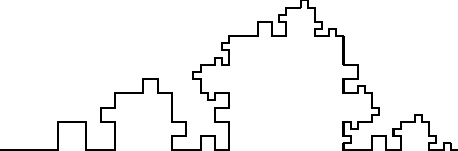
\includegraphics[width=0.27\textwidth]{fractal3}
   	\\
   	Step 1&Step 2&Step 3
    \end{tabular}
    \end{center}
    After each step, we are left with a curve. After step 1 the curve has length $\ell_1=\frac 32$. After step 2 the length is $\ell_2=\frac 94$. What is the \emph{length} $\ell_n$ of the curve after $n$ steps? Prove your assertion.
    \item Below is the result of repeating the steps in part 3 infinitely many times. What is the `length' of the resulting fractal curve?
    \begin{center}
    \includegraphics[width=0.75\textwidth]{fractal}
    \end{center}
    \item Repeat parts (c) and (d) for the \emph{area} under the curve at each step. Prove that the area between the fractal curve and the $x$-axis is $\frac 18$.
	\end{enumerate}
\end{enumerate}

\fi
%\graphicspath{{notes/7relations/}}

\section{Relations and Partitions}\label{sec:relations}

The mathematics of sets is rather basic, at least until one has a notion of how to relate elements of sets to each other. We are already familiar with examples of this:
\begin{enumerate}
  \item The usual \emph{order} of numbers (e.g. $3<7$) is a way of relating/comparing two elements of $\R$.% Recall that, as sets, order doesn't matter: $\{3,7\}=\{7,3\}$. As \emph{ordered pairs} however, $(3,7)\neq(7,3)$.
  \item A \emph{function} $f:A\to B$ relates elements in a set $A$ with those in $B$.
\end{enumerate}
It turns out that the concept of ordered pair (Cartesian product) is essential to relating elements.

\subsection{Relations}

\begin{defn}
Let $A$ and $B$ be sets. A \emph{(binary) relation} $\cR$ from $A$ to $B$ is a set of ordered pairs
\[\cR\subseteq A\times B.\]
A \emph{relation on} $A$ is a relation from $A$ to itself.\\
If $(x,y)\in\cR$ we can also write $x\,\cR\,y$, and say `$x$ is related to $y$.' Similarly $x\not\!\!\cR\,y$ means $(x,y)\not\in\cR$.
\end{defn}

\begin{examples}
\item $\cR=\{(1,3),(2,2),(2,3),(3,2),(4,1),(5,2)\}$ is a relation from $\N$ to $\N$. It is also a relation from $\{1,2,3,4,5\}$ to $\{1,2,3\}$. Various true statements about this relation include
\[(2,2)\in\cR,\qquad (4,2)\not\in\cR,\qquad 2\not\!\!\cR\,5,\qquad 3\,\cR\,2\]
\item $\cR=\Bigl([1,3)\times (3,4]\Bigr)\cup\big\{(2t+1,t^2):t\in [\frac 12,2]\big\}$ is a relation from $\R$ to $\R$. Be careful: it is easy to confuse interval notation with the notation for ordered pair!
\item The set $\cR=\{(a,a):a\in A\}$ is a relation on $A$, indeed
\[(x,y)\in \cR\iff x=y\]
defines a relation on \emph{any} set $A$. This example is where the term \emph{equivalence relation} (Section \ref{sec:equiv}) comes from. $x\,\cR\,y\iff x=y$ simply says that $\cR$ is `equals.'
\item If $A=\{\text{all humans}\}$, we may define $\cR\subseteq A\times A$ by
\[(a_1,a_2)\in \cR\iff a_1,a_2\text{ have a parent-child, or a sibling relationship.}\]
In this example, the mathematical use of the word relation is identical to that in English. For example, I am related to my sister, and my mother is related to me.
\item If $A$ is a set, then $\subseteq$ is a relation on the power set $\cP(A)$.\\
For example, if $A=\{1,2,3\}$ then $\{1\}\in\cP(A)$ and $\{1,3\}\in\cP(A)$. We'd say that $\{1\}$ is related to $\{1,3\}$ since $\{1\}\subseteq\{1,3\}$.\\
It should be clear that, under the relation $\subseteq$, that $\{1,3\}$ is not related to $\{1\}$.
\end{examples}

When $\cR$ is a relation between sets of numbers, we can often \emph{graph} the relation. Examples 1 and 2 above would be graphed as follows:
\begin{center}
\begin{minipage}{0.3\textwidth}\centering
\includegraphics[width=\textwidth]{relations-01-reln1}\\
Example 1.
\end{minipage}\qquad\qquad\qquad
\begin{minipage}{0.3\textwidth}\centering
\includegraphics[width=\textwidth]{relations-02-reln2}\\
Example 2.
\end{minipage}
\end{center}
Not all relations between sets of numbers can be graphed: for example, graphing the relation $\cR=\Q\times\Q$ is impossible!\\


\noindent\begin{minipage}{0.6\textwidth}
To refer to the introduction, the standard ordering $<$ on $\N$ is a relation, and we can graph it: for all $x,y\in\N$, we define
\[x\,\cR\,y\iff x<y\]
or equivalently,
\[\cR=\{(x,y)\in\N\times\N:x<y\}\]
\vspace*{10pt}
\end{minipage}\hfill\begin{minipage}{0.3\textwidth}
\includegraphics[width=\textwidth]{relations-25-less}
\end{minipage}\\
We can also think about functions in this language: if $f:\R\to\R$ is a function, then we could define
\[x\,\cR\,y\iff y=f(x)\]
or equivalently
\[\cR=\{(x,y)\in\R^2:y=f(x)\}\]
We will return to this viewpoint on function in the Section \ref{sec:func2}.

\subsubsection*{Basic results regarding relations}

With abstract relations, there are only a small number of things we can do.

\begin{defn}\label{defn:relnsym}
If $\cR\subseteq A\times B$ is a relation, then its \emph{inverse} $\cR^{-1}\subseteq B\times A$ is the set
\[\cR^{-1}=\{(y,x)\in B\times A:(x,y)\in\cR\}.\]
To find the elements of $\cR^{-1}$, you simply switch the components of each ordered pair in $\cR$.\\
Suppose $A=B$. We say that $\cR$ is \emph{symmetric} if $\cR=\cR^{-1}$.
\end{defn}\pagebreak[1]

\noindent The following results should seem natural, even if some of the proofs may not be obvious.

\begin{thm}\label{thm:relbasic}
Given any relations $\cR,\cS\subseteq A\times B$:
\begin{enumerate}
\item $(\cR^{-1})^{-1}=\cR$
\item $\cR\subseteq \cS\iff \cR^{-1}\subseteq \cS^{-1}$
\item $(\cR\cup \cS)^{-1}=\cR^{-1}\cup \cS^{-1}$
\item $(\cR\cap \cS)^{-1}=\cR^{-1}\cap \cS^{-1}$
\item If $A=B$, then $\cR\cup \cR^{-1}$ is symmetric
\item If $A=B$, then $\cR\cap \cR^{-1}$ is symmetric
\end{enumerate}
\end{thm}

\begin{proof}
Here are two of the arguments. Try the others yourself.
\begin{enumerate}
\item[2.] Assume that $\cR\subseteq\cS$, and suppose that $(x,y)\in\cR^{-1}$. We must prove that $(x,y)\in\cS^{-1}$. By the definition of inverse,
\begin{align*}
(x,y)\in\cR^{-1}&\implies (y,x)\in\cR\implies (y,x)\in\cS\\
&\implies (x,y)\in\cS^{-1}.
\end{align*}
Therefore $\cR^{-1}\subseteq\cS^{-1}$. For the converse, suppose that $\cR^{-1}\subseteq\cS^{-1}$. Then, by an argument similar to the above, we see that $(\cR^{-1})^{-1}\subseteq (\cS^{-1})^{-1}$. Now use 1.\ to see that
\[\cR^{-1}\subseteq\cS^{-1}\implies\cR\subseteq \cS.\]
\item[5.] By 3,
\[(\cR\cup \cR^{-1})^{-1}=\cR^{-1}\cup (\cR^{-1})^{-1}=\cR^{-1}\cup \cR=\cR\cup \cR^{-1},\]
and so $\cR\cup \cR^{-1}$ is symmetric.\qedhere
\end{enumerate}
\end{proof}

\noindent{\bf Keep your proof skills sharp!}\quad Several parts of Theorem \ref{thm:relbasic} look suspiciously similar to earlier results and it is easy to get confused. For example, 3 and 4 look almost like De Morgan's laws, except that $\cup$ and $\cap$ do not switch over. This is why it is important to be able to conjure up examples and \emph{prove} such statements. There are many facts in mathematics: trying to memorize everything is too difficult! Instead, you will be forever conjecturing and having to justify your guesses. For example, suppose that you forget results 3 and 4: it seems reasonable to conjecture that
\[(\cR\cup \cS)^{-1}=\begin{cases}
\cR^{-1}\cup \cS^{-1}\\
\qquad\text{or}\\
\cR^{-1}\cap \cS^{-1}
\end{cases}\]
Now that you have two sensible guesses, you should be able to decide the correct one by thinking about examples and, if necessary, proving your assertion!

\begin{example}
Consider Example 1 from before: $\cR=\{(1,3),(2,2),(2,3),(3,2),(4,1),(5,2)\}\subseteq\N\times\N$. This is not symmetric since, for example, $1\,\cR\,3$ but $3\not\!\!\cR\,1$. We compute
\[\cR^{-1}=\{(3,1),(2,2),(3,2),(2,3),(1,4),(2,5)\},\]
and observe that
\begin{gather*}
\cR\cap \cR^{-1}=\{(2,2), (2,3), (3,2)\}\quad\text{and}\quad \\
\cR\cup \cR^{-1}=\{(1,3),(3,1),(2,2),(2,3),(3,2),(4,1),(1,4),(5,2),(2,5)\}
\end{gather*}
are both symmetric.
\end{example}

\begin{center}
\begin{minipage}{0.35\textwidth}\centering
\includegraphics[width=\textwidth]{relations-03-relnint}\\
The relation $\cR\cap \cR^{-1}$
\end{minipage}\qquad\qquad\qquad
\begin{minipage}{0.35\textwidth}\centering
\includegraphics[width=\textwidth]{relations-04-relnun}\\
The relation $\cR\cup \cR^{-1}$
\end{minipage}
\end{center}

\noindent These pictures should confirm something intuitive: if you are able to graph a symmetric relation, then the graph will have symmetry about the line $y=x$. Indeed, $\cR^{-1}$ is obtained by reflecting $\cR$ in the line $y=x$. Recall how to graph an inverse functions from calculus\ldots

\paragraph{Self-test Questions}

	\begin{enumerate}
    \item A \emph{relation} $\cR$ from a set $A$ to a set $B$ is \underline{\phantom{a subset of $A\times B$}\qquad\qquad} 
    \item If $A\subseteq\R$, then the graph of a symmetric relation $\cR\subseteq A\times A$ has what sort of symmetry?
    \item True or false: if $\cR$ is symmetric, then it must contain an even number of elements.
  \end{enumerate}

\subsection*{Exercises}

\begin{enumerate}\renewcommand{\labelenumi}{\thesubsection.\theenumi}
  \item Let $\cR$ be the relation on $\{0,1,2\}$ defined by
  \[0\,\cR\,0\qquad 0\,\cR\,1\qquad 2\,\cR\,1\]
  \begin{enumerate}
    \item Write $\cR$ as a set of ordered pairs.
    \item What is the inverse of $\cR$?
	\end{enumerate}
	
	\item Let $\cR$ be the relation on $\R$ defined by $x\,\cR\,y\iff\nm{x-y}=1$. Draw $\cR$. Is it symmetric?
  
	\item Draw pictures of the following relations on the set of real numbers $\R$.
		\begin{enumerate}
			\item $\cR=\{(x,y):y\le x\text{ and }y\le 2\text{ and }y\le 2-x\}$.
			\item $\cS=\{(x,y):(x-4)^2+(y-1)^2\le 9\}$.
		\end{enumerate}
	Also draw the inverse of each relation.
	
	\item A relation is defined on $\N$ by $a\,\cR\,b\!\iff\! \frac ab\in\N$. Let $c,d\in\N$. Under what conditions is it permissable to write $c\,\cR^{-1}\,d$?
	
	\item Let $\cR\subseteq\{1,2,3,4\}\times\{1,2,3,4\}$ be the relation
	\[\cR=\{(1,3),(1,4),(2,2),(2,4),(3,1),(3,2),(4,4)\}.\]
	\begin{enumerate}
	  \item Compute $\cR^{-1}$.
	  \item Compute the relations $\cR\cup \cR^{-1}$ and $\cR\cap \cR^{-1}$, and check that they are symmetric.
	\end{enumerate}
  
  \item For the relation $\cR=\{(x,y):x\le y\}$ defined on $\N$, what is $\cR^{-1}$, and what is the intersection $\cR\cap\cR^{-1}$?

  \item Let $A$ be a set with $\nm A=4$. What is the maximum number of elements that a relation $\cR$ on $A$ can contain such that $\cR\cap \cR^{-1}=\emptyset$?
  
  \item Give formal proofs of the remaining cases (1, 3, 4 \& 6) of Theorem \ref{thm:relbasic}.
  
  \item Let $\cR$ be a relation on a set $A$ and define $\cS=\cR\cup\cR^{-1}$. We know that $\cS$ is symmetric. Prove that $\cS$ is the intersection of all \emph{symmetric} relations on $A$ which contain $\cR$. Otherwise said: if
  \[\mathrm T=\Bigl\{\mathcal T\subseteq A\times A:\mathcal T\text{ symmetric and }\cR\subseteq\mathcal T\bigr\}\]
  then
  \[\cS=\bigcap\limits_{\mathcal T\in \mathrm T} \mathcal T\]
  \emph{$\cS$ is known as the \emph{symmetric closure} of $\cR$.}
\end{enumerate}
\newpage


\subsection{Functions revisited}\label{sec:func2}

Now that we have the language of relations, we can properly define functions. Recall that a function $f:A\to B$ is a rule that assigns one, and only one, element of $B$ to each element of $A$. We may therefore view $f$ as a collection of ordered pairs in $A\times B$:
\[\big\{(a,f(a)):a\in A\big\}.\]
This set is nothing more than the \emph{graph} of the function, and, being a set of ordered pairs, it is a relation.

\begin{defn}\label{defn:func}
Let $\cR\subseteq A\times B$ be a relation from $A$ to $B$. The \emph{domain} and \emph{range} of $\cR$ are the sets
\begin{gather*}
\dom(\cR)=\{a\in A:(a,b)\in \cR\text{ for some }b\in B\},\\
\range(\cR)=\{b\in B:(a,b)\in \cR\text{ for some }a\in A\}.
\end{gather*}
A \emph{function} from $A$ to $B$ is a relation $f\subseteq A\times B$ satisfying the following conditions:
\begin{enumerate}
  \item $\dom(f)=A$,
  \item $(a,b_1),(a,b_2)\in f\implies b_1=b_2$.
\end{enumerate}
\end{defn}

\noindent The two conditions can be thought of as saying:
\begin{enumerate}
  \item Every element of $A$ is related to \emph{at least one} element of $B$.
  \item Every element of $A$ is related to \emph{at most one} element of $B$.
\end{enumerate}
Putting these together, we see that a relation $f\subseteq A\times B$ is a function if \emph{every} $a\in A$ is the first entry of one (and only one) ordered pair $(a,b)\in f$. The second condition is the vertical line test, familiar from calculus.

\begin{center}
\begin{minipage}{0.32\textwidth}\centering
\includegraphics[width=\textwidth]{relations-05-funcvert}\\
$b_1=b_2=f(a)$: a function
\end{minipage}\qquad\qquad\qquad\qquad
\begin{minipage}{0.32\textwidth}\centering
\includegraphics[width=\textwidth]{relations-06-funcvert}\\
$b_1\neq b_2$: not a function
\end{minipage}
\end{center}

\noindent We can also think about injectivity and surjectivity (recall Definition \ref{defn:11}) in this context. A function $f\subseteq A\times B$ is:
\begin{itemize}
  \item \emph{Injective} if no two pairs in $f$ share the same second entry.
  \item \emph{Surjective} if every $b\in B$ appears as the second entry of at least one pair in $f$.
  \item \emph{Bijective} if every $b\in B$ appears as the second entry of one (and only one) ordered pair $(a,b)\in f$.
\end{itemize}


\begin{example}
Let $A=B=\{1,2,3\}$ and consider the relation\\
\noindent\begin{minipage}{0.62\textwidth}
\[f=\{(1,3),(2,1),(3,3)\}.\]
Observe that $\dom(f)=\{1,2,3\}=A$, and that each element of $A$ appears exactly once as the first element in a pair $(a,b)\in f$. The relation therefore satisfies both conditions necessary to be a function. In more elementary language we would write $f(1)=3$, \ $f(2)=1$ and $f(3)=3$.\\[5pt]
Since 3 appears twice as a second entry of an ordered pair in $f$ we see that $f$ is \emph{not injective.}\\[5pt]
Since 2 never appears as the second entry of an ordered pair in $f$ we see that $f$ is \emph{not surjective.}
\end{minipage}\hfill\begin{minipage}{0.33\textwidth}
\centering
\includegraphics[width=\textwidth]{relations-18-reln1}\\
A function $f:A\to B$
\end{minipage}
\end{example}

\subsubsection*{The Inverse of a Function}

Since every function is a relation, it is a straightforward business to define the inverse of a function.

\begin{defn}
The \emph{inverse} of a function $f\subseteq A\times B$ is the inverse relation $f^{-1}\subseteq B\times A$.
\end{defn}

\noindent To compute an inverse relation we simply reverse the components of each ordered pair: the following should therefore be clear.

\begin{thm}\label{thm:inversedomrange}
$\dom(f^{-1})=\range(f)$ \ and \ $\range(f^{-1})=\dom(f)$.
\end{thm}

\noindent In general, you should expect the inverse of a function to be merely a relation and not a function in its own right. We shall shortly (Theorem \ref{thm:finverse}) discuss when the inverse relation is a function.

\begin{example}[cont.]
Consider the above example.\\[5pt]
\noindent\begin{minipage}{0.62\textwidth}
The inverse relation
\[f^{-1}=\{(3,1),(1,2),(3,3)\}\subseteq B\times A\]
is \emph{not} a function due to failing \emph{both} conditions of Definition \ref{defn:func}.
\begin{itemize}
  \item $\dom(f^{-1})=\{1,3\}$ is not the whole of $B$.
  \item $(3,1)\in f^{-1}$ and $(3,3)\in f^{-1}$, but $1\neq 3$.
\end{itemize}
Both failures are clearly visible in the picture.
\end{minipage}\hfill\begin{minipage}{0.33\textwidth}
\centering
\includegraphics[width=\textwidth]{relations-19-reln1}\\
$f^{-1}\subseteq B\times A$: not a function
\end{minipage}
\end{example}

\noindent Before we consider exactly when the inverse of a function is a function in its own right, we consider a few more examples.


\begin{examples}
\item\label{ex:reln1} Let $A=B=\R$ and $f=\{(x,x^2):x\in\R\}$. This is simply the function with formula $f(x)=x^2$. The inverse relation $f^{-1}\subseteq\R\times\R$ is then
\[f^{-1}=\bigl\{(x^2,x):x\in\R\bigr\}=\bigl\{(y,\pm\sqrt y):y\ge 0\bigr\}.\]
In this case, $f^{-1}$ is \emph{not a function.} In the language of Definition \ref{defn:func}:
\begin{itemize}
  \item $\dom(f^{-1})=\R^+_0\neq B$. E.g., $-1\in B$ but $-1\not\in\dom(f^{-1})$.
  \item $(4,2)$ and $(4,-2)$ are distinct elements of $f^{-1}$ with the same first entry.
\end{itemize}
\begin{center}
\begin{minipage}{0.35\textwidth}\centering
\includegraphics[width=\textwidth]{relations-20-reln2}\\
$f:A\to B$
\end{minipage}\qquad\qquad\qquad
\begin{minipage}{0.35\textwidth}\centering
\includegraphics[width=\textwidth]{relations-21-reln2}\\
$f^{-1}\subseteq B\times A$: not a function
\end{minipage}
\end{center}
It should be obvious that $f$ is neither injective nor surjective: in the language of relations,
\begin{description}
	\item[Not injective]\quad $(2,4)$ and $(-2,4)$ are distinct elements of $f$ with the same second entry.
	\item[Not surjective]\quad For instance, $-1$ never appears as the second entry of any pair in $f$.
\end{description}
Observe how these are merely a rewriting of what it means for $f^{-1}$ to fail to be a function.

\item\label{ex:reln2} Let $A=B=\R$ and $f=\{(x,x^3):x\in\R\}$, so that $f$ has formula $f(x)=x^3$. This time, the inverse is also a function and we could write $f^{-1}(y)=\sqrt[3]{y}$:
\[f^{-1}=\bigl\{(x^3,x):x\in\R\bigr\}=\bigl\{(y,\sqrt[3]{y}):y\in\R\bigr\}.\]
\begin{center}
\begin{minipage}{0.35\textwidth}\centering
\includegraphics[width=\textwidth]{relations-22-reln3}\\
$f:A\to B$
\end{minipage}\qquad\qquad\qquad
\begin{minipage}{0.35\textwidth}\centering
\includegraphics[width=\textwidth]{relations-23-reln3}\\
$f^{-1}:B\to A$ is a function
\end{minipage}
\end{center}
\end{examples}\pagebreak[2]

\noindent All three of our examples help to illustrate the following important result.

\begin{thm}\label{thm:finverse}
A relation $f^{-1}\subseteq B\times A$ is a function $\iff f$ is bijective (both injective and surjective).
\end{thm}

\begin{proof}
Recalling Definition \ref{defn:func}, we see that
\[f^{-1}\text{ is a function }\iff\begin{cases}
\dom(f^{-1})=B,\\
\qquad\text{\emph{and}}\\
(b,a_1),(b,a_2)\in f^{-1}\implies a_1=a_2.
\end{cases}\]
The first of these is equivalent to $\range(f)=B$, which says that $f$ is surjective.\\
The second is equivalent to $(a_1,b),(a_2,b)\in f\implies a_1=a_2$, which says that $f$ is injective.
\end{proof}

\noindent Here is a final example, where the function $f$ is harder to visualize.

\begin{example}
Let $A=\R$, $B=\Q$ and define $f$ using the formula 
\[f(x)=\begin{cases}
x&\text{if }x\in\Q,\\
0&\text{if }x\not\in\Q.
\end{cases}\]
In the language of relations, this is $f=\bigl\{(x,x):x\in\Q\bigr\}\cup\bigl\{(x,0):x\not\in\Q\bigr\}$.\\[2pt]
This is a surjective function since every element of $B=\Q$ appears as the second entry in an ordered pair $(a,b)\in f$. It is not injective since zero appears more than once in the second entry. For example,
\[(\sqrt 2,0),\ (\sqrt 3,0)\in f.\]
Written in the more common manner, we are observing that $f(\sqrt 3)=f(\sqrt 2)$.\\[2pt]
The inverse $f^{-1}$ is not a function, and it fails to be so precisely because $f$ is non-injective. For example
\[(0,\sqrt 2)\text{ and } (0,\sqrt 3)\text{ are distinct elements of $f^{-1}$ with the same  first component.}\]
\end{example}

\paragraph{Inverse Images}

Analogously to the concept of images of sets (Section \ref{sec:func1}), we can define the \emph{inverse image} of a subset $V\subseteq B$ under a function $f:A\to B$ by
\[f^{-1}(V)=\{a\in A:f(a)\in V\}.\]
In particular, if $\{b\}\subseteq B$ has only one element, then its inverse image is
\[f^{-1}(\{b\})=\{a\in A:f(a)=b\}.\]
Both are \emph{subsets} of $A$. For instance, in the last example the inverse image of $\{0\}$ consists of zero and all irrational numbers!
\[f^{-1}(\{0\})=\{0\}\cup(\R\setminus\Q)\]
When $f^{-1}\subseteq B\times A$ is a function, each inverse image of a singleton consists of one point of $A$: thus $f^{-1}(\{b\})=\{a\}$. \emph{Only} in such a case are we entitled to write $f^{-1}(b)=a$.\pagebreak[2]




\begin{aside}
\noindent{\bf Equality of functions}

There are two competing notions of what it means for two functions to be \emph{equal.}

\begin{description}
\item[Same domain, same graph, same codomain]\quad $f=g$ means that $f$ and $g$ are the same subset of the \emph{same} $A\times B$. This notion is preferred by set theorists because it sticks rigidly to the idea that a function is a \emph{relation,} and it requires both the domain $A$ and codomain $B$ to be explicit.
\item[Same domain, same graph]\quad $f=g$ means that $f\subseteq A\times B$, \ $g\subseteq A\times C$, and
\[(a,b)\in f\iff (a,b)\in g.\]
This notion considers what a function \emph{does} to be fundamental; if two functions do the same thing to elements of the same domain then they are the same. This looser notion of equality is used more often, especially in elementary calculus.
\end{description}

\noindent The second conception of equality, while intuitive, has a problem. For example, let
\[f:\R\to\R,\quad\text{and}\quad g:\R\to[-1,1]\quad\text{satisfy}\quad f(x)=g(x)=\sin x.\]
Although $f$ and $g$ have the same graph, the different codomains of $f$ and $g$ mean that these are \emph{different functions} with respect to the first notion. Under the second notion, they are the \emph{same function.} However, $g$ is surjective while $f$ is not, so wouldn't we prefer $f$ and $g$ to be non-equal?\footnote{In elementary calculus, we usually say that a function is invertible if it is 1--1. In order for this to make sense, we have to ignore surjectivity and use the second notion of functional equality.}\\


\noindent The same problem does not arise when considering domains. For example, in calculus you might have compared functions such as
\[f(x)=x^2+2,\quad\text{and}\quad g(x)=\frac{(x^2+2)(x-1)}{x-1}.\]
The implied domains of these functions are $\dom(f)=\R$ and $\dom(g)=\R\setminus\{1\}$. Even though these have the same graph whenever \emph{both} are defined, regardless of which notion you choose we have $f\neq g$, since the functions have \emph{different domains.}
\end{aside}

\paragraph{Self-test Questions}

	\begin{enumerate}
    \item What does it mean for a \emph{relation} $\cR\subseteq A\times B$ to be a \emph{function}?
    \item If $f\subseteq A\times B$ is a function, what does it mean, in the language of relations, for $f$ to be \emph{injective}? \emph{Surjective}?
    \item True or false: a relation $\cR$ has a domain and range if and only if it is a function.
  \end{enumerate}


\subsection*{Exercises}

\begin{enumerate}\renewcommand{\labelenumi}{\thesubsection.\theenumi}
  \item Suppose that $f\subseteq\{1,2,3,4\}\times\{1,2,3,4,5,6,7\}$ is the relation
  \[f=\{(1,1),(2,3),(3,5),(4,7)\}.\]
  \begin{enumerate}
    \item Show that $f$ is a function $f:\{1,2,3,4\}\to\{1,2,3,4,5,6,7\}$. Can you find a concise formula $f(x)$ to describe $f$?
    \item Is $f$ injective? Justify your answer.
    \item Suppose that $g\subseteq\{1,2,3,4\}\times B$ is another relation so that the \emph{graphs} of $f$ and $g$ are identical: i.e.
    \[\bigl\{(a,f(a)):a\in\{1,2,3,4\}\bigr\}=\bigl\{(a,g(a)):a\in\{1,2,3,4\}\bigr\}.\] \emph{as sets.} If $g$ is a bijective function, what is $B$?
  \end{enumerate}
  
  \item Decide whether each of the following relations are functions. For those which are, decide whether the function is injective and/or surjective.
  \begin{enumerate}
    \item $\cR=\{(x,y)\in[-1,1]\times[-1,1]:x^2+y^2=1\}$
    \item $\cS=\{(x,y)\in[-1,1]\times[0,1]:x^2+y^2=1\}$
    \item $\mathcal T=\{(x,y)\in[0,1]\times[-1,1]:x^2+y^2=1\}$
    \item $\mathcal U=\{(x,y)\in[0,1]\times[0,1]:x^2+y^2=1\}$
  \end{enumerate}
  
  \item In Example \ref{ex:reln2} on page \pageref{ex:reln2}, explain why the function $f$ is both injective and surjective using the language of relations: i.e., in the same manner as we analyzed Example \ref{ex:reln1}.
  
  \item For each of the examples on page \pageref{ex:reln2}, compute the following inverse images:
  \begin{enumerate}
    \item $f^{-1}(\{0,1\})$
    \item $f^{-1}\Big([0,1)\Big)$
    \item $f^{-1}\Big((-\infty,0]\Big)$
    \item $f^{-1}\Big(\{-8\}\cup[-7,2]\cup (3,9)\Big)$
  \end{enumerate}
  
  \item\begin{enumerate}
    \item Express the function $f:\R\to\R:x\mapsto x^4+3$ as a relation.
    \item What is the inverse relation $f^{-1}$?
    \item Use Definition \ref{defn:func} to prove that the relation $f^{-1}$ is \emph{not} a function.
    \item Prove directly from Definition \ref{defn:11} that $f$ is not injective and not surjective. Compare your arguments with your answer to part (c).
  \end{enumerate}
  
  \item Repeat the previous question for $f:\R\to\R:x\mapsto \sqrt{x^2-4x+5}$.
  
  \item Give a formal proof of Theorem \ref{thm:inversedomrange}.
  
  \item Prove or disprove the following: if $f:A\to B$ is a function, and $U,V\subseteq B$, then
  \[f^{-1}(U\cap V)=f^{-1}(U)\cap f^{-1}(V)\]
\end{enumerate}
\newpage

\subsection{Equivalence Relations}\label{sec:equiv}

In mathematics, the notion of \emph{equality} is not as simple as one might think. The idea of two numbers being equal is straightforward, but suppose we want to consider two paths between given points as `equal' if and only if they have the same length? Since two `equal' paths might look very different, is this a good notion of equality? Mathematicians often want to gather together objects that have a common property and then treat them as if they were a single object. This is done using equivalence relations and equivalence classes.\\

\noindent First recall the alternative notation for a relation on a set $A$: if $\cR\subseteq A\times A$ is a relation on $A$, then $x\,\cR\,y$ has the same meaning as $(x,y)\in\cR$. We might read $x\,\cR\,y$ as `$x$ is $\cR$-related to $y$.'

\newsavebox\mybox
\sbox{\mybox}{\emph{Transitivity}}
\def\refl{\makebox[\wd\mybox][l]{\emph{Reflexivity}}}
\def\symm{\makebox[\wd\mybox][l]{\emph{Symmetry}}}
\def\trans{\makebox[\wd\mybox][l]{\emph{Transitivity}}}

\begin{defn}
A relation $\cR$ on a set $A$ may be described as \emph{reflexive, symmetric} or \emph{transitive} if it satisfies the following properties:
	\begin{ptabular}{\trans}
		\refl&$\forall x\in A$, \ $x\,\cR\,x$\hfill(every element of $A$ is related to itself)\\
		\symm&$\forall x,y\in A,\ x\,\cR\,y\implies y\,R\,x$\hfill(if $x$ is related to $y$, then $y$ is related to $x$)\\
		\trans&$\forall x,y,z\in A,\ x\,\cR\,y$ \ and \ $y\,\cR\,z\implies x\,\cR\,z$\hfill(if $x$ is related to $y$, and $y$ is related to $z$,\newline
		\phantom{bob}\hfill then $x$ is related to $z$)
	\end{ptabular}
\end{defn}

Symmetry is exactly the same notion as in Definition \ref{defn:relnsym}.

\begin{examples}
\item Let $A=\R$ and let $\cR$ be $\le$. Thus $2\le 3$, but $7\nleq 4$. We check whether $\cR$ satisfies the above properties.
	\begin{eptabular}{\trans}
		\refl&True. $\forall x\in\R$, \ $x\le x$.\\
		\symm&False. For example, $2\le 3$ but $3\nleq 2$.\\
		\trans&True. $\forall x,y,z\in\R$, if $x\le y$ and $y\le z$, then $x\le z$.
	\end{eptabular}
\item Let $A$ be the set of lines in the plane and define $\ell_1\,R\,\ell_2\iff \ell_1$ and $\ell_2$ intersect.\\
\noindent\begin{minipage}{0.65\textwidth}
	\noindent\begin{eptabular}{\trans}
		\refl&True. Every line intersects itself, so $\ell\,\cR\,\ell$ for all $\ell\in A$.\\
		\symm&True. For all lines $\ell_1,\ell_2\in A$, if $\ell_1$ intersects $\ell_2$, then $\ell_2$ intersects $\ell_1$..\\
		\trans&False. As the picture illustrates, we may let $\ell_1$ and $\ell_3$ be parallel lines, and $\ell_2$ cross both of these. Then $\ell_1\,\cR\,\ell_2$ and $\ell_2\,\cR\,\ell_3$, but $\ell_1\not\!\!\cR\,\ell_3$.
	\end{eptabular}
\end{minipage}\hfill
		\begin{minipage}{0.3\textwidth}
	\includegraphics[width=\textwidth]{relations-07-parallel}
		\end{minipage}
\end{examples}

\begin{defn}
An \emph{equivalence relation} is a relation $\sim$ which is reflexive, symmetric and transitive.
\end{defn}

\noindent The symbol $\sim$ is almost universally used for an abstract equivalence relation. It can be read as `related to,' `tilde,' or `twiddles.' The two examples above are \emph{not} equivalence relations because they fail one of the three conditions. We now exhibit the simplest equivalence relation.

\begin{example}
Equals `=' is an equivalence relation on any set, hence the name!
\end{example}

\noindent Read the definitions of reflexive, symmetric and transitive until you are certain of this fact. There are countless other equivalence relations: here are a few.

\begin{examples}
	\item For all $x,y\in\Z$, we define the relation $\sim$ by
	\[x\sim y\iff x-y\ \text{ is even.}\]
	We claim that $\sim$ is an equivalence relation on $\Z$.
	\begin{eptabular}{\trans}
		\refl&$\forall x\in\Z,\ x-x=0$ is even, hence $x\sim x$.\\
		\symm&$\forall x,y\in\Z,\ x\sim y\implies x-y$ is even $\implies y-x$ is even $\implies y\sim x$.\\
		\trans&$\forall x,y,z\in\Z$, if $x\sim y$ and $y\sim z$, then $x-y$ and $y-z$ are even. But the sum of two even numbers is even, hence $x-z=(x-y)+(y-z)$ is even, and so $x\sim z$.
	\end{eptabular}
	
	\item Let $A=\{$all students taking this course$\}$. For all $x,y\in A$, let
	\[x\sim y\iff x\ \text{ achieves the same letter-grade as $y$.}\]
	Then $\sim$ is an equivalence relation on $A$; here is the proof.
	\begin{eptabular}{\trans}
		\refl&$\forall x\in A,\ x\sim x$ since everyone scores the same as themself!\\
		\symm&$\begin{array}[t]{@{}rl}
		\forall x,y\in A,\ x\sim y&\implies x\ \text{achieves the same letter-grade as $y$}\\
		&\implies y\ \text{achieves the same letter-grade as $x$}\\
		&\implies y\sim x
		\end{array}$\\
		\trans&$\forall x,y,z\in A$, if $x\sim y$ and $y\sim z$, then $x$ achieves the same as $y$ who achieves the same as $z$, whence $x$ achieves the same as $z$. Thus $x\sim z$.
	\end{eptabular}

	\item We define an equivalence relation on $\Z$ by
	\[\forall x,y\in\Z,\ \ x\sim y\iff x^2\equiv y^2\pmod 5.\]
		\begin{eptabular}{\trans}
		\refl&$\forall x\in\Z,\ x\sim x$ since $x^2$ is always congruent to itself!\\
		\symm&$\begin{array}[t]{@{}rl}
		\forall x,y\in\Z,\ x\sim y&\implies x^2\equiv y^2\pmod 5\\
		&\implies y^2\equiv x^2\pmod 5\\
		&\implies y\sim x
		\end{array}$\\
		\trans&$\forall x,y,z\in\Z$, if $x\sim y$ and $y\sim z$, then $x^2\equiv y^2$ and $y^2\equiv z^2\pmod 5$. But then $x^2\equiv z^2\pmod 5$ and so $x\sim z$.
	\end{eptabular}
\end{examples}

\noindent The most important thing to observe in each of these examples is that {\bf an equivalence relation separates elements of a set into subsets where elements share a common property} (even/oddness, letter-grade, etc.). The next definition formalizes this idea.

\begin{defn}\label{defn:equivrel}
Let $\sim$ be an equivalence relation on a set $X$. The \emph{equivalence class} of an element $x\in X$ is the set
\[[x]=\{y\in X:y\sim x\}.\]
Otherwise said, $y\sim x\iff y\in[x]$. The set of all equivalence classes is known as the \emph{quotient} of $X$ by $\sim$ or simply `$X$ mod $\sim$,' and is denoted
\[\quotient X\sim=\Big\{[x]:x\in X\Big\}\]
\end{defn}

\noindent Let us think about the definition of equivalence class in the context of our previous examples.

\begin{examples}
	\item $[0]=\{y\in\Z:y\sim 0\}=\{y\in\Z:y\text{ is even}\}$ is the set of even numbers. Note that $[0]=[2]=[4]=[6]$, etc. The other equivalence class is $[1]=\{y\in\Z:y-1\text{ is even}\}$, which is the set of odd numbers. The quotient set is
	\[\smash{\quotient \Z\sim}=\bigl\{[0],[1]\bigr\}=\bigl\{\{\text{even numbers}\},\{\text{odd numbers}\}\bigr\}.\]

	\item There is one equivalence class for each letter grade awarded. Each equivalence class contains all the students who obtain a particular letter-grade. If we call the equivalence classes $\mathrm{A^+,A,A^-,B^+,\ldots,F}$, where, say, $\mathrm B=\{$students obtaining a B-grade$\}$, then
	\[\smash{\quotient{\{\text{Students}\}}{\sim}}=\{\mathrm{A^+,A,A^-,B^+,\ldots,F}\}.\]

	\item The equivalence classes for this example are a little tricky. First observe that
	\[x\equiv y\tpmod 5\implies x^2\equiv y^2\tpmod 5,\]
	so that there are at most five equivalence classes; those of 0, 1, 2, 3 and 4. Are they distinct?	If we square each of these and consider the remainder modulo 5, we obtain
	\[\begin{array}{l@{}r|c|c|c|c|c}
	x&\tpmod 5&0&1&2&3&4\\\hline
	x^2&\tpmod 5&0&1&4&4&1
	\end{array}\]
	Notice that $1\sim 4$, so they share an equivalence class. Similarly $2\sim 3$. Indeed the distinct equivalence classes are
	\begin{gather*}
	[0]=\{x\in\Z:x\equiv 0\tpmod 5\}\\
	[1]=\{x\in\Z:x\equiv 1,4\tpmod 5\}\\
	[2]=\{x\in\Z:x\equiv 2,3\tpmod 5\}
	\end{gather*}
	In this case the quotient is the set
	\[\smash{\quotient{\Z}{\sim}}=\Bigl\{[0],[1],[2]\Bigr\}.\]
\end{examples}%\pagebreak[2]

\noindent Here is one further example of an equivalence relation, this time on $\R^2$. Be careful with the notation: $\R^2=\R\times\R$ is already a Cartesian product, so a relation on $\R^2$ is a subset of $\R^2\times\R^2$!


\begin{example}\label{ex:equivcircle}
Let $\sim$ be the relation on $\R^2$ defined by $(x,y)\sim(v,w)\iff x^2+y^2=v^2+w^2$. We claim that this is an equivalence relation.
	\begin{ptabular}{\trans}
		\refl&$\forall (x,y)\in\R^2,\ x^2+y^2=x^2+y^2$.\\
		\symm&$\begin{array}[t]{@{}rl}
		\forall (x,y),(v,w)\in\R^2,\ (x,y)\sim(v,w)&\implies x^2+y^2=v^2+w^2\\
		&\implies v^2+w^2=x^2+y^2\\
		&\implies (v,w)\sim(x,y)
		\end{array}$\\
		\trans&$\forall (x,y),(v,w),(p,q)\in\R^2$, if $(x,y)\sim (v,w)$ and $(v,w)\sim (p,q)$, then $x^2+y^2=v^2+w^2$ and $v^2+w^2=p^2+q^2$. But then $x^2+y^2=p^2+q^2$ and so $(x,y)\sim (p,q)$.
	\end{ptabular}\\
	
	$\sim$ is therefore an equivalence relation. But what are the equivalence classes? By definition,
\[[(x,y)]=\Bigl\{(v,w)\in\R^2:v^2+w^2=x^2+y^2\Bigr\}.\]
\noindent\begin{minipage}{0.6\textwidth}
This isn't particularly helpful. Indeed it is easier to think of each of these sets as
\[\Bigl\{(v,w)\in\R^2:v^2+w^2\text{ is \emph{constant}}\Bigr\}.\]
Each equivalence class is therefore a \emph{circle} centered at the origin! Some of the equivalence classes are drawn in the picture: the class $[(1,0)]$ is highlighted. Moreover, the quotient set is
\[\quotient{\R^2}{\sim}=\{\text{circles centered at the origin}\}.\]
\end{minipage}\qquad
\begin{minipage}{0.35\textwidth}
\includegraphics[width=\textwidth]{relations-24-circles}
\end{minipage}
\end{example}

\paragraph{Self-test Questions}

	\begin{enumerate}
    \item True or false: a relation $\sim$ on a set $X$ is \emph{reflexive} if $\exists x\in X$ such that $x\sim x$.
   	\item An \emph{equivalence relation} satisfies which three properties? What do they mean?
    \item Suppose that $x,y,z\in X$ and $\sim$ is an equivalence relation on $X$. Express each of the following assertions in terms of the properties satisfied by an equivalence relation.
    \begin{enumerate}
      \item $x\in[y]$ and $y\in[z]\implies x\in[z]$.
      \item $x\in[x]$.
      \item $x\in[y]\iff y\in[x]$.
  	\end{enumerate}
  \end{enumerate}

\subsection*{Exercises}

\begin{enumerate}\renewcommand{\labelenumi}{\thesubsection.\theenumi}
	\item A relation $\cR$ is \emph{antisymmetric} if $((x,y)\in \cR)\wedge((y,x)\in \cR)\implies x=y$. Give examples of relations $\cR$ on $A=\{1,2,3\}$ having the stated property.
	\begin{enumerate}
		\item $\cR$ is both symmetric and antisymmetric.
		\item $\cR$ is neither symmetric nor antisymmetric.
		\item $\cR$ is transitive but $\cR\cup \cR^{-1}$ is not transitive.
	\end{enumerate}
	
	\item Let $\cS=\{(x,y)\in\R^2:\sin^2x+\cos^2y=1\}$.
	\begin{enumerate}
	  \item Give an example of two real numbers $x,y$ such that $x\,\cS\,y$.
	  \item Is $\cS$ reflexive? Symmetric? Transitive? Justify your answers.
	\end{enumerate}

	\item Each of the following relations $\sim$ is an equivalence relation on $\R^2$. Identify the equivalence classes and draw several of them.
	\begin{enumerate}
		\item $(a,b)\sim(c,d)\iff ab=cd$.
	  \item $(v,w)\sim(x,y)\iff v^2w=x^2y$.
	\end{enumerate}
	
  \item\begin{enumerate}
  \item Let $\sim$ be the relation defined on $\Z$ by $a\sim b\iff a+b$ is even. Show that $\sim$ is an equivalence relation and determine the distinct equivalence classes.
  \item Suppose that `even' is replaced by `odd' in part (a). Which of the properties reflexive, symmetric, transitive does $\sim$ possess?
  \end{enumerate}

  \item For each of the following relations $\cR$ on $\Z$, decide whether $\cR$ is reflexive, symmetric, or transitive, and whether $\cR$ is an equivalence relation.
	\begin{enumerate}
		\item $a\,\cR\,b \iff a\equiv b\pmod 3 \textbf{ or } a\equiv b\pmod 4$.
		\item $a\,\cR\,b \iff a\equiv b\pmod 3 \textbf{ and } a\equiv b\pmod 4$.
	\end{enumerate}

	\item For the purposes of this question, we call a real number $x$ \emph{small} if $\nm x\le 1$. Let $\cR$ be the relation on the set of real numbers defined by
	\[x\,\cR\,y \iff x-y \text{ is small}.\]
	\emph{Prove or disprove}: $\cR$ is an equivalence relation on $\R$.

	\item Let $A=\{1,2,3,4,5,6\}$. The distinct equivalence classes resulting from an equivalence relation $\sim$ on $A$ are $\{1,4,5\}$, $\{2,6\}$, and $\{3\}$. What is $\sim$? Give your answer as a subset of $A\times A$.

	\item $\subseteq$ is a relation on any set of sets. Is $\subseteq$ reflexive, symmetric, transitive? Prove your assertions.

	\item Let $S$ be the set of all polynomials of degree at most 3. An element $s\in S$ can then be expressed as
  \[s(x)=ax^3+bx^2+cx+d,\qquad\text{where $a,b,c,d\in\R$.}\]
  A relation $\cR$ on $S$ is defined by
  \[p\,\cR\,q\iff p\text{ and $q$ have a common root.}\]
  For example $p(x)=(x-1)^2$ and $q(x)=x^2-1$ have the root 1 in common so that $p\,\cR\,q$. Determine which of the properties reflexive, symmetric and transitive are possessed by $\cR$.

  \item Let $A=\{2^m:m\in\Z\}$. A relation $\sim$ is defined on the set $\Q^+$ of positive rational numbers by
  \[a\sim b\iff \frac ab\in A\]
  \begin{enumerate}
    \item Show that $\sim$ is an equivalence relation.
    \item Describe the elements in the equivalence class $[3]$.
  \end{enumerate}

  \item A relation is defined on the set $A=\{a+b\sqrt 2:a,b\in\Q,\,a+b\sqrt 2\neq 0\}$ by $x\sim y\iff \frac xy\in\Q$. Show that $\sim$ is an equivalence relation and determine the distinct equivalence classes.

	\item The \emph{reflexive, symmetric} and \emph{transitive closures} of a relation $\cR$ are defined respectively as the smallest relations containing $\cR$ which also exhibit the given property. Find each of the three closures of $\cR=\{(1,2),(2,3),(3,3)\}\subseteq\Z\times\Z$.

	\item Recall the description of the real projective line (page \pageref{ex:projline}): if $A_m$ is the line through the origin with gradient $m$, then
	\[\pr(\R^2)=\{A_m:m\in\R\cup\{\infty\}\}.\]
	Define a relation $\sim$ on $\R^2_*=\R^2\setminus\{(0,0)\}$ by $(a,b)\sim(c,d)\iff ad=bc$.
	\begin{enumerate}
	  \item Prove that $\sim$ is an equivalence relation.
	  \item Find the equivalence classes of $\sim$. How do the equivalence classes differ from the lines $A_m$?
	\end{enumerate}
  
	\item Suppose that $\cR,\cS$ are relations on some set $X$. Define the \emph{composition} $\cR\circ \cS$ to be the relation
	\[(a,c)\in \cR\circ \cS\iff \exists b\in X\text{ such that }(a,b)\in \cR\text{ and }(b,c)\in \cS.\]
	\begin{enumerate}
		\item If $\cR=\{(1,1),(1,2),(2,3),(3,1),(3,3)\}$ and $\cS=\{(1,2),(1,3),(2,1),(3,3)\}$, find $\cR\circ \cS$.
		\item Suppose that $\cR$ and $\cS$ are reflexive. Prove that $\cR\circ \cS$ is reflexive.
		\item Suppose that $\cR$ and $\cS$ are symmetric. Prove that $(x,y)\in \cR\circ \cS\iff (y,x)\in \cS\circ \cR$.
		\item Give an example of symmetric relations $\cR,\cS$ such that $\cR\circ \cS$ is \emph{not} symmetric. Conclude that if $\cR,\cS$ are equivalence relations, then $\cR\circ \cS$ need not be an equivalence relation.
	\end{enumerate}

  \item (\emph{Only for those who have studied Linear Algebra}) Let $\sim$ be the relation on the set of $2\times 2$ real matrices given by $A\sim B\iff\exists M$ such that $B=MAM^{-1}$.
  \begin{enumerate}
    \item Prove that $\sim$ is an equivalence relation.
    \item What is the equivalence class of the identity matrix?
    \item Show that $\left(\begin{smallmatrix}
    -11&15\\-5&9
    \end{smallmatrix}\right)\sim \left(\begin{smallmatrix}
    4&10\\0&-6
    \end{smallmatrix}\right)$ (\emph{Hint: think about diagonalizing})
    \item (Hard) Suppose that $L:\R^2\to\R^2$ is a linear map and $\beta,\gamma$ are bases of $\R^2$. Suppose that $A=[L]_\beta$ and $B=[L]_\gamma$ are the matrix representations of $L$ with respect to the two bases. Prove that $A\sim B$.
    \item (Hard) Suppose that $A,B$ have the same, but distinct, eigenvalues $\lambda_1\neq\lambda_2$. Prove that $A\sim B$. \emph{Again use diagonalization, the challenge here is to make your proof work even when the eigenvalues are complex numbers.}
	\end{enumerate}
\end{enumerate}
\newpage


\subsection{Partitions}

Recall the important observation about our equivalence relation examples: every element of the original set of objects ends up in \emph{exactly one equivalence class.} For instance, every integer is either even or odd but not both. The equivalence classes \emph{partition} the original set in the same way that cutting a cake partitions the crumbs: each crumb ends up in exactly one slice. We shall prove in a moment that equivalence relations \emph{always} do this. Before doing so we reverse the discussion.

\begin{defn}\label{defn:partition}
Let $X$ be a set and $\{A_n:n\in I\}$ be a collection of non-empty subsets $A_n\subseteq X$. We say that $X$ is \emph{partitioned by} the collection of subsets if
\begin{enumerate}
\item $X=\bigcup\limits_{n\in I}A_n$.\hfill(the $A_n$ together make up $X$)\\[-10pt]
\item If $A_m\neq A_n$, then $A_m\cap A_n=\emptyset$.\hfill(\emph{distinct} $A_n$ are pairwise disjoint\footnote{Recall that two sets $A,B$ are \emph{disjoint} if $A\cap B=\emptyset$: see Definition \ref{defn:unionint}. In this definition we \emph{don't} require the sets $A_n$ all to be different, some could be identical to each other.})
\end{enumerate}
We describe the collection $\cA$ as a \emph{partition} of $X$.
\end{defn}

\noindent The conditions can be viewed as saying that every element of $X$ lies in (1.) \emph{at least one} subset $A_n$ and (2.) \emph{at most one} subset $A_n$: otherwise said, every element of $X$ lies in \emph{exactly one} subset.

\begin{example}
Partition the set $X=\{1,2,3,4,5\}$ into subsets
\[A_1=\{1,3\},\qquad A_2=\{2,4\},\qquad A_3=\{5\}.\]
Now consider the relation $\cR$ on $X$, defined by
\[\cR=\{(1,1),(1,3),(3,1),(3,3),(2,2),(2,4),(4,2),(4,4),(5,5)\}.\]
What does $\cR$ have to do with the partition? It should be clear that $\cR$ could be defined by insisting that
\[x\,\cR\,y\iff \text{$x$ and $y$ are in the \emph{same} subset $A_n$.}\]
Run through your mental checklist: is $\cR$ reflexive? symmetric? transitive? Indeed $\cR$ is an equivalence relation! Moreover, the equivalence classes of $\cR$ are precisely the sets $A_1,A_2$ and $A_3$. For instance, 1 is related to itself and 3, but isn't related to anything else. Indeed
\[[1]=[3]=\{1,3\}=A_1,\qquad [2]=[4]=\{2,4\}=A_2,\qquad [5]=\{5\}=A_5.\]
\end{example} 

\noindent The example suggests that partitioning a set defines a natural equivalence relation. Combining this with our observations in the previous section and you should be starting to believe that \emph{partitions and equivalence relations are essentially the same thing.} Before we prove this important fact, here are some further examples of partitions.

\begin{examples}
\item The integers can be partitioned according to their remainder modulo 3: define
\[A_r=\{z\in\Z:z\equiv r\tpmod 3\}.\]
Then $\Z=A_0\cup A_1\cup A_2$. This is certainly a partition:
\begin{itemize}
  \item Every integer $z$ has remainder of 0, 1 or 2 after division by 3, and so every integer is in some set $A_r$.
  \item No integer has two distinct remainders modulo 3, so the sets $A_0,A_1,A_2$ are disjoint.
\end{itemize}
\item\label{ex:cong} More generally, if $n\in\N$, then the set of integers $\Z$ is partitioned into $n$ sets $A_0,\ldots,A_{n-1}$ where
\[A_r=\{z\in\Z:z\equiv r\pmod n\}\]
is the set of integers with remainder $r$ upon dividing by $n$. We are appealing to the Division Algorithm (Theorem \ref{thm:div}) which tells us that every integer $z$ has a \emph{unique remainder} $r\in\{0,1,\ldots,n-1\}$.
\item The set of real numbers $\R$ is partitioned into the sets of rational and irrational numbers: $\R=\Q\cup(\R\setminus\Q)$.
\end{examples}

\noindent Finally, here is an example of a relation which doesn't produce a partition.

\begin{example}\label{ex:partnot}
Let $X=\{1,2,3,4\}$ and define a relation $\cR$ on $X$ by
\[\cR=\{(1,3),(1,4),(2,2),(2,3),(3,1),(3,2),(4,3),(4,4)\}.\]
Also define the subsets
\[A_n=\{x\in X:(n,x)\in\cR\}.\]
Thus $A_n$ is the set of all elements of $X$ which are related to $n$. We quickly see that
\[A_1=\{3,4\},\quad A_2=\{2,3\},\quad A_3=\{1,2\},\quad A_4=\{3,4\}.\]
The collection of sets $A_n$ is as follows:
\[\{A_n\}_{n\in X}=\bigl\{A_1,A_2,A_3,A_4\bigr\}=\Bigl\{\{3,4\},\{2,3\},\{1,2\}\Bigr\},\]
where we only have \emph{three} sets in the collection since $A_4=A_1$. This collection is not a partition because, for instance, $2\in \{2,3\}\cap\{1,2\}$. In the language of Definition \ref{defn:partition}, we have
\[\{2,3\}\neq\{1,2\}\quad\text{but}\quad \{2,3\}\cap\{1,2\}\neq\emptyset.\]
More importantly, you should convince yourself that $\cR$ is \emph{not} an equivalence relation.
\end{example}

\subsubsection*{Equivalence Relations and Partitions}

Before we present the fundamental result of the chapter, we prove a helpful lemma.

\begin{lemm}\label{lemm:preequiv}
Suppose that $\sim$ is an equivalence relation. Then $x\sim y\iff [x]=[y]$.
\end{lemm}

\begin{proof}
\begin{description}
\item[$(\Leftarrow)$]\quad By reflexivity, $x\in[x]$. If $[x]=[y]$, then we have $x\in[y]$. Finally, recalling Definition \ref{defn:equivrel}, we see that that this is the same as saying $x\sim y$.
\item[$(\Rightarrow)$]\quad Suppose that $x\sim y$. We begin by showing the inclusion $[x]\subseteq [y]$. Let $z\in[x]$, then
\[z\sim x\ \text{ and }\ x\sim y\implies z\sim y\implies z\in[y].\tag*{(Transitivity)}\]
Therefore $[x]\subseteq[y]$. By symmetry, we also have $y\sim x$: repeating the argument yields $[y]\subseteq [x]$, and thus $[x]=[y]$.\qedhere
\end{description}
\end{proof}

\begin{thm}\label{thm:equivpart}
Let $X$ be any set.
\begin{enumerate}
\item If $\sim$ is an equivalence relation on $X$, then $X$ is partitioned by the equivalence classes of $\sim$.
\item If $\{A_n:n\in I\}$ is a partition of $X$, then the relation $\sim$ on $X$ defined by
\[x\sim y\iff \exists n\in I\text{ such that $x\in A_n$ and }y\in A_n\]
is an equivalence relation.
\end{enumerate}
\end{thm}

\begin{center}
\includegraphics[width=0.7\textwidth]{relations-08-part}\\
Each element of $X$ ends up in exactly one subset. In the language of the Theorem, we have\\[5pt]
$A_1=[a]$,\quad $A_2=[b]=[c]$,\quad $b\sim c$,\quad $a\nsim b$, \quad $a\nsim c$.
\end{center}

Some things to consider while reading the proof:
\begin{itemize}
  \item Think about the picture! The result is nothing more than the notion of partitioning a cake by cutting it into slices. The slices are the equivalence classes of the obvious relation: two crumbs are related if and only if they lie in the same slice. The algebra that follows merely confirms that the picture is telling a legitimate story.
  \item In part 1.\ of the proof, look for where the reflexive, symmetric and transitive assumptions about $\sim$ are used. Why do we need $\sim$ to be an equivalence relation? Why does the proof fail if any of the three assumptions are dropped?
  \item Similarly, in part 2., look for where we use both parts of the definition of partition. Why are both assumptions required?
\end{itemize}



\begin{proof}
\begin{enumerate}
\item Assume that $\sim$ is an equivalence relation on $X$. To prove that the equivalence classes of $\sim$ partition $X$, we must show two things:
\begin{enumerate}
  \item That every element of $X$ is in some equivalence class.
  \item That the distinct equivalence classes are pairwise disjoint: if $[x]\neq[y]$, then $[x]\cap[y]=\emptyset$.
\end{enumerate}
For (a), we only need reflexivity: $\forall x\in X$ we have $x\sim x$. Otherwise said, $x\in[x]$, whence every element of $X$ is in the equivalence class defined by itself.\\[5pt]
For (b), we prove by the contrapositive method and show that $[x]\cap [y]\neq\emptyset\implies [x]=[y]$.\\
Assume that $[x]\cap [y]\neq\emptyset$. Then $\exists z\in [x]\cap [y]$. This gives
\begin{align*}
z\sim x\ \text{ and }\ z\sim y&\implies x\sim z\ \text{ and }\ z\sim y\tag*{(Symmetry)}\\*
&\implies x\sim y\tag*{(Transitivity)}\\*
&\implies [x]=[y]\tag*{(Lemma \ref{lemm:preequiv})}
\end{align*}
We have proved (b) and therefore part 1.\ of the theorem.
\item Now suppose that $\{A_n:n\in I\}$ is a partition of $X$ and define $\sim$ by
\[x\sim y\iff \exists n\in I\text{ such that $x\in A_n$ and $y\in A_n$.}\]
We must prove the reflexivity, symmetry and transitivity of $\sim$.
\begin{eptabular}{\trans}
	\refl&Every $x\in X$ is in some $A_n$. Thus $x\sim x$ for all $x\in X$.\\
	\symm&If $x\sim y$, then $\exists n\in I$ such that $x,y\in A_n$. But then $y,x\in A_n$ and so $y\sim x$.\\
	\trans&Let $x\sim y$ and $y\sim z$. Then $\exists p,q\in I$ such that $x,y\in A_p$ and $y,z\in A_q$. Since $\{A_n:n\in I\}$ is a partition and $y\in A_p\cap A_q$, we necessarily have $A_p=A_q$. Thus $x,z\in A_p$ and so $x\sim z$.
\end{eptabular}

We have shown $\sim$ is an equivalence relation, and the proof is complete.\qedhere
\end{enumerate}
\end{proof}
	
\noindent Reading the proof carefully, you should see that reflexivity in part 2.\ comes from the fact that $X=\bigcup\limits_{n\in I}A_n$, while transitivity is due to the pairwise disjointness of the pieces of the partition. Symmetry is essentially free because the definition of $\sim$ is symmetric in $x$ and $y$.\\

\noindent The ability to partition sets and view the resulting subsets as individual objects is crucial to advanced mathematics. The importance of the Theorem comes from the fact that equivalence relations provide a straightforward \emph{algebraic} method of working with partitions.


\subsubsection*{Geometric Examples}

The language of equivalence relations and partitions is used heavily in geometry and topology to describe complex shapes. We finish this section with several examples. Since examples of partitions are especially easy to visualize with curves in the plane, we first return to the example on page \pageref{ex:equivcircle} and describe things in our new language.

\begin{example}
For each real number $r\ge 0$, define the set\\
\noindent\begin{minipage}{0.63\textwidth}
\[A_r=\bigl\{(x,y)\in\R^2:x^2+y^2=r^2\bigr\}.\]
This is simply the circle of radius $r$ centered at the origin. We check that $\{A_r:r\in\R^+_0\}$ is a partition of $\R^2$.
\begin{itemize}
  \item Every point of the plane lies on some circle. Precisely, $(x,y)\in A_{\sqrt{x^2+y^2}}$ since $\sqrt{x^2+y^2}$ is the distance of $(x,y)$ from the origin. Thus \smash{$\R^2=\bigcup\limits_{r\in\R^+_0}A_r$.}
  \item If $r_1\neq r_2$, then the concentric circles $A_{r_1}$ and $A_{r_2}$ do not intersect. Thus $A_{r_1}\cap A_{r_2}=\emptyset$.
\end{itemize}
\end{minipage}\hfill
\begin{minipage}{0.32\textwidth}
\includegraphics[width=\textwidth]{relations-09-circles}
\end{minipage}\\

\noindent Now define a relation $\sim$ on $\R^2$ via
\[(x,y)\sim(v,w)\iff \exists r\ge 0\text{ such that $(x,y),(v,w)$ both lie on the circle $A_r$}.\]
By Theorem \ref{thm:equivpart} this is an equivalence relation. We can also check explicitly: dropping any mention of the radius $r$, we see that
\[(x,y)\sim(v,w)\iff x^2+y^2=v^2+w^2.\]
This is exactly the equivalence relation described on page \pageref{ex:equivcircle}. The equivalence classes are precisely the sets $A_r$. Indeed for a given point $(v,w)$,
\[[(v,w)]=\{(x,y)\in\R^2:x^2+y^2=v^2+w^2\}=A_{\sqrt{v^2+w^2}}\]
is just the circle of radius $\sqrt{v^2+w^2}$.
\end{example}

\paragraph{The Möbius Strip}

Take a rectangle, for example $X=[0,6]\times[0,1]$, and partition into the following subsets.
\begin{itemize}
\item If a point does not lie on the left or right edge of the rectangle, place it in a subset by itself: $\{(x,y)\}$ for $x\neq 0,6$,
\item If a point does lie on the left or right edge of the rectangle, place it in a subset with one point from the other edge: $\{(0,y),(6,1-y)\}$ for any $y$.
\end{itemize}
The rectangle is drawn below, where the points on the left and right edges are colored red. The arrows indicate how the edges are paired up. For example the point $(0,0.8)$ (high on the left near the tip of the arrow) is paired with $(6,0.2)$ (low on the right edge of the rectangle).\\
These subsets clearly partition the rectangle $X$. The partitions define an equivalence relation $\sim$ on $X$ in accordance with Theorem \ref{thm:equivpart}. Note that there are infinitely many equivalence classes. The question is how we should interpret the quotient set $\quotient X\sim$?\\
This is easier to visualize than you might think. Since each point on the left edge of the rectangle lies in an equivalence class with a point on the right edge, we imagine gluing the two edges together in such a way that the corresponding points touch. In the picture, we imagine holding $X$ like a strip of paper, giving it a twist, and then gluing the edges together. This is the classic construction of a Möbius strip. The advantage of the quotient set calculation is that it is very easy to work with points in the original rectangle. As long as you permanently assume that equivalent points of the rectangle correspond to the same point of the Möbius strip you can easily work only in the rectangle.\\[5pt]

\begin{center}
\begin{tabular}{c}
\includegraphics[scale=3.4]{relations-10-mobius}\\
Rectangle
\end{tabular}
\hspace*{.5cm}
\begin{tabular}{c}
\includegraphics[scale=3.4]{relations-11-mobius}\\
Half twist
\end{tabular}\\[15pt]
\begin{tabular}{c}
\includegraphics[width=0.65\textwidth,height=75pt]{relations-12-mobius}\\
Glue arrows to obtain Möbius strip\\[15pt]
\end{tabular}
\end{center}


% Let $L$ be the set of lines in the plane $\R^2$ and consider the relation $\ell_1\sim\ell_2\iff \ell_1$  is parallel to $\ell_2$. Then
% \begin{description}\itemsep=0pt
% \item[Reflexivity] $\ell\sim\ell$ since any line is parallel to itself.
% \item[Symmetry] $\ell_1\sim\ell_2\Rightarrow\ell_2\sim\ell_1$ since one line is parallel to a second iff the second is parallel to the first.
% \item[Transitivity] Suppose that $\ell_1$ is parallel to $\ell_2$, which is parallel to $\ell_3$, then $\ell_1$ is parallel to $\ell_3$; hence $\ell_1\sim \ell_2$ and $\ell_2\sim\ell_3\Rightarrow \ell_1\sim \ell_3$.
% \end{description}
% $\sim$ is therefore an equivalence relation. The equivalence class of a line is the set of all lines parallel to it: for example
% \[[y=2x-1]=\{y=2x+c:c\in\R\}.\]
% Each equivalence class is a copy of the real numbers. We can say more to get a handle on what the set of equivalence classes looks like. Every line in a fixed equivalence class has the same gradient $m\in\R\cup\{\infty\}$ (vertical, infinite gradient, lines are allowed!). To each $m\in\R\cup\{\infty\}$ there is exactly one equivalence class. In some sense you may therefore view $\{[\ell]\}=L/\sim$ as the set $\R\cup\{\infty\}$.\\
% Alternatively, all lines in an equivalence class make the same angle $\theta\in[0,180^\circ)$ with the $x$-axis. Replace each equivalence class by the point $(\cos 2\theta,\sin 2\theta)$ and we see that there is precisely one equivalence class for every point on the circle of radius one.\\
% We are tempted to say something like $L/\sim=\R\cup\{\infty\}=S^1$ (where $S^1$ is the circle). This is not correct, but the three sets are \emph{bijective} (we will see this in section \ref{sec:func}) and indeed \emph{homeomorphic}, which means topologically identical.

\paragraph{The Cylinder}\label{page:cylinder}

We could construct a cylinder similarly to the Möbius strip, by identifying edges of the rectangle but \emph{without} applying the half-twist. Instead we do something a little different.\\

Let $X=\R^2$ with equivalence relation $\sim$ defined by
\[(a,b)\sim (c,d)\iff
a-c\in\Z\quad\text{\emph{and}}\quad b=d.\]
The equivalence classes are horizontal strings of points with the same $y$ co-ordinate. If we imagine wrapping $\R^2$ repeatedly around a cylinder of circumference 1, all of the points in a given equivalence class will now line up. The set of equivalence classes $\quotient{\R^2}\sim$ can therefore be visualized as a cylinder.

Alternatively, you may imagine piercing a roll of toilet paper and unrolling it. The single puncture now becomes a row of (almost!\footnote{Unfortunately for the analogy, toilet paper has purposeful thickness!}) equally spaced holes.\\

In the picture, the left hand side is (part of) the plane $\R^2$, displayed so that points in each equivalence class have the same height and color. The three horizontal dots all lie in the same equivalence class. When we roll up the plane, all three points end up at the same point on the cylinder.

\begin{center}
%\includegraphics[scale=1.2]{relations-13-cylinder(mp)}\\
\includegraphics[width=0.8\textwidth]{relations-13-cylinder}
\end{center}

More complex shapes can be created by other partitions/relations. If you want a challenge in visualization, consider why the equivalence relation
\[(a,b)\sim (c,d)\iff a-c\in\Z\quad\text{\emph{and}}\quad b-d\in\Z\]
on $\R^2$ defines a torus (the surface of a ring-doughnut).

\paragraph{Self-test Questions}

\begin{enumerate}
  \item What does it mean for a collection of subsets of a set $X$ to \emph{partition} $X$? You should be able to answer both using set notation and purely in a sentence.
  \item True or false: if $X$ is partitioned into the equivalence classes of some equivalence relation $\sim$, then each element of $X$ lies in the equivalence class $[x]$.
  \item True or false: Suppose that $X$ is partitioned into subsets and that $x,y,z\in X$. If $x,y$ lie in the same subset, and $y,z$ lie in the same subset of the partition, then it is possible for $x$ and $z$ to lie in different subsets.
  \item Exhibit an infinite set $X$ and an equivalence relation $\sim$ on $X$ for which
  \begin{enumerate}
    \item $\quotient X\sim$ has finitely many elements.
    \item $\quotient X\sim$ has infinitely many elements.
	\end{enumerate}
\end{enumerate}


\subsection*{Exercises}

\begin{enumerate}\renewcommand{\labelenumi}{\thesubsection.\theenumi}
	\item For each of the collections $\{A_n:n\in\R\}$, determine whether the collections partition $\R^2$. Justify your answers, and sketch several of the sets $A_n$.
	\begin{enumerate}
		\item $A_n=\big\{(x,y)\in\R^2:y=2x+n\big\}$.
	  \item $A_n=\big\{(x,y)\in\R^2:y=(x-n)^2\big\}$.
	  \item $A_n=\big\{(x,y)\in\R^2:xy=n\big\}$.
	  \item $A_n=\big\{(x,y)\in\R^2:y^4-y^2=x-n\big\}$.
	\end{enumerate}\pagebreak[2]
	
	\item Let $X$ be the set of all humans. If $x\in X$, we define the set
	\[A_x=\{\text{people who had the same breakfast \emph{or} lunch as $x$}\}.\]
	\begin{enumerate}
	  \item Does the collection $\{A_x:x\in X\}$ partition $X$? Explain your answer.
	  \item Is your answer different if the \emph{or} in the definition of $A_x$ is changed to \emph{and}?
	\end{enumerate}
	\emph{If Jane and Tom had both had the same breakfast and lunch, then $A_{\text{Jane}}=A_{\text{Tom}}$ so there are likely many fewer \emph{distinct} sets $A_x$ than there are humans!}
	
	\item Let $X=\{1,2,3\}$. Define the relation $\cR=\big\{(1,1),(1,2),(1,3),(2,1),(2,2),(3,1),(3,3)\big\}$ on $X$.
	\begin{enumerate}
	  \item Which of the properties reflexive, symmetric, transitive are satisfied by $\cR$?
	  \item Compute the sets $A_1,A_2,A_3$ where $A_n=\{x\in X:x\,\cR\,n\}$. Show that $\{A_1,A_2,A_3\}$ do not form a partition of $X$.
	  \item Repeat parts (a) and (b) for the relations $\cS$ and $\mathcal T$ on $X$, where
	  \begin{gather*}
	  \cS=\{(1,1),(1,3),(3,1),(3,3)\}\\
	  \mathcal T=\{(1,1),(1,2),(1,3),(2,1),(2,2),(2,3),(3,3)\}
	  \end{gather*}
	\end{enumerate}
	\emph{Some of the sets $A_1,A_2,A_3$ might be the same in each of your examples. If, for example, $A_1=A_3$, then the collection $\{A_1,A_2,A_3\}$ only contains two sets: $\{A_1,A_2\}$. Is this a partition? Compare with the example on page \pageref{ex:partnot}.}
  
	\item Using the equivalence relation description of the Möbius strip, prove that you may cut a Möbius strip round the middle and yet still end up with a single loop.\\
	\emph{Where would you cut the defining rectangle and how can you tell that you still have one piece?}

	\noindent\begin{minipage}{0.7\textwidth}
	\item (Hard!) A \emph{Klein bottle} can be visualized as follows. Define an equivalence relation $\sim$ on the unit square $X=[0,1]\times[0,1]$ so that:
	\begin{itemize}
	  \item $(0,y)\sim (1,y)$ for $0\le y\le 1$.
	  \item $(x,0)\sim(1-x,1)$ for $0\le x\le 1$.
	\end{itemize}
	The result is the picture: the blue edges are identified in the same direction and the red edges in the opposite. Attempting to visualize this in 3D requires a willingness to stretch and distort the square, but results in the green bottle. The original red and blue arrows have become curves on the bottle. If you are using Acrobat Reader, click on the bottle and move it around.
	\begin{enumerate}
	  \item Suppose you cut the Klein bottle along the horizontal dashed line of the defining square. What is the resulting object? What happens to the green bottle?
	  \item Now cut the square along the vertical dashed line. What do you get this time?
	\end{enumerate}
	Can you visualize where the two dashed lines are on the green bottle?
	\end{minipage}\qquad
	\begin{minipage}{0.2\textwidth}
	\includegraphics[width=0.95\textwidth]{relations-hw01-kleinsquare}\\[5pt]
	\includemedia[width=0.99\textwidth, transparent=false, activate=onclick, add3Djscript=asylabels.js, %add3Djscript=3Dspintool.js,
3Dmenu,
  3Dcoo=7.8239054679870605 -2.621169090270996 -71.13204956054688,
  3Dc2c=-0.4364800751209259 0.7419548630714417 0.5089088082313538,
  3Droo=219.44206346507434,
  3Droll=-1.9382490979948275,
3Dlights=Headlamp]{\includegraphics{relations-hw02-klein+0_0}}{relations-hw02-klein+0.prc}
	\end{minipage}
\end{enumerate}
\newpage


\subsection{Well-definition, Rings and Congruence}\label{sec:welldefn}

We return to our discussion of congruence (recall Section \ref{sec:cong}) in the context of equivalence relations and partitions. The important observation is that \emph{congruence modulo $n$ is an equivalence relation on $\Z$,} each equivalence class being the set of all integers sharing a remainder modulo $n$.

\begin{thm}\label{thm:congequiv1}
For a fixed $n\in\N$, define $x\sim_n y\iff x\equiv y\pmod n$. Then $\sim_n$ is an equivalence relation on $\Z$.
\end{thm}

\noindent The theorem is a restatement of Example \ref{ex:cong} on page \pageref{ex:cong}, in conjunction with Theorem \ref{thm:equivpart}. You should prove this yourself, as practice in using the definition of equivalence relation.\\
The equivalence classes are precisely those integers which are congruent modulo $n$: the integers which share the same remainder.
\begin{align*}
[a]&=\big\{x\in\Z:x\equiv a\tpmod n\big\}\\
&=\big\{x\in\Z:x\text{ has the same remainder as $a$ when divided by $n$}\big\}\\
&=\big\{x\in\Z:x-a\text{ is divisible by $n$}\big\}
\end{align*}
In this language, we can restate what it means for two equivalence classes to be equal.

\begin{thm}\label{thm:congequiv2}
$[a]=[b]\iff a\equiv b\pmod n\iff \exists k\in\Z\text{ such that }b=a+kn$.
\end{thm}

\noindent If the meaning of \emph{any} of the above is unclear, re-read the previous two sections: they are critically important!\\
The equivalence classes of $\sim_n$ partition the integers $\Z$. According to Theorem \ref{thm:congequiv2}, there are exactly $n$ equivalence classes, whence we may describe the quotient set as
\[\quotient \Z{\sim_n}=\big\{[0],[1],\ldots,[n-1]\big\}.\]
We use this set to define an extremely important object.

\begin{defn}
Define operations $+_n$ and $\cdot_n$ on the set $\quotient\Z{\sim_n}$ as follows:
\[[x]+_n[y]:=[x+y],\qquad [x]\cdot_n[y]:=[x\cdot y].\]
The \emph{ring} $\Z_n$ is the set $\quotient\Z{\sim_n}$ together with the operations $+_n$ and $\cdot_n$.
\end{defn}

\noindent The operation $+_n$ is telling us how to add \emph{equivalence classes,} that is, how to produce a new equivalence class from two old ones. It is important to understand that $+_n$ is \emph{not the same} operation as $+$: we are \emph{defining} $+_n$ using $+$. The former combines equivalence classes, while the latter sums integers. The operation $\cdot_n$ similarly tells us how to multiply equivalence classes. The challenge here is that you have to think of each equivalence class as a single object. 

\begin{example}
When we write
\[[3]+_8[6]=[3+6]=[9]=[1],\]
we are thinking about the equivalence classes $[3]$ and $[6]$ as individual objects rather than as collections of elements: remember that $[3]=\{\ldots,-5,3,11,19,\ldots\}$ is an infinite set! There is, moreover, a matter of choice: since, for example, $[3]=[11]$ and $[6]=[22]$ we should be able to observe that
\[[3]+_8[6]=[11]+_8[22].\]
Is this true? If not, then the operation $+_8$ would not be particularly useful. Thankfully this is not a problem: according to the definition of $+_8$, we have
\[[11]+_8[22]=[11+22]=[33]=[1],\]
exactly as we would wish.
\end{example}

Let us think a little more abstractly. Suppose we are given equivalence classes $X$ and $Y$, how do we compute $X+_nY$? Here is the process.
\begin{enumerate}
  \item \emph{Choose} elements $x\in X$ and $y\in Y$ so that $X=[x]$ and $Y=[y]$.
  \item Add $x$ and $y$ to get a new element $x+y\in\Z$.
  \item Then $X+_nY$ is the equivalence class $[x+y]$.
\end{enumerate}
The issue is that there are \emph{infinitely many possibilities} for the elements $x\in X$ and $y\in Y$ chosen at step 1. If $+_n$ is to make sense, we must obtain the \emph{same} equivalence class $[x+y]$ {\bf regardless of our choices of $x\in X$ and $y\in Y$.}

\begin{defn}\label{defn:well}
A concept is \emph{well-defined} if it is \emph{independent of all choices used in the definition.}
\end{defn}

\begin{thm}\label{thm:congwd}
The operations $+_n$ and $\cdot_n$ are well-defined.
\end{thm}

\noindent The choices made in the definitions of $+_n$ and $\cdot_n$ were of representative elements $x$ and $y$ of the equivalence classes $[x]$ and $[y]$. All representatives of these classes have the form
\[x+kn\in[x]\quad\text{and}\quad y+ln\in[y]\]
for some integers $k,l$. It therefore suffices to prove that
\[\forall k,l\in\Z,\quad [x+kn]+_n[y+ln]=[x]+_n[y]\quad\text{and}\quad [x+kn]\cdot_n[y+ln]=[x]\cdot_n[y].\]
We are now in a position to prove the Theorem.

\begin{proof}
We prove that $+_n$ is well-defined.
\begin{align*}
[x+kn]+_n[y+ln]&=[(x+kn)+(y+ln)]\tag*{(by definition of $+_n$)}\\
&=[x+y+(k+l)n]\\
&=[x+y]\tag*{(by Theorem \ref{thm:congequiv2})}\\
&=[x]+_n[y]\tag*{(by definition of $+_n$)}
\end{align*}
The argument for $\cdot_n$ is similar.
\end{proof}

\noindent You should re-read Theorem \ref{thm:congbasic} until you are comfortable that we are doing the same thing!\\

\begin{aside}
\noindent{\bf Aside: Ugly notation}

Given the usefulness of $\Z_n$ and the cumbersome nature of the above notation, it is customary to drop the square brackets and subscripts and simply write
\[\Z_n=\{0,1,2,\ldots,n-1\},\qquad x+y:=x+y\tpmod n,\qquad x\cdot y:=xy\tpmod n.\]
When using this description of $\Z_n$, you should realize that we are working with equivalence classes, not numbers. In this context, $-3\in\Z_8$ makes perfect sense, for it really means $[-3]\in\Z_8$. This is perfectly fine, since $[-3]=[5]$ as equivalence classes, whence it is legitimate to write $-3=5$ in $\Z_8$. Until you are 100\% sure that you know when 3 represents an equivalence class and when it represents a number, you should keep the brackets in place: in particular it might be a good idea to keep using them until you have passed \emph{this course}!
\end{aside}


\paragraph{Self-test Questions}

\begin{enumerate}
  \item Which of the following are true and which false?
  \begin{enumerate}
    \item $[28]=[5]$ in $\Z_6$.
    \item $[24]+\big([3]+[17]\big)=[-10]$ in $\Z_9$.
    \item $[2]^3+[3]^3=[4]^3$ in $\Z_{29}$.
	\end{enumerate}
	\item Explain the difference between the operations $+,\cdot$ on $\Z_n$ and $+,\cdot$ on $\Z$. Is the following true or false?
	\[[x]+[y]=[z]\iff x+y=z.\]
\end{enumerate}

\subsection*{Exercises}

\begin{enumerate}\renewcommand{\labelenumi}{\thesubsection.\theenumi}
  \item\begin{enumerate}
    \item Explicitly check that $[7]+[21]=[98]+[-5]$ in $\Z_{13}$.
    \item Suppose that $[5]\cdot[7]=[8]\cdot[9]$ makes sense. Find the value of $n$ if we are working in the ring $\Z_n$.
  \end{enumerate}\pagebreak[2]
  
  \item\begin{enumerate}
    \item Prove the second half of Theorem \ref{thm:congwd}, that $\cdot_n$ is well-defined.
	  \item Prove by induction that the operation of raising to the power $m\in\N$ is well-defined in $\Z_n$. I.e., prove that
  \[\forall m\in\N,\ \forall [x]\in\quotient{\Z}{\sim_n}\text{ we have } [x^m]=[x]^m.\]
  \emph{Be careful! $n$ is fixed, your induction variable is $m$. What base case(s) do you need?}
  \end{enumerate} 
  
  \item Give an explicit proof of Theorem \ref{thm:congequiv1}.
  
  \item\label{ex:qequiv} Consider the relation $\sim$ defined on $\Z\times\N=\{(x,y):x\in\Z,\text{ and }y\in\N\}$ by
  \[(a,b)\sim(c,d)\iff ad=bc.\]
  \begin{enumerate}
    \item Prove that $\sim$ is an equivalence relation.
    \item List several elements of the equivalence class of $(2,3)$. Repeat for the equivalence class of $(-3,7)$. What do the equivalence classes have to do with the set of rational numbers $\Q$?
    \item Define operations $\oplus$ and $\otimes$ on $\quotient{\Z\times\N}\sim$ by
    \[[(a,b)]\oplus[(c,d)]=[(ad+bc,bd)],\qquad [(a,b)]\otimes[(c,d)]=[(ac,bd)].\]
    Prove that $\oplus$ and $\otimes$ are well-defined.
  \end{enumerate}
  \emph{Try to do this question \emph{without} using division! We will return to this example in the next section.}
\end{enumerate}
\newpage

\subsection{Functions and Partitions}

To complete our discussion of partitions and equivalence relations, we consider how to define a function whose domain is a set of equivalence classes. We take congruence as our motivating example.\\

Suppose we want to define a function $f:\Z_4\to\Z_6$. Say $f(x)=3x\pmod 6$. This certainly looks like a function, but is it? Remember that `$x$' and `$3x$' are really equivalence classes, so we should say\footnote{The notation $[x]_4$ is helpful for reminding us which equivalence relation is being applied. When dealing with functions between different quotient sets, it is easy to become confused.}
\[f\bigl([x]_4\bigr)=[3x]_6,\qquad\text{where}\quad [x]_4\in\Z_4\quad\text{and}\quad [3x]_6\in\Z_6.\]
Is \emph{this} a function? To make sure, we need to check that \emph{any} representative $a\in[x]_4$ gives the same result. That is, we need to prove that
\[a\equiv b\tpmod 4\implies 3a\equiv 3b\tpmod 6.\]
This is not so hard:
\begin{align*}
a\equiv b\tpmod 4&\implies \exists n\in\Z\text{ such that }a=b+4n\\
&\implies 3a=3b+12n\implies 3a\equiv 3b\tpmod 6.
\end{align*}
It might appear to be a minor difference, but attempting to define $g:\Z_4\to\Z_6$ by $g(x)=2x\pmod 6$ does \emph{not} result in a function. If it were, then we should have
\[a\equiv b\tpmod 4\implies 2a\equiv 2b\tpmod 6.\]
But this is simply not true: for example $4\equiv 0\pmod 4$, but $8\not\equiv 0\pmod 6$. It might look like $g$ is a function, but it is not well-defined because $[4]=[0]$ in $\Z_4$ and $g\bigl([4]\bigr)\neq g\bigl([0]\bigr)$ in $\Z_6$.\\

Just as in Definition \ref{defn:well}, the process of verifying that a rule really is a function is called checking \emph{well-definition.} In general, if we are defining a function
\[f:\quotient X\sim\to A\]
whose domain is a quotient set, then it is usually necessary to construct $f$ by saying what happens to a \emph{representative} $x$ of an equivalence class $[x]$:
\[f\bigl([x]\bigr)=\text{ `do something to $x$'.}\tag*{($\ast$)}\]
We need to make sure that the `something' is \emph{independent of the choice of element} $x$.

\begin{defn}
Suppose that $f:\quotient X\sim\to A$ is a rule of the form ($\ast$). We say that $f$ is a \emph{well-defined} function if
\[[x]=[y]\implies f\bigl([x]\bigr)=f\bigl([y]\bigr).\]
\end{defn}

\noindent If you think carefully, this is nothing more than condition 2.\ of Definition \ref{defn:func}.

\begin{examples}
	\item Show that $f:\Z_n\to\Z_n$ defined by $f(x)=x^2+4\pmod n$ is well-defined.\\[5pt]
	We must check that $x\equiv y\pmod n\implies x^2+4\equiv y^2+4\pmod n$. But this is trivial!
	\item For which integers $k$ is the rule $f_k:\Z_4\to\Z_6$ defined by $f_k(x)=kx\pmod 6$ a well-defined function?\\[5pt]
	We start with a special case. If $k=1$, then we can attempt to construct a table of values for $f_1(x)$:
	\[\begin{array}{c|cccc|cccc|cc}
	x&0&1&2&3&4&5&6&7&8&\cdots\\\hline
	f_1(x)&0&1&2&3&4&5&0&1&2&\cdots
	\end{array}\]
	The problem is immediately visible! In $\Z_4$ we have $0=4$, however $f_1(0)=0$ and $f_1(4)=4$ \emph{which are not equal in $\Z_6$}! It follows that $f_1$ is not a function.\\[5pt]
	Rather than try out all possible values of $k$, we proceed systematically. If $f_k$ is to be well-defined, we require $x\equiv y\pmod 4\implies kx\equiv ky\pmod 6$. Now
	\begin{align*}
	x\equiv y\pmod 4&\implies \exists n\in\Z\text{ such that }x-y=4n\\*
	&\implies kx-ky=4kn.
	\end{align*}
	For $f_k$ to be well-defined, we need to see that $k(x-y)=4kn$ is a multiple of 6 \emph{independently} of $x$ and $y$. Thus $f_k$ is well-defined if and only if $6\divides 4kn$\, \emph{for all} $n\in\Z$. This is the case if and only if $6\divides 4k$. Otherwise said,
	\[\text{$f_k$ is well-defined}\iff 6\divides 4k\iff 3\divides 2k\iff 3\divides k.\]
	Given that we want $kx\in\Z_6$, we need only consider $k\in\{0,1,2,3,4,5\}$: equivalent values of $k$ modulo 6 won't change the definition of $f_k$. It follows that there are only \emph{two} well-defined functions $f_k:\Z_4\to\Z_6:x\mapsto kx$, namely $f_0(x)=0$ and $f_3(x)=3x$. Here they are in tabular form.
	\[\begin{array}{c|cccc|cccc|cc}
	x&0&1&2&3&4&5&6&7&8&\cdots\\\hline
	f_0(x)&0&0&0&0&0&0&0&0&0&\cdots\\\hline
	f_3(x)&0&3&0&3&0&3&0&3&0&\cdots
	\end{array}\]
	It should be clear that well-defined functions $f_k$ produce tables whose $f_k(x)$ line is \emph{periodic with period four.} To ram this point home, here is the table when $k=5$:
	\[\begin{array}{c|cccc|cccc|cc}
	x&0&1&2&3&4&5&6&7&8&\cdots\\\hline
	f_5(x)&0&5&4&3&2&1&0&5&4&\cdots
	\end{array}\]
	This is palpably not a function! You should compare these examples with those on page \pageref{ex:functmod1} and with Exercise \hyperref[ex:kfunc]{\ref*{sec:func1}.\ref*{ex:kfunc}}. Are these earlier example still functions when the domains are assumed to be a ring $\Z_n$ rather than simply a set of integers?
\end{examples}

\subsubsection*{Functions on the Cylinder and Torus}\label{subsec:cylinder}

Recall our construction on page \pageref{page:cylinder}, where we viewed the cylinder as the set $\quotient{\R^2}\sim$ with respect to the equivalence relation
\[(a,b)\sim (c,d)\iff a-c\in\Z\quad\text{and}\quad b=d.\]
We wish to define a function $f$ whose domain is a cylinder. Using the equivalence relation, this is the same as defining a function $f:\quotient{\R^2}\sim\to A$ where $A$ is our chosen codomain. \emph{Well-definition} requires that $f$ satisfy
\[(a,b)\sim(c,d)\implies \smash{f\Bigl(\bigl[(a,b)\bigr]\Bigr)=f\Bigl(\bigl[(c,d)\bigr]\Bigr).}\]
Since $(a,b)\sim(a+1,b)$, we require $f\Bigl(\bigl[(a,b)\bigr]\Bigr)=f\Bigl(\bigl[(a+1,b)\bigr]\Bigr)$, for all $a,b\in\R$.
Otherwise said, $f\Bigl(\bigl[(x,y)\bigr]\Bigr)$ must be periodic in $x$ with period one. It is easy to see that
\[\smash{f\Bigl(\bigl[(x,y)\bigr]\Bigr)=y^2\sin(2\pi x)}\]
is a suitable choice of function $f:\quotient{\R^2}\sim\to\R$.\\

\noindent More generally, to define a function whose domain is the torus
\[T^2=\quotient{\R^2}\sim\quad\text{where}\quad (a,b)\sim (c,d)\iff a-c\in\Z\quad\text{and}\quad b-d\in\Z,\]
requires a function which is periodic in \emph{both} $x$ and $y$. The function
\[f\Bigl(\bigl[(x,y)\bigr]\Bigr)=\sin(2\pi x)\cos(2\pi y)\]
is plotted below, with the color on the torus indicating the value of $f$. It is easier to instead consider the function
\[F:\R^2\to\R:(x,y)\mapsto\sin(2\pi x)\cos(2\pi y).\]
This is also plotted, with the same color for each value. The point is that $F$ is really $f$ in disguise, but has the advantage of being much easier to work with.

% \begin{center}
% \includegraphics[scale=1]{relations-14-torus(maple)}\\
% The function $f$: domain $T^2$\\[.2cm]
% \includegraphics[scale=.6]{relations-15-plane}\quad\includegraphics[scale=.6]{relations-16-plane2}\\
% The function $F$: domains $0\le x,y\le 1$ and $0\le x,y\le 2$ respectively
% \end{center}

\begin{center}
\begin{minipage}{0.45\textwidth}\centering
\includegraphics[width=\textwidth]{relations-14-torus}\\[14pt]
The function $f$: domain $T^2$\\
The arrows in the two pictures correspond
\end{minipage}\qquad
\begin{minipage}{0.45\textwidth}\centering
\includegraphics[width=\textwidth]{relations-14-torus2}\\
The function $F$ restricted to $[0,1)\times [0,1)$
\end{minipage}
\end{center}

\subsubsection*{\bf Optional: The Canonical Map}

To do this justice, and to give you a taste for the details which are necessary in pure mathematics, here is the important definition.

\begin{defn}
Suppose that $\sim$ is an equivalence relation on a set $X$. The function $\gamma:X\to \quotient X\sim$ defined by $\gamma(x)=[x]$ is the \emph{canonical map.}\footnote{Canonical, in mathematics, just means natural or obvious.}
\end{defn}

\noindent For us, the purpose of the canonical map is to allow us to construct functions $f:\quotient X\sim\to A$.

\begin{thm}
Suppose that $\sim$ is an equivalence relation on $X$.
\begin{enumerate}
  \item If $f:\quotient X\sim\to A$ is a function, then $F:X\to A$ defined by $F=f\circ\gamma$ satisfies
  \[x\sim y\implies F(x)=F(y).\]
  \item If $F:X\to A$ satisfies $x\sim y\implies F(x)=F(y)$, then there is a unique function $f:\quotient X\sim\to A$ satisfying $F=f\circ\gamma$.
\end{enumerate}
\end{thm}

\begin{proof}
\begin{enumerate}
  \item\preinitdisp\begin{align*}
	\hspace{4.3pt}\text{This is trivial:}\quad x\sim y&\implies [x]=[y]\implies \gamma(x)=\gamma(y)\\
	&\implies f(\gamma(x))=f(\gamma(y))\implies F(x)=F(y).
	\end{align*}\postinitdisp
	\item $f:\quotient X\sim\to A$ can only be the function \emph{defined} by $f([x])=F(x)$. We show that this is well-defined:
	\begin{gather*}
	[x]=[y]\implies x\sim y\implies F(x)=F(y)\implies f([x])=f([y]).\tag*{\qedhere}
	\end{gather*}
\end{enumerate}
\end{proof}

\noindent\begin{minipage}{0.65\textwidth}
The proof, like much of mathematics, is a masterpiece in concision that seems to be doing nothing at all. The point is that functions of the form $f:\quotient X\sim\to A$ are \emph{difficult} to work with. The Theorem says that we never need to explicitly use such functions, and can instead work with \emph{simpler} functions of the form $F:X\to A$. The only condition is that we must have $x\sim y\implies F(x)=F(y)$. Essentially, $F$ is $f$ in disguise!
\end{minipage}\qquad\begin{minipage}{0.3\textwidth}
\includegraphics[width=\textwidth]{relations-17-isomthm}
\end{minipage}\\[2pt]

This result will be resurrected when you study Groups, Rings \& Fields as part of the famous \emph{First Isomorphism Theorem.}


\paragraph{Self-test Questions}

\begin{enumerate}
  \item Let $k$ be a constant integer. If $f:\Z_5\to\Z_{18}:x\mapsto kx$ is a well-defined function, what period must the sequence of values $f(0),f(1),f(2),\ldots$ have?
  \item State what it means for a function $f:\quotient X\sim\to A$ to be well-defined.
\end{enumerate}

\subsection*{Exercises}

\begin{enumerate}\renewcommand{\labelenumi}{\thesubsection.\theenumi}
	\item\begin{enumerate}
	  	\item Prove or disprove: $f:\Z_3\to\Z_5:x\mapsto x^3\pmod 5$ is well-defined.
			\item Prove or disprove: $f:\Z_{10}\to\Z_{20}:x\mapsto x^2\pmod{20}$ is well-defined.
		\end{enumerate}
		
	\item Can we view $F(x,y)=(y^2-1)\sin^2(\pi x)$ as a function whose domain is the cylinder, as described on page \pageref{subsec:cylinder}? Explain your answer. 

	\item\begin{enumerate}
	  	\item Compute $(x+4n)^2$.
	  	\item Suppose that $\forall n\in\Z$, we have $(x+4n)^2\equiv x^2\pmod m$. Find all the integers $m$ for which this is a true statement.
	  	\item For what $m\in\N_{\ge 2}$ is the function $f:\Z_4\to\Z_m:x\mapsto x^2\pmod m$ well-defined.
		\end{enumerate}
		
	\item A rule $f:\quotient X\sim\to A$ is well-defined if $[x]=[y]\implies f\bigl([x]\bigr)=f\bigl([y]\bigr)$.
	\begin{enumerate}
	  \item State what it means for $f:\quotient X\sim\to A$ to be \emph{injective.} What do you observe?
	  \item Prove that $f:\Z_7\to\Z_{35}:x\mapsto 15x$ is a well-defined, injective function.
	  \item Repeat part (b) for the function $f:\Z_{100}\to\Z_{300}:x\mapsto 9x$. Compare your arguments for well-definition and injectivity.\\
	  \emph{This forces you to write your argument abstractly, rather than using a table! You may find it useful that $9\cdot(-11)\equiv 1\pmod{100}$.}
	\end{enumerate}

	\item Define a partition of the sphere $S^2=\bigl\{(x,y,z):x^2+y^2+z^2=1\bigr\}$ into subsets of the form
	\[\bigl\{(x,y,z),(-x,-y,-z)\bigr\}.\]
	Each subset consists of two points directly opposite each other on the sphere (antipodal points). Let $\sim$ be the equivalence relation whose equivalence classes are the above subsets.
		\begin{enumerate}
	  	\item $f:\quotient{S^2}{\sim}\to\R:[(x,y,z)]\mapsto xyz$ is not well-defined. Explain why.
	  	\item Prove that $f:\quotient{S^2}{\sim}\to\R^3:[(x,y,z)]\to(yz,xz,xy)$ is a well-defined function.\\
			\emph{The image of this function is Steiner's famous \href{http://en.wikipedia.org/wiki/Roman_surface}{Roman Surface}, another example, like the Klein Bottle, of a generalization of the M\"obius Strip.}
		\end{enumerate}
		
		\item Recall Exercise \hyperref[ex:qequiv]{\ref*{sec:welldefn}.\ref*{ex:qequiv}}, where we defined an equivalence relation $\sim$ on $\Z\times\N$.
		\begin{enumerate}
			\item	Prove that the function $f:\quotient{\Z\times\N}\sim\to\Q$ defined by $f\Bigl(\bigl[(x,y)\bigr]\Bigr)=\frac xy$ is a \emph{well-defined bijection.}
			\item Prove that $f$ transforms the operations $\oplus$ and $\otimes$ into the usual addition and multiplication of rational numbers. That is:
			\begin{gather*}
			f\Bigl(\bigl[(a,b)\bigr]\oplus\bigl[(c,d)\bigr]\Bigr)=f\Bigl(\bigl[(a,b)\bigr]\Bigr)+f\Bigl(\bigl[(c,d)\bigr]\Bigr)\\
			f\Bigl(\bigl[(a,b)\bigr]\otimes\bigl[(c,d)\bigr]\Bigr)=f\Bigl(\bigl[(a,b)\bigr]\Bigr)\cdot f\Bigl(\bigl[(c,d)\bigr]\Bigr)
			\end{gather*}
			\emph{The technical term for this is that $f:\left(\quotient{\Z\times\N}\sim,\oplus,\otimes\right)\to(\Q,+,\cdot)$ is an isomorphism of rings.}
		\end{enumerate}
\end{enumerate}


%\graphicspath{{8cardinality/asy/}}

\section{Cardinalities of Infinite Sets}\label{chap:cantor}


\subsection{Cantor's Notion of Cardinality}\label{subsec:cant}

During the late 1800's a German mathematician named Georg Cantor almost single-handedly overturned the foundations of mathematics. Prior to Cantor, mathematicians had understood a set to be nothing more than a collection of objects. Via the consideration of certain infinite sets (in particular his \hyperref[ex:cantor]{middle third set}), Cantor showed this naïve idea to be woefully inadequate. Cantor met great resistance from many famous mathematicians and philosophers who felt his ideas to be unnatural. He even managed to inflame several religious scholars who believed his investigation of infinity to be an affront to the divine! Despite strong initial antipathy, Cantor's notion of cardinality is now universally accepted by mathematicians. More importantly, by exposing the contradictions inherent in contemporary set theory, he convinced mathematicians that a rigorous axiomatic approach was necessary. The result was a revolution in foundational mathematics, now known as \emph{axiomatic set theory.} Indeed, Cantor's legacy is arguably the modern axiomatic nature of pure mathematics, where rigor dominates and mathematicians are obliged to follow logic wherever it leads, regardless of the bizarre paradoxes which might appear.\par

In this chapter we consider the basics of Cantor's contribution, essentially his extension of the concept of \emph{cardinality} to infinite sets.\par

Recall that if $A$ is a \emph{finite} set, then $\nm A$, the cardinality of $A$, is simply the number of elements in  $A$. This definition obviously does not extend to infinite sets. However, cardinality has a stronger purpose than merely attaching a number to each set: it can be viewed as a \emph{relation} and used to \emph{compare} sets. It is this interpretation that turns out to apply to infinite sets. For example, suppose that
\[
	A=\{\text{fish},\text{dog}\},\quad\text{and}\quad B=\{\alpha,\beta,\gamma\}
\]
Even though the elements of the sets $A$ and $B$ are completely different, we may use cardinality to compare the sizes of $A$ and $B$: since $\nm A=2$ and $\nm B=3$, we may write $\nm A<\nm B$ to indicate that $B$ has more elements as $A$: colloquially, ``$B$ is larger than $A$.''\par

It is at this point that Cantor enters the discussion. By Theorem \ref{thm:finitecard} and Corollary \ref{cor:finitecard}, the condition $\nm A<\nm B$ is equivalent to the existence of an injective (one-to-one) function $f:A\to B$ and the non-existence of a bijection $g:A\to B$. For example, the function $f:A\to B$ defined by
\[
	\text{fish}\longmapsto\alpha,\qquad\text{dog}\longmapsto\beta
\]
is clearly injective. In a sense, Theorem \ref{thm:finitecard} tells us how to compare the cardinalities of finite sets \emph{without} counting their elements. Cantor's seemingly innocuous idea was to turn this \emph{theorem} for finite sets into a \emph{definition} of cardinality for all sets.

\begin{defn}{}{infcard}
	The \emph{cardinalities} of two sets $A,B$ are denoted $\nm A$ and $\nm B$. We compare cardinalities as follows:
	\begin{itemize}
  	\item $\nm A\le\nm B\iff\exists f:A\to B$ injective.
  	\item $\nm A=\nm B\iff\exists f:A\to B$ bijective.
	\end{itemize}
	We write $\nm A<\nm B\iff \nm A\le \nm B$ and $\nm A\neq \nm B$. That is $\exists f:A\to B$ injective but $\nexists g:A\to B$ bijective.
\end{defn}

Cardinality is defined as an abstract \emph{property} whereby two sets can be \emph{compared.} Otherwise said, it is a \emph{relation.} To define a cardinality $\nm A$ as an object, we need the following theorem.

\begin{thm}{}{cardequiv}
	On any collection of sets, the relation $A\sim B\iff\nm A=\nm B$ is an equivalence relation.
\end{thm}

The cardinality of a set $A$ can then be defined to be the equivalence class of $A$ with respect to this relation: $\nm A:=[A]$. It is now clear that cardinality partitions any collection of sets: every set has a cardinality, and no set has more than one cardinality. We can moreover identify the cardinalities of finite sets with the cardinal numbers $0,1,2,3,4,\ldots$ in a natural way. To get further it is useful to introduce a symbol for the cardinality of the simplest infinite set.


\boldsubsubsection{Countably Infinite Sets}

\begin{defn}{}{}
	The cardinality of the set of natural numbers $\N$ is denoted $\aleph_0$, read \emph{aleph-nought} or \emph{aleph-null.} We say that a set $A$ is \emph{countably infinite,} or \emph{denumerable}\footnote{Sometimes this is shortened to \emph{countable,} although some authors use countable to mean `finite or denumerable,' i.e. any $A$ for which $\nm A\le\aleph_0$. Use \emph{countably infinite} or \emph{denumerable} to avoid confusion. $\aleph$ is the first letter of the Hebrew alphabet.} if $\nm A=\aleph_0$.
\end{defn}

We will discuss in a moment why we need a new symbol, why $\infty$ doesn't suffice. First we consider an example of Definition \ref{defn:infcard} at work.

\begin{example}{}{}
	Let $2\N=\{2,4,6,8,10,\ldots\}$ be the set of positive even integers. The function
	\[
		f:\N\to 2\N:n\mapsto 2n
	\]
	is a bijection. It follows that $\nm{2\N}=\nm\N=\aleph_0$ and we say that $2\N$ is denumerable.
\end{example}

This example immediately demonstrates one of strange properties of infinite sets: $2\N$ is a \emph{proper subset} of $\N$, and yet the two sets are in bijective correspondence with one another! You should feel like you want to say two contradictory things simultaneously:
\begin{itemize}
  \item $\N$ has the same `number of elements' as $2\N$.
  \item $\N$ has twice the `number of elements' as $2\N$.
\end{itemize}
If this doesn't make you feel uncomfortable, then read it again! The remedy to your discomfort is to appreciate that \emph{cardinality} and \emph{number of elements} are different concepts. Replacing `number of elements' with `cardinality' in the two statements makes both true! Indeed it is completely legitimate to write $2\aleph_0=\aleph_0$. The idea of a set having a proper subset with the same cardinality can be used as a \emph{definition} of infinite set (see Exercise \ref*{subsec:cant}.\ref{ex:cardinf}).\par

Here is another example of the same phenomenon; $\N$ has one more element than $\N_{\ge 2}$ and yet they have the same cardinality: $\aleph_0+1=\aleph_0$.

\begin{example}{}{}
	The function $g:\N\to\N_{\ge 2}:n\mapsto n+1$ is a bijection, whence $\N_{\ge 2}=\{2,3,4,5,\ldots\}$ is denumerable.
\end{example}



\boldinline{Proving that a set is denumerable}

While it is possible to use any number of clever theorems to prove the denumerability of a set $A$, the simplest thing to imagine listing the elements in some order so that $A$ `looks like' the natural numbers, or some other known denumerable set. For instance, the above examples can be summarized by listing the elements of these sets below those of the natural numbers:
\[
	\begin{array}{c||ccccccccccc}
		\N&1&2&3&4&5&6&7&8&9&10&\cdots\\\hline\hline
		2\N&2&4&6&8&10&12&14&16&18&20&\cdots\\\hline
		\N_{\ge 2}&2&3&4&5&6&7&8&9&10&11&\cdots
	\end{array}
\]
The required bijective functions are then easy to read off! We use this technique to construct bijections which show the denumerability of two important examples.

\begin{thm}{}{zcount}
	The integers $\Z$ are denumerable.
\end{thm}

\begin{proof}
	We must construct a bijective function $f:\N\to\Z$. By experimenting with listing the integers, we write down the first few terms of a suitable function in tabular form:
	\[
		\begin{array}{c|ccccccccccc}
			n&1&2&3&4&5&6&7&8&9&10&\cdots\\\hline
			f(n)&0&1&-1&2&-2&3&-3&4&-4&5&\cdots
		\end{array}
	\]
	Two things should be clear from the table:
	\begin{description}
		\item[Surjectivity]\quad Every integer appears at least once in the second row.
		\item[Injectivity]\quad No integer appears more than once in the second row.
	\end{description}
	It follows that the function $f$ is bijective.
\end{proof}

You might object that the above argument is too quick, and perhaps you don't trust the reasoning. Does the table really define a function? Is it really obvious that the function is bijective? We can be more formal and explicit, but the cost is that the big picture becomes less clear. Our function may be written
\[
	f(n)=
	\begin{cases}
		\frac 12n&\text{if $n$ is even,}\\
		-\frac 12(n-1)&\text{if $n$ is odd.}
	\end{cases}
\]
Now we check that this is bijective:\par

(\emph{Injectivity})\quad Let $m,n\in\N$, and suppose that $f(m)=f(n)$. Without loss of generality, there are three cases to consider.
\begin{itemize}
	\item (\emph{$m,n$ both even}) $f(m)=f(n)\implies \frac m2=\frac n2\implies m=n$.
	\item (\emph{$m,n$ both odd}) $f(m)=f(n)\implies-\frac 12(m-1)=-\frac 12(n-1)\implies m=n$.
	\item (\emph{$m$ even, $n$ odd}) $f(m)=f(n)\implies\frac m2=-\frac 12(n-1)\implies m+n=1$. But $m,n\in\N$, so $m+n\ge 2$, which is a contradiction.
\end{itemize}
Therefore $f$ is injective.\par

(\emph{Surjectivity})\quad With a little calculation, you should be able to see that, for any $z\in\Z$, there exists a positive integer $n$ such that $f(n)=z$, namely:
\[
	z=
	\begin{cases}
		f(2z)&\text{if $z>0$,}\\
		f(1-2z)&\text{if $z\le 0$.}
	\end{cases}
\]
Hence $f$ is surjective.\par

For basic examples you are encouraged to use the listing/pictorial construction rather than explicitly writing everything out. Training your intuition is more important than the formality here! Indeed we would likely have been unable to come up with an explicit formula for $f$ without the table, and it is easier to get a feel for what $f$ is using the table rather than the formula.\par

As you build up examples, you no longer have to compare denumerable sets directly to the natural numbers. A set $B$ is denumerable if and only if $\exists f:A\to B$ bijective where $A$ is \emph{any denumerable set.} This holds because the composition of bijective function is also bijective (Theorem \ref{thm:compinjsurj}). For instance, we immediately see that the set of even integers $2\Z$ is denumerable because
\[
	f:\Z\to 2\Z:z\mapsto 2z
\]
is a bijection, and because we now know that $\Z$ is denumerable. We use this approach to help prove the following result, the first of Cantor's truly counter-intuitive revelations.

\begin{thm}{}{qcount}
	The rational numbers $\Q$ are denumerable.
\end{thm}

We prove the Theorem in stages. First we construct a bijection between the natural numbers $\N$ and the positive rational numbers $\Q^+$. We then modify this to obtain a bijection between the integers $\Z$ and the full set of rational numbers $\Q$. By the previous Theorem, it follows that $\Q$ must be denumerable.

\begin{proof}
	For each pair of natural numbers $a,b$, place the fraction $\frac ab\in\Q^+$ in the $a$th column and $b$th row of an infinite square as shown below. Now list the positive rational numbers by tracing the diagonals as shown, deleting any number that has already appeared in the list ($\frac 22=\frac 11$, \ $\frac 64=\frac 32$, etc.).
	\begin{center}
		\begin{minipage}{0.38\textwidth}\centering
			\includegraphics[width=\textwidth]{cardinality-01-qcount}\\
			The infinite square
		\end{minipage}\qquad\qquad\qquad
		\begin{minipage}{0.38\textwidth}\centering
			\includegraphics[width=\textwidth]{cardinality-02-qcount}\\
			Trace diagonals and delete repeats
		\end{minipage}
	\end{center}
	We obtain the \emph{ordered set}
	\[
		\{a_1,a_2,a_3,a_4,\ldots\}=\left\{{\frac 11,\,\frac 21,\,\frac 12,\,\frac 13,\,\frac 31,\,\frac 41,\,\frac 32,\,\frac 23,\,\frac 14,\,\frac 15,\,\ldots}\right\}
	\]
	Now define the function $f:\N\to\Q^+$ by $f(n)=a_n$. This is certainly a function. We claim that it is a bijection.\par
	
	(\emph{Injectivity})\quad Let $m,n\in\N$, and suppose that $f(n)=f(m)$. Then $a_m=a_n$. In the above construction we deleted any rational number which had already appeared in the list. Thus $a_m$ can only equal $a_n$ if $m=n$.\par
	
	(\emph{Surjectivity})\quad A positive rational number $\frac ab$ appears in the $a$th column and $b$th row of the square (and in many other places, $\frac ab=\frac{2a}{2b}=\cdots$). We only delete a fraction $\frac ab$ if it has already appeared in the list, therefore every positive rational lies in the range of $f$.\par
	
	To finish things off, we extend the function to all rational numbers by
	\[
		g:\Z\to\Q:n\mapsto
		\begin{cases}
			f(n)&\text{if }n>0,\\
			0&\text{if }n=0,\\
			-f(-n)&\text{if }n<0.
		\end{cases}
	\]
	We are merely using $f$ to identify the negative integers with the negative rationals. It is immediate that $g:\Z\to\Q$ is a bijection. Appealing to Theorem \ref{thm:zcount}, we deduce that $\nm{\Q}=\nm{\Z}=\aleph_0$, and so $\Q$ is denumerable.
\end{proof}

This result should surprise you! Any sensible person should feel that there are far, far more rational numbers than integers, and yet the two sets have the same cardinality. Bizarre.\par

There are other denumerable sets that appear to be even larger than $\Q$. For example, we can show that the Cartesian product $\N\times\N$ is denumerable: use almost the same proof as for $\Q^+$ except that there are no repeats to delete. For a much larger-seeming yet still denumerable set, consider the \emph{algebraic numbers:}
\[
	\big\{x\in\R:p(x)=0\text{ for some polynomial $p$ with integer coefficients}\big\}
\]
Algebraic numbers are the zeros of polynomials with integer coefficients. Clearly any rational number $\frac ab$ is algebraic, since it satisfies $p(x)=0$ for $p(x)=bx-a$. There are many more algebraic numbers than rational numbers: e.g. $\sqrt[5]{2}-3$ is algebraic since it is a root of the polynomial $p(x)=(x+3)^5-2=0$. Not all real numbers are algebraic however: those which aren't, such as $\pi$ and $e$, are termed \emph{transcendental.}


\boldsubsubsection{The least infinite cardinal?}

We originally introduced the symbol $\aleph_0$ to represent the cardinality of the `simplest' infinite set. While the natural numbers are certainly infinite and straightforward, is there any more compelling reason why we should consider them to be the \emph{most simple} infinite set? One reason lies in the following result.

\begin{thm}{}{finitealeph}
	$A$ is a finite set if and only if $\nm A<\aleph_0$.
\end{thm}

Otherwise said, every infinite set has cardinality \emph{at least as large} as the natural numbers: $\aleph_0$ may be considered the least infinite cardinal.

\begin{proof}
	($\Longrightarrow$)\quad The $n=0$ case is left to the Exercises. Suppose that $\nm A=n\ge 1$ so that we may list the elements of $A$ as $\{a_1,\ldots,a_n\}$. We must prove two things:
	\begin{enumerate}
	  \item $\nm A\le\aleph_0$. That is, $\exists f:A\to\N$ which is \emph{injective.}
	  \item $\nm A\neq\aleph_0$. That is, $\nexists g:A\to\N$ which is \emph{bijective.} By symmetry this is equivalent to showing that there is no bijective function $h:\N\to A$.\footnote{If $g:A\to\N$ is a bijection, then $g^{-1}:\N\to A$ is also a bijection.}
	\end{enumerate}
	For part 1., simply define $f$ by $f(a_k)=k$ for each $k\in\{1,2,3,\ldots,n\}$. This is injective since the distinct elements $a_k$ of $A$ map to distinct integers.\\
	For part 2., suppose that $h:\N\to A$ is bijective. Consider the set
	\[
		h\bigl(\{1,\ldots,n+1\}\bigr)=\bigl\{h(1),\ldots,h(n+1)\bigr\}\subseteq A
	\]
	Since $A$ has $n$ elements, by Dirichlet's box principle, at least two of the values $h(1),\ldots,h(n+1)$ must be equal. Therefore $h$ is not injective and consequently not bijective. A contradiction.\par
	($\Longleftarrow$)\quad See Exercise \ref*{subsec:cant}.\ref{ex:cardinf}.
\end{proof}

Of course, this doesn't answer the question of whether there exist infinite sets with larger cardinality than $\aleph_0$, though we shall answer this in the next section.

\begin{aside}{}{}
{\bf $\aleph_0$ versus $\infty$: what's the difference?}

It can be difficult to grasp why $\aleph_0$ and $\infty$ are not the same thing. The problem is compounded by references to an `infinite number' of objects whenever the cardinality of a set is not finite. This loose phrase is commonly used, but risks conflating the concepts of `infinite set' and `infinity.'\\
So what is the difference between $\aleph_0$ and $\infty$? If there aren't an `infinite number' of natural numbers, how many are there? Theorem \ref{thm:finitealeph} says that $\aleph_0$ is `larger than any natural number.' Is this not what we mean by infinity? The reason we need a new symbol $\aleph_0$, and why it and $\infty$ are different, is twofold:
\begin{enumerate}
\item As we shall see shortly, there are infinite sets with greater cardinality than $\aleph_0$: in a naïve sense, there are multiple infinities. The single symbol $\infty$ is insufficient to distinguish sets with different infinite cardinalities.
\item More philosophically, $\aleph_0$ is an \emph{object} in its own right; an object to which the cardinality of some set may be equal. Indeed, by Theorem \ref{thm:cardequiv}, $\aleph_0$ is an equivalence class.

By contrast, $\infty$ is typically not an object. The symbol $\infty$ is mostly used in \emph{interval notation} and when talking about \emph{limits:} in neither case does the symbol represent an object. For example:
\begin{itemize}
  \item The interval $(2,\infty)$ is the set of all real numbers greater than 2. We don't say `greater than 2 and \emph{less than infinity.}'
  \item $\lim\limits_{x\to 3}\frac 1{(x-3)^2}=\infty$ means that the function $f(x)=\frac 1{(x-3)^2}$ gets unboundedly larger as $x$ approaches 3. It is incorrect to say that $f(x)$ `approaches infinity.' It is even worse to write $f(3)=\frac 1{(3-3)^2}=\infty$.
\end{itemize}
\end{enumerate}

 The challenge of Cantor's notion of cardinality is to appreciate that the question, `How many natural numbers are there?' is meaningless!
\end{aside}

% \paragraph{Self-test Questions}
% 
% \begin{enumerate}
%   \item A set $A$ is \emph{denumerable} if \underline{\phantom{there exists a bijection $f:A\to\N$\qquad\qquad}}
%   
%   \item True or false: if $A$ is a proper subset of $B$, then $A$ has smaller cardinality than $B$.
% \end{enumerate}

\begin{exercises}{}{}
\begin{enumerate}
  \item Refresh your proof skills by proving explicitly that the following functions are bijections:
  \begin{enumerate}
    \item $f:\N\to 2\N:n\mapsto 2n$.
    \item $g:\N\to\N_{\ge 2}:n\mapsto n+1$.
  \end{enumerate}
  
	\item Construct a function $f:\N\to\Z_{\ge -3}=\{-3,-2,-1,0,1,2,3,4,\ldots\}$ which proves that the latter set is denumerable: you must show that your function is a bijection.
	
  \item Prove that the set $3\Z+2=\{3n+2:n\in\Z\}$ is denumerable.
	
	\item Show that the set of all triples of the form $(n^2,5,n+2)$ with $n\in 3\Z$ is denumerable by explicitly providing a bijection with a denumerable set $A$. (\emph{You must check that the set $A$ is denumerable, and that your map is indeed a bijection.})

	\item Imagine a hotel with an infinite number of rooms: Room 1, Room 2, Room 3, Room 4, etc.. Show that, even if the hotel is full, the guests may be re-accommodated so that there is always a room free for one additional guest.\\
\emph{Hint: consider the function $f:\N\to\N:n\mapsto n+1$.}
	
	\item Prove that $A\subseteq B\Longrightarrow \nm A\le\nm B$. (\emph{You need an injective function $f:A\to B$})
		
	\item Prove Theorem \ref{thm:cardequiv}. (\emph{You need little more than Theorem \ref{thm:compinjsurj} on the composition of bijective functions.})

	\item Prove that the set $\N\times\N$ is denumerable. You should base your proof on Theorem \ref{thm:qcount}.

	\item We know that $\Q$ is denumerable, and we saw (Theorem \ref{thm:qcount}) that there must exist a bijective function $f:\N\to\Q$. Show that $g:\N\times\N\to\Q\times\Q$ defined by $g(m,n)=(f(m),f(n))$ is a bijection. Appeal to the previous question to show that $\Q\times\Q$ is denumerable.
	
	\item Here we consider the $n=0$ case of Theorem \ref{thm:finitealeph}. Recall the definition of function in Section \ref{sec:func2}.
  \begin{enumerate}
    \item If $\nm A=0$, then $A=\emptyset$. Suppose that $f:\emptyset\to\N$ is a function. Use Definition \ref{defn:func} to prove that $f=\emptyset$.
    \item State what it means, in the language of Definition \ref{defn:func}, for a function $f:A\to\N$ to be injective. Show that $f=\emptyset$ is an injective function.
    \item Suppose that $B$ is a set with $\nm B\ge 1$. Prove by contradiction that there are no functions $h:B\to\emptyset$. Conclude that $0<\aleph_0$.
  \end{enumerate}

	\item\label{ex:cardunion} Suppose that the set $A_n$ is denumerable for each $n\in\N$. We may then list the elements of each set: $A_n=\{a_{n1},a_{n2},a_{n3},a_{n4},\ldots\}$. Now list the elements of the sets $A_1,A_2,A_3,\ldots$ as follows:
	\begin{gather*}
		A_1=\{a_{11},a_{12},a_{13},a_{14},\ldots\}\\
		A_2=\{a_{21},a_{22},a_{23},a_{24},\ldots\}\\
		A_3=\{a_{31},a_{32},a_{33},a_{34},\ldots\}\\
		\qquad\vdots
	\end{gather*}
	Use this construction to prove that $\bigcup\limits_{n\in\N}A_n$ is a denumerable set.\\
	\emph{This result is often stated, `A countable union of countable sets is countable.'}
	
	\item(Hard!) In this question we complete the proof of Theorem \ref{thm:finitealeph} by showing that if $\nm A<\aleph_0$, then $A$ is a finite set.\\[2pt]
	We prove by contradiction. Suppose that $A$ is an infinite set such that $\nm A<\aleph_0$. Then there exists an injective function $f:A\to\N$. List the elements of the image of $f$ in increasing order:
	  \[\range(f)=\{n_1,n_2,n_3,\ldots\}.\]
	\begin{enumerate}
	  \item Prove that $\range(f)$ is an infinite set.
	  \item Show that for all $k\in\N$, there exists a unique $a_k\in A$ satisfying $f(a_k)=n_k$.
	  \item Define $g:\N\to A$ by $g(k)=a_k$. Prove that $g$ is a bijection.
	  \item Why do we obtain a contradiction?
	\end{enumerate}
	
	\item\label{ex:cardinf} Prove that a set $A$ is infinite if and only if it has a proper subset $B\subset A$ with the same cardinality $\nm B=\nm A$.
\end{enumerate}

\end{exercises}

\clearpage



\subsection{Uncountable Sets}


Since $\Q$ seems so large, you might think that there cannot be any sets with strictly larger cardinality. But we haven't yet thought about the real numbers\ldots

\begin{defn}{}{}
	A set $A$ is \emph{uncountable} if $\nm A>\aleph_0$, that is if there exists an injection $f:\N\to A$ but no bijection $g:\N\to A$.
\end{defn}

\begin{thm}{}{}
	The interval $[0,1]$ of real numbers is uncountable.
\end{thm}

We denote the cardinality of the interval $[0,1]$ by the symbol $\fc$ for \emph{continuum.} The theorem may therefore be written $\fc>\aleph_0$.

\begin{proof}
	First we require an injective function $f:\N\to[0,1]$. The function defined by $f(n)=\frac 1n$ clearly fits the bill, for
	\[
		f(n)=f(m)\implies \frac 1n=\frac 1m\implies n=m
	\]
	Now we prove that there exists no bijection $g:\N\to[0,1]$, arguing by contradiction. Suppose that $g$ is such a bijection and consider the sequence of values $g(1),g(2),g(3),\ldots$ These are real numbers between 0 and 1, hence they may all be expressed as decimals:\footnote{A number has two decimal representations if and only if one of them terminates and the other ultimately becomes an infinite sequence of 9's. For the purposes of this proof it does not matter which representation is chosen when there is a choice. We are forced, however, to take $1=0.999999\cdots$, due to our insistence that all elements be written with zero units.}
	\[
		\begin{array}{c}
			g(1)=0.b_{11}b_{12}b_{13}b_{14}b_{15}b_{16}\cdots\\[2pt]
			g(2)=0.b_{21}b_{22}b_{23}b_{24}b_{25}b_{26}\cdots\\[2pt]
			g(3)=0.b_{31}b_{32}b_{33}b_{34}b_{35}b_{36}\cdots\\[2pt]
			g(4)=0.b_{41}b_{42}b_{43}b_{44}b_{45}b_{46}\cdots\\[2pt]
			g(5)=0.b_{51}b_{52}b_{53}b_{54}b_{55}b_{56}\cdots\\[-2pt]
			\vdots\\[-8pt]
		\end{array}
		\qquad
		\text{where each }b_{ij}\in\{0,\ldots,9\}
	\]
	Since $g$ is bijective, it is certainly surjective. It follows that all of the values $c\in[0,1]$ appear in the above list of decimals. Now define a new decimal
	\[
		c=0.c_1c_2c_3c_4c_5\cdots\qquad\text{where}\quad c_n=
		\begin{cases}
			1&\text{if }b_{nn}\neq 1\\
			2&\text{if }b_{nn}=1
		\end{cases}
	\]
	$c$ is a non-terminating decimal whose digits are 1's and 2's, whence it has no other representation. Since $c$ disagrees with $g(n)$ at the $n$th decimal place, we have $c\neq g(n),\ \forall n\in\N$. Hence $c$ is \emph{not} in the above list. However $c\in[0,1]$ and $g$ is surjective, whence $c\neq g(n)$ for some $n\in\N$: a contradiction. We conclude that $\fc\neq\aleph_0$.\par
	Putting this together with the first part of the proof where $\fc\ge\aleph_0$, we conclude that $\fc>\aleph_0$.
\end{proof}

The second part of the proof is known as \emph{Cantor's diagonal argument,} since we are comparing the constructed decimal $c$ with the diagonal of an infinite square of integers. We have proved that the interval $[0,1]$ has a strictly larger cardinality than the set of integers. Since $[0,1]\subseteq\R$, it follows immediately that the real numbers are also uncountable. Indeed we shall see in a moment that the real numbers also have cardinality $\fc$, as does any interval (of positive width). More amazingly, the Cantor middle-third set (page \pageref{ex:cantor}) also has cardinality $\fc$, despite seeming vanishingly small.


\boldsubsubsection{More advanced ideas}

Our countable and uncountable examples are merely scratching the surface of a truly weird subject. We conclude these notes with a couple more ideas.\par

The following theorem is very useful for being able to compare cardinalities. It allows us to prove that two sets have the same cardinality \emph{without} explicitly constructing bijective functions. Injective functions are usually much easier to find.

\begin{thm}{Cantor--Schröder--Bernstein}{}
	If $\nm A\le\nm B$ and $\nm B\le\nm A$, then $\nm A=\nm B$.
\end{thm}

The theorem seems like it should be obvious, but pause for a moment: it is \emph{not} a result about \emph{numbers!} $A$ and $B$ are \emph{sets,} and so the theorem must be understood in the context of Definition \ref{defn:infcard}. In this language the theorem becomes:
\begin{quote}
	Suppose there exist \emph{injective} functions $f:A\to B$ and $g:B\to A$.\\
	Then there exists a \emph{bijective} function $h:A\to B$.
\end{quote}
The proof is beautiful, though a little long to reproduce here. If you are interested it can be found in any text on set theory. The applications of the theorem are more important to our purposes.

\begin{thm}{}{}
	The interval $(0,1)$ has cardinality $\fc$.
\end{thm}

It is possible to explicitly define a bijection $h:(0,1)\to[0,1]$, although it is very messy. Instead we construct two injections.

\begin{proof}
	$f:(0,1)\to[0,1]:x\mapsto x$ is clearly an injection, whence $\nm{(0,1)}\le\nm{[0,1]}=\fc$. Now define
	\[
		g:[0,1]\to (0,1):x\mapsto \frac 12x+\frac 14
	\]
	$g$ is certainly injective, and so $\fc\le\nm{(0,1)}$.\par
	By the Cantor--Schr\"oder--Bernstein Theorem, the sets $(0,1)$ and $[0,1]$ have the same cardinality $\fc$.
\end{proof}

In case you're feeling nervous, note that the function $g$ in the proof isn't surjective: the range of $g$ is the interval $[\frac 14,\frac 34]\neq (0,1)$. By a similar trick, covered in the Exercises, one can see that $\R$ also has cardinality $\fc$.\par

For a final punchline, we prove Cantor's Theorem, which says that the power set of any set $A$ always has a strictly larger cardinality than $A$. In Theorem \ref{thm:powercard} we saw that $\nm{\cP(A)}=2^{\nm A}$ for finite sets $A$. We therefore already believe that Cantor's Theorem is true for finite sets. The proof that follows also works for infinite sets.

\begin{thm}{Cantor}{}
	If $A$ is any set, then $\nm A\lneq\nm{\cP(A)}$.
\end{thm}

\begin{proof}
	If $A=\emptyset$, the result is trivial. Otherwise, we must show two things:
	\begin{itemize}
	  \item $\exists f:A\to\cP(A)$ which is injective.
	  \item $\nexists g:A\to\cP(A)$ which is bijective.
	\end{itemize}
	For the first, note that $f:a\mapsto\{a\}$ is a suitable injective function.\par
	Now suppose for a contradiction that $\exists g:A\to\cP(A)$ which is bijective. That is, $g(a)$ is a subset of $A$ for each $a\in A$. Consider the set
	  \[
	  	X=\{a\in A:a\not\in g(a)\}
	  \]
	  It is important to note that $X$ \emph{is a subset of $A$.}\phantom\qedhere
\end{proof}
  
We pause the proof for a moment, as the set $X$ is somewhat tricky to think about. Before proceeding, let us consider an example. Suppose that $g:\{1,2\}\to\cP(\{1,2\})$ is defined by
  \[g(1)=\{1,2\},\qquad g(2)=\{1\}.\]
  Then $1\in g(1)$ and $2\not\in g(2)$, whence the above set is $X=\{2\}$. Since we are trying to prove that no bijection $g:A\to\cP(A)$ exists, it is important to note that the function $g$ in our example is \emph{not bijective!}

\begin{proof}[Proof Continued]  
	By assumption, $g$ is bijective, hence it is certainly surjective. Because the range of $g$ is the power set $\cP(A)$, the set \emph{$X$ lies in the image of $g$.} Otherwise said, there exists $b\in A$ such that $g(b)=X$. We ask whether $b$ is an element of $X$. Think carefully about the definition of $X$, and observe that
	\begin{align*}
		b\in X&\iff b\not\in g(b)\tag*{(by the definition of $X$)}\\
		&\iff b\not\in X\tag*{(since $X=g(b)$)}
	\end{align*}
	Look at what we have concluded: $b\in X\iff b\not\in X$. This is clearly a contradiction!\par
	It follows that there exists no bijection $g:A\to\cP(A)$, and so $\nm A\lneq\nm{\cP(A)}$.
\end{proof}

The main implication of this is that \emph{there is no largest cardinality!} We can always construct a larger set simply by taking the power set of what we already have. For example, $\cP(\R)$ has larger cardinality than $\R$. If you want a set with even larger cardinality, why not take $\cP(\cP(\R))$? Or $\cP(\cP(\cP(\R)))$. We can continue this process indefinitely.

Cantor's Theorem played a large part in pushing set theory towards axiomatization. Here is a conundrum motivated by the theorem: If a `set' is just a collection of objects, then we may consider the `set of all sets.' Call this $A$. Now consider the power set of $A$. Since $\cP(A)$ is a set of sets, it must be a subset of $A$, whence $\nm{\cP(A)}\le\nm A$. However, by Cantor's Theorem, we have $\nm A\lneq\nm{\cP(A))}$. The conclusion is the manifest absurdity
\[
	\nm{A}\lneq\nm{A}
\]
The remedy is a thorough definition of `set' which prevents the collection of all sets from being considered a set. This is where \emph{axiomatic set theory} begins. 


% \begin{proof}
% We are assuming that we have two distinct, injective functions $f:A\to B$ and $g:B\to A$. We must construct a bijective $h:A\to B$.
% 
% Consider some $\alpha\in A$. Does $\exists\beta\in B$ such that $\alpha=g(\beta)$? If so, then the injectivity of $g$ says that $\beta$ is unique and we might as well write $\beta=g^{-1}(\alpha)$. Now suppose that $\exists\gamma\in A$ such that $\beta=f(\gamma)$. Again, if $\gamma$ exists, the injectivity of $f$ says it is unique and we can write $\gamma=f^{-1}(\beta)=f^{-1}(g^{-1}(\alpha))$.
% 
% Starting with $\alpha\in A$, we ask how far we can continue this process of following the functions $g,f$ in reverse. Each $\alpha\in A$ must be one of two possible types:
% \begin{enumerate}
%   \item Type I: The process continues indefinitely, or will terminate in the set $A$: i.e. after an even number of steps, the chain results in some $a\in A$ which is \emph{not} in the image of $g$ and thus for which $g^{-1}(a)$ does not exist.
%   \item Type II: The process terminates in the set $B$.
% \end{enumerate}
% We now define the function that will turn out to be the required bijection: if $\alpha\in A$, define
% \[h(\alpha)=\begin{cases}
% f(\alpha)&\text{if $\alpha$ Type 1},\\ 
% g^{-1}(\alpha)&\text{if $\alpha$ Type 2}.
% \end{cases}\]
% 
% Is $h$ a well-defined function? There is no overlap between the two Types. Furthermore, if $\alpha$ is Type I, $f(\alpha)$ is always defined, while for Type 2, the we must be able to apply $g^{-1}$ at least once to $\alpha$. $h:A\to B$ is therefore well-defined.
% 
% We now prove that $h$ is a bijection.
% 
% Suppose $h(\alpha_1)=h(\alpha_2)$. There are three cases:
% \begin{enumerate}
% \item $\alpha_1,\alpha_2$ of Type 1. Then the injectivity of $f$ forces, 
% \[h(\alpha_1)=h(\alpha_2)\implies f(\alpha_1)=f(\alpha_2)\implies\alpha_1=\alpha_2.\]
% \item $\alpha_1,\alpha_2$ of Type 2. Then we apply $g$ to obtain, 
% \[h(\alpha_1)=h(\alpha_2)\implies g^{-1}(\alpha_1)=g^{-1}(\alpha_2)\implies\alpha_1=\alpha_2.\]
% \item $\alpha_1$ of Type 1 and $\alpha_2$ of Type 2. Then, 
% \[h(\alpha_1)=h(\alpha_2)\implies f(\alpha_1)=g^{-1}(\alpha_2)\implies \alpha_2= 
% g(f(\alpha_1).\]
% But this says that $\alpha_1$ and $\alpha_2$ have the same type. A contradiction.
% \end{enumerate}
% $h$ is therefore injective.\\
% 
% Now for surjectivity. Let $\beta\in B$. We want to find an $\alpha$ with $h(\alpha)=\beta$. Consider 
% the chain of $g(\beta)$. If $g(\beta)$ is of Type 1 then $f^{-1}(\beta)$ is well-defined and $h(f^{-1}(\beta))=\beta$. If instead $g(\beta)$ is of Type 2 then $h(g(\beta))=g^{-1}(g(\beta))=\beta$. Hence $h$ is onto.
% \end{proof}

% \paragraph{Self-test Questions}
% 
% \begin{enumerate}
%   \item A set $A$ is \emph{uncountable} if \underline{\phantom{there exists no injection $f:A\to\N$\qquad\qquad}}
%   
%   \item For each of the following sets, decide whether they are countable or uncountable.
%   \[(1,2]\cup\{3\},\qquad \N\times[1,2],\qquad\R\setminus\left\{\tfrac 1n:n\in\N\right\},\qquad \Q\cap[1,2].\] 
% \end{enumerate}

\begin{exercises}{}{}

\begin{enumerate}
  \item You may assume that $[0,1]$ has cardinality $\fc$.
  \begin{enumerate}
    \item Construct an explicit bijection $f:[0,1]\to [3,8]$ which proves that the interval $[3,8]$ also has cardinality $\fc$. \emph{Try a linear function mapping the endpoints of $[0,1]$ to the endpoints of $[3,8]$.}
    \item Let $a,b\in\R$ with $a<b$. Generalizing part (a), construct a bijection which proves that the closed interval $[a,b]$ has cardinality $\fc$.
  \end{enumerate}
  
  \item\begin{enumerate}
    \item Suppose that $g:\{1,2,3,4\}\to\cP(\{1,2,3,4\})$ is defined by
  	\[g(1)=\{1,2,3\},\qquad g(2)=\{1,4\},\qquad g(3)=\emptyset,\qquad g(4)=\{2,4\}.\]
  	Compute the set $X=\bigl\{a\in\{1,2,3,4\}:a\not\in g(a)\bigr\}$.
  	\item Repeat part (a) for $g:\N\to\cP(\N):n\mapsto\{x\in 2\N:x\le n\}$.
  \end{enumerate}
  
   \item The proof of Cantor's Theorem makes use of a construction similar to \emph{Russell's Paradox.} Let $X$ be the set of all sets which are not members of themselves: explicitly
  	\[X=\{A:A\not\in A\}.\]
  	\begin{enumerate}
    	\item Assume that $X$ is a set, and use it to deduce a contradiction: ask yourself if $X$ is a member of itself.
    	\item Russell's paradox is one avatar of an ancient logical conundrum which appears in many guises. For example, suppose that a town has one hairdresser, and suppose that the hairdresser is the person who cuts the hair of all the people, and only those people, who do not cut their own hair. Who then cuts the hairdresser's hair? Can you explain the connection with Russell's paradox/Cantor's Theorem?
  	\end{enumerate}
  	\emph{The point of Russell's paradox is that we need a definition of `set' which prevents objects like $X$ from being considered sets.}
  
	\item Recall the Cantor set as described in the notes, where we proved that $\mathcal C$ is the set of all numbers in $[0,1]$ possessing a ternary expansion consisting only of zeros and twos. Modeling your answer on the proof that the interval $[0,1]$ is uncountable, prove that $\mathcal C$ is uncountable.
	
	\item Let $\mathbb I=\R\setminus\Q$ be the set of irrational numbers.
	\begin{enumerate}
	  \item Prove that $\nm{\mathbb I}\le\fc$.
	  \item Prove that $x\in\Q\implies x+\sqrt 2\in\mathbb I$. Hence conclude that $\aleph_0\le\nm{\mathbb I}$.
	  \item Appeal to Exercise \ref*{subsec:cant}.\ref{ex:cardunion} to argue that the irrational numbers are uncountable.
 	\end{enumerate}
 	\emph{It is true, though we haven't show it, that $\nm{\mathbb I}=\fc$. Doing so is more difficult!}
  	
 	\item\begin{enumerate}
  		\item Prove that $f:\N\times\N\to\N$ defined by $f(m,n)=2^m3^n$ is injective.
  		\item Use part (a) and the Cantor--Schr\"oder--Bernstein Theorem to conclude that $\nm{\N\times\N}=\aleph_0$.
  		\item Extend your argument to conclude that, for any $k\in\N$,
  		\[\underbrace{\nm{\N\times\cdots\times\N}}_{k\text{times}}=\aleph_0\]
  		\item Use part (b) to provide an alternative proof that $\nm{\Q^+}=\aleph_0$.
  	\end{enumerate}
	
	\item\begin{enumerate}
  		\item Show that $\nm{(0,1)}\le\nm{\R\setminus\N}\le\nm{\R}$.
  		\item Construct a bijection $f:(0,1)\to (-\frac\pi 2,\frac\pi 2)$. (\emph{Try a linear function})
  		\item Show that $g:(-\frac\pi 2,\frac\pi 2)\to\R:x\mapsto\tan x$ is a bijection.
  		\item Use the Cantor--Schr\"oder--Bernstein Theorem to conclude that $\nm{\R\setminus\N}=\nm{\R}=\fc$.
  	\end{enumerate}
  	
  		
	\item (Hard!) Let $x\in[0,1]$. The \emph{binary expansion} of $x$ is the sequence $b_n$ of zeros and ones such that
  \[x=\sum_{n=1}^\infty \frac{b_n}{2^n}.\]
  Given the choice,\footnote{The binary expansion of $x$ is unique unless $x$ has a terminanting expansion, in which case the the other expansion involves an infinite sequence of ones: e.g. $[0.011111\cdots]_2=[0.1]_2$ in binary.} we choose the terminating binary expansion of $x$. With such a caveat, you are given that the binary expansion of $x\in[0,1]$ is unique. Define a function $f:[0,1]\to\cP(\N)$ by
  \[f(x)=\{n\in\N:b_n=1\text{ in the binary expansion of $x$}\}.\]
  \begin{enumerate}
    \item Prove that $f$ is an injection, and that, consequently, $\fc\le\nm{\cP(\N)}$.
		\item Prove that the function $g:\cP(\N)\to\mathcal C$ (the Cantor set) defined by
		\[g(X)=\sum\limits_{n\in X}^\infty\frac{2}{3^n}\]
		is a \emph{bijection.}
		\item Use Cantor--Schr\"oder--Bernstein to conclude that $\nm{\cP(\N)}=\nm{\mathcal C}=\fc$.
	\end{enumerate}
	
	% 	\item[]TO CANTOR at end
% 
% 	\item Let $A$ and $B$ be nonempty sets. We use the notation $A^B$ to denote the set of all functions from $B$ to $A$. 
% \begin{enumerate}
%     \item If $A = \{0,1\}$ and $B = \{a,b,c\}$, list all elements of $A^B$. What is $|A^B|$?
%     \item If $A$ and $B$ are finite sets, show $|A^B| = |A|^{|B|}$.
%     \item Let $B$ be a set and $Y \subseteq B$. Define $\chi_Y : B \to \{0,1\}$ by
%     \[
%         \chi_Y(x) = \begin{cases}
%         1 & \text{ if } x \in Y \\
%         0 & \text{ if } x \notin Y.
%         \end{cases}
%     \]
%     We call $\chi_Y$ the \emph{characteristic function} of $Y$. By definition, $\chi_Y \in \{0,1\}^B$ for any $Y \subseteq B$. Show every element of $\{0,1\}^B$ is the characteristic function of some subset of $B$. In other words, prove that for all $f \in \{0,1\}^B$, there exists $Y \subseteq B$ such that $f = \chi_Y$.
%     \item Let $B$ be a set. Define $\Phi : \cP(B) \to \{0,1\}^B$ by $\Phi(Y) = \chi_Y$. Show that $\Phi$ is a bijection.
%     \item If $B$ is finite, conclude that $|\cP(B)| = |\{0,1\}^B| = 2^{|B|}$.
% \end{enumerate}% 

% 
% \item Let $A,B,C,D$ be nonempty sets. Suppose that there is a bijection $f : A \to B$ and a bijection $g : C \to D$. Show there is a bijection between $C^A$ and $D^B$.
\end{enumerate}

Comments:
\begin{itemize}
  \item Unrestricted comprehension produces contradiction: $\{x:P(x)\}$ cannot always be a set. Need \emph{restricted} comprehension $\{x\in A:P(x)\}$.
  \item Several other axioms provide small number of ways to produce new sets ($\emptyset$, unions, power sets exist).
\end{itemize}

\end{exercises}


\pagenumbering{Roman}
\pagestyle{empty}

\boldsubsection{Reading Quiz Section \ref*{sec:prop}}

\begin{enumerate}
  \item A \emph{tautology} is a proposition which \underline{\phantom{is always true}\qquad\qquad}
  \begin{enumerate}
      \item is false no matter what the truth value of its component propositions.
      \item is only true when all of its component propositions are true.
      \item is never false, no matter what the truth value of its component propositions.
      \item is built only using the connectives $\land, \lor$.
  \end{enumerate}
  
  \item A \emph{contradiction} is a proposition which \underline{\phantom{is always false}\qquad\qquad}
  \begin{enumerate}
      \item is false no matter what the truth value of its component propositions.
      \item is only true when all of its component propositions are false.
      \item is never false, no matter what the truth value of its component propositions.
      \item is built only using the connective $\neg$.
  \end{enumerate}
  
  \item The \emph{contrapositive} of the conditional $P\implies Q$ is the conditional \underline{\phantom{$\not Q\implies\not P$}\qquad\qquad}
  \begin{enumerate}
      \item $\neg P \implies Q$
      \item $\neg Q \implies \neg P$
      \item $Q \implies P$
      \item $P \implies \neg Q$
  \end{enumerate}

  \item True or False: The \emph{converse} of $P\implies Q$ is logically equivalent to $P\implies Q$.
  
  \item The \emph{negation} of the conditional ``if I study at least 25 hours per week, then I will be successful'' is the proposition \underline{\phantom{$\not Q\implies\not P$}\qquad\qquad}
  \begin{enumerate}
      \item ``I study at least 25 hours per week, but I am not successful.''
      \item ``Either I study less than 25 hours per week, or I am successful.''
      \item ``Either I study at least 25 hours per week, or I am not successful.''
      \item `If I am successful, then I will study at least 25 hours per week.''
  \end{enumerate}
  
  \item De Morgan's laws state that:
  \begin{gather*}
    \neg(P\vee Q) \text{ is logically equivalent to } (1) \underline{\phantom{(\neg P)\wedge (\neg Q)}\qquad}\\
    \neg(P\wedge Q) \text{ is logically equivalent to } (2) \underline{\phantom{(\neg P)\vee (\neg Q)\qquad}}
  \end{gather*}
  \begin{enumerate}
      \item (1) $\neg (P \implies Q)$, \quad (2) $(\neg P \lor \neg Q)$
      \item (1) $(\neg P \land \neg Q)$, \quad (2) $(P \lor Q)$
      \item (1) $(\neg P \land Q)$, \quad (2) $(P \lor \neg Q)$
      \item (1) $(\neg P \land \neg Q)$, \quad (2) $(\neg P \lor \neg Q)$
  \end{enumerate}
\end{enumerate}


\boldsubsection{Practice Problems Section \ref*{sec:prop}}

\begin{enumerate}
  \item Suppose that ``If Colin was early, then no-one was playing pool'' is a true statement.
		\begin{enumerate}
	  	\item What is its contrapositive of this statement? Is it true?
	  	\item What is the converse? Is it true?
	  	\item What can we conclude (if anything?) if we discover each of the following? \emph{Treat the two scenarios separately.}
			\begin{enumerate}
	  	  \item[(i)] Someone was playing pool.
	      \item[(ii)] Colin was late.
			\end{enumerate}
		\end{enumerate}
		% (From previous exercises)
		
		\href{https://youtu.be/BI_M1-OoMac}{Video Solution}
  
  \item Prove that $P \lor \neg Q$ is logically equivalent to $\neg P \implies (\neg P \land \neg Q)$.
  
  \href{https://youtu.be/NrbdGXAP6Ug}{Video Solution}
  
  \item Define the connective $\uparrow$ (called the \emph{Sheffer stroke}, or \emph{NAND}) by the following truth table:
  \[
  \begin{array}{cc|c}
P & Q & P \uparrow Q\\\hline
T & T & F\\
T & F & T\\
F & T & T\\
F & F & T
\end{array}
  \]
  \begin{enumerate}
      \item Prove $P \uparrow Q$ is logically equivalent to $\neg (P \land Q)$. 
      \item Find an expression built using only $P$ and the connective $\uparrow$ which is logically equivalent to $\neg P$.
      \item Find an expression built using only $P$, $Q$, and the connective $\uparrow$ which is logically equivalent to $P \land Q$.
  \end{enumerate}
  
  \href{https://youtu.be/bxYgvuXtcTM}{Video Solution}
  
\end{enumerate}
\pagestyle{empty}

\boldsubsection{Reading Quiz Section \ref*{sec:quant}}

\begin{enumerate}
  \item Let $P(x)$ be the proposition $x^2-1=0$, with domain all real numbers. Which of the following statements are true?
  \begin{enumerate}
    \item \makebox[110pt][l]{$P(1)$ \hfill (b)} \  \makebox[110pt][l]{$P(-1)$ \hfill (c)} \  \makebox[110pt][l]{$P(3)$ \hfill (d)} \ $P(x)$
    \setcounter{enumii}{4}
    \item \makebox[110pt][l]{$\forall x, P(x)$ \hfill (e)} \ \makebox[110pt][l]{$\exists x, P(x)$ \hfill (f)} \  $\neg\bigl(\forall x, P(x)\bigr)$
  \end{enumerate}
  
  \item A value $x_0$ in the domain of $P$ for which $P(x_0)$ is \emph{false} is known as a(n) \underline{\phantom{counterexample}\qquad\qquad}
  \begin{enumerate}
    \item \makebox[180pt][l]{example \hfill (b)} \ counterexample
    \setcounter{enumii}{2}
    \item \makebox[180pt][l]{realization \hfill (d)} \ solution
  \end{enumerate}
  
  \item Which of the following are equivalent to the given expression? 
  \[
    \neg\bigl(\forall x, \exists y, P(x,y)\bigr)
  \]
  \begin{enumerate}
    \item \makebox[180pt][l]{$\exists x, \forall y, P(x,y)$ \hfill (b)} \ $\neg \bigl(\exists x, \forall y, P(x,y)\bigr)$
    \setcounter{enumii}{2}
    \item \makebox[180pt][l]{$\exists x, \forall y, \neg P(x,y)$\hfill (d)} \ $\forall x, \exists y, \neg P(x,y)$
  \end{enumerate}
  
  \item True or False: the order of quantifiers in an expression can always be switched without changing the meaning of the expression.
\end{enumerate}


\boldsubsection{Practice Problems Section \ref*{sec:quant}}

\begin{enumerate}
	\item Write each of the following using propositional functions and quantifiers. Make sure to define any propositional functions you are using.
  \begin{enumerate}
   	\item Every class has an instructor.
		\item For all real numbers $x$ and $y$, if $x$ and $y$ are positive, then there exists a positive integer $n$ such that $nx > y$.
		\item For each positive integer $n$, there exists a real number which is positive and is less than $\frac 1n$.
  \end{enumerate}
  
  \href{https://youtu.be/6XgjXmTefw8}{Video Solution}
  
  \item Negate each proposition (a), (b), (c) in the previous problem.
  
  \href{https://youtu.be/wXZ72O47aV8}{Video Solution}
  
  \item Which of the following propositions are true and which false? Justify your answers.
	\begin{enumerate}
	  \item $\forall x\in\R,\exists y\in\R,\ y^4=4x$
	  \item $\exists y\in\R,\forall x\in\R,\ y^4=4x$
	  \item $\forall y\in\R,\exists x\in\R,\ y^4=4x$
	  \item $\exists x\in\R,\forall y\in\R,\ y^4=4x$
	\end{enumerate}
	
	\href{https://youtu.be/lfI_1HFK7uc}{Video Solution}
\end{enumerate}
\pagestyle{empty}

\boldsubsection{Reading Quiz Section \ref*{sec:proof}}

\begin{enumerate}
	\item In a \emph{proof by contrapositive} of $P\Longrightarrow Q$, we assume that (1) \underline{\phantom{$Q$ is false}\qquad\qquad} and deduce that (2) \underline{\phantom{$P$ is false}\qquad\qquad}.
  \begin{enumerate}
      \item (1) $\neg Q$ is true, \quad (2) $P$ is true
      \item (1) $Q$ is false, \quad (2) $P$ is true
      \item (1) $\neg P$ is true, \quad (2) $\neg Q$ is true 
      \item (1) $\neg Q$ is true, \quad (2) $\neg P$ is true
  \end{enumerate}
  
  
  \item A \emph{proof by contradiction} of $P\Longrightarrow Q$ begins by assuming that \underline{\phantom{$P$ is true and $Q$ is false}\qquad\qquad}.
  \begin{enumerate}
      \item $\neg P \vee Q$ is true
      \item $P \wedge \neg Q$ is true
      \item $P\Longrightarrow Q$ is true
      \item $Q\Longrightarrow P$ is false
  \end{enumerate}


  \item In which of the following situations would it be correct to invoke \emph{without loss of generality}? Select all that apply.
  \begin{enumerate}
		\item Suppose we are attempting to prove that for two integers $m$ and $n$, if either one is even, then so is the product. Without loss of generality we can assume that $n$ is even.
		\item We are trying to prove that for two integers $m$ and $n$, if both are odd, then so is the product. Without loss of generality we can assume that both $m$ and $n$ are equal to $2k+1$ for some integer $k$.
		\item Attempting to prove that if $m$ is even and $n$ is odd, then $mn$ is even. Without loss of generality we assume that $m=2$.
		\item Attempting to prove that if three boxes are painted either green or gold, there must be two boxes which are painted the same color. Without loss of generality, we can assume that the first box is painted green.
  \end{enumerate}
\end{enumerate}


\boldsubsection{Practice Problems Section \ref*{sec:proof}}

\begin{enumerate}
  \item Let $x$ and $y$ be integers. Prove: For $x^2+y^2$ to be even, it is necessary that $x$ and $y$ have the same parity (both even or both odd).
  
  \href{https://youtu.be/X3LG7pfEY_c}{Video Solution}
  
  
  \item Prove or disprove the following conjectures:
	\begin{enumerate}
	  \item The sum of any 3 consecutive integers is divisible by 3.
	  \item The sum of any 4 consecutive integers is divisible by 4.
	  \item The product of any 3 consecutive integers is divisible by 6.
	\end{enumerate}
	
  \href{https://youtu.be/R5zpsZoR16w}{Video Solution}
\end{enumerate}
\pagestyle{empty}

\boldsubsection{Reading Quiz Section \ref*{sec:proof2}}

\begin{enumerate}
  \item When proving a non-existence statement, proof by contradiction is often useful because:
  \begin{enumerate}
    \item Contradiction is more powerful than direct proof.
    \item Direct and contrapositive proofs are too complicated.
    \item It allows us to assume such an object exists, hence providing an object that may be manipulated.
    \item It allows us to assume such an object does not exist, which is what the problem is asking for.
  \end{enumerate}
  
  
  \item In the proof that $\sqrt{2}$ is irrational, we assumed that $\sqrt{2}=\frac{m}{n}$ for integers $m$ and $n$ \emph{with no common factors}. Why is this justified?
  \begin{enumerate}
      \item Because no pair of integers ever has a common factor.
      \item Because any rational number $\frac mn$ can be seen, by canceling any common factors of $m$ and $n$, to be equal to a rational $\frac{m'}{n'}$ where $m'$ and $n'$ have no common factors.
      \item It is not justified, we have lost generality by making this assumption.
      \item Because $\sqrt{2}$ is irrational.
  \end{enumerate}
\end{enumerate}


Questions 3 and 4 are to help revise this chapter. Can you answer these without writing anything down? Can you persuade a friend that you are correct?

\begin{enumerate}\setcounter{enumi}{2}	
	\item We say that an integer $y$ is \emph{snake-like} if and only if there is some integer $k$ such that $y=(6k)^2+9$.
	\begin{enumerate}
	  \item Give three examples and three non-examples of snake-like integers.
	  \item Given $y\in\Z$, state the negation of the statement, ``$y$ is snake-like.''
	  \item Show that every snake-like integer is a multiple of 9.
	  \item Show that the statements, ``$n$ is snake-like,'' and, ``$n$ is a multiple of 9,'' are not equivalent.
	\end{enumerate}
  
  
	\item You meet three old men, Alain, Boris, and César, each of whom is a Truthteller or a Liar. Truthtellers speak only the truth; Liars speak only lies.\par
	You ask Alain whether he is a Truthteller or a Liar. Alain answers with his back turned, so you cannot hear what he says.
	\begin{quote}
		``What did he say?'' you ask Boris.\par
		Boris replies, ``Alain says he is a Truthteller.''\par
		César says, ``Boris is lying.''	
	\end{quote}
	Is César a Truthteller or a Liar? Explain your answer.
 
\end{enumerate}


\clearpage


\boldsubsection{Practice Problems Section \ref*{sec:proof2}}

\begin{enumerate}
  \item Prove: For an integer $n$ to be odd it is sufficient that its ones/units digit be odd.\par
  \href{https://youtu.be/9wHi0ojmvDg}{Video Solution}
  
  \item Consider the following claim and its ``proof.''
    \begin{thm*}{}{}
      If $x$ is a positive real number, then $x > 1$ if and only if $\frac 1x<1$.
    \end{thm*}
    \begin{proof}
      Suppose $\frac 1x<1$. Since $x$ is positive, multiplying both sides of this inequality by $x$ does not reverse the inequality and we obtain $1<x$.
    \end{proof}
    
    If the proof adequately demonstrates why the statement is true, explain why.
    Otherwise, identify any errors and explain how to correct them.\par
	\href{https://youtu.be/R_W3wwJRlmQ}{Video Solution}
\end{enumerate}
\pagestyle{empty}

\boldsubsection{Reading Quiz Section \ref*{sec:cong}}

\begin{enumerate}
  \item Which of the following connectives makes the following true for any integers $a,b$ and $n>0$?
  \[
  	a\equiv b\pmod n \quad \rule{1cm}{0.15mm} \quad a=b
  \]
  \begin{enumerate}
    \item $\Longrightarrow$
		\item $\Longleftarrow$
		\item $\iff$
		\item $\land$
	\end{enumerate}
    
	\item Let $m,n\in\Z$ where $n>0$. Is it possible that there are multiple pairs of integers $q$ and $r$ such that $m=qn+r$ and $0\le r<n$?
	\begin{enumerate}
		\item It is never possible.
		\item It is sometimes possible, depending on what $m$ and $n$ are.
		\item It is always possible.
	\end{enumerate}
    
	\item Which of the following are true statements for all integers $a,b$ and $n>0$? Select all that apply.
	\begin{enumerate}
		\item $a$ is congruent to exactly one of $0,1,\ldots,n-1$ modulo $n$.
		\item $a$ can be congruent to more than one of $0,1,\ldots,n-1$ modulo $n$.
	  \item $a$ is divisible by $n$  if and only if $a\equiv 0\pmod n$.
    \item $n\equiv 0\pmod n$.
  \end{enumerate}
\end{enumerate}


\boldsubsection{Practice Problems Section \ref*{sec:cong}}

\begin{enumerate}
	\item Use the Division algorithm to show that any prime number $p\ge 5$ must have remainder 1 or 5 on division by 6. Use this to show that $p^2+2$ is composite for all such primes $p$.
    
  \href{https://youtu.be/5kSRSP5FHKw}{Video Solution}
    
  \item Find the remainder of $57^{33}+42^{100}$ upon division by 6.
    
  \href{https://youtu.be/BQHAWJmsEAU}{Video Solution}
    
  \item Prove that $n^2\equiv 0\pmod 4$ or $n^2\equiv 1\pmod 4$ for all $n\in\Z$.
    
  \href{https://youtu.be/st9pXz2agyw}{Video Solution}
\end{enumerate}
\pagestyle{empty}

\boldsubsection{Reading Quiz Section \ref*{sec:gcd}}

\begin{enumerate}
\item True or False: $\gcd(-21, -12) = -3$.
    
    \item Suppose that $a \neq 0$. Then $\gcd(a,0)$ is equal to which number?
    \begin{enumerate}
        \item $0$
        \item $1$
        \item $a$
        \item $|a|$
    \end{enumerate}
    
    \item The sequence of remainders produced by the Euclidean Algorithm when computing $\gcd(m,n)$ (select all that apply)
    \begin{enumerate}
        \item is decreasing
        \item is increasing
        \item has all non-negative terms
        \item is infinite
    \end{enumerate}
    
    \item True or False: If $a$ and $b$ are relatively prime then the equation $ax+by=1$ has an integer solution $(x,y)$.
\end{enumerate}


\boldsubsection{Practice Problems Section \ref*{sec:gcd}}

\begin{enumerate}
\item Use the Euclidean Algorithm to compute $\gcd(260,816)$. Then find integers $x,y$ such that $260x + 816y = \gcd(260,816)$.
    
    \href{https://youtu.be/L-p2fBqYgi0}{Video Solution}
    
    \item Find solutions to the congruence $5x \equiv 1 \pmod 6$.
    
    \href{https://youtu.be/pCvM5FMgM0c}{Video Solution}
    
    \item Find all integer points on the line $225x + 120y = 15$.
    
    \href{https://youtu.be/WYNwDsiaD7M}{Video Solution}
    
    \item Suppose $a,b,c \in \Z$ are such that $a$ and $b$ are relatively prime, $a \mid c$, and $b \mid c$. Show $ab \mid c$. [Sketch proof and redo].
    
    \href{https://youtu.be/s5OA-h5GJh0}{Video Solution}
\end{enumerate}

\end{document}